\documentclass{beamer}

\usepackage[utf8]{inputenc}
\usepackage{color, xcolor}

% \usepackage[hidelinks]{hyperref}[citecolor=green]
% \usepackage{cite}
% \usepackage{appendix}

\usepackage{multicol}
\usepackage{fancyhdr}
\usepackage{listings}
\usepackage{graphicx, subfig}
\usepackage{float}
\usepackage{enumerate}

\usepackage{amsfonts}
\usepackage{eucal}
\usepackage{amsmath}
\usepackage{amssymb}
\usepackage{gensymb}
\usepackage{amsthm}
\usepackage{makecell}
\usepackage[ruled]{algorithm2e}
\usepackage{tikz}
\usetikzlibrary{positioning}

\usepackage[backend=bibtex,style=authoryear]{biblatex}
\bibliography{reference.bib}
\setbeamerfont{footnote}{size=\tiny}
\renewcommand{\thefootnote}{[\arabic{footnote}]}

\title{Gender classification via functional connectivity}
\author{GUO Siye \quad LIU Chang \quad WANG Zeyu \quad ZHANG Qidan}
% \author{
%     \parbox{0.2\textwidth}{
%         \centering Name 1 \\
%         \centering Student No 1
%     }
%     \parbox{0.2\textwidth}{
%         \centering Name 2 \\
%         \centering Student No 2
%     }
%     \parbox{0.2\textwidth}{
%         \centering Name 3 \\
%         \centering Student No 3
%     }
%     \parbox{0.2\textwidth}{
%         \centering Name 4 \\
%         \centering Student No 4
%     }
% }
% \institute{institute}
\date{\today}

\usetheme{Madrid}
\usecolortheme{default}
\setbeamertemplate{navigation symbols}{}

\setbeamertemplate{footline}
{
  \leavevmode%
  \hbox{%
  \begin{beamercolorbox}[wd=0.3\paperwidth,ht=2.25ex,dp=1ex,center]{author in head/foot}%
    \usebeamerfont{author in head/foot}\insertsection
  \end{beamercolorbox}%
  \begin{beamercolorbox}[wd=.4\paperwidth,ht=2.25ex,dp=1ex,center]{title in head/foot}%
    \usebeamerfont{title in head/foot}\inserttitle
  \end{beamercolorbox}%
  \begin{beamercolorbox}[wd=.3\paperwidth,ht=2.25ex,dp=1ex,right]{date in head/foot}%
    \usebeamerfont{date in head/foot}\insertshortdate{}\hspace*{2em}
    \insertframenumber{} / \inserttotalframenumber\hspace*{2ex}
  \end{beamercolorbox}}%
  \vskip0pt%
}

\begin{document}

\section*{Cover}
\frame{\titlepage}

\section*{Contents}
\begin{frame}{Contents}
    \tableofcontents
\end{frame}

\section{Introduction}

\begin{frame}{Introduction}

    The previous work shows that there exists gender differences for structure connectivity or brain image\footfullcite{Gong2009-gu}\footfullcite{Dibaji2023-bn}\footfullcite{Ebel2023-pu}:

    \begin{itemize}
        \item Women showed greater overall cortical connectivity and the underlying organization of their cortical networks was more efficient compared with men;
        \item Gender differences may be reflected in anatomical structures.
    \end{itemize}

    Some research on disease also report the gender effect\footfullcite{Sendi2023-nu} or regard the gender as potential confounding effects\footfullcite{Yan2019-yc}.

\end{frame}

\begin{frame}{Introduction}

    \begin{table}[H]
        \centering
        \begin{tabular}{|c|c|c|c|}
            \hline
            Model                                                       & Result                                         \\
            \hline
            SVM\footfullcite{Al_Zoubi2020-ij}                           & \makecell{across sample AUC: $0.718 (\pm 0.2)$ \\  within sample AUC: $0.716 (\pm 0.156)$}       \\
            \hline
            CNN\footfullcite{Leming2021-on}                             & \makecell{rsfMRI AUC: $0.8923$                 \\ tfMRI AUC 0.7683}   \\
            \hline
            SVM\footfullcite{Weis2020-cc}                               & \makecell{avg ACC: $0.687$                     \\ max ACC: $0.751$} \\
            \hline
            Partial least squares regression\footfullcite{Zhang2018-fi} & AUC: $0.93$, ACC: $0.85$
            \\
            \hline
        \end{tabular}
        \caption{The models and results of previous papers using static functional connectivity (sFC).}
    \end{table}

\end{frame}

\begin{frame}{Introduction}

    \begin{table}[H]
        \centering
        \begin{tabular}{|c|c|c|c|}
            \hline
            Model                                  & Result                                    \\
            \hline
            CNN and LSTM\footfullcite{Fan2020-ql}  & AUC: $0.9805$, ACC: $0.9305 (\pm 0.0191)$
            \\
            \hline
            Statistic analysis\footfullcite{Menon2019-ef}
                                                   & \makecell{Pearson dFC: ACC: $0.7984$      \\
            Partial sFC: ACC: $0.9005$                                                         \\
                Pearson sFC: ACC: $0.6839$}
            \\
            \hline
            Random forest\footfullcite{Sen2021-ws} & ACC: $0.94$                               \\
            \hline
        \end{tabular}
        \caption{The models and results of previous papers using dynamic functional connectivity (dFC).}
    \end{table}

\end{frame}

\section{Materials and methods}

\begin{frame}{HCP dataset\footfullcite{Glasser2013-ha}\footfullcite{Van_Essen2012-gc}}

    \begin{itemize}
        \item Originates from brain data of more than 1000 healthy adults;
        \item Collects a large amount of neuroimaging data that reflects the functional connectivity of the human brain;
        \item Covers a variety of experimental conditions, including task state, resting state, etc;
        \item Widely used in various neuroscience studies, such as psychiatric studies.
    \end{itemize}

\end{frame}

\begin{frame}{Preprocessing}

    The following is one of the most commonly used preprocessing method\footfullcite{Filippini2009-so}\footfullcite{Beckmann2004-jg}\footfullcite{Smith2011-ki}\footfullcite{Smith2013-gg} (and also used by HCP dataset):

    \begin{itemize}
        \item Pre-process fMRI image data including spatial normalization, noise reduction, etc;
        \item Use group-ICA to decompose the brain regions;
        \item For each brain region, compute the representative timeseries;
        \item Compute the functional connectivity via partial correlation.
    \end{itemize}

    For the dynamic functional connectivity, we apply the sliding window method\footfullcite{Allen2014-tl} and compute the partial correlation in each window.

\end{frame}

% \begin{frame}{Preprocessing - Examples}

%     \begin{figure}[H]
%         \centering
%         \subfloat[$N_{node} = 15$]{
%             \begin{minipage}[b]{0.2\textwidth}
%                 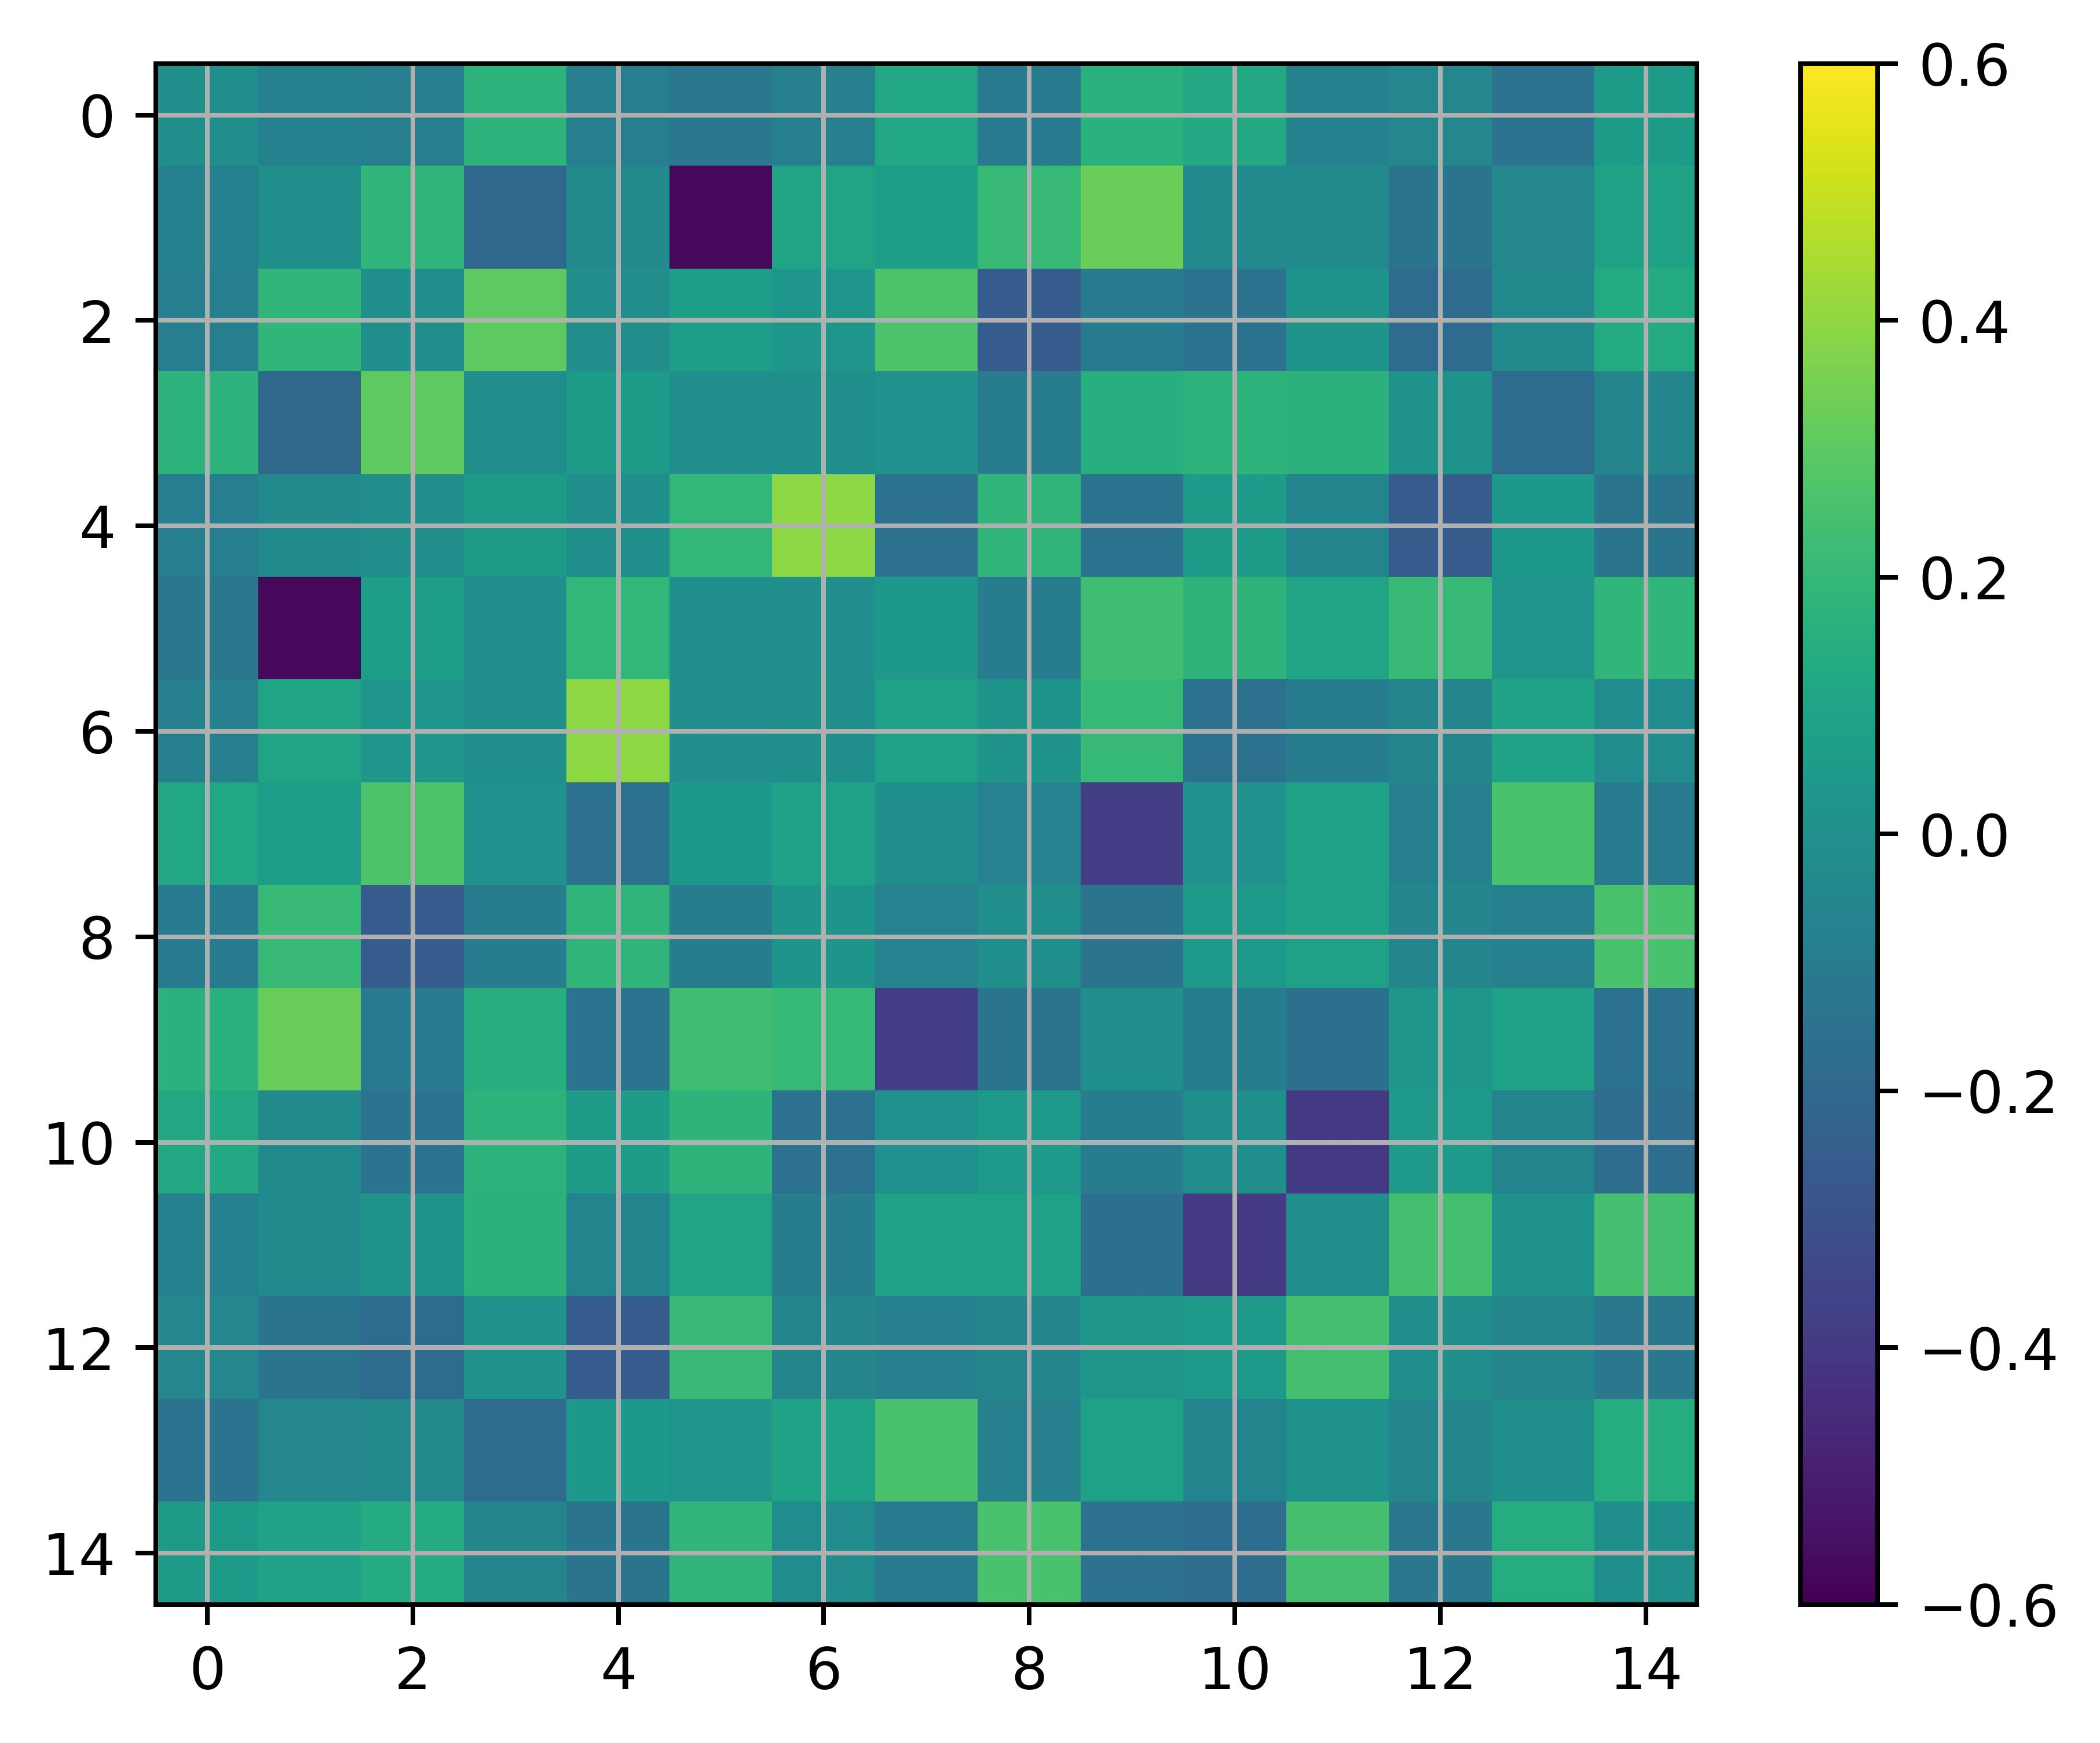
\includegraphics[width=1\textwidth]{../Analysis/DFC/size=480_step=180_rho=0.1/node=15_id=100206/0.jpg}
%                 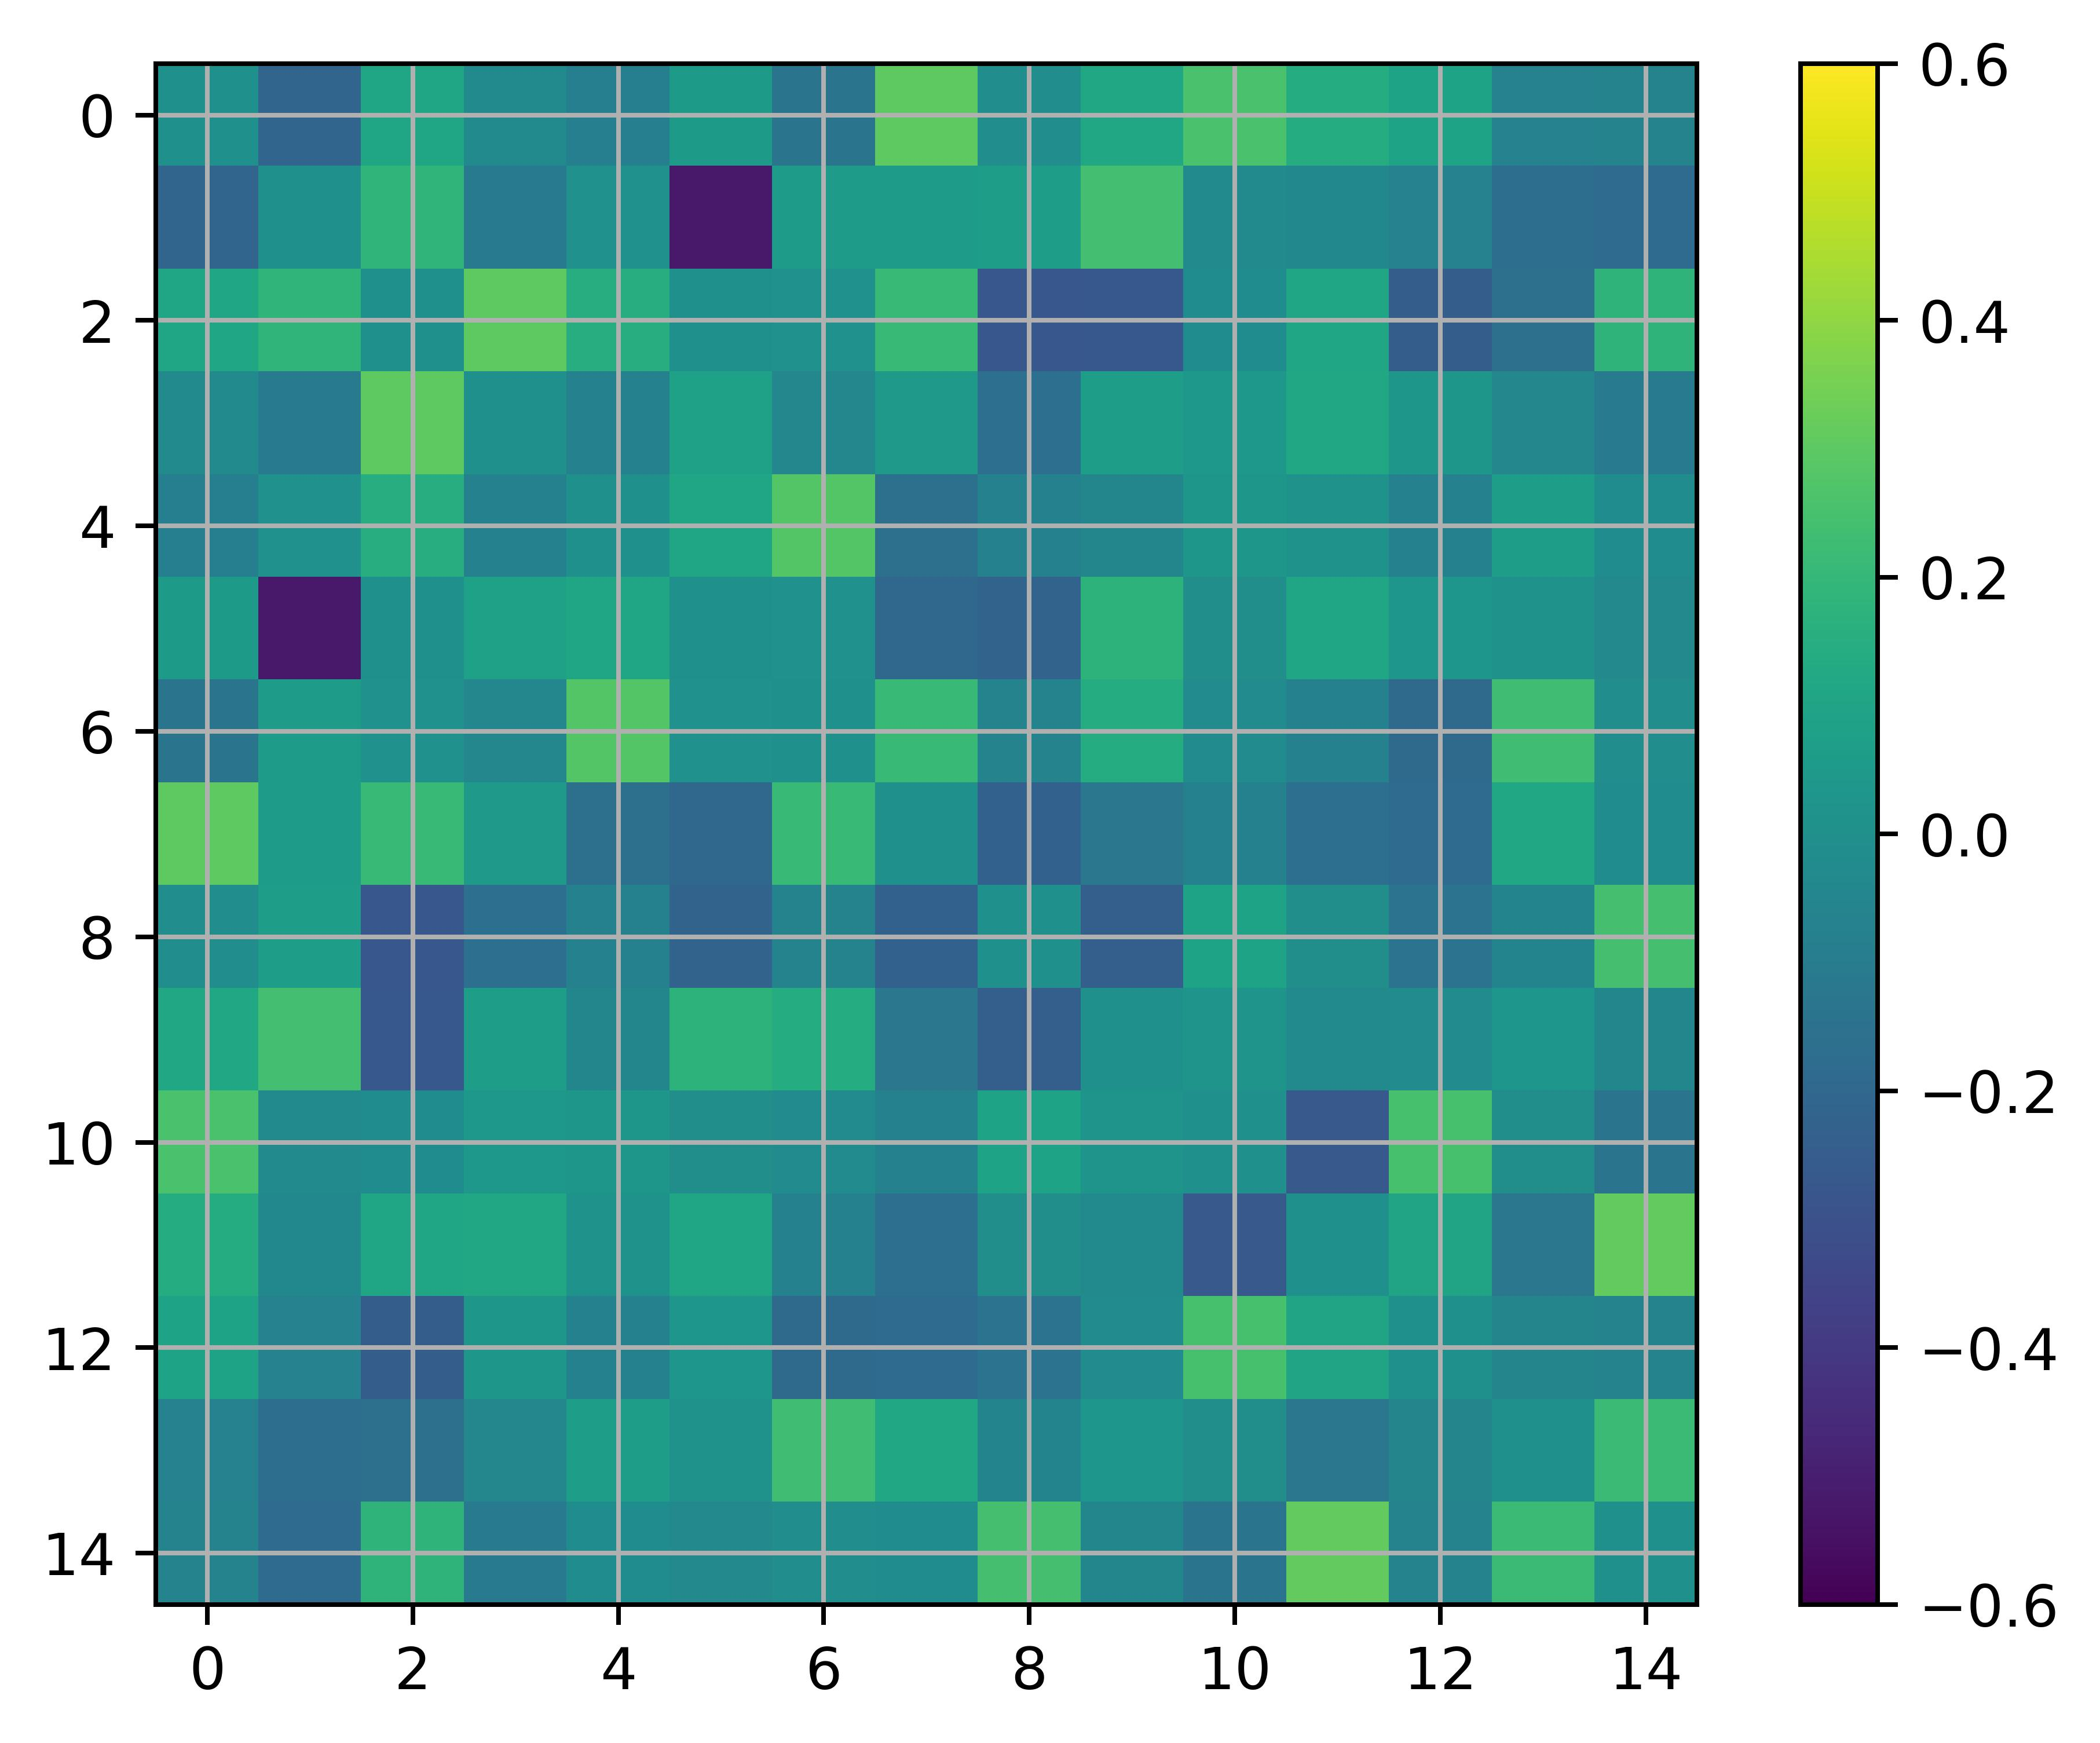
\includegraphics[width=1\textwidth]{../Analysis/DFC/size=480_step=180_rho=0.1/node=15_id=100206/10.jpg}
%                 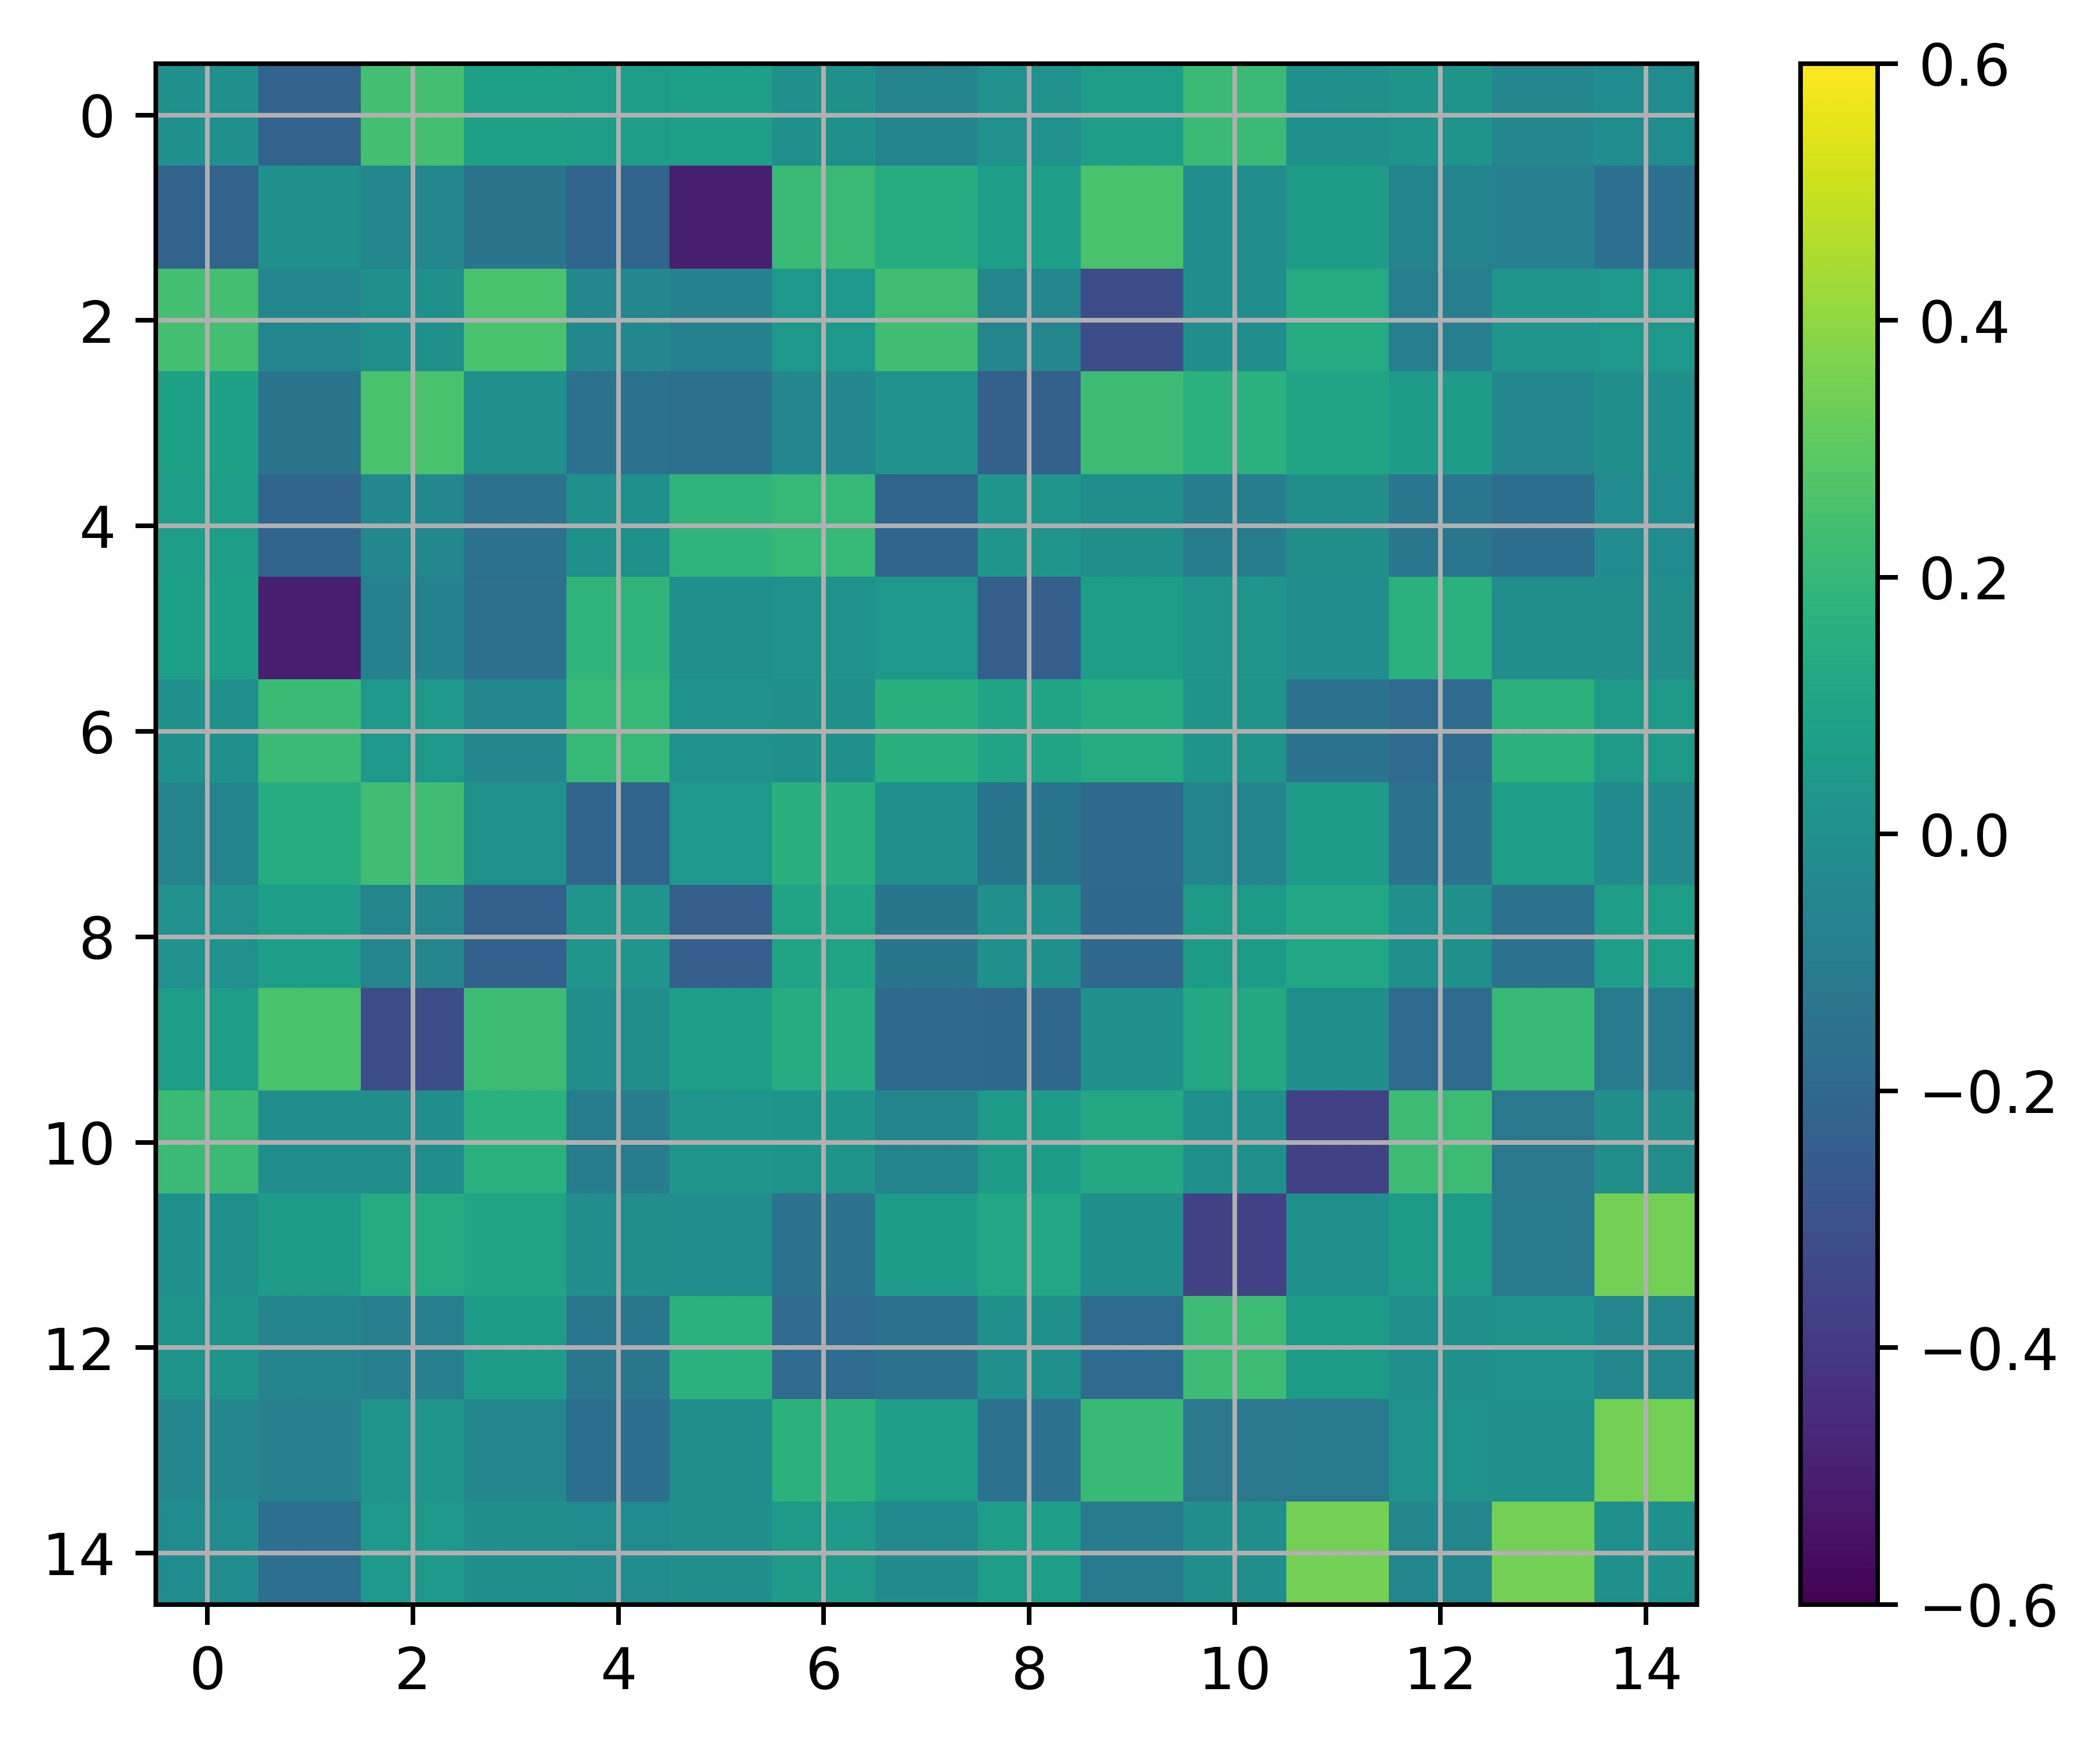
\includegraphics[width=1\textwidth]{../Analysis/DFC/size=480_step=180_rho=0.1/node=15_id=100206/20.jpg}
%             \end{minipage}
%         }
%         \subfloat[$N_{node} = 25$]{
%             \begin{minipage}[b]{0.2\textwidth}
%                 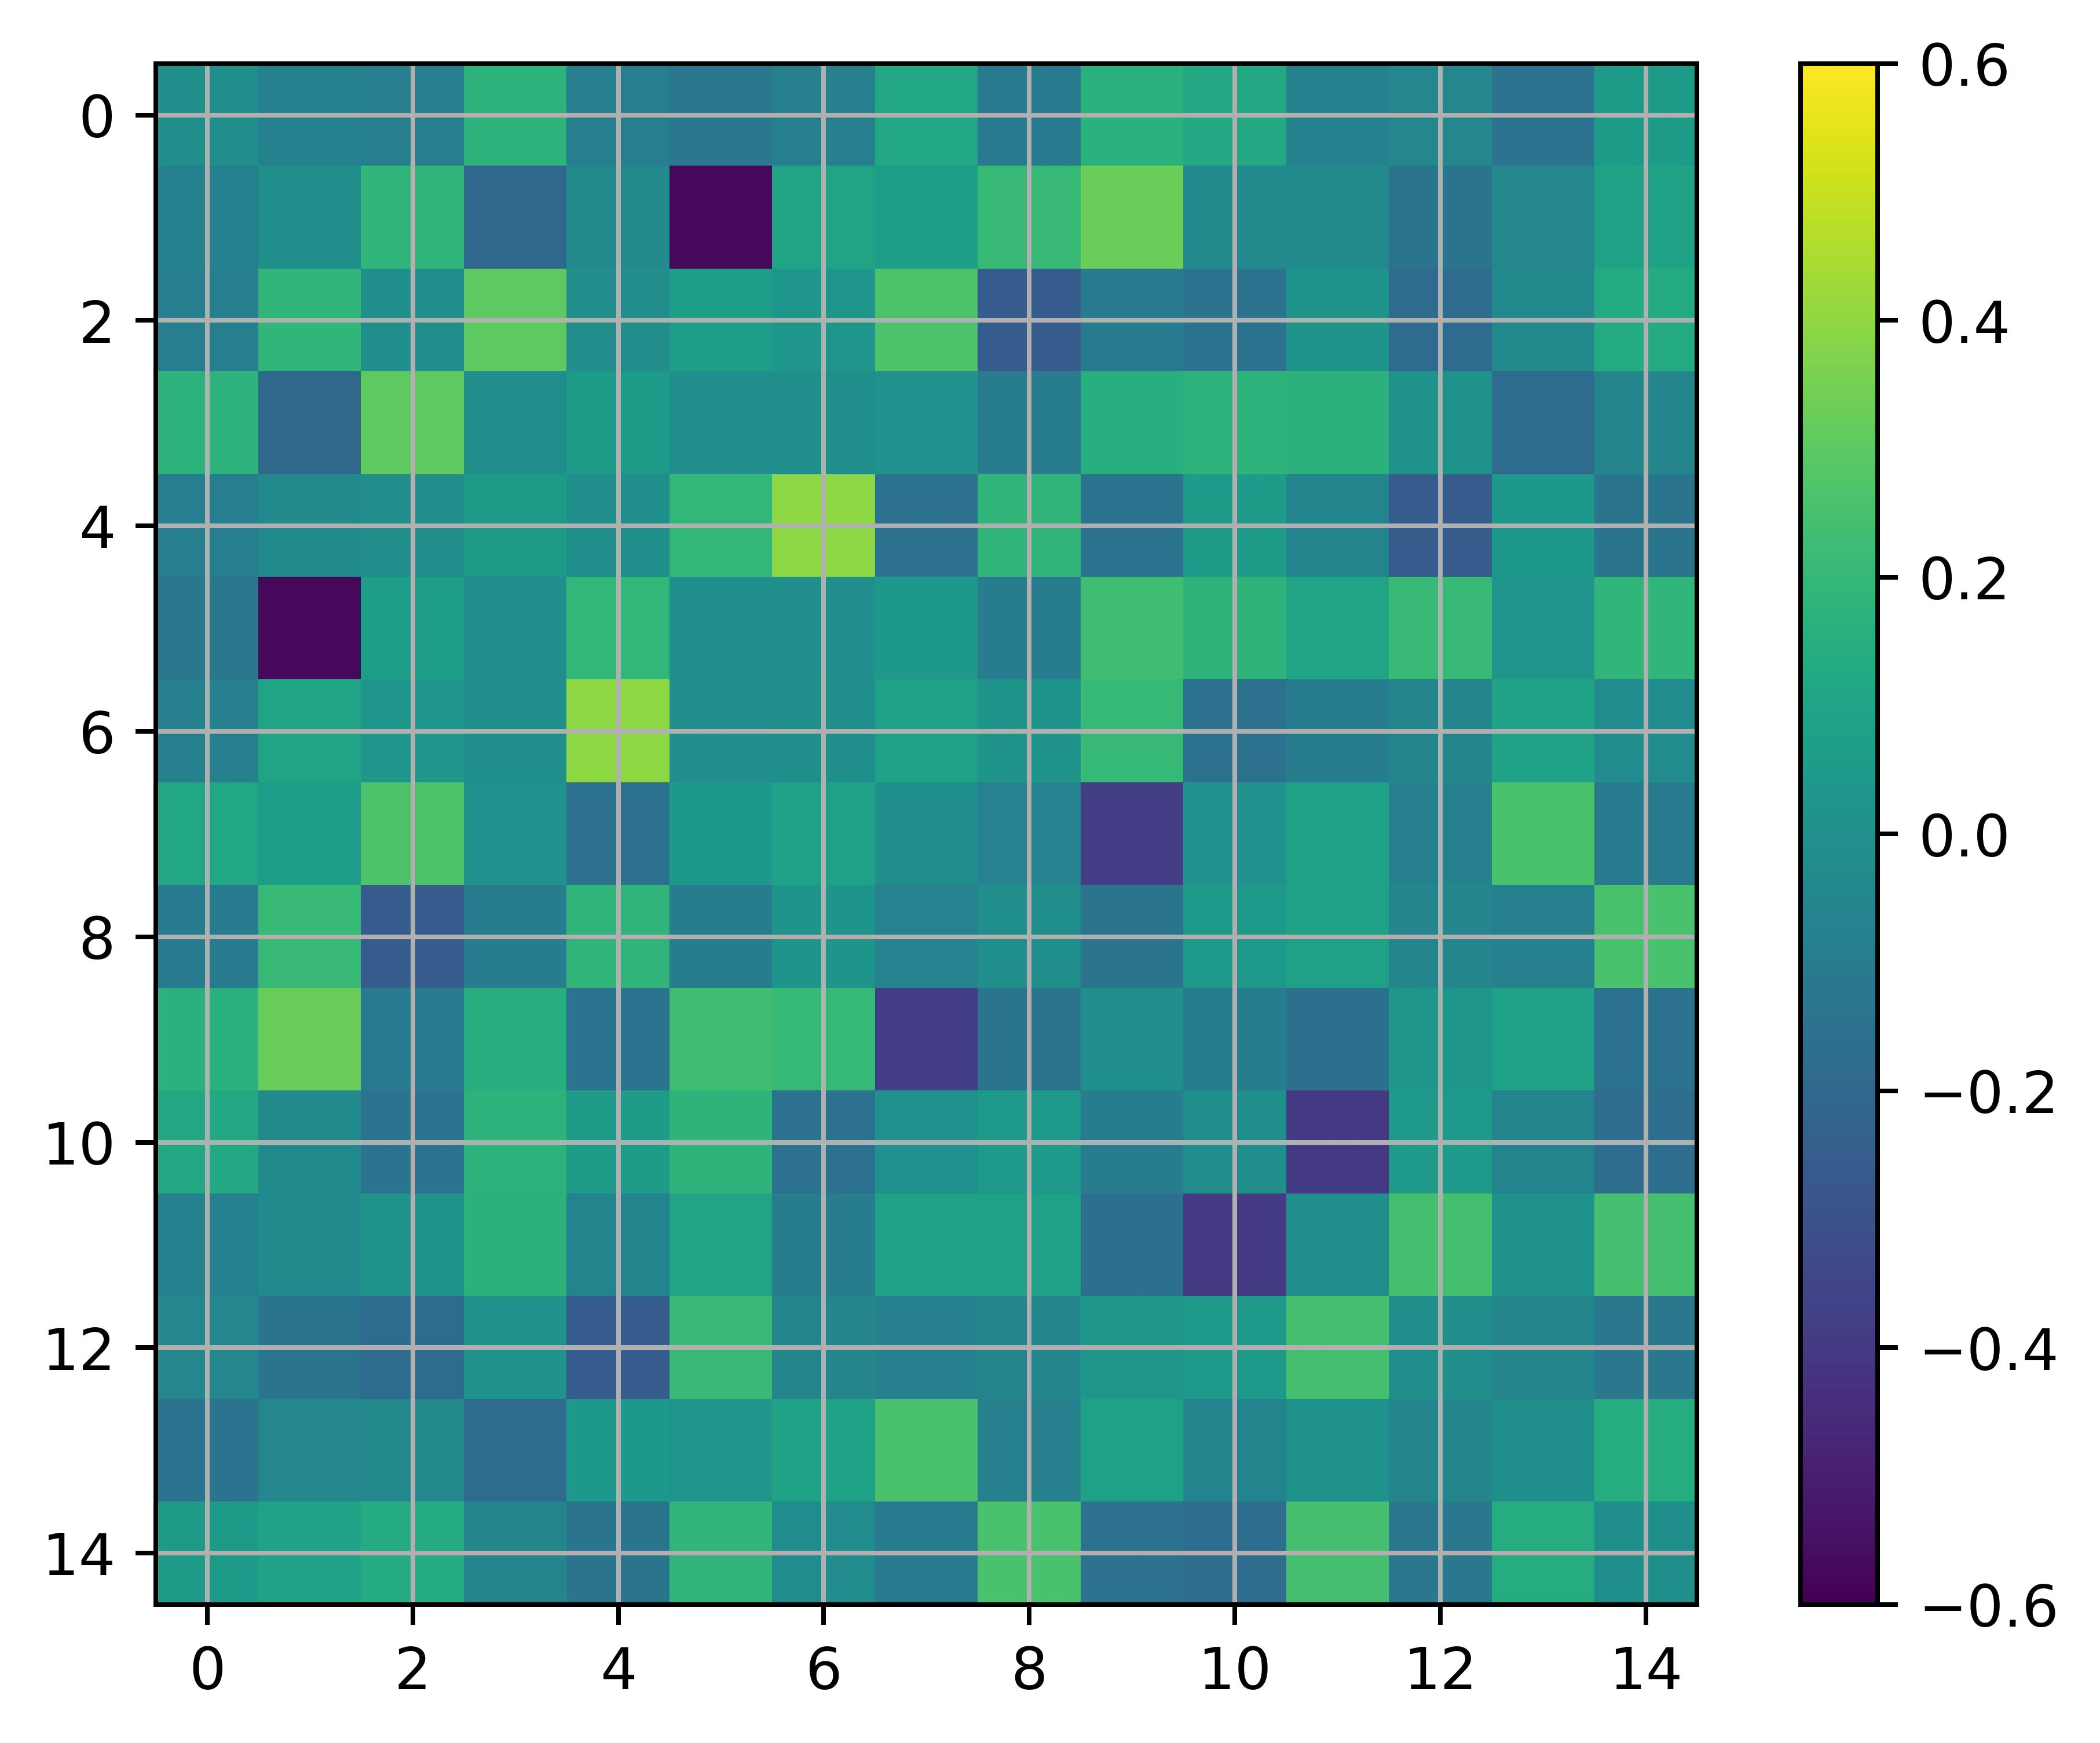
\includegraphics[width=1\textwidth]{../Analysis/DFC/size=480_step=180_rho=0.1/node=15_id=100206/0.jpg}
%                 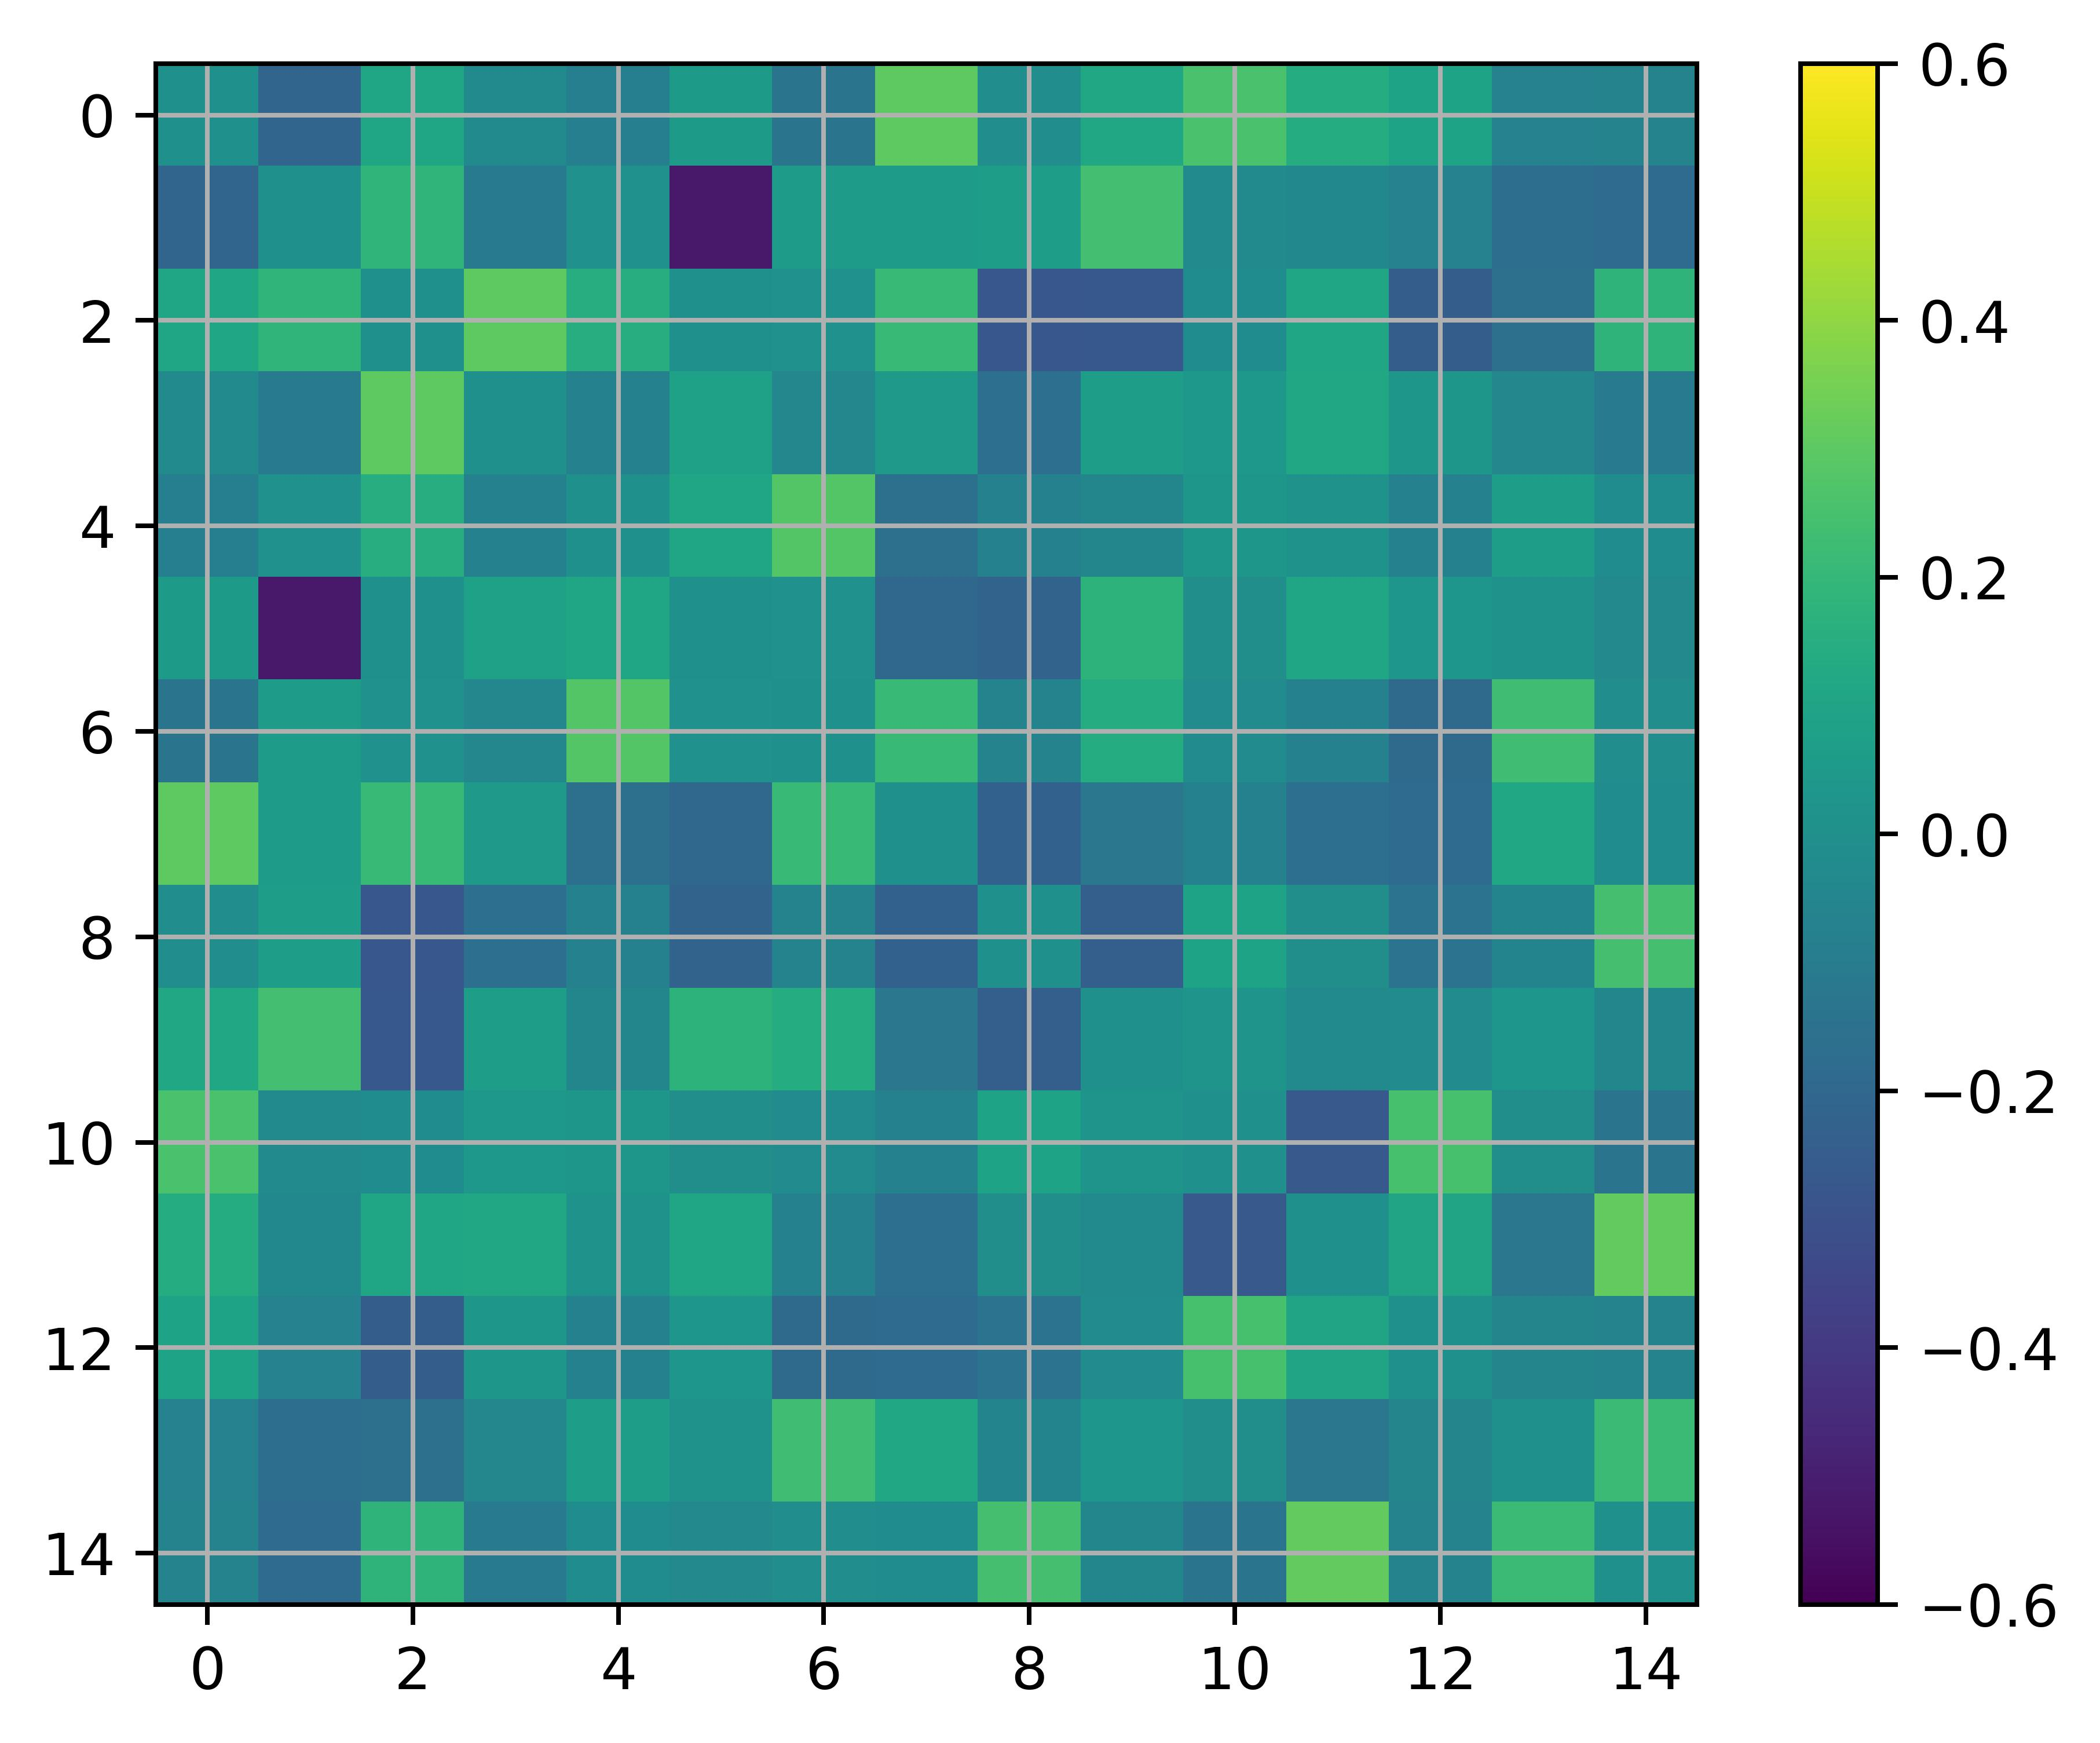
\includegraphics[width=1\textwidth]{../Analysis/DFC/size=480_step=180_rho=0.1/node=15_id=100206/10.jpg}
%                 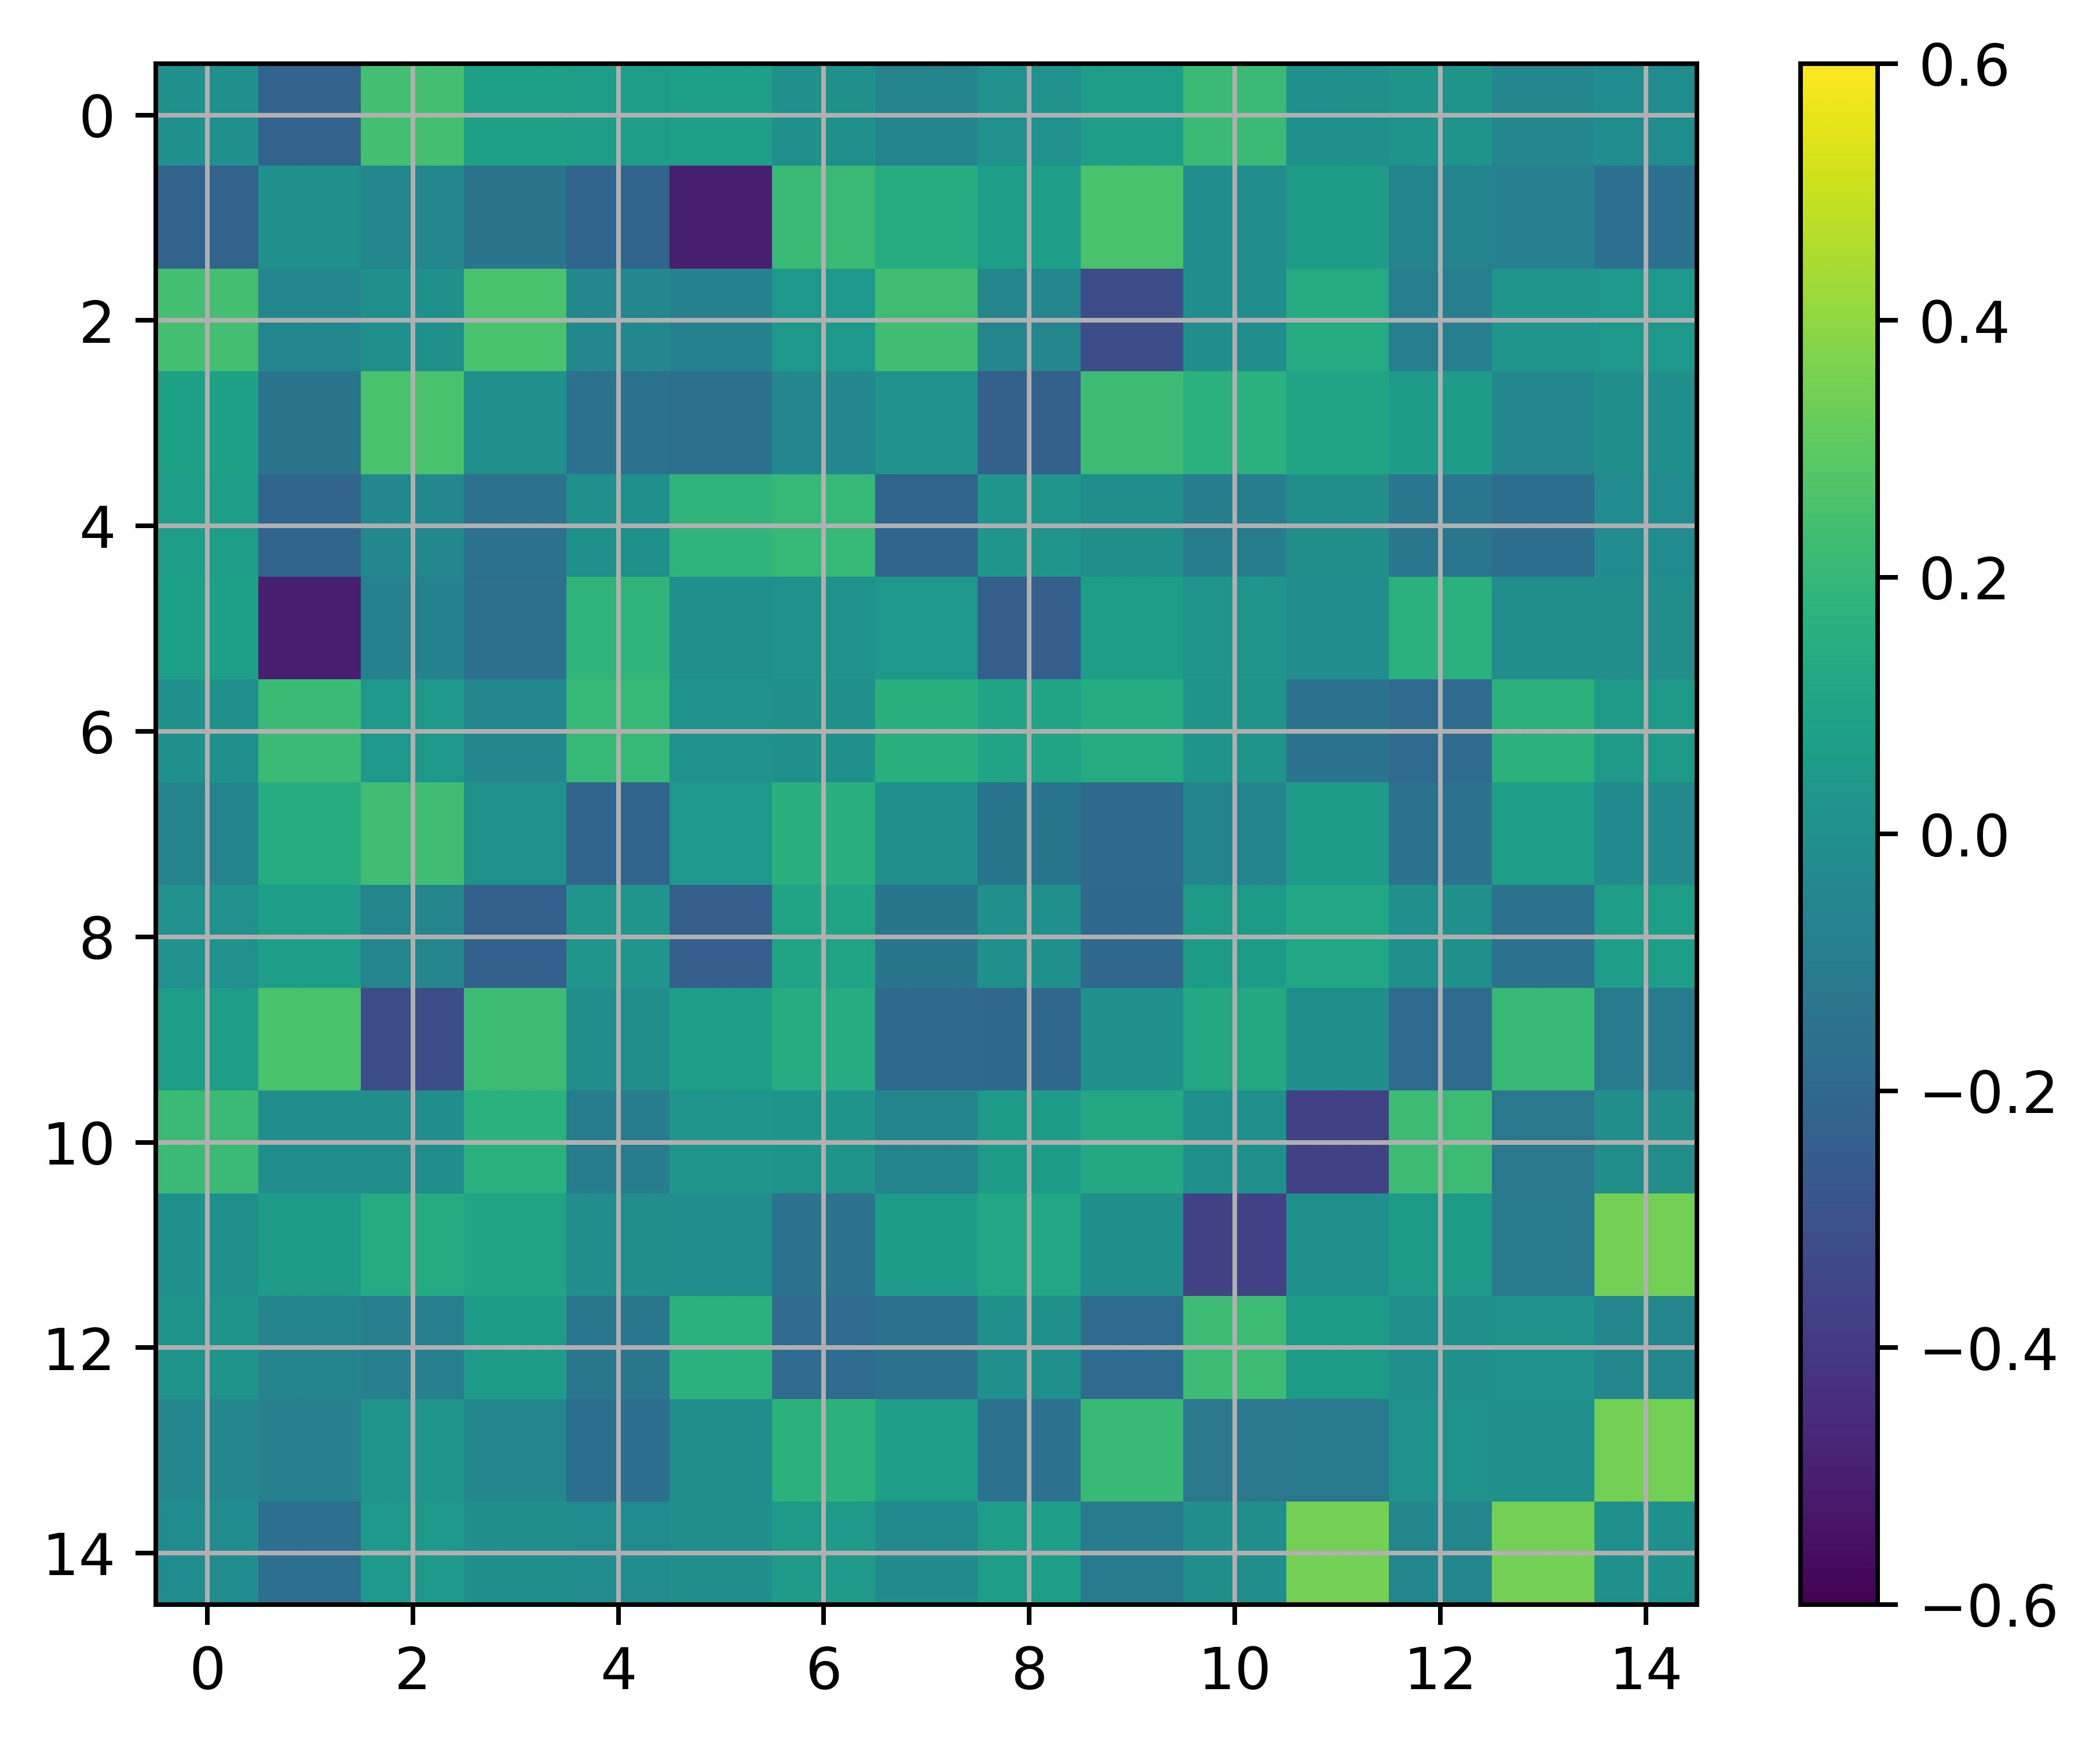
\includegraphics[width=1\textwidth]{../Analysis/DFC/size=480_step=180_rho=0.1/node=15_id=100206/20.jpg}
%             \end{minipage}
%         }
%         \subfloat[$N_{node} = 50$]{
%             \begin{minipage}[b]{0.2\textwidth}
%                 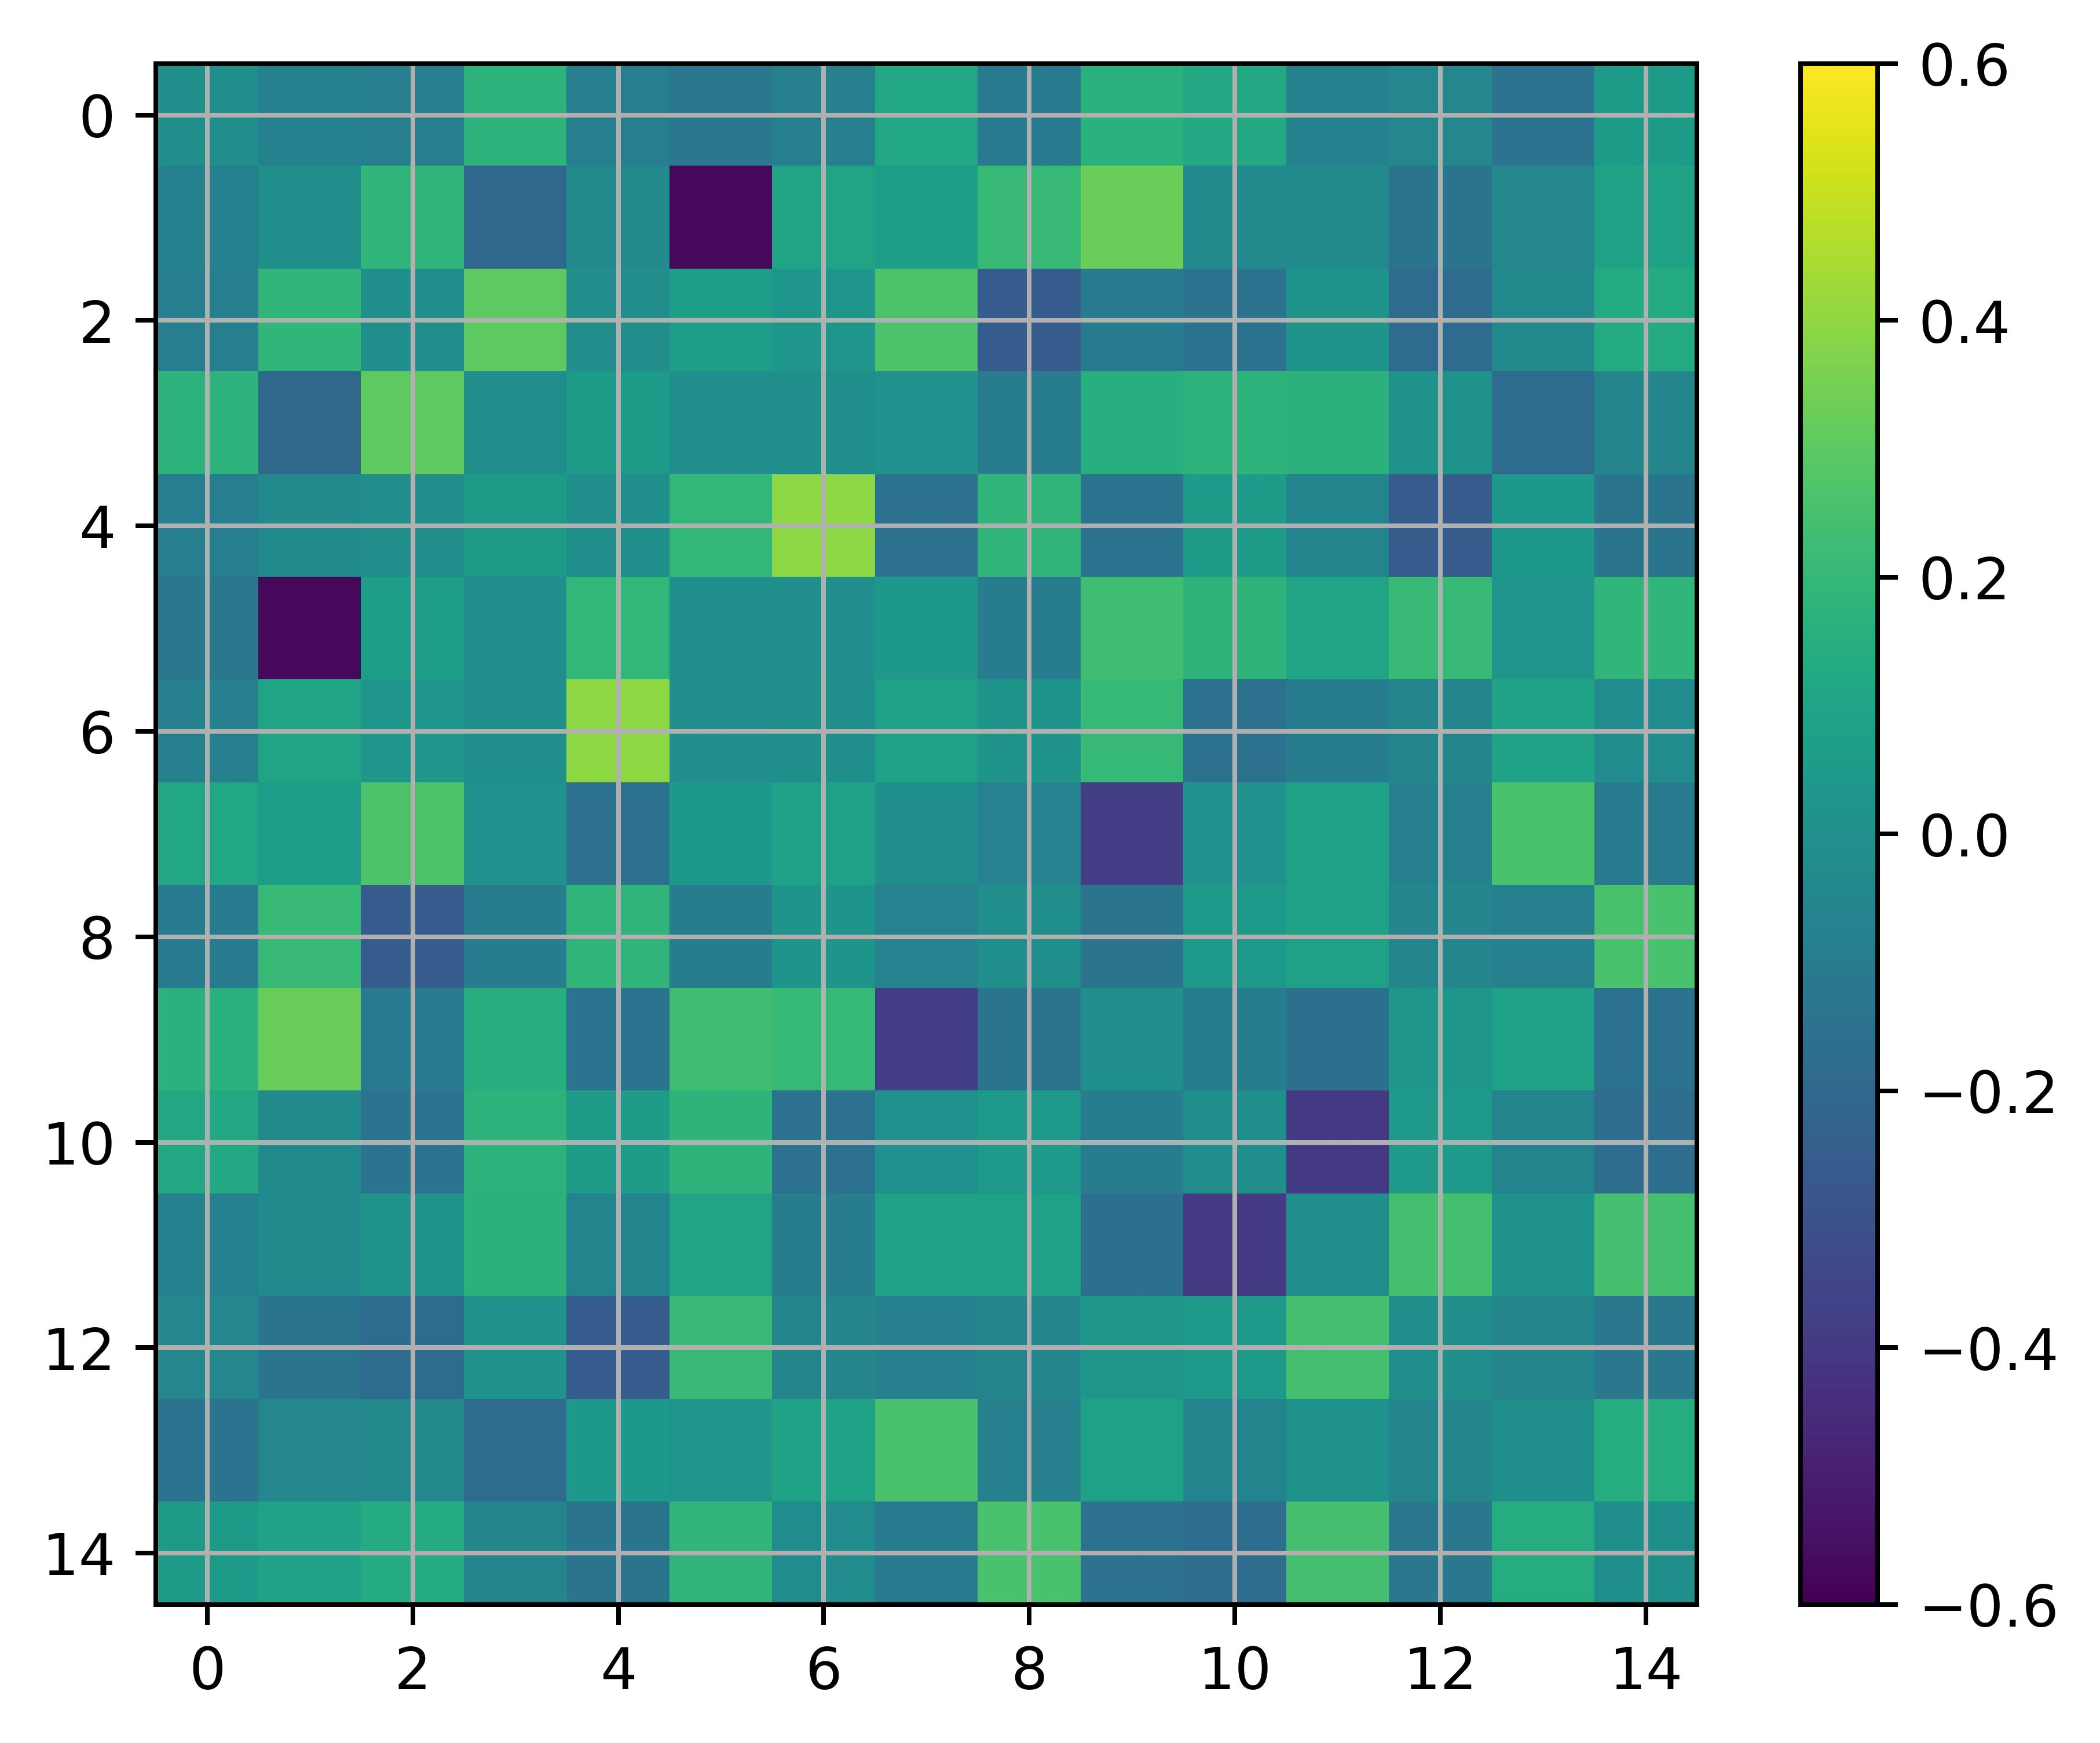
\includegraphics[width=1\textwidth]{../Analysis/DFC/size=480_step=180_rho=0.1/node=15_id=100206/0.jpg}
%                 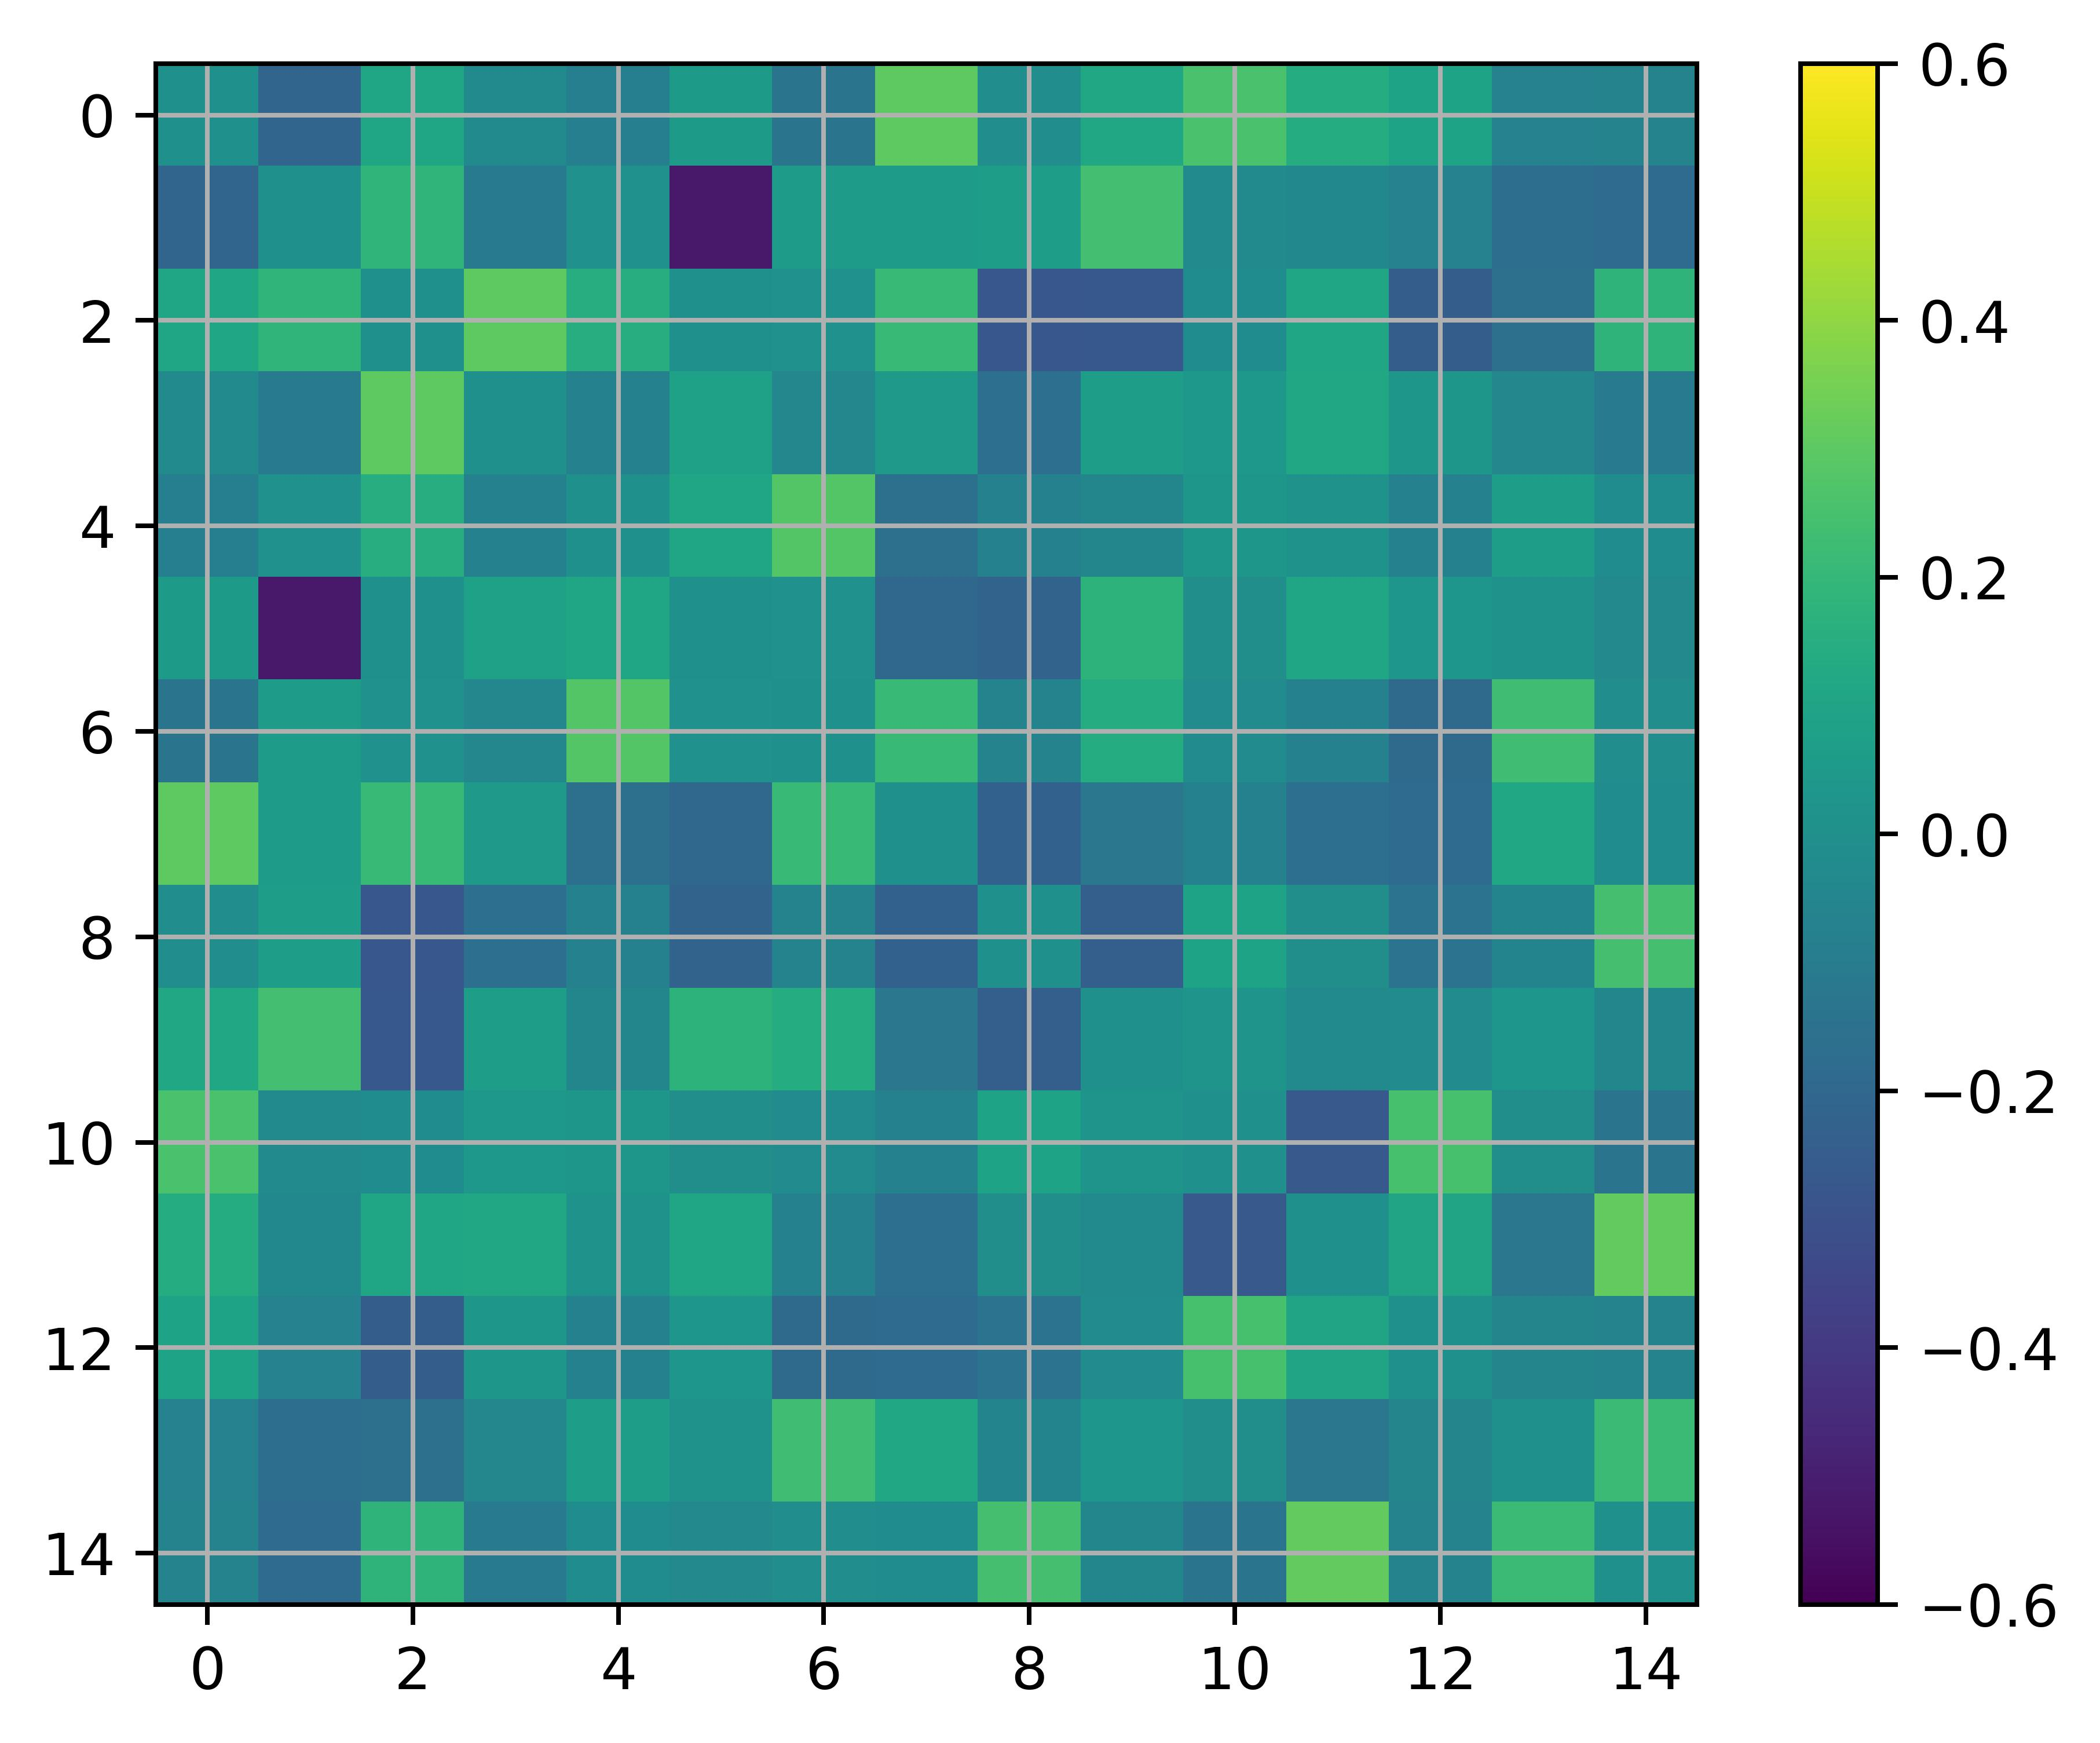
\includegraphics[width=1\textwidth]{../Analysis/DFC/size=480_step=180_rho=0.1/node=15_id=100206/10.jpg}
%                 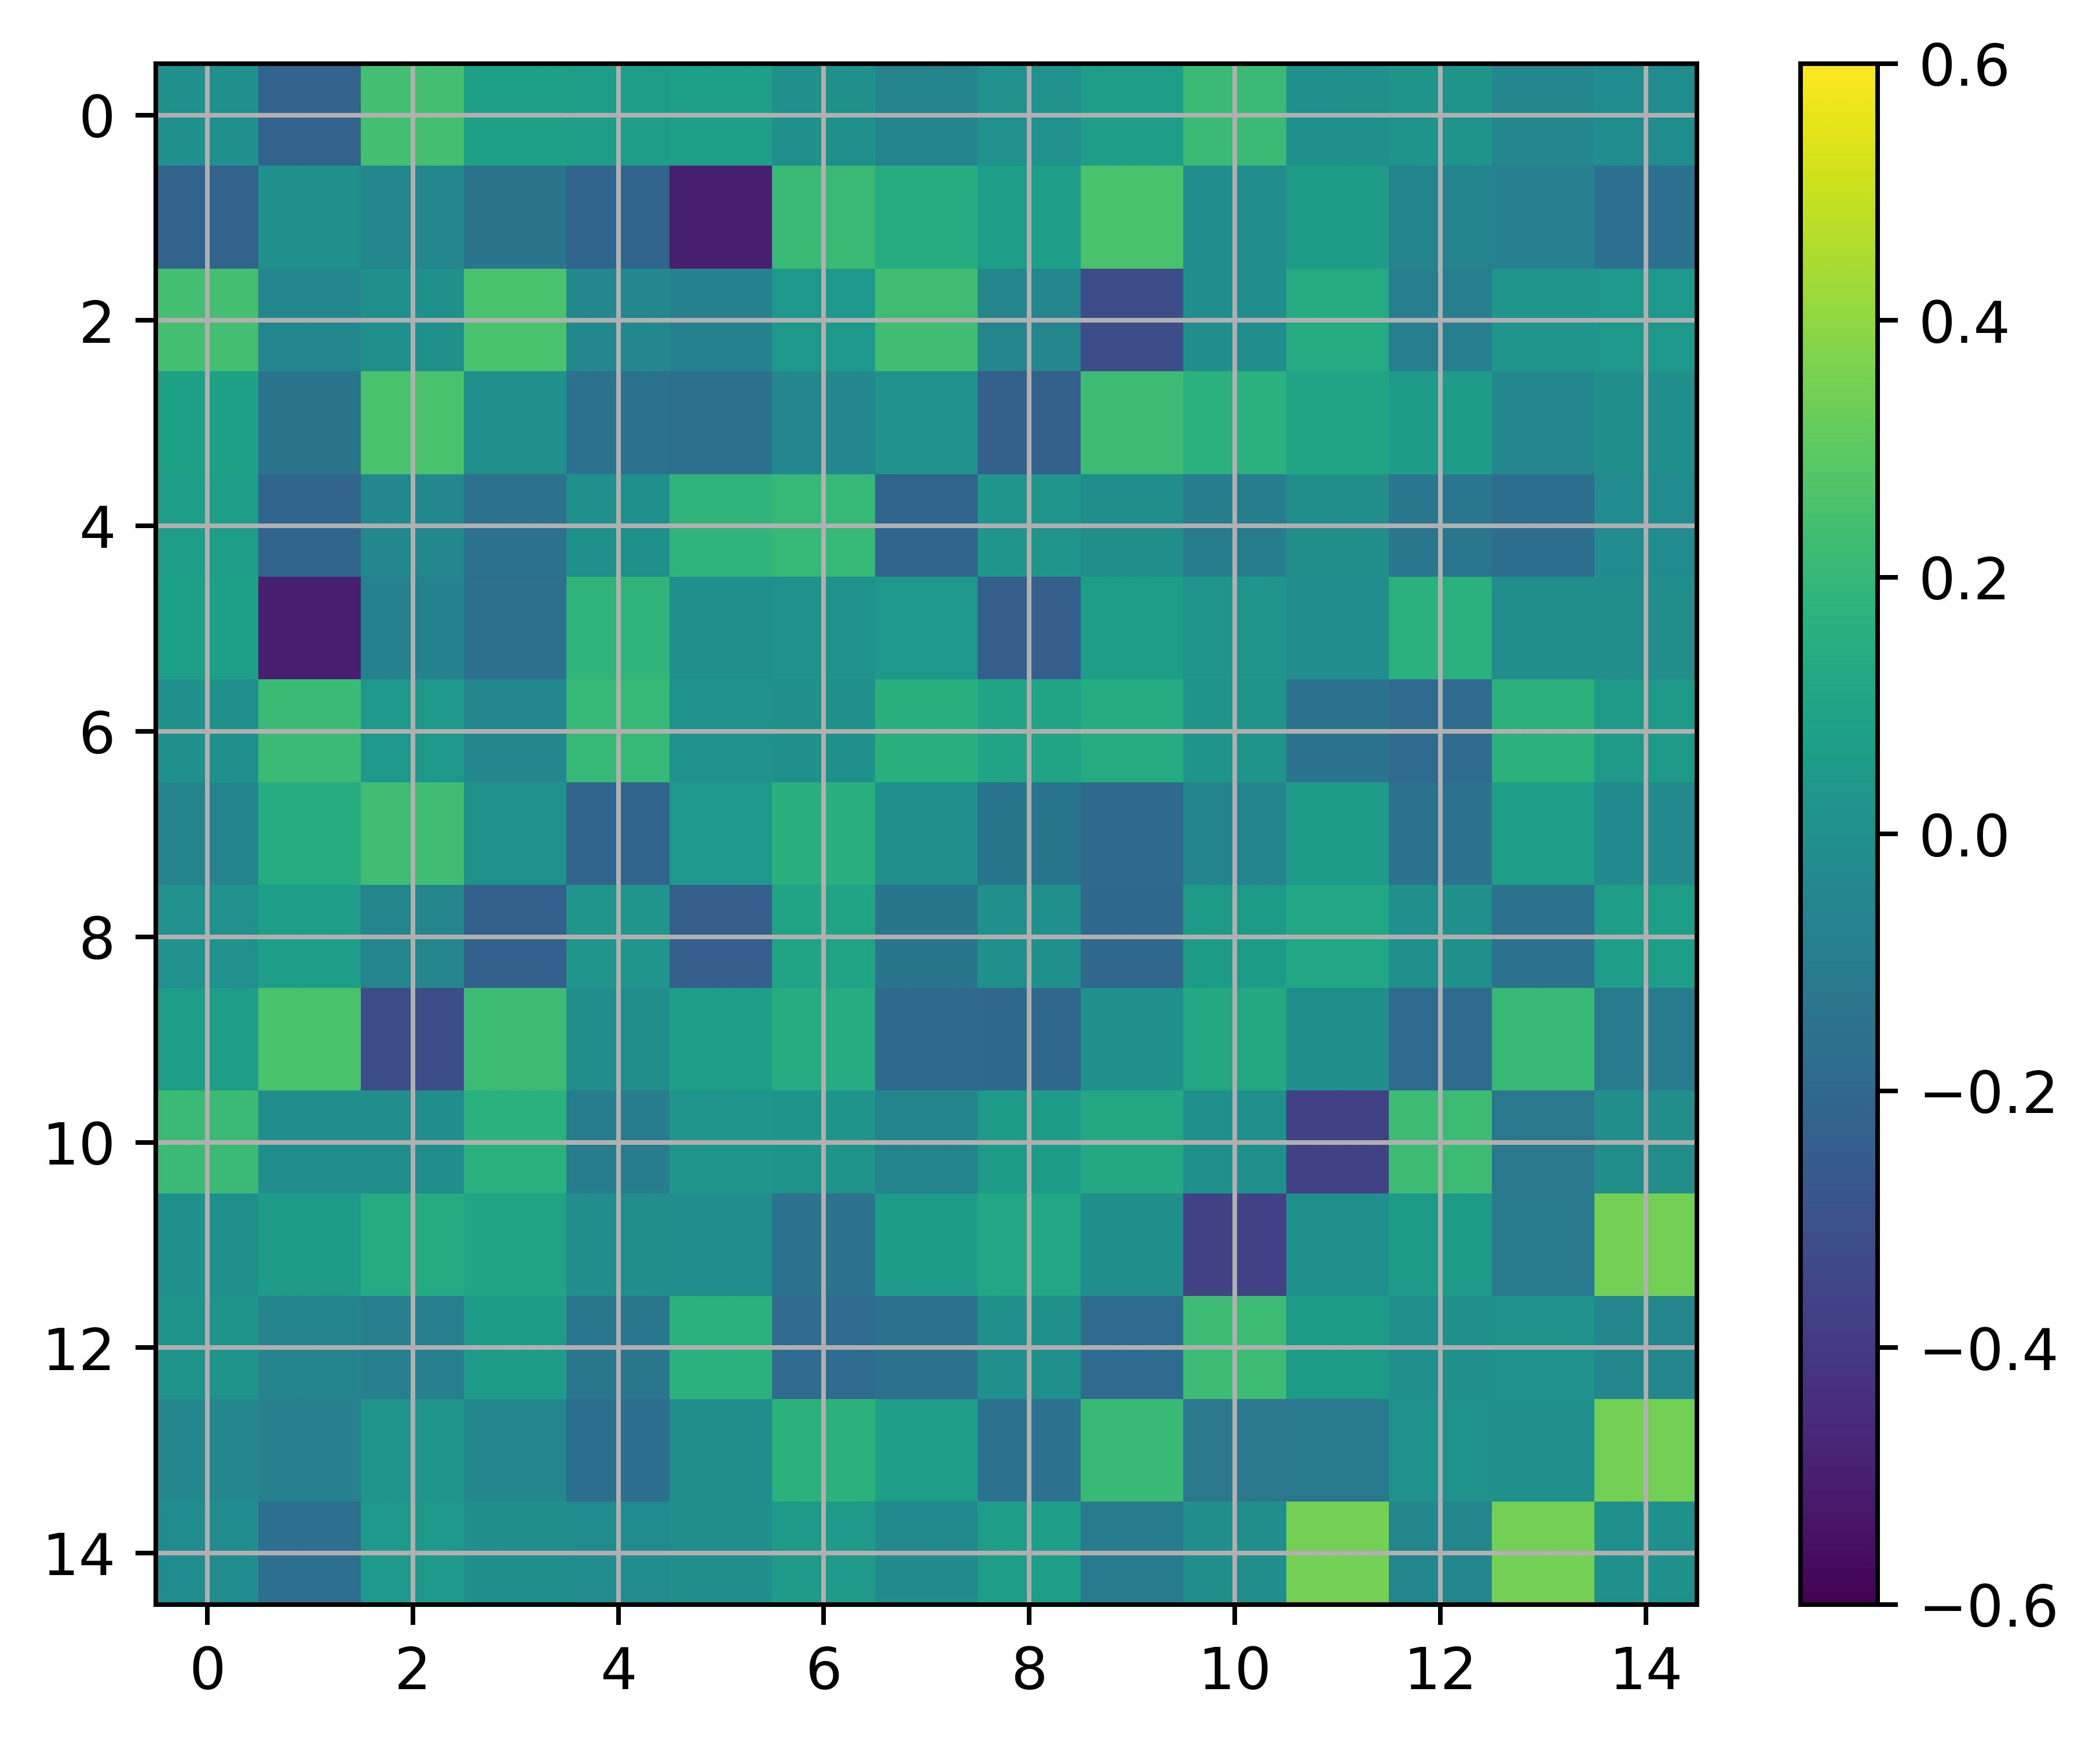
\includegraphics[width=1\textwidth]{../Analysis/DFC/size=480_step=180_rho=0.1/node=15_id=100206/20.jpg}
%             \end{minipage}
%         }
%         % \caption{LDA for static connectivity with $N_{node} = 15$.}
%         % \label{LDA-example-1}
%     \end{figure}

% \end{frame}

\begin{frame}{Preprocessing - Examples}

    \begin{figure}[H]
        \centering
        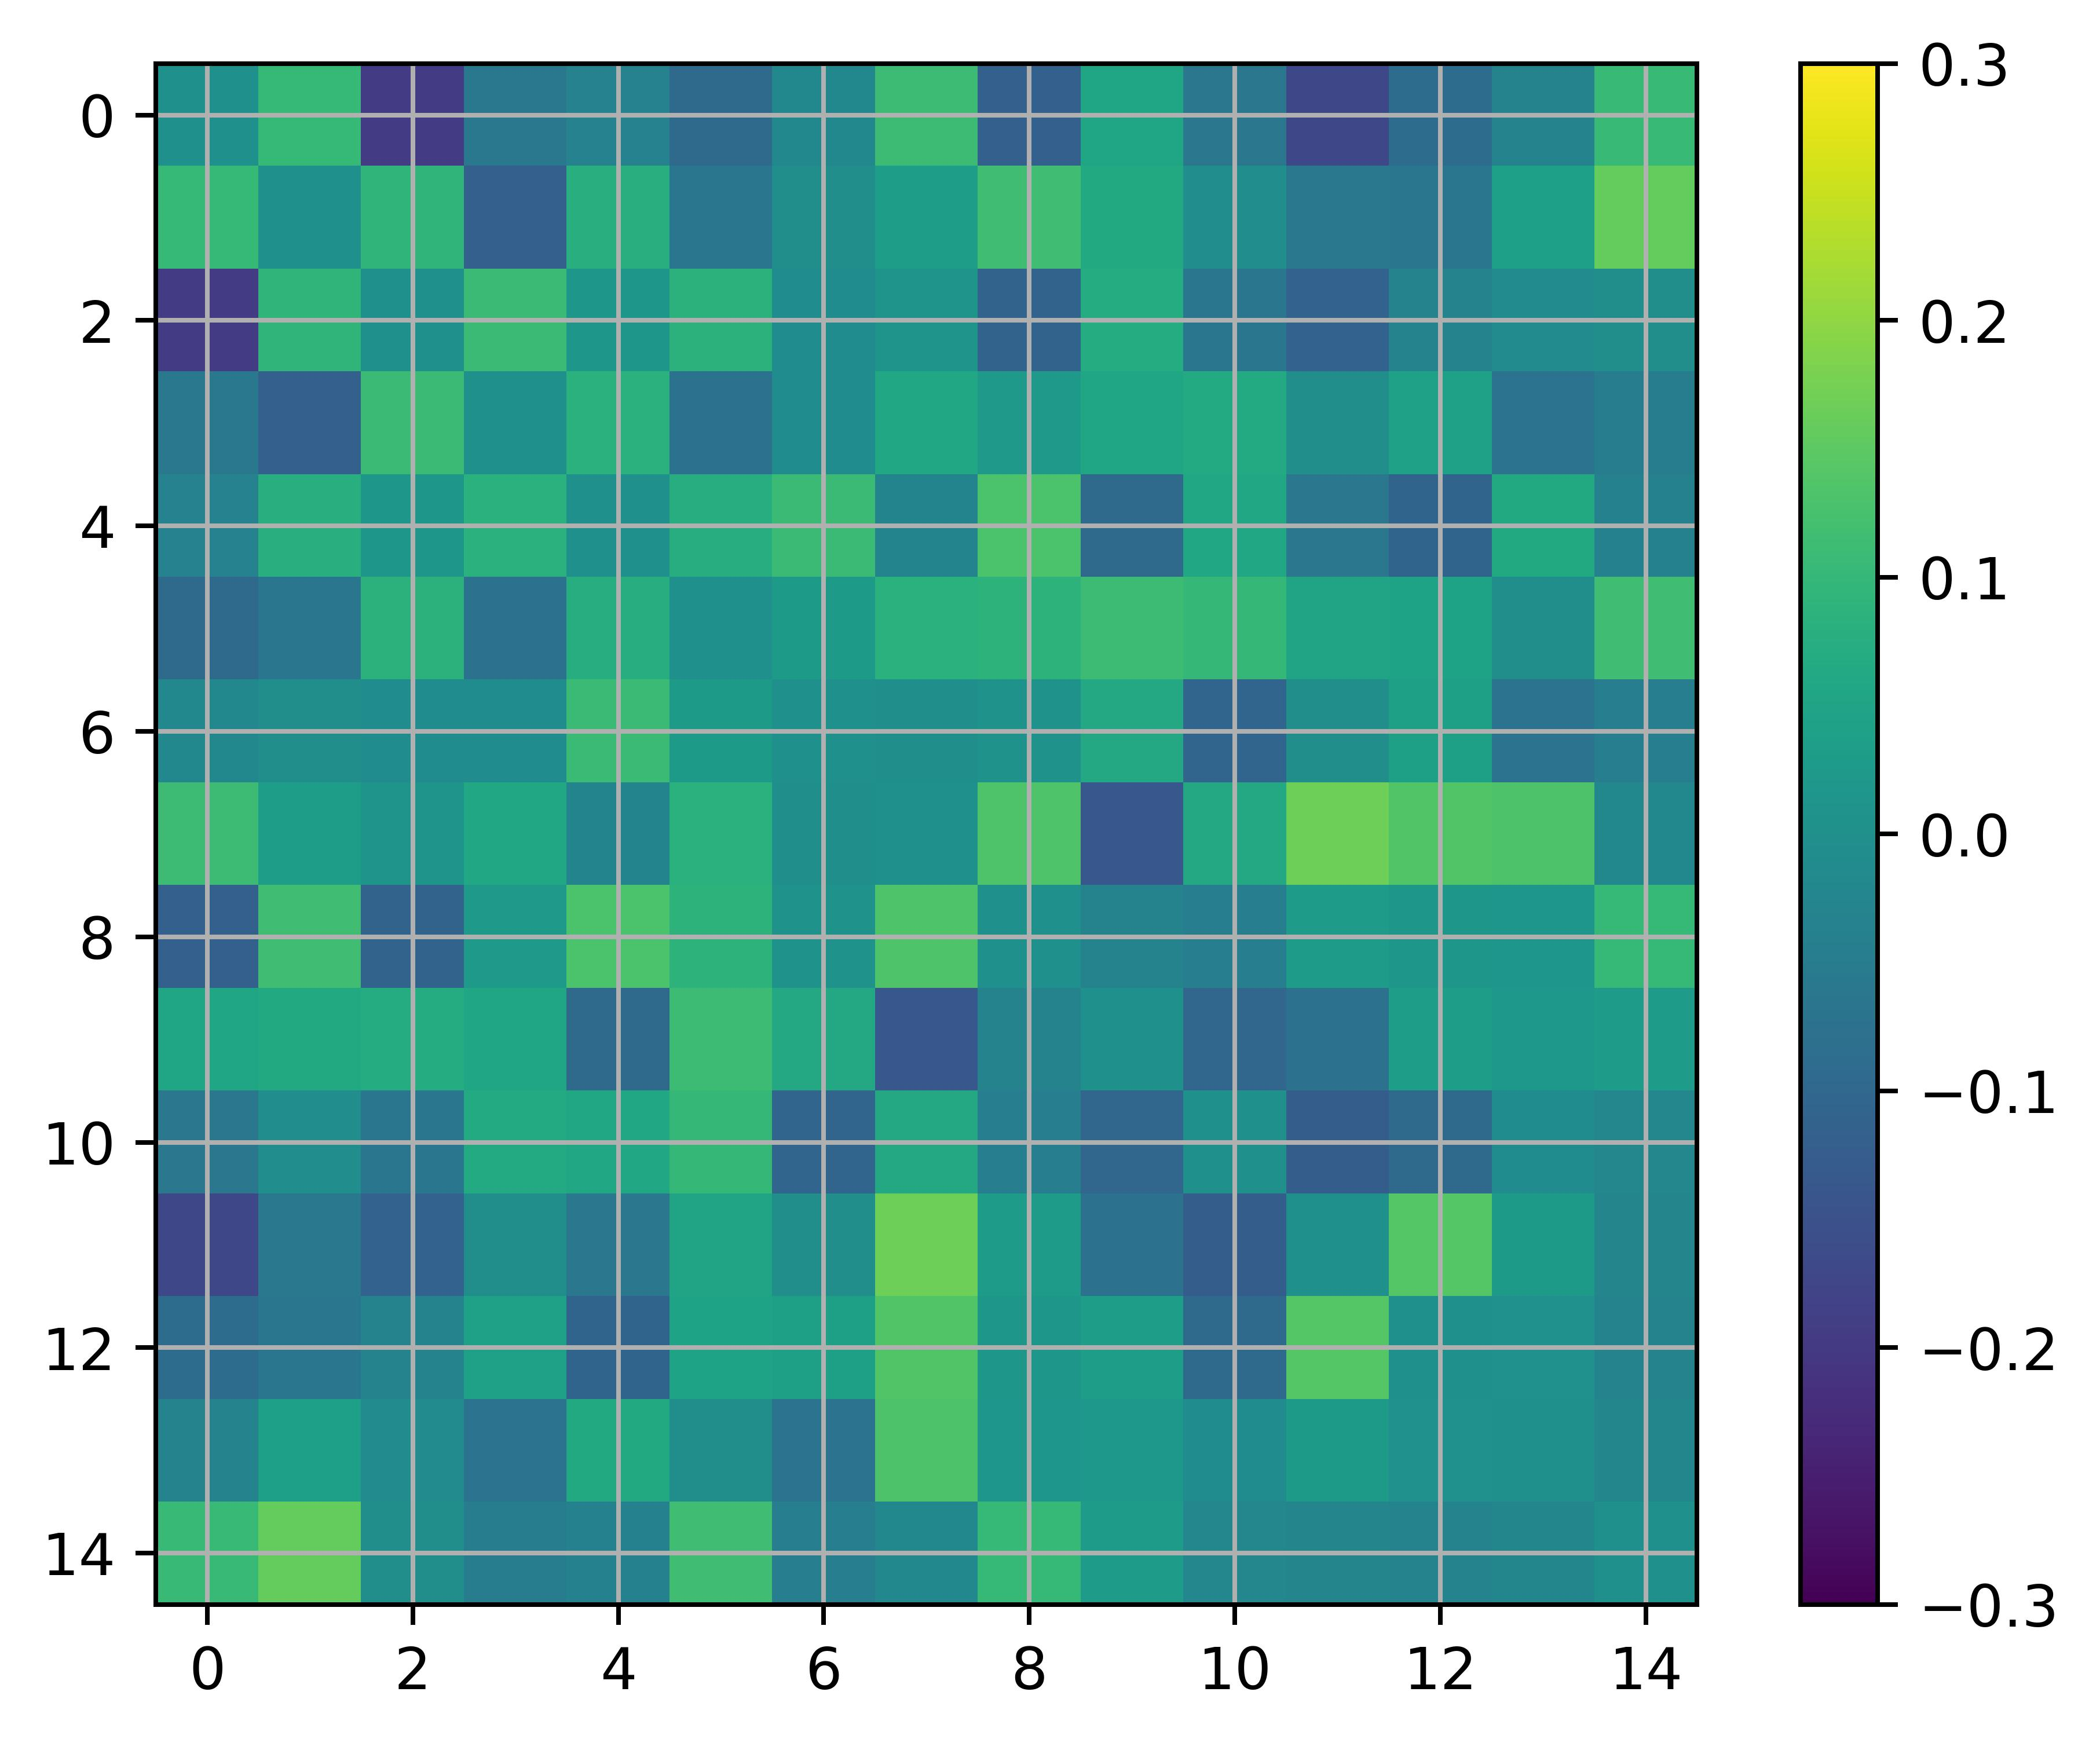
\includegraphics[width=0.2\textwidth]{../Analysis/DFC/size=480_step=180_rho=0.1/node=15_id=100206/c_0.jpg}
        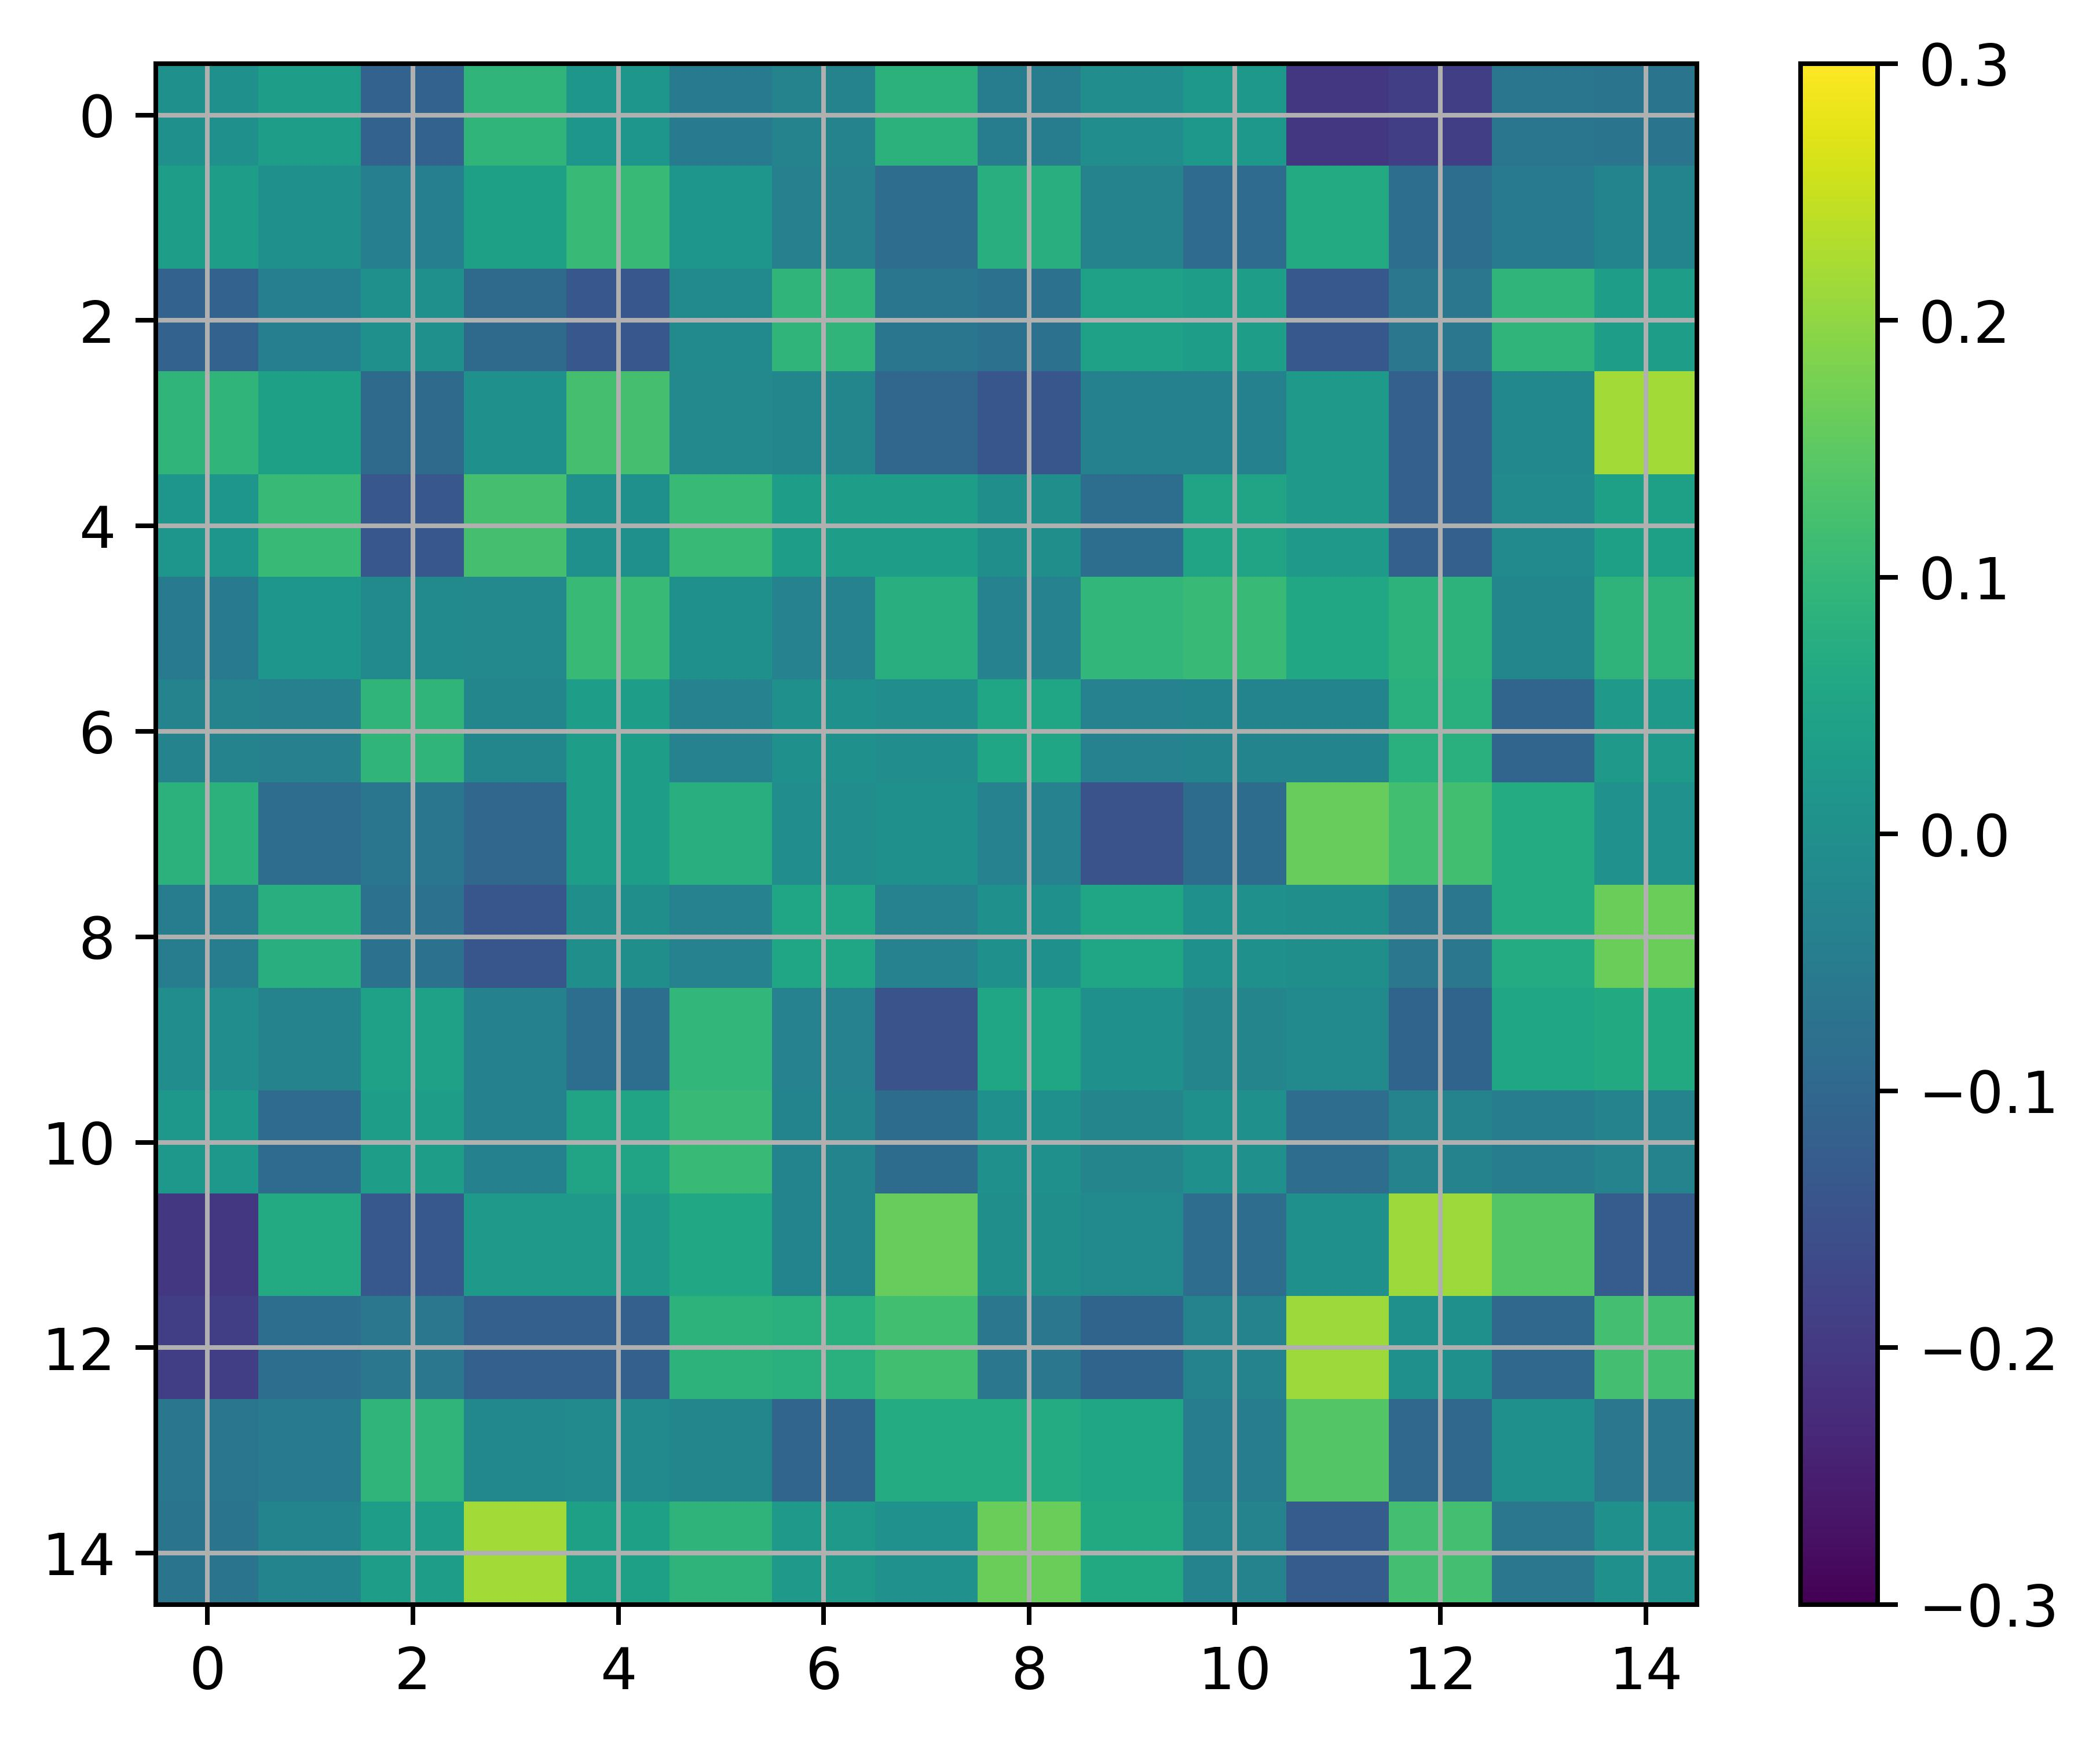
\includegraphics[width=0.2\textwidth]{../Analysis/DFC/size=480_step=180_rho=0.1/node=15_id=100206/c_2.jpg}
        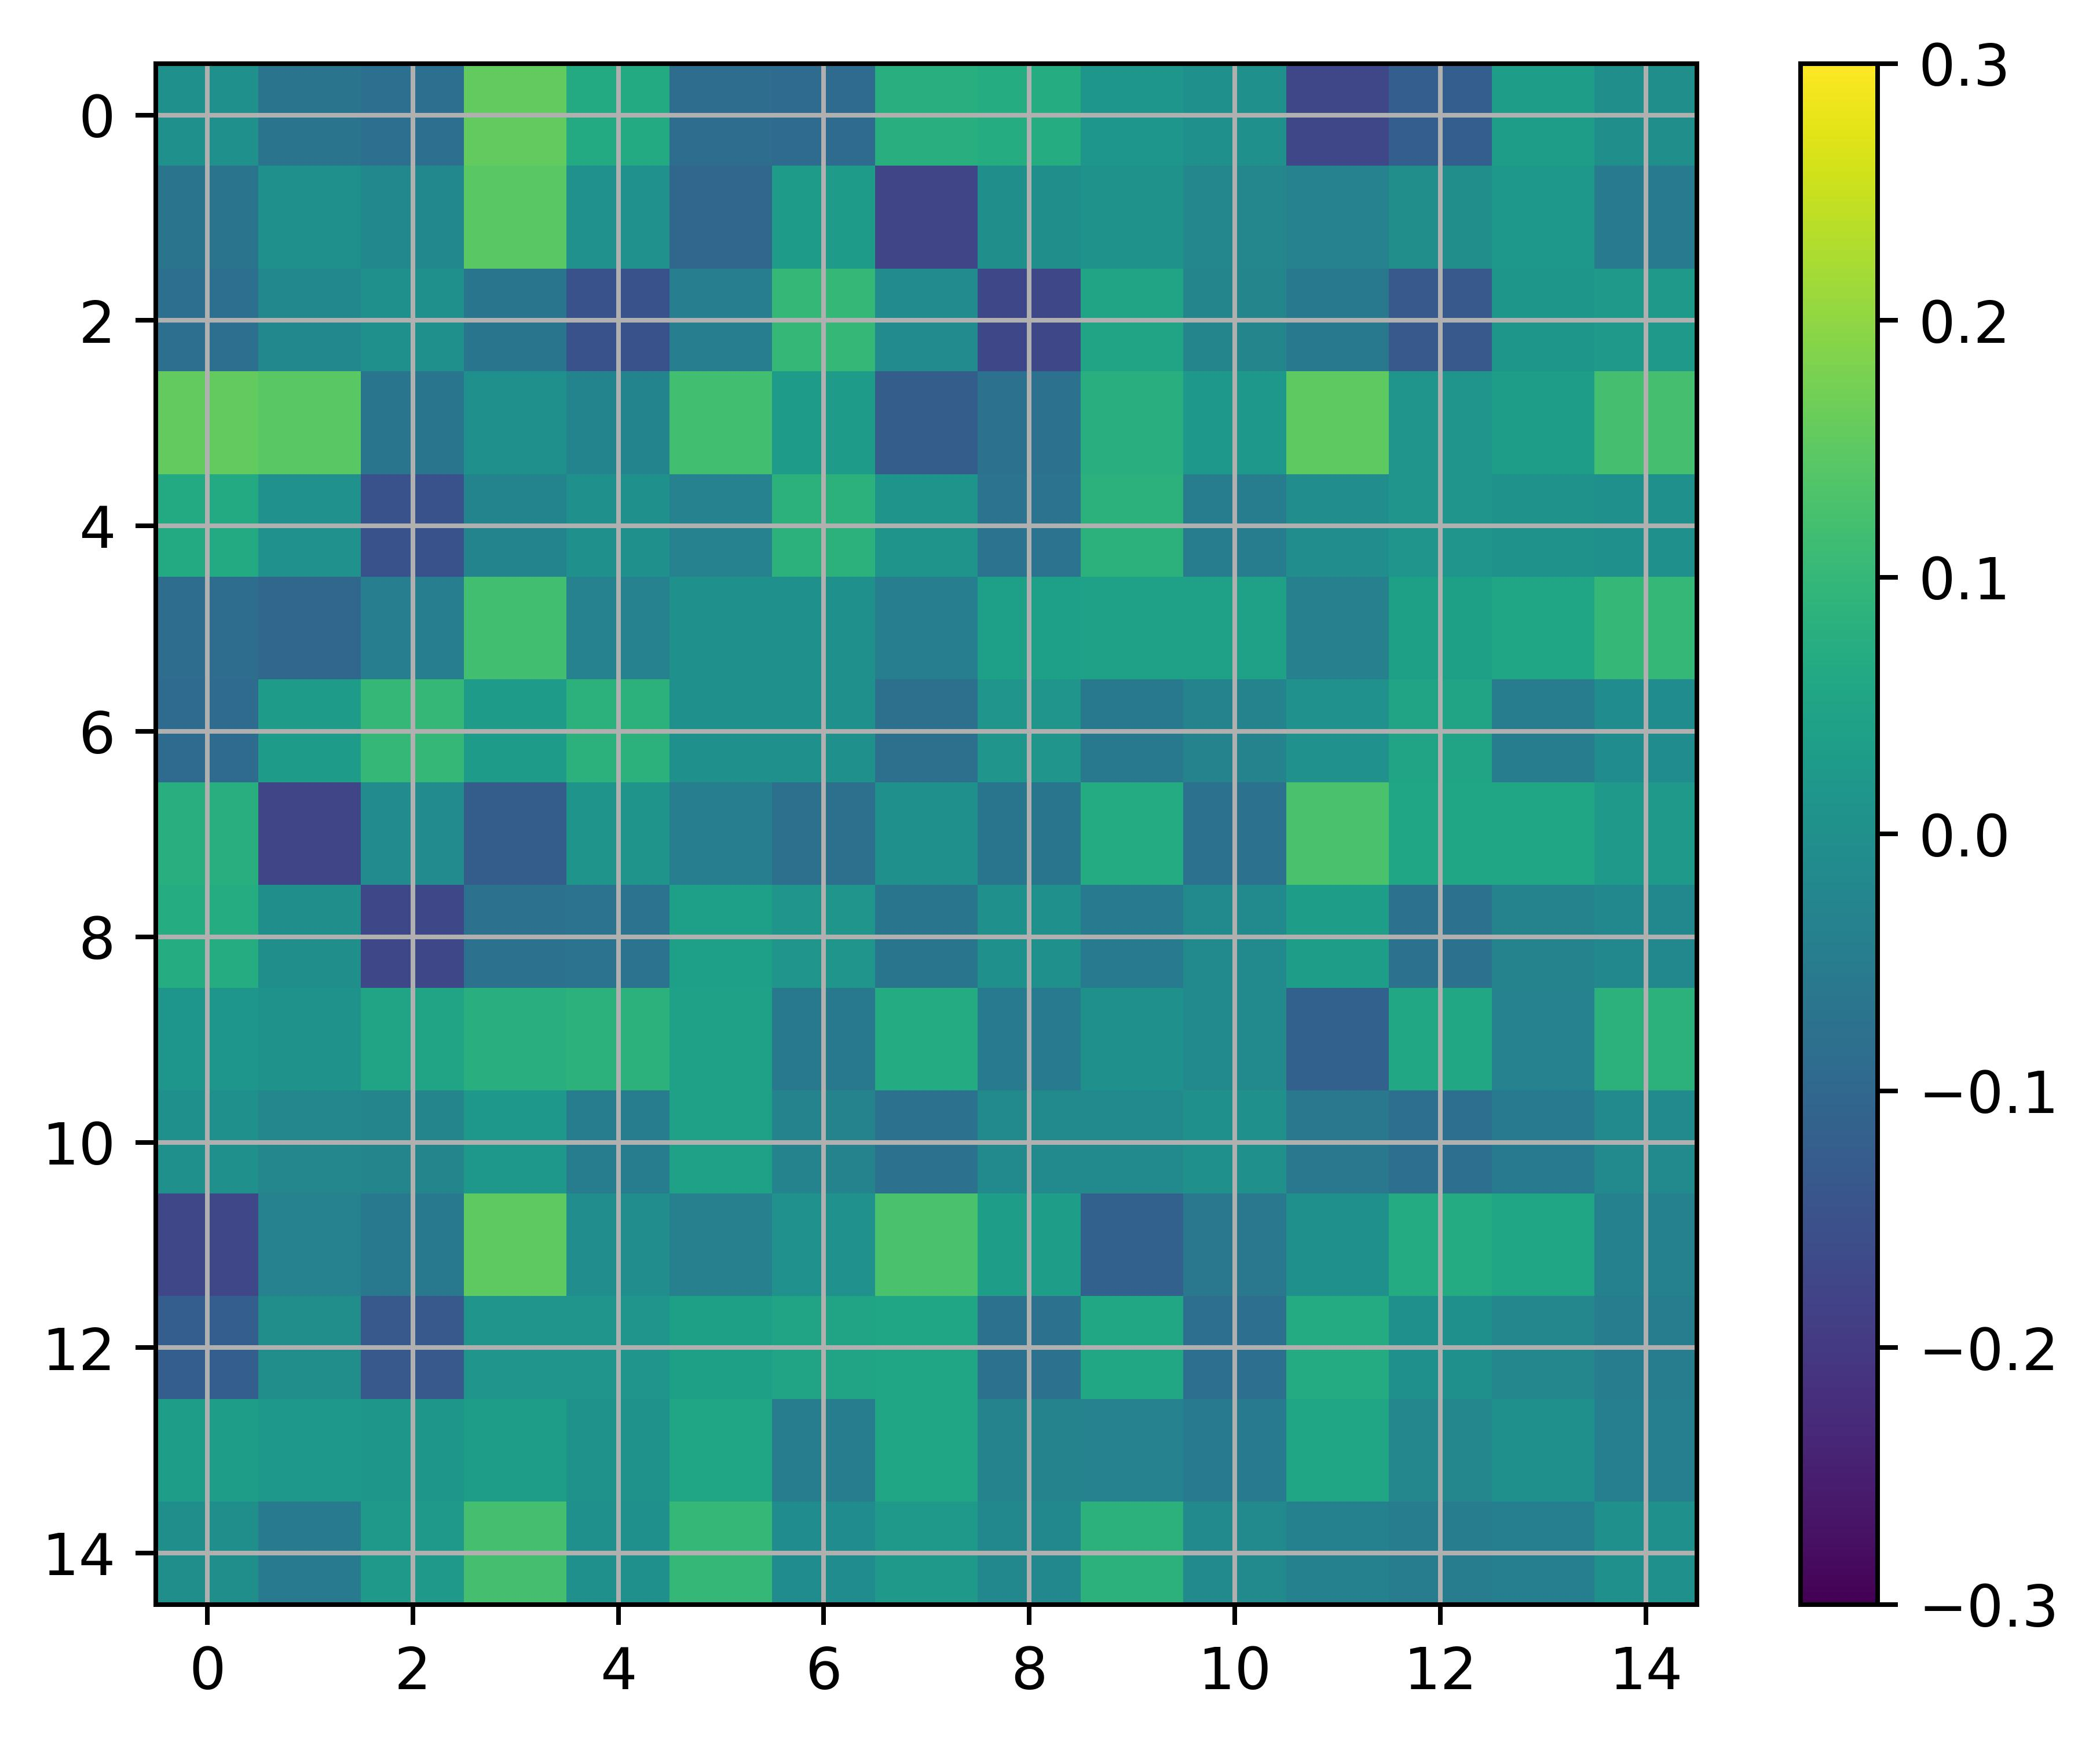
\includegraphics[width=0.2\textwidth]{../Analysis/DFC/size=480_step=180_rho=0.1/node=15_id=100206/c_4.jpg}
        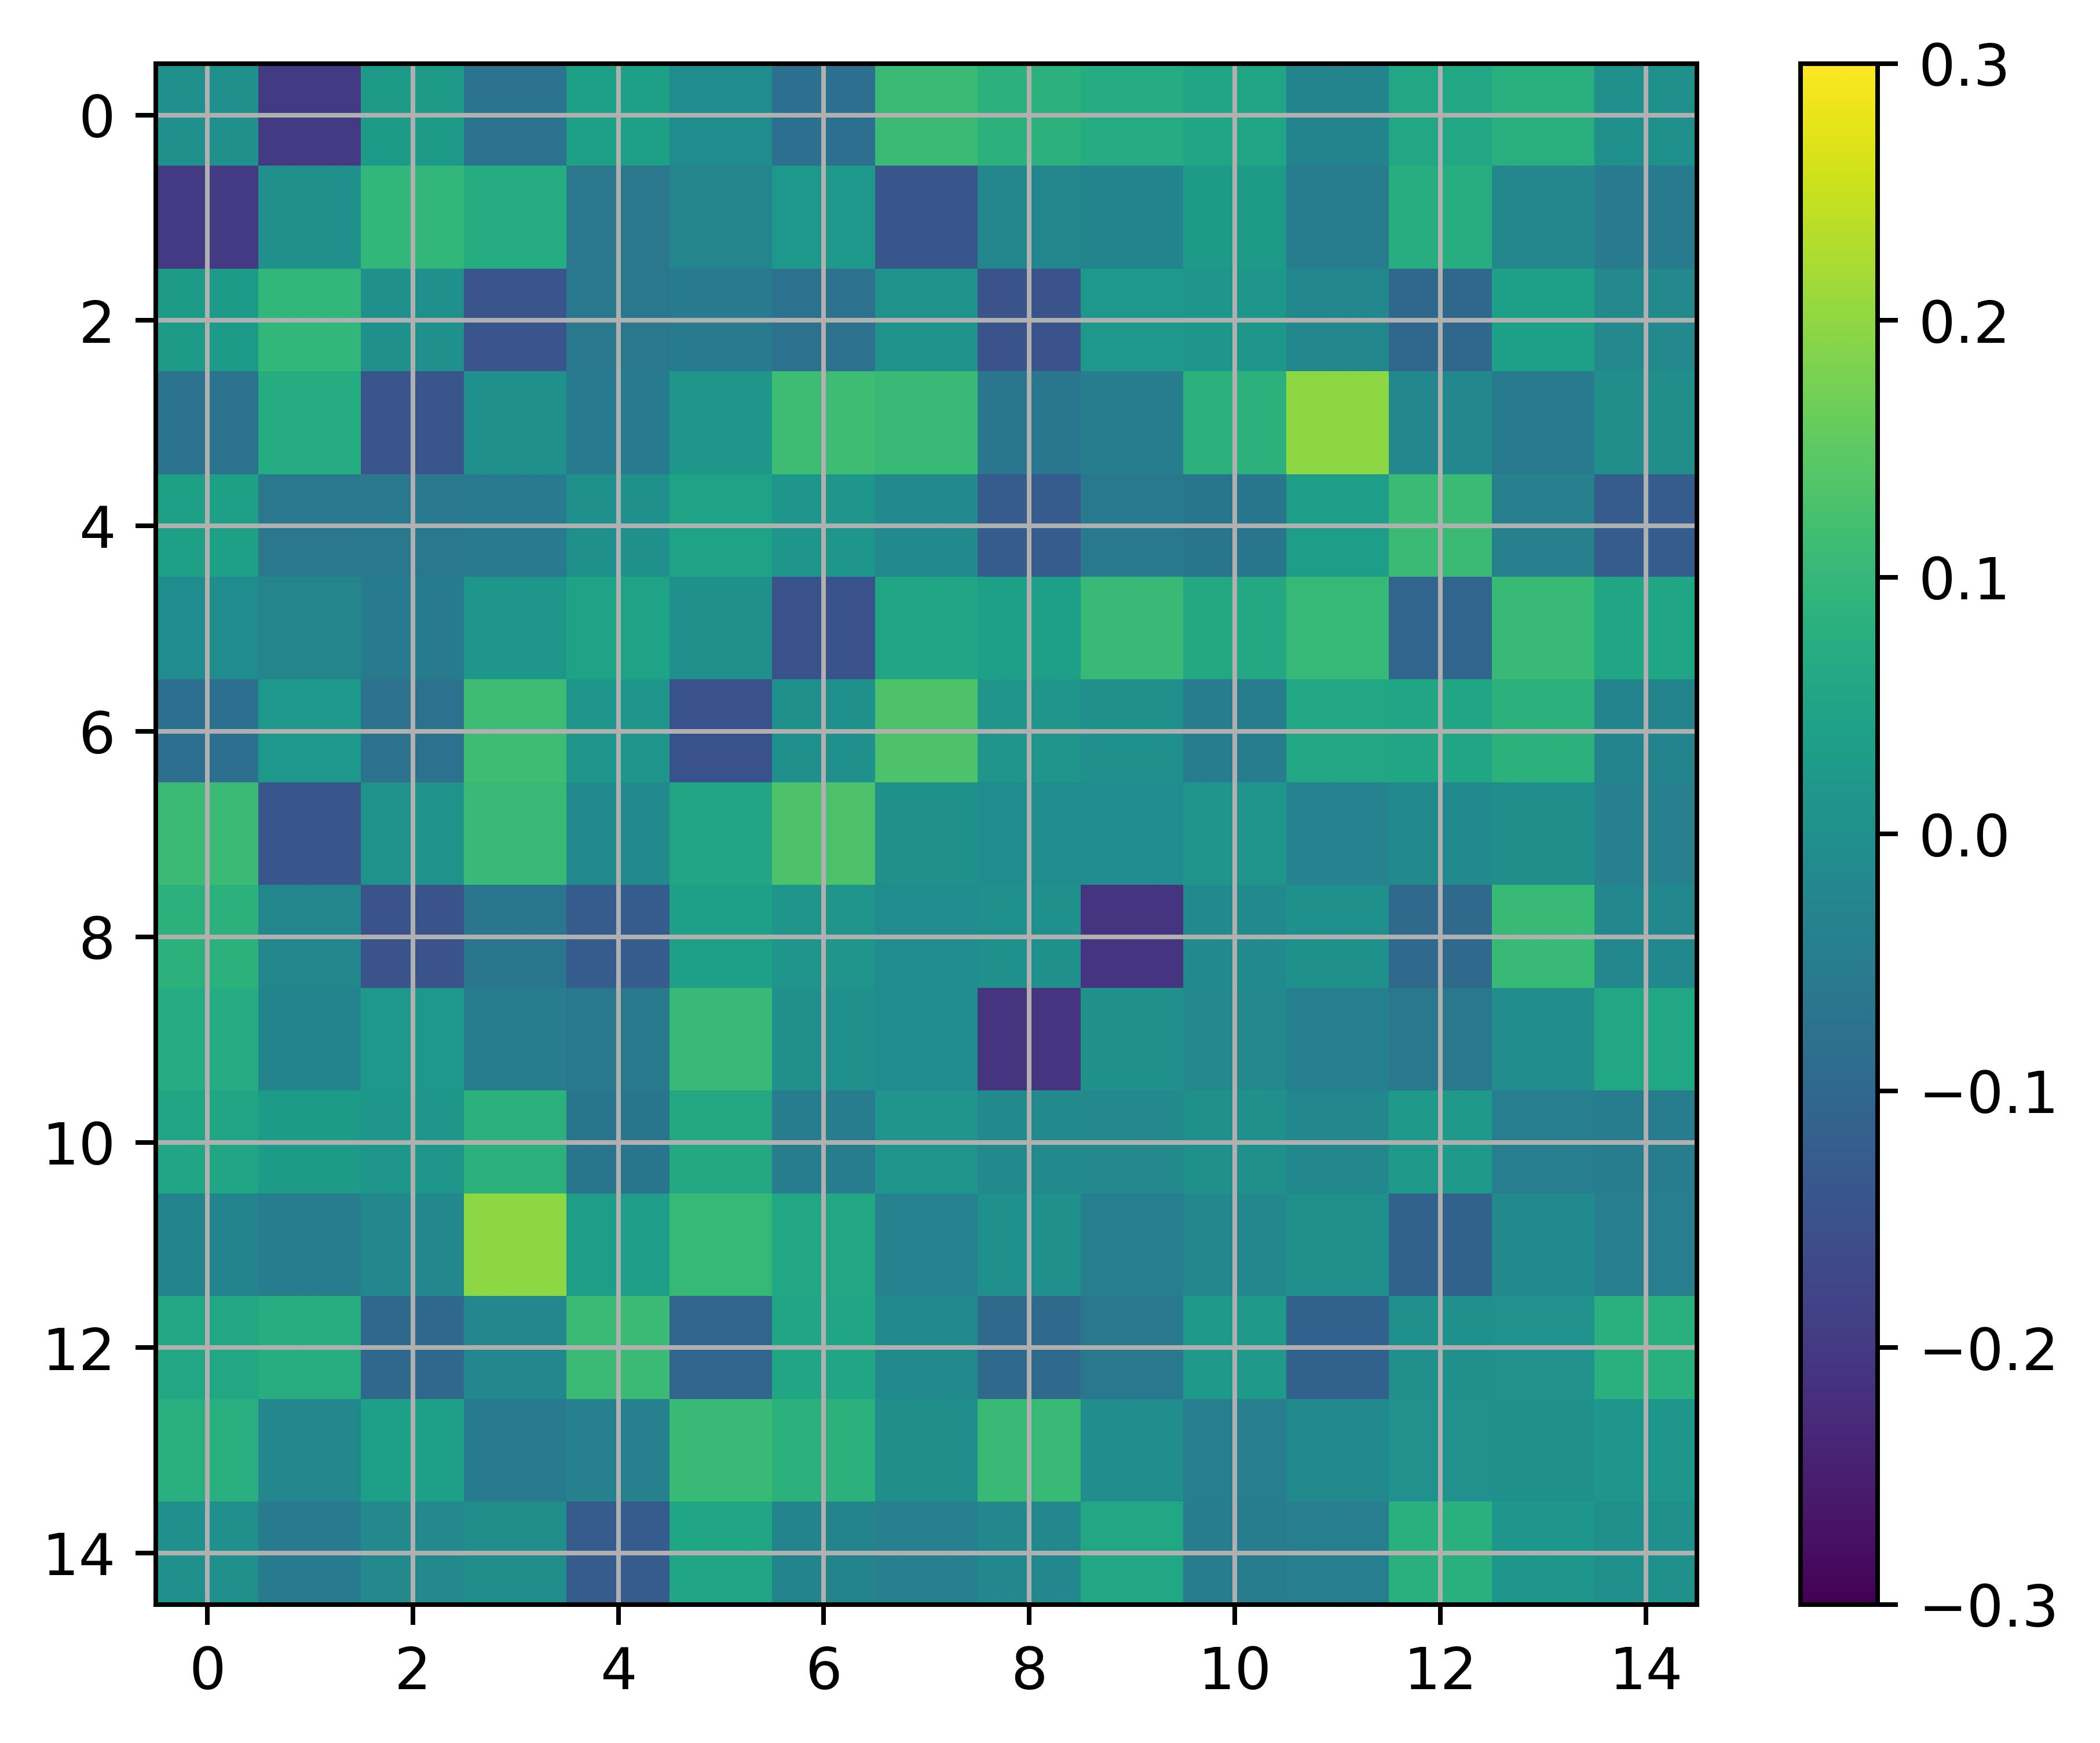
\includegraphics[width=0.2\textwidth]{../Analysis/DFC/size=480_step=180_rho=0.1/node=15_id=100206/c_6.jpg} \\
        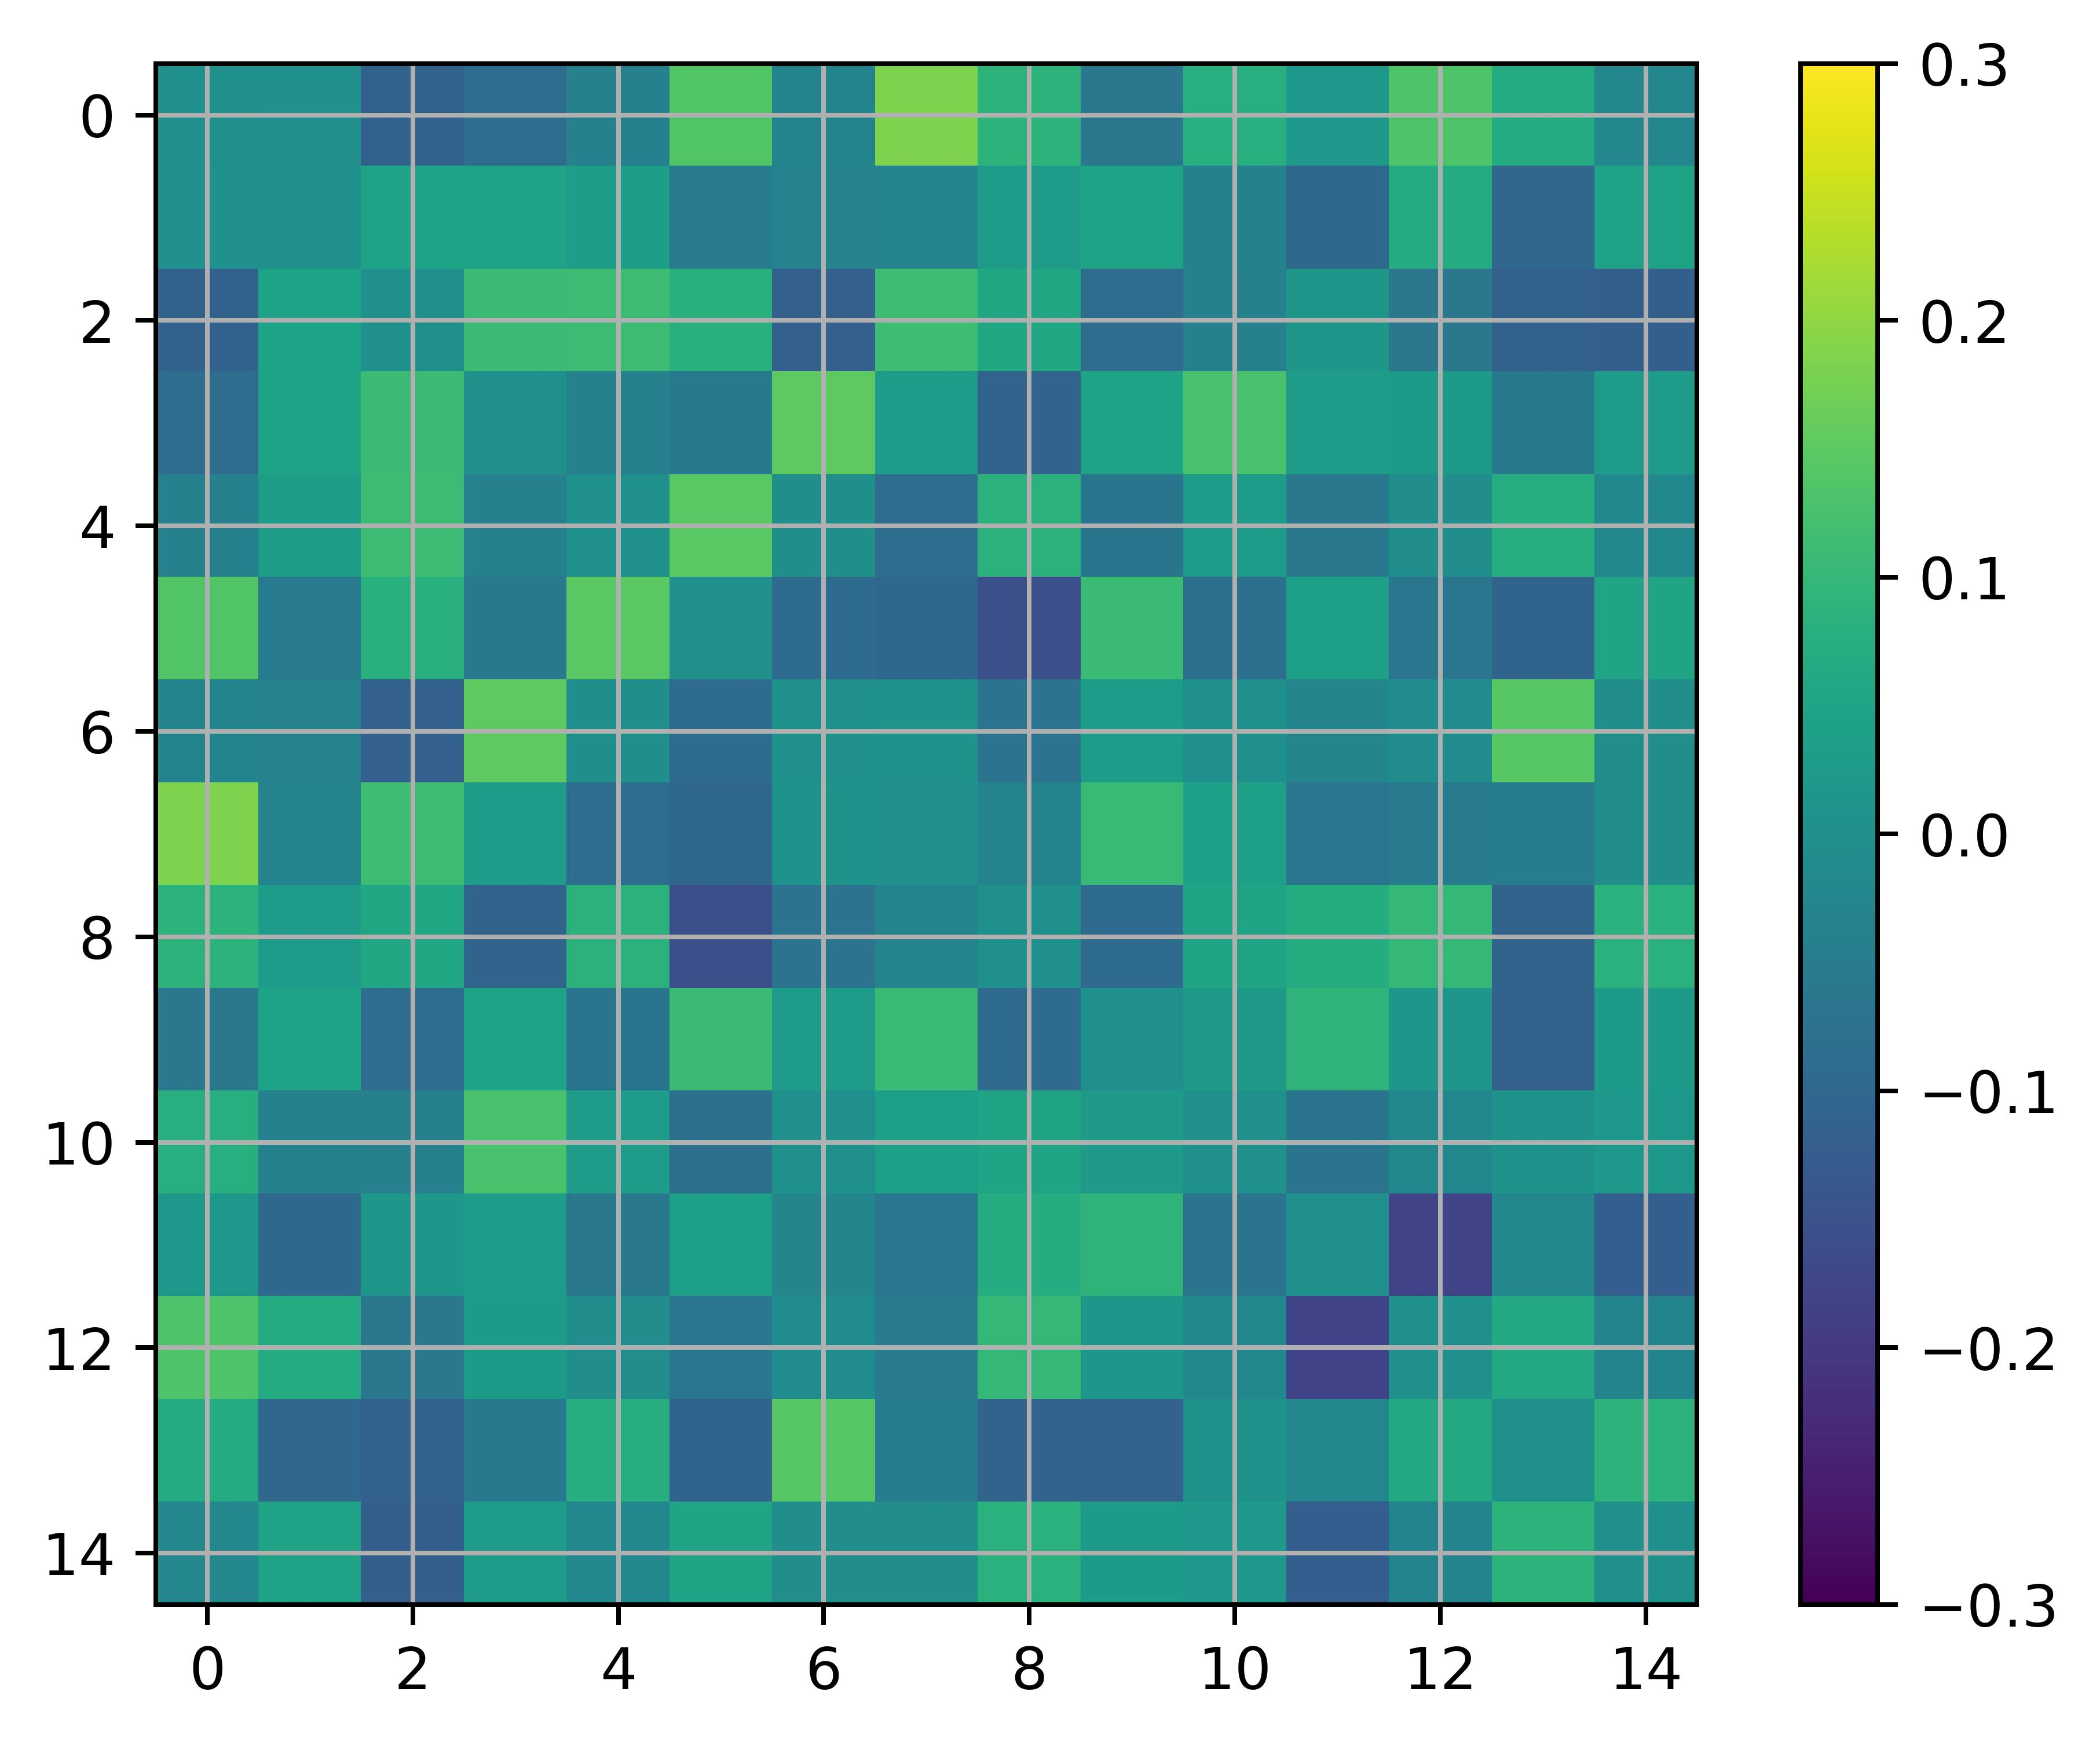
\includegraphics[width=0.2\textwidth]{../Analysis/DFC/size=480_step=180_rho=0.1/node=15_id=100206/c_8.jpg}
        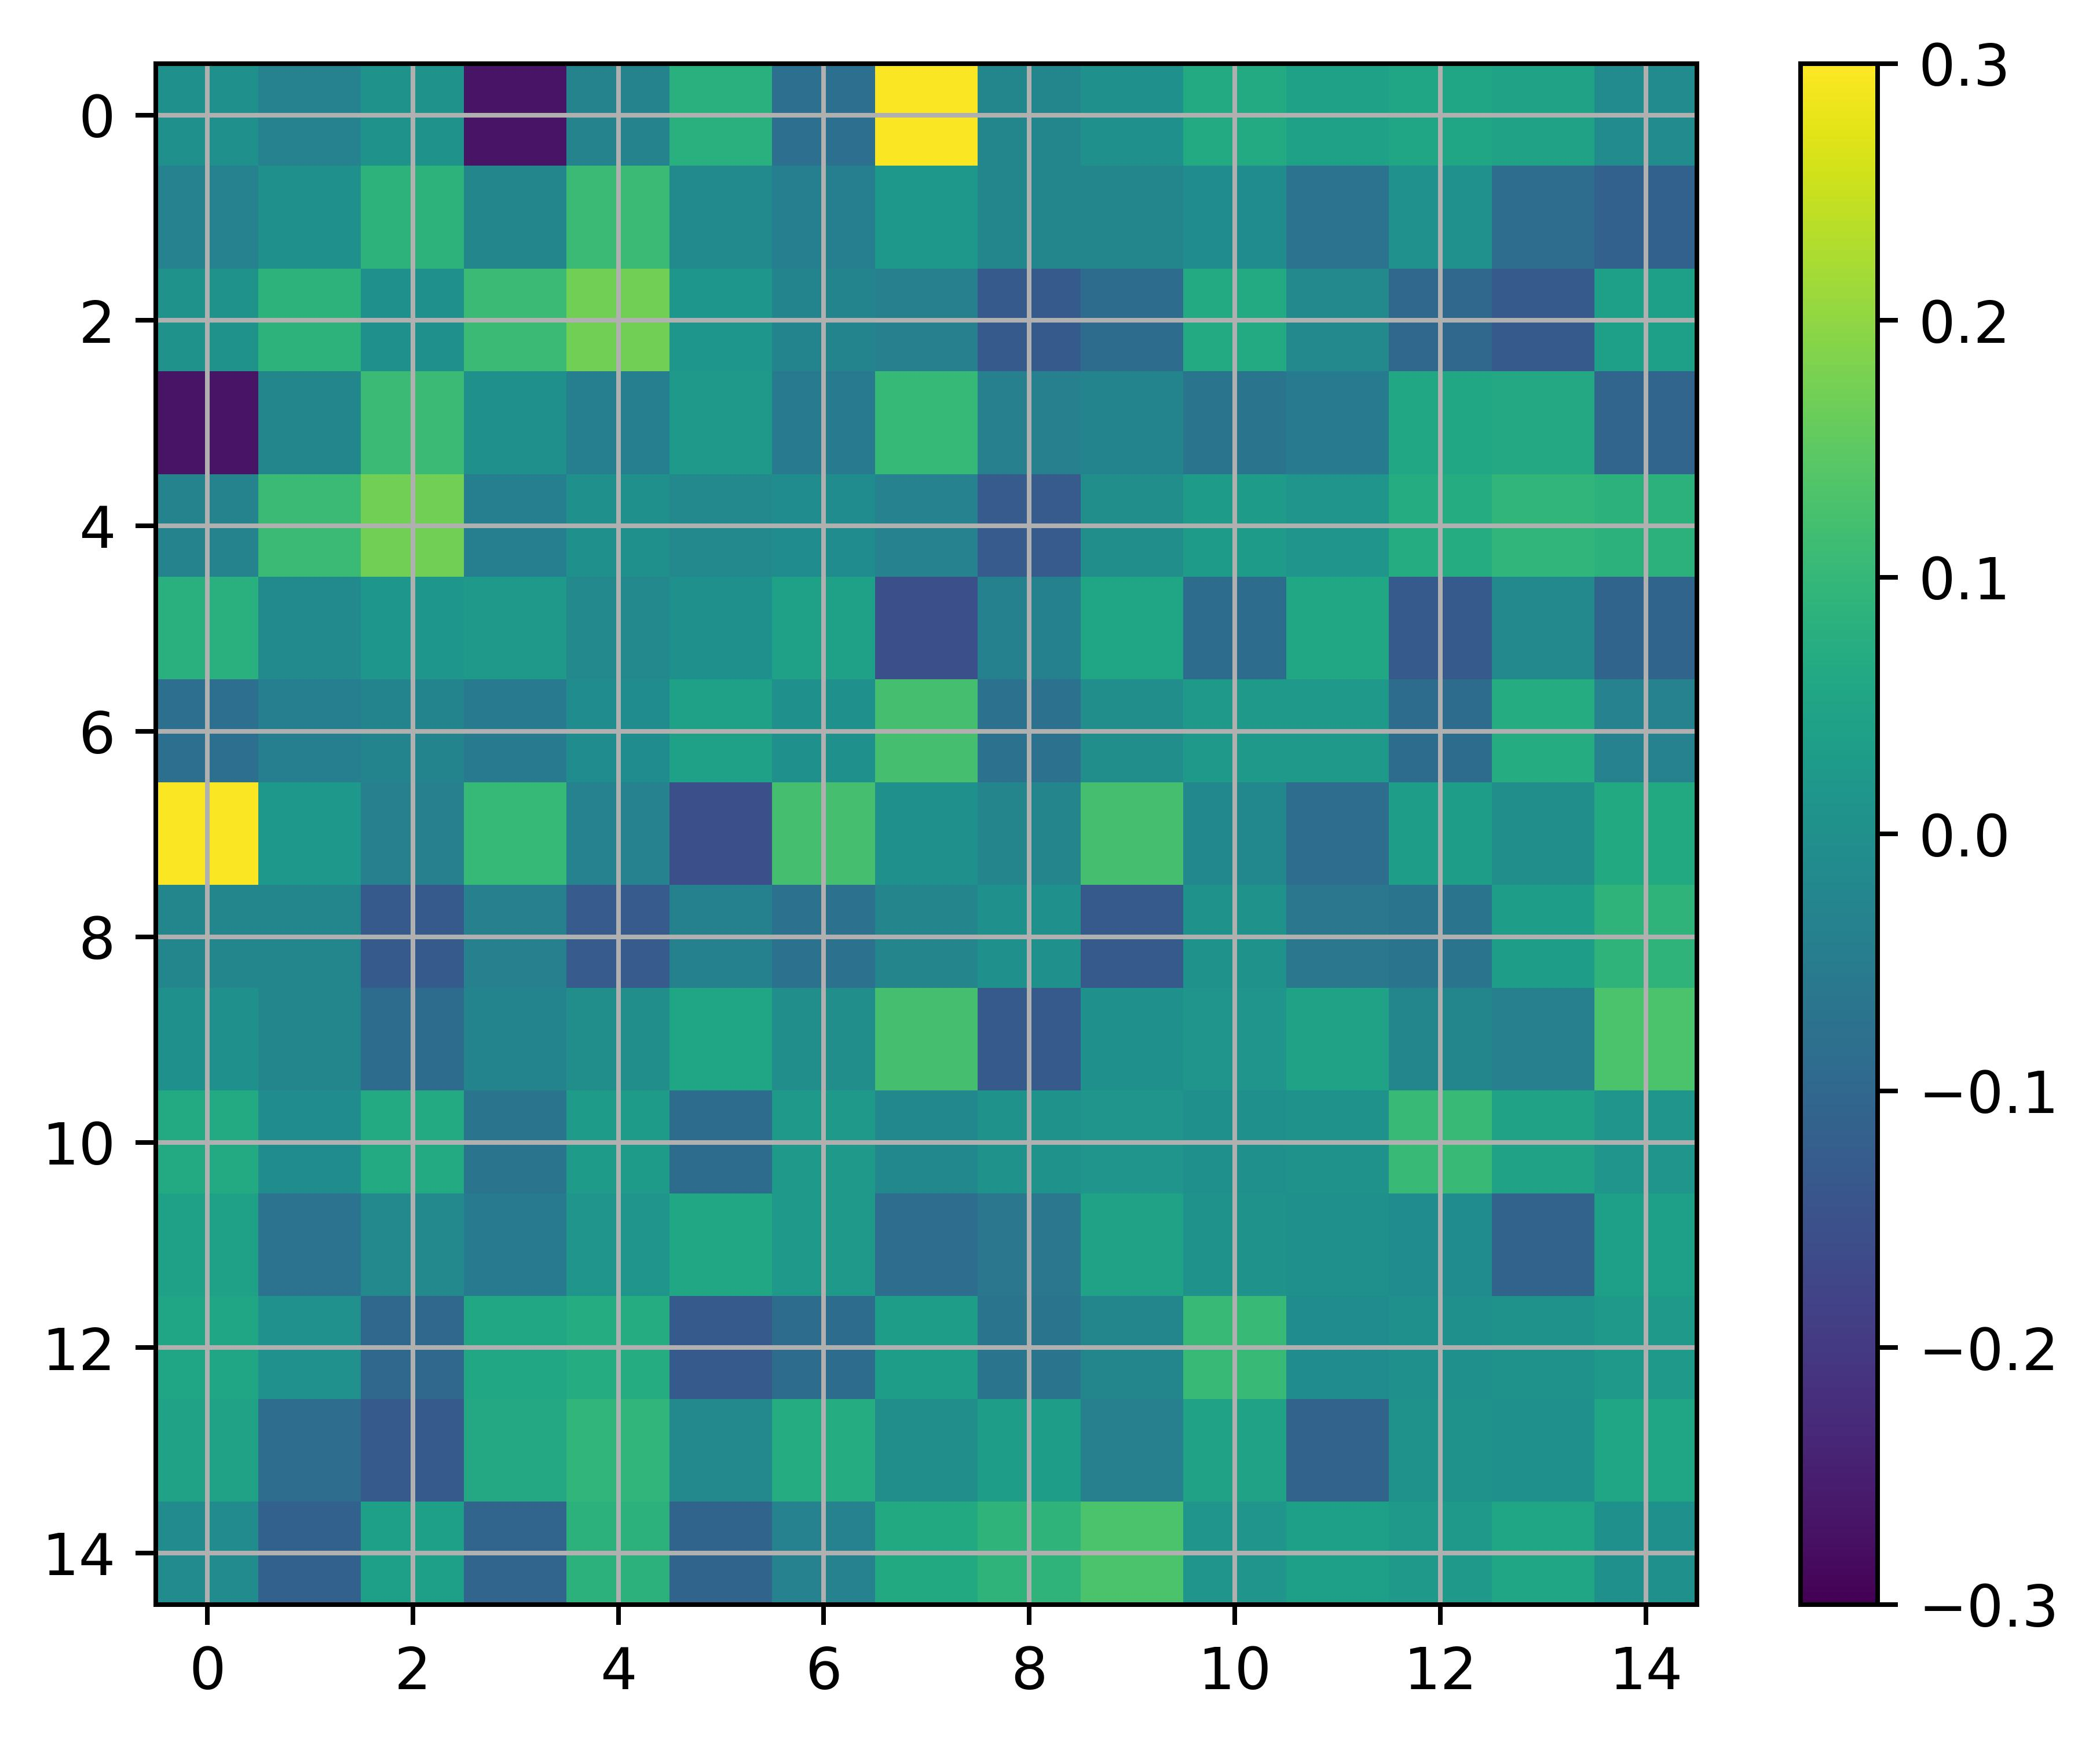
\includegraphics[width=0.2\textwidth]{../Analysis/DFC/size=480_step=180_rho=0.1/node=15_id=100206/c_10.jpg}
        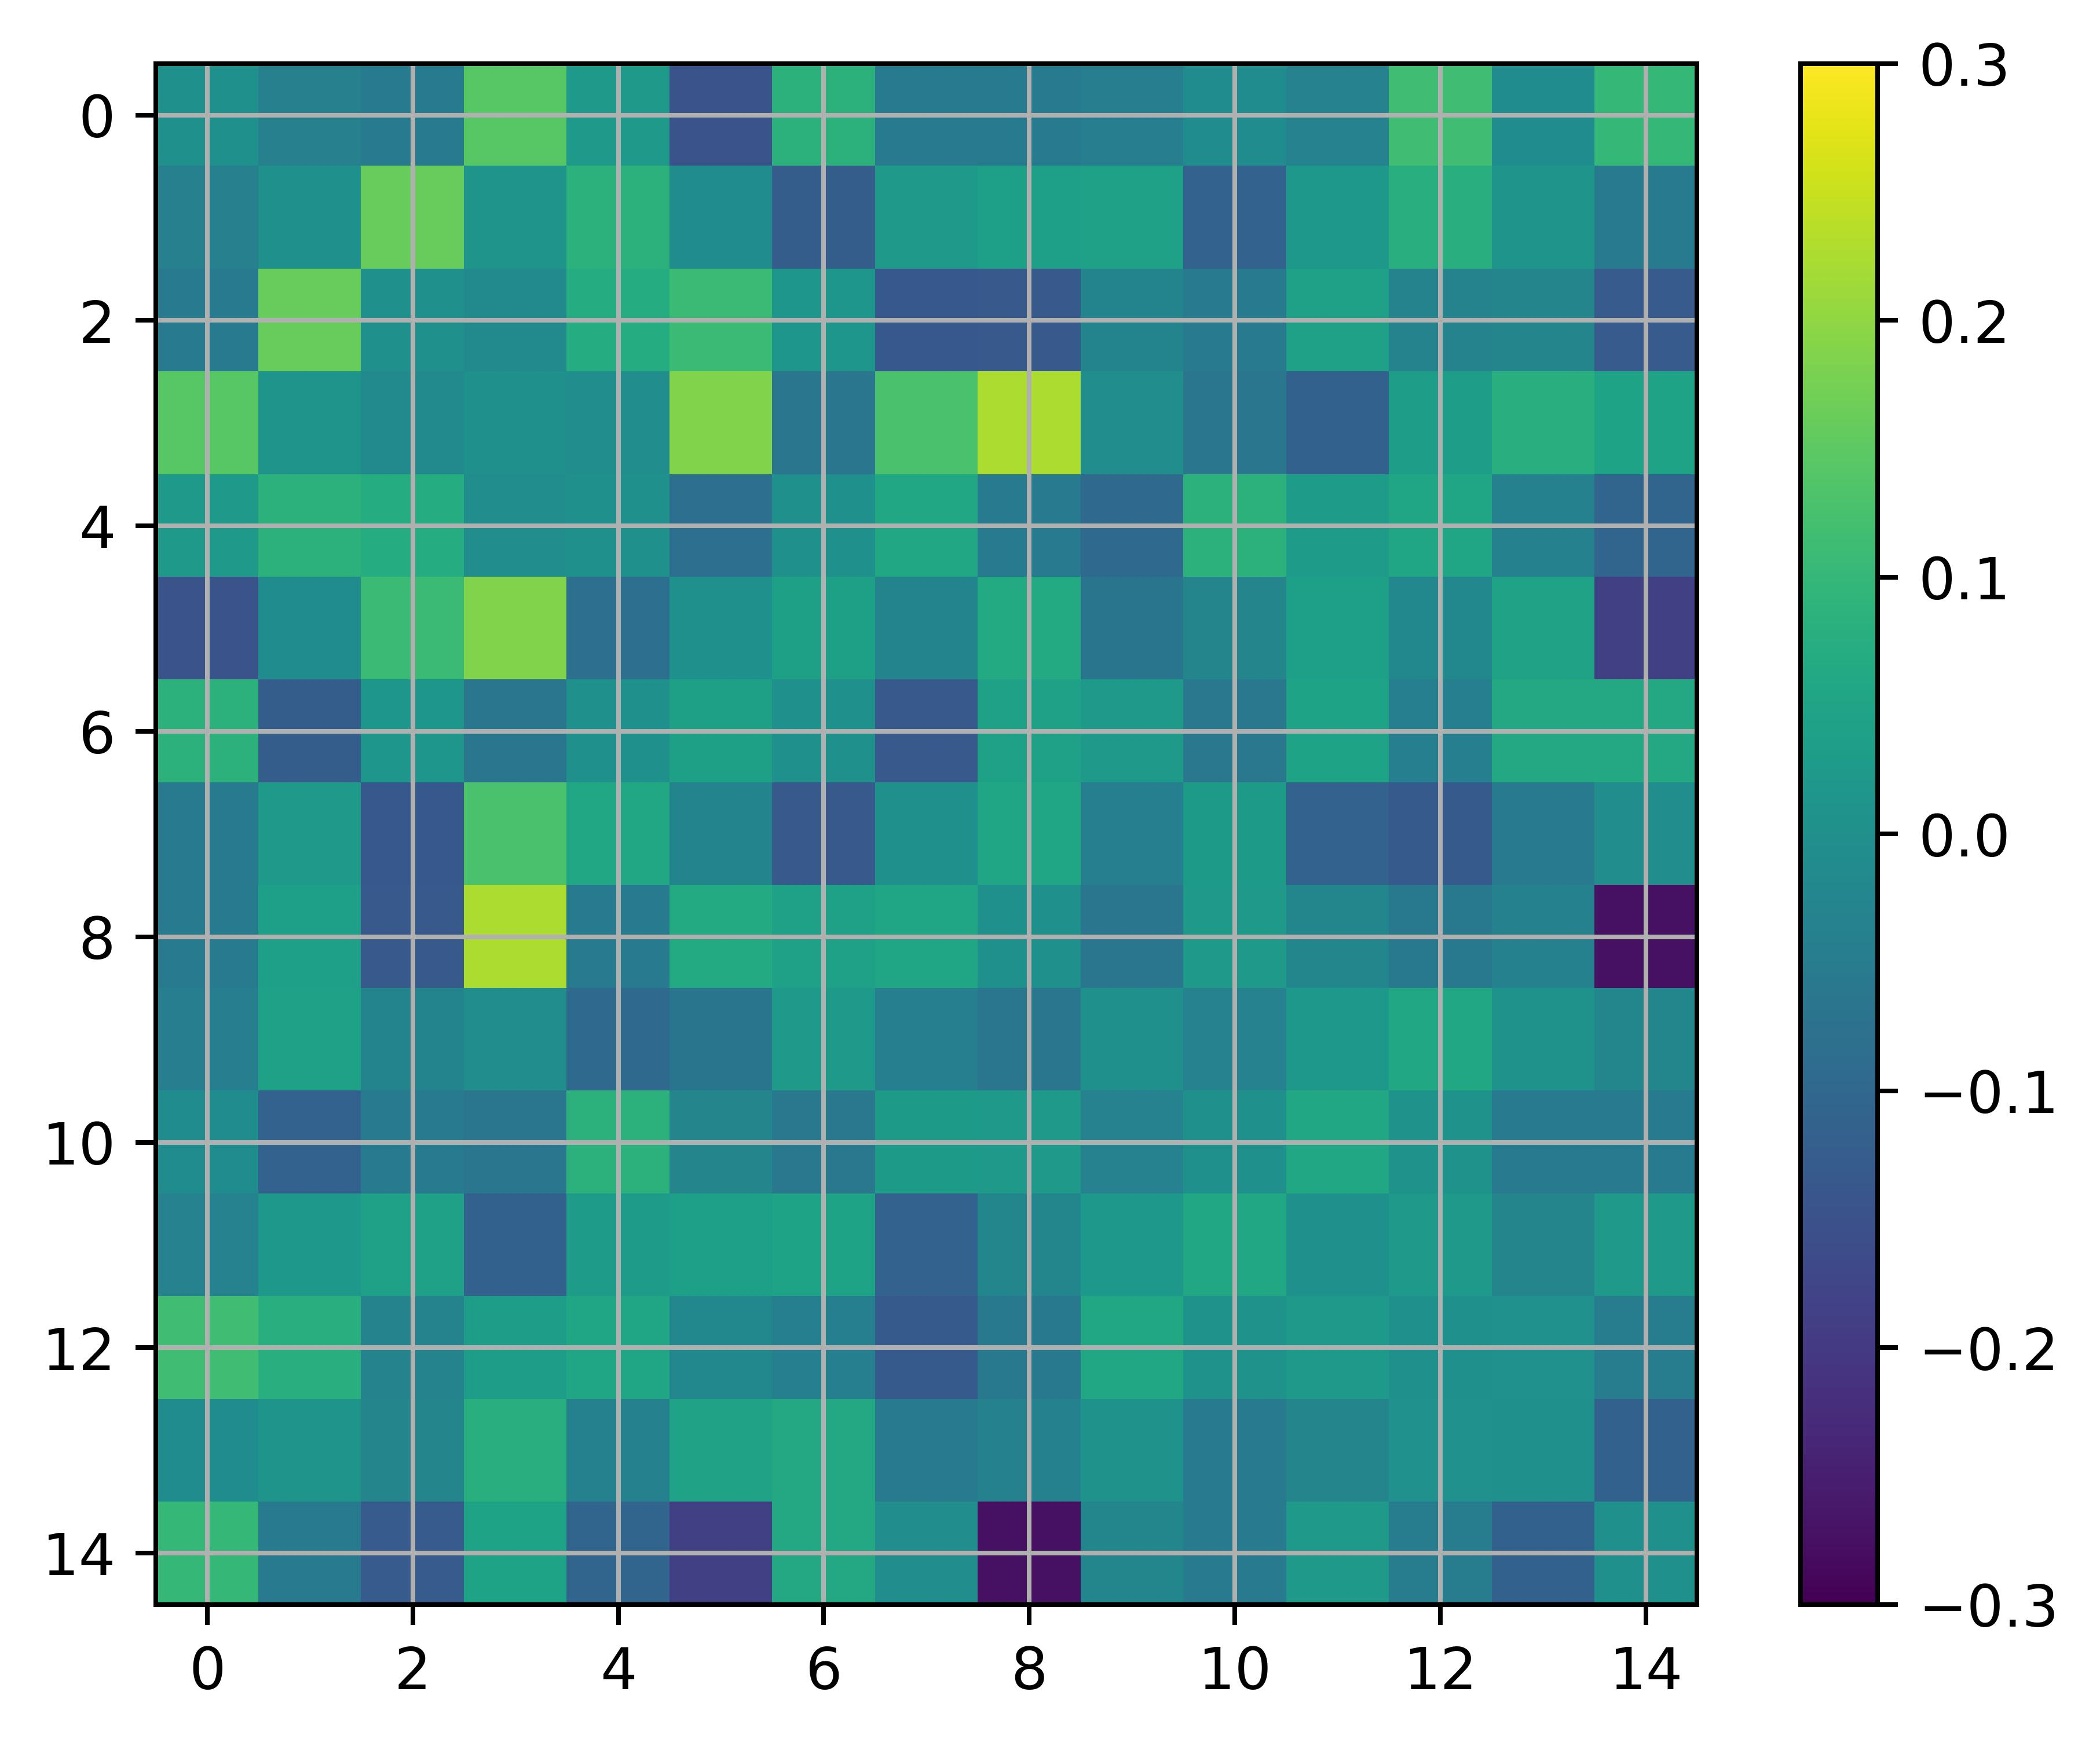
\includegraphics[width=0.2\textwidth]{../Analysis/DFC/size=480_step=180_rho=0.1/node=15_id=100206/c_12.jpg}
        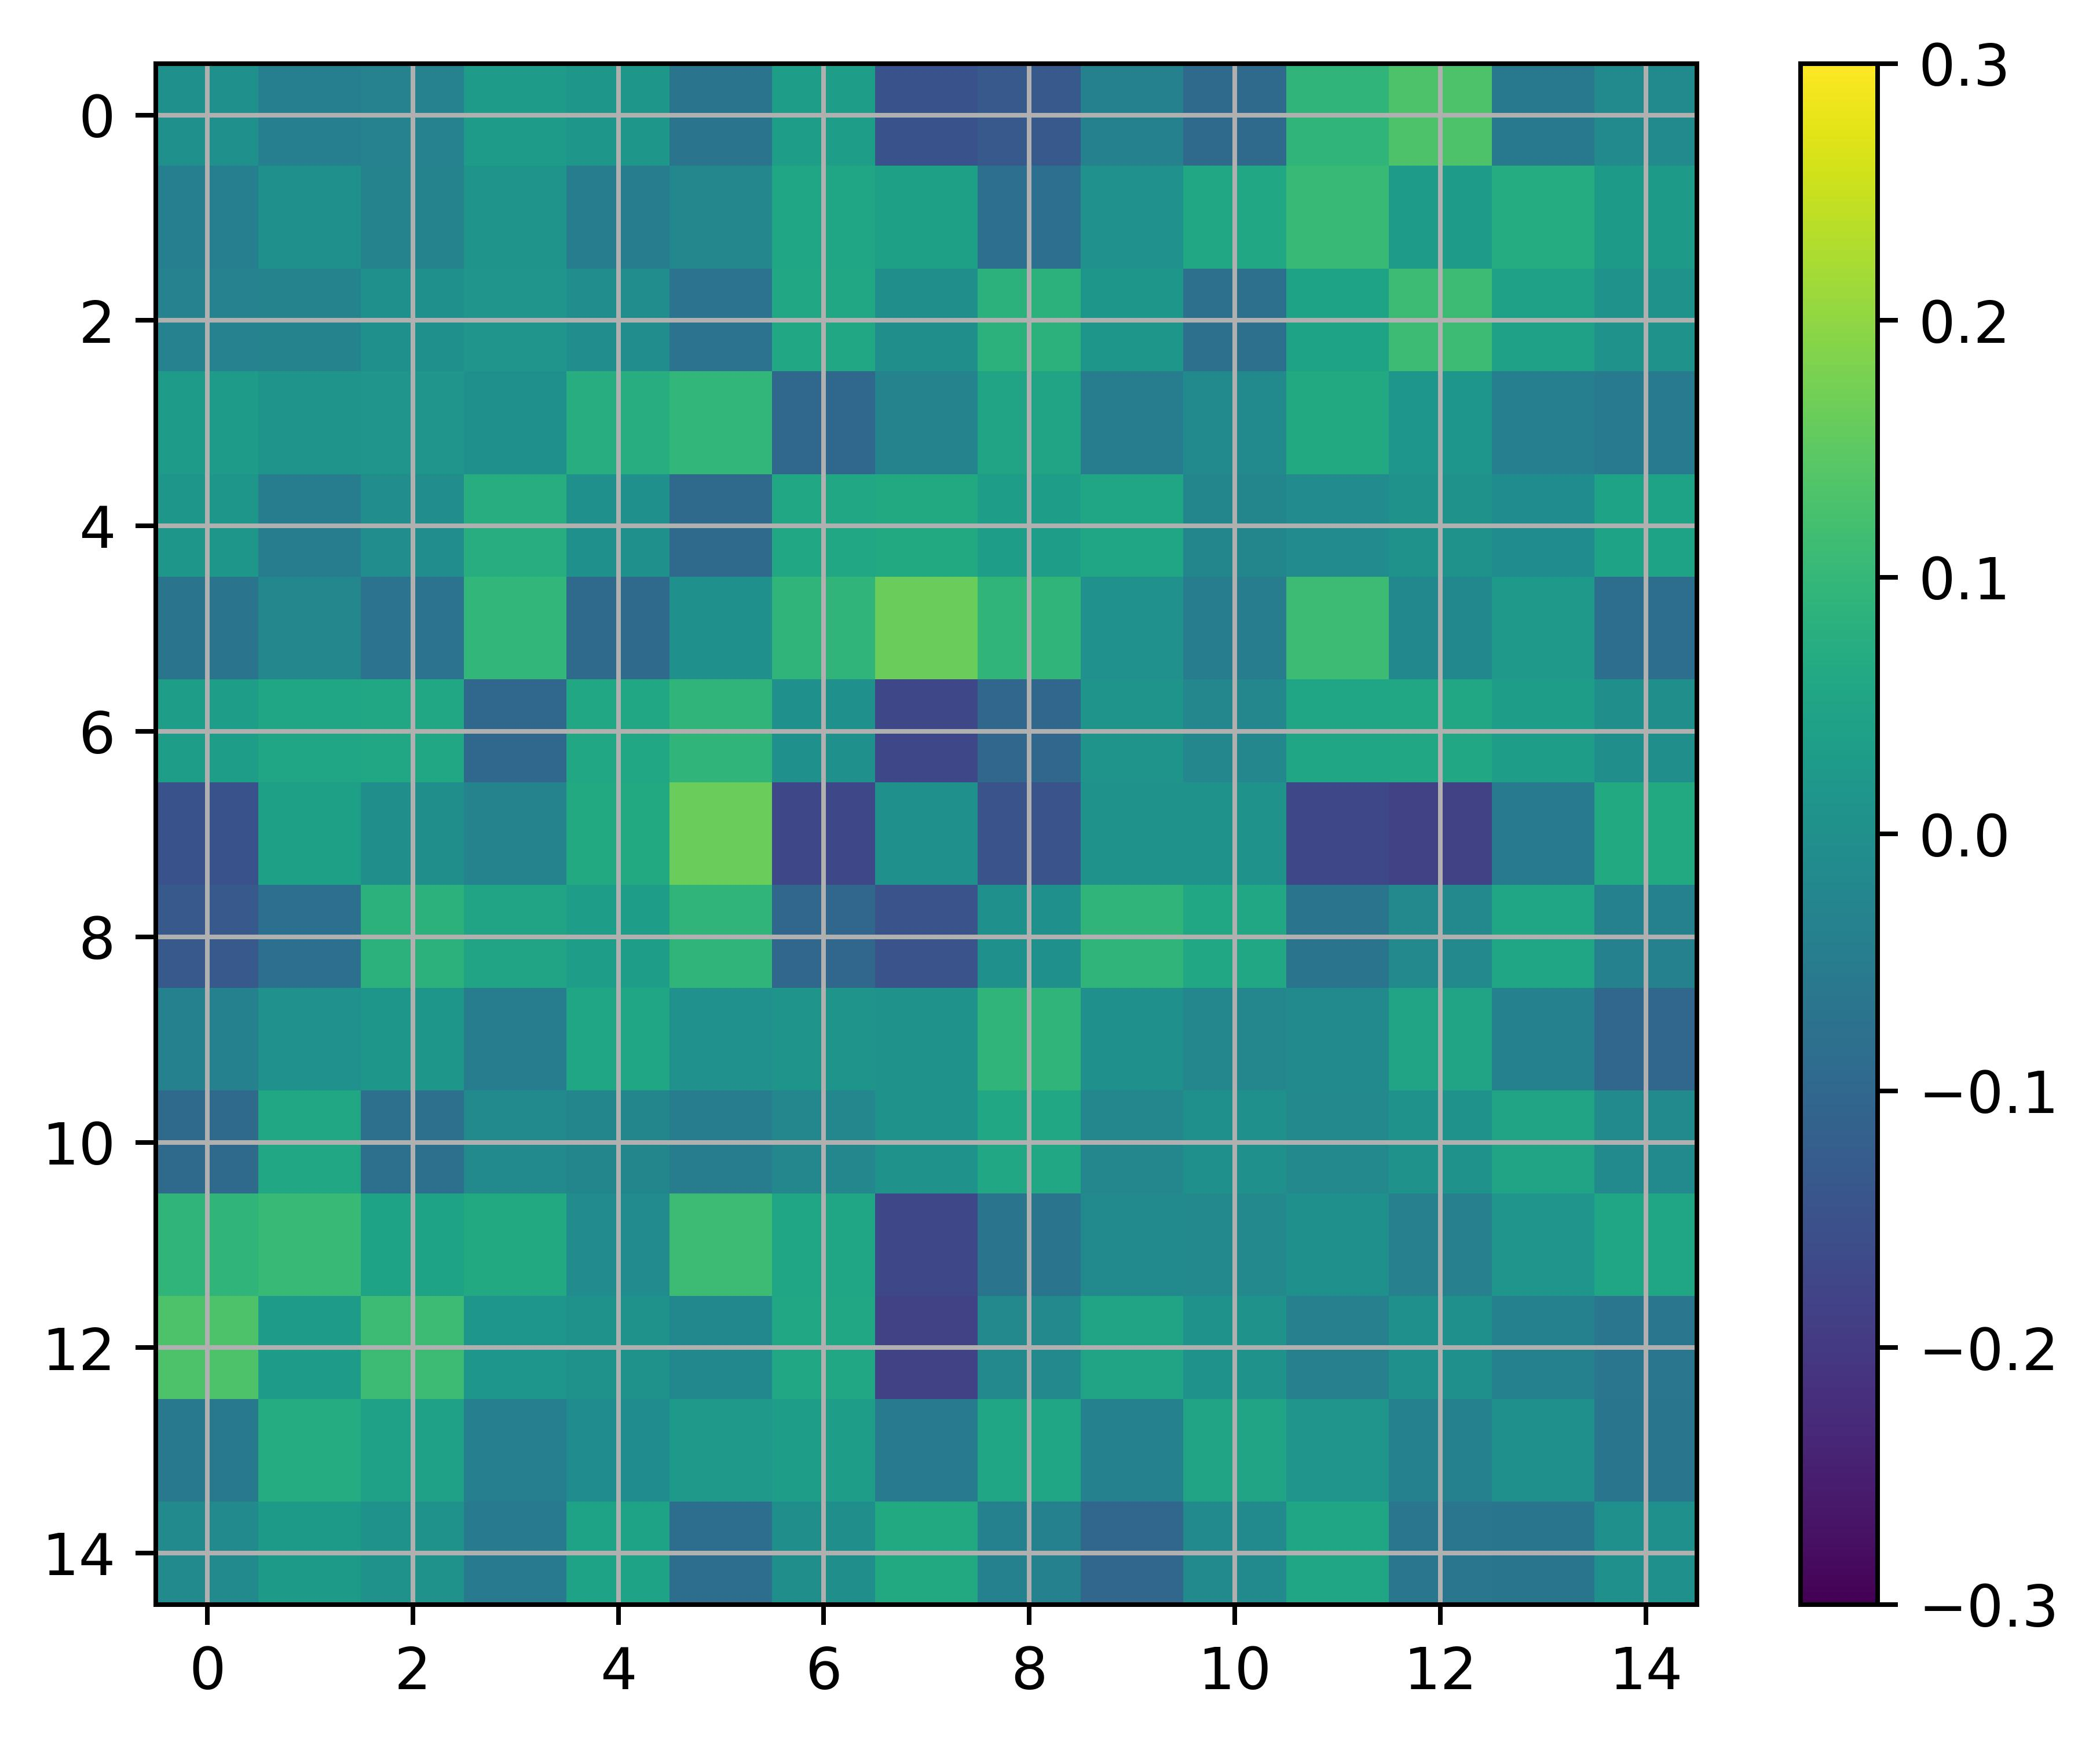
\includegraphics[width=0.2\textwidth]{../Analysis/DFC/size=480_step=180_rho=0.1/node=15_id=100206/c_14.jpg} \\
        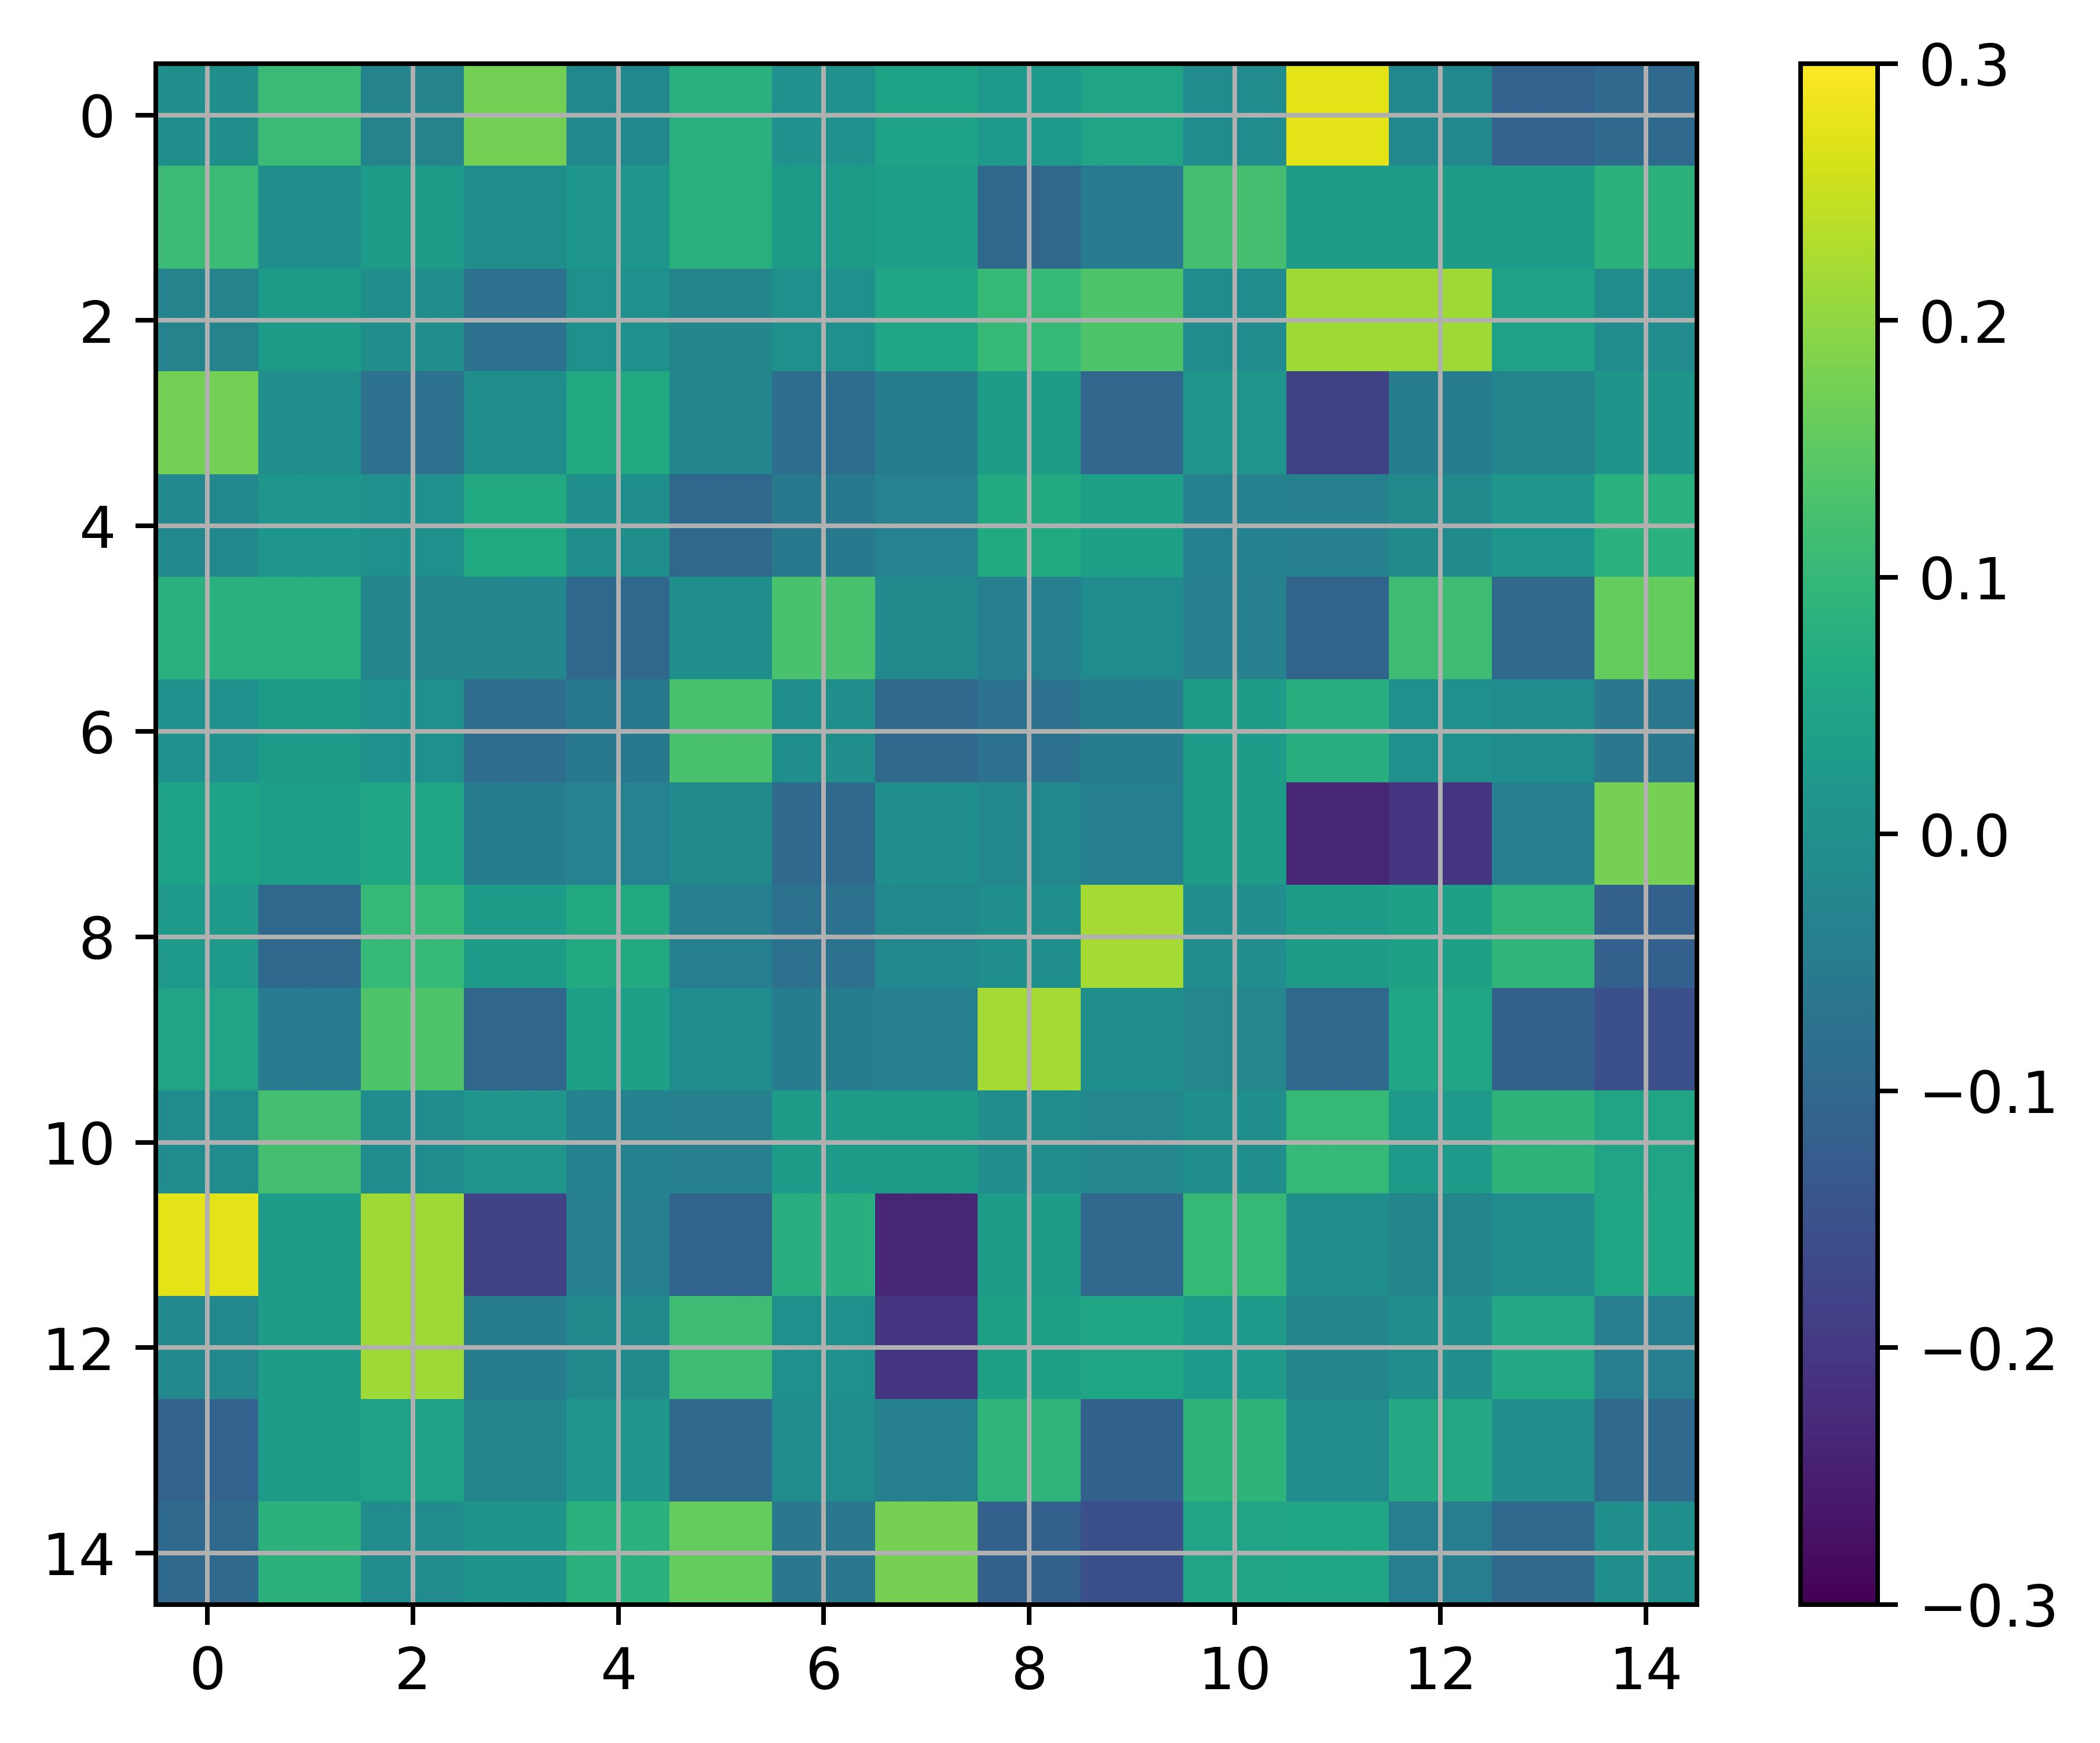
\includegraphics[width=0.2\textwidth]{../Analysis/DFC/size=480_step=180_rho=0.1/node=15_id=100206/c_16.jpg}
        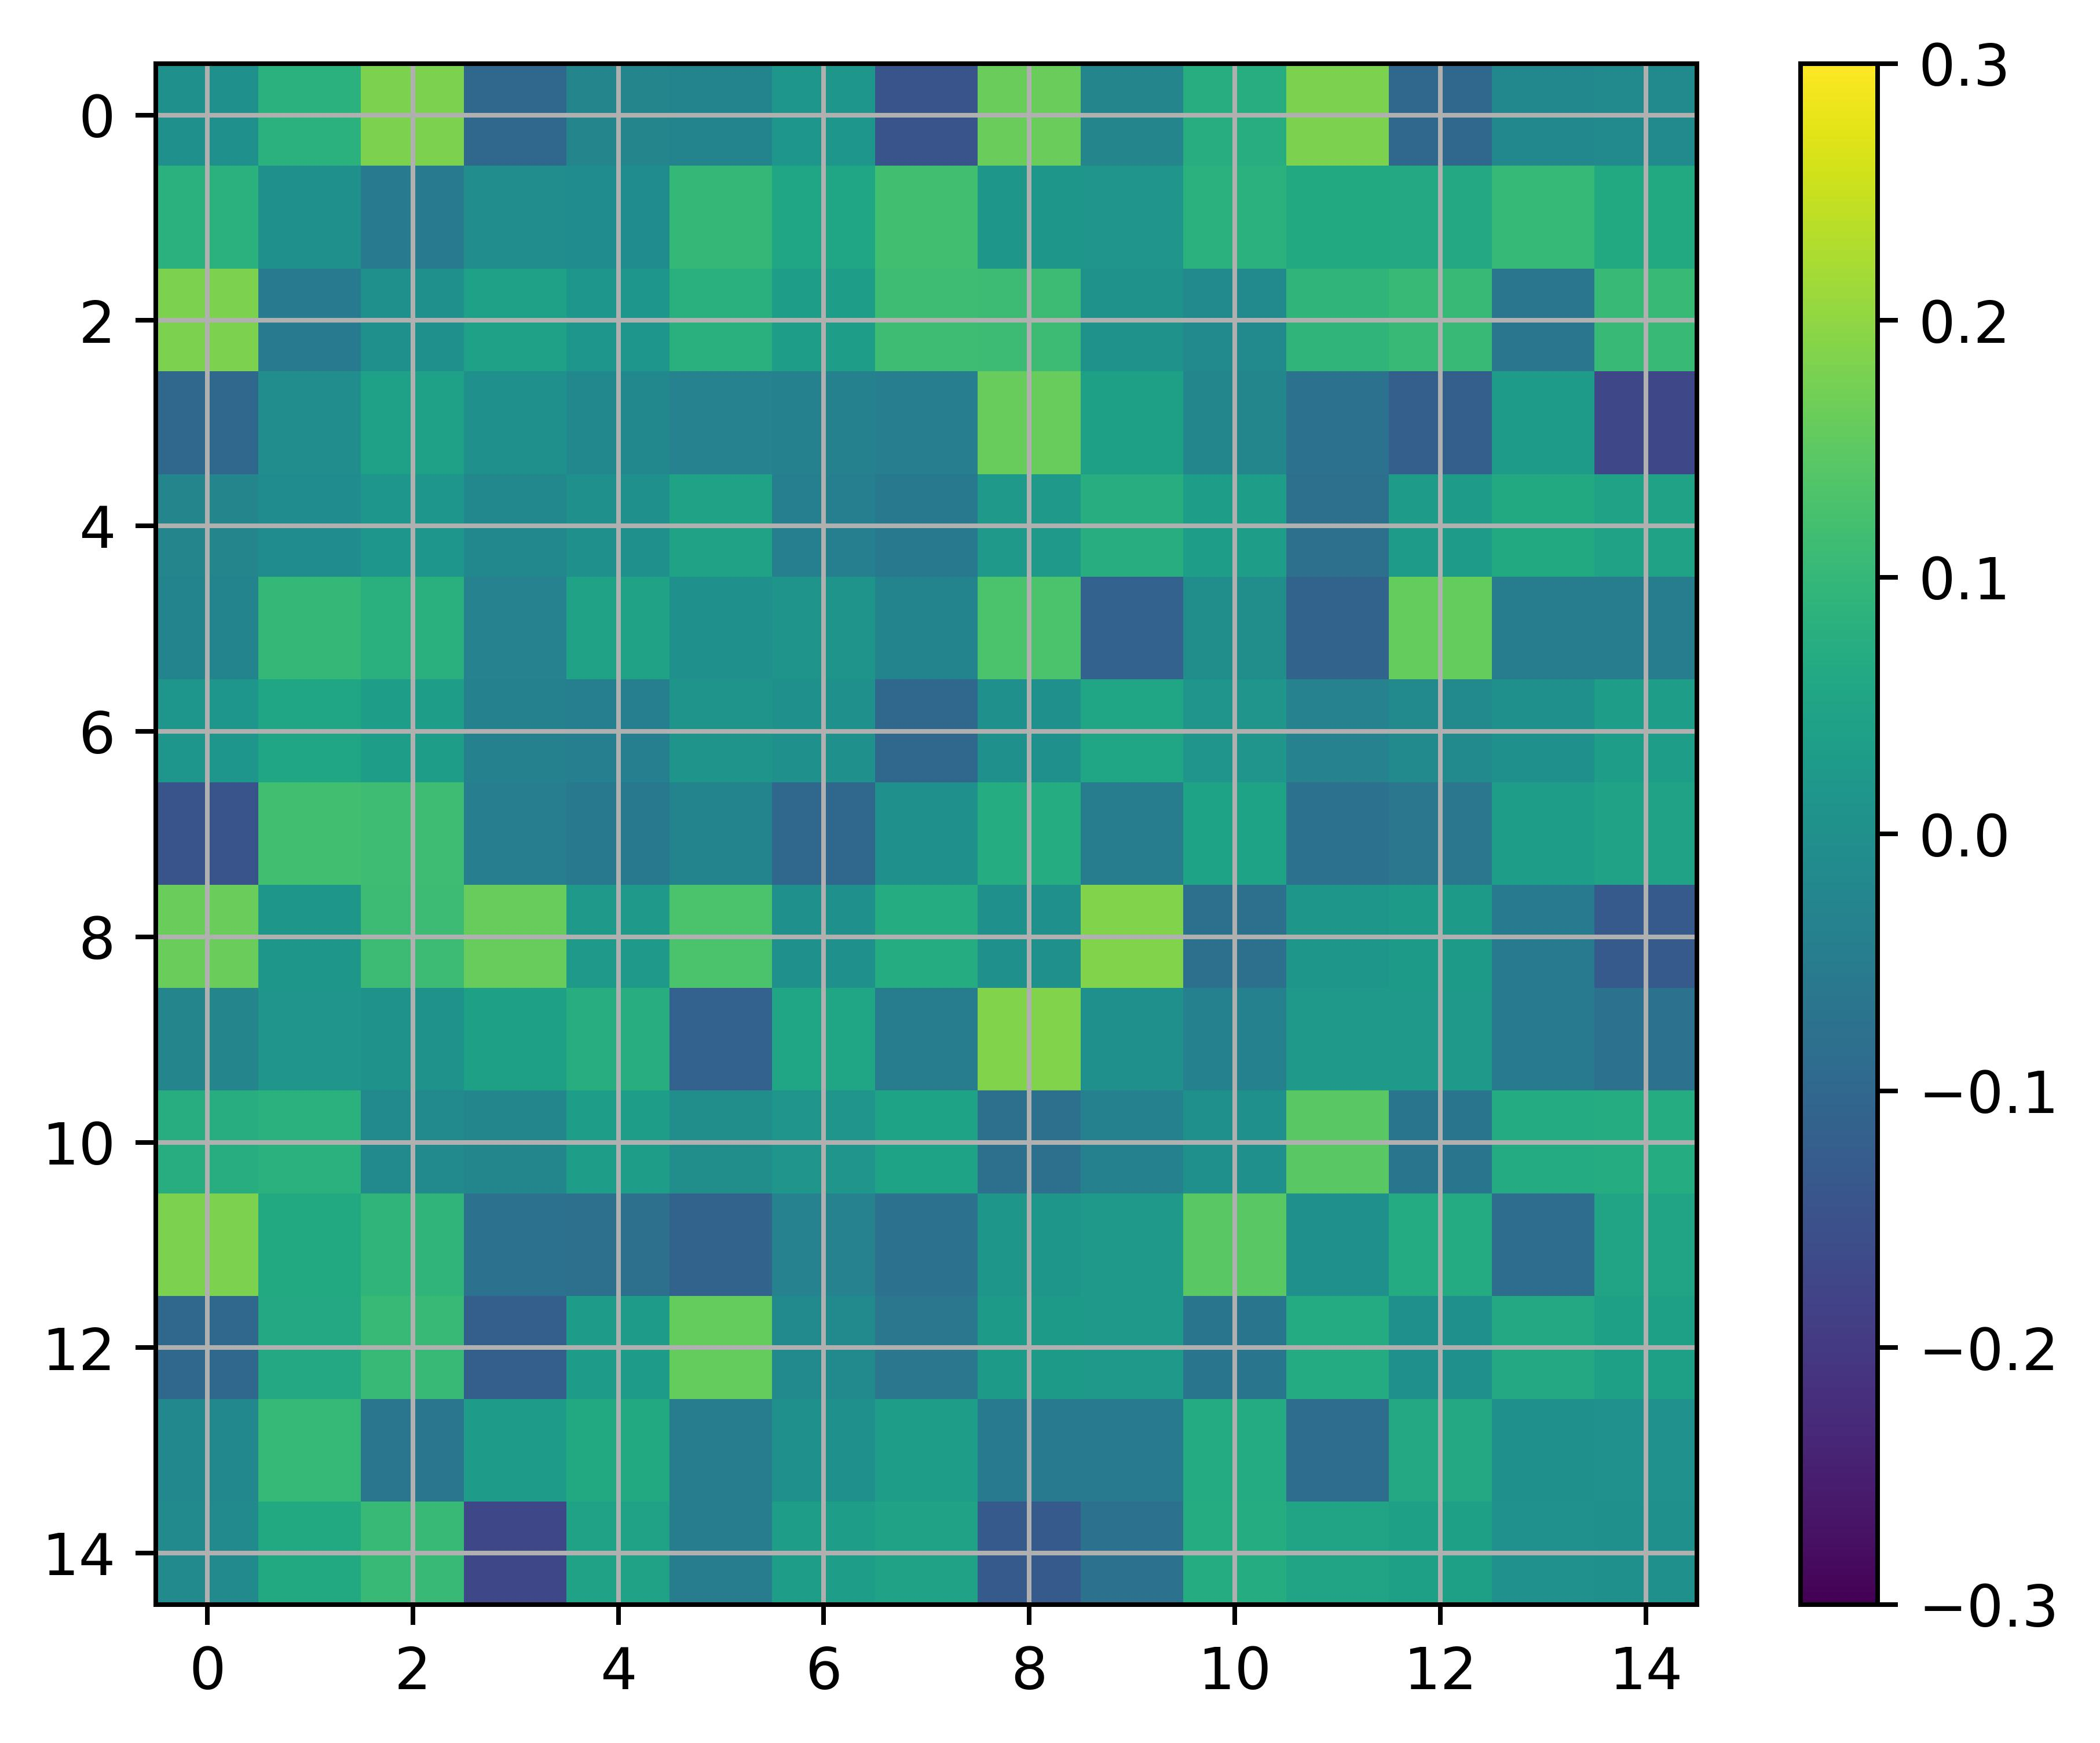
\includegraphics[width=0.2\textwidth]{../Analysis/DFC/size=480_step=180_rho=0.1/node=15_id=100206/c_18.jpg}
        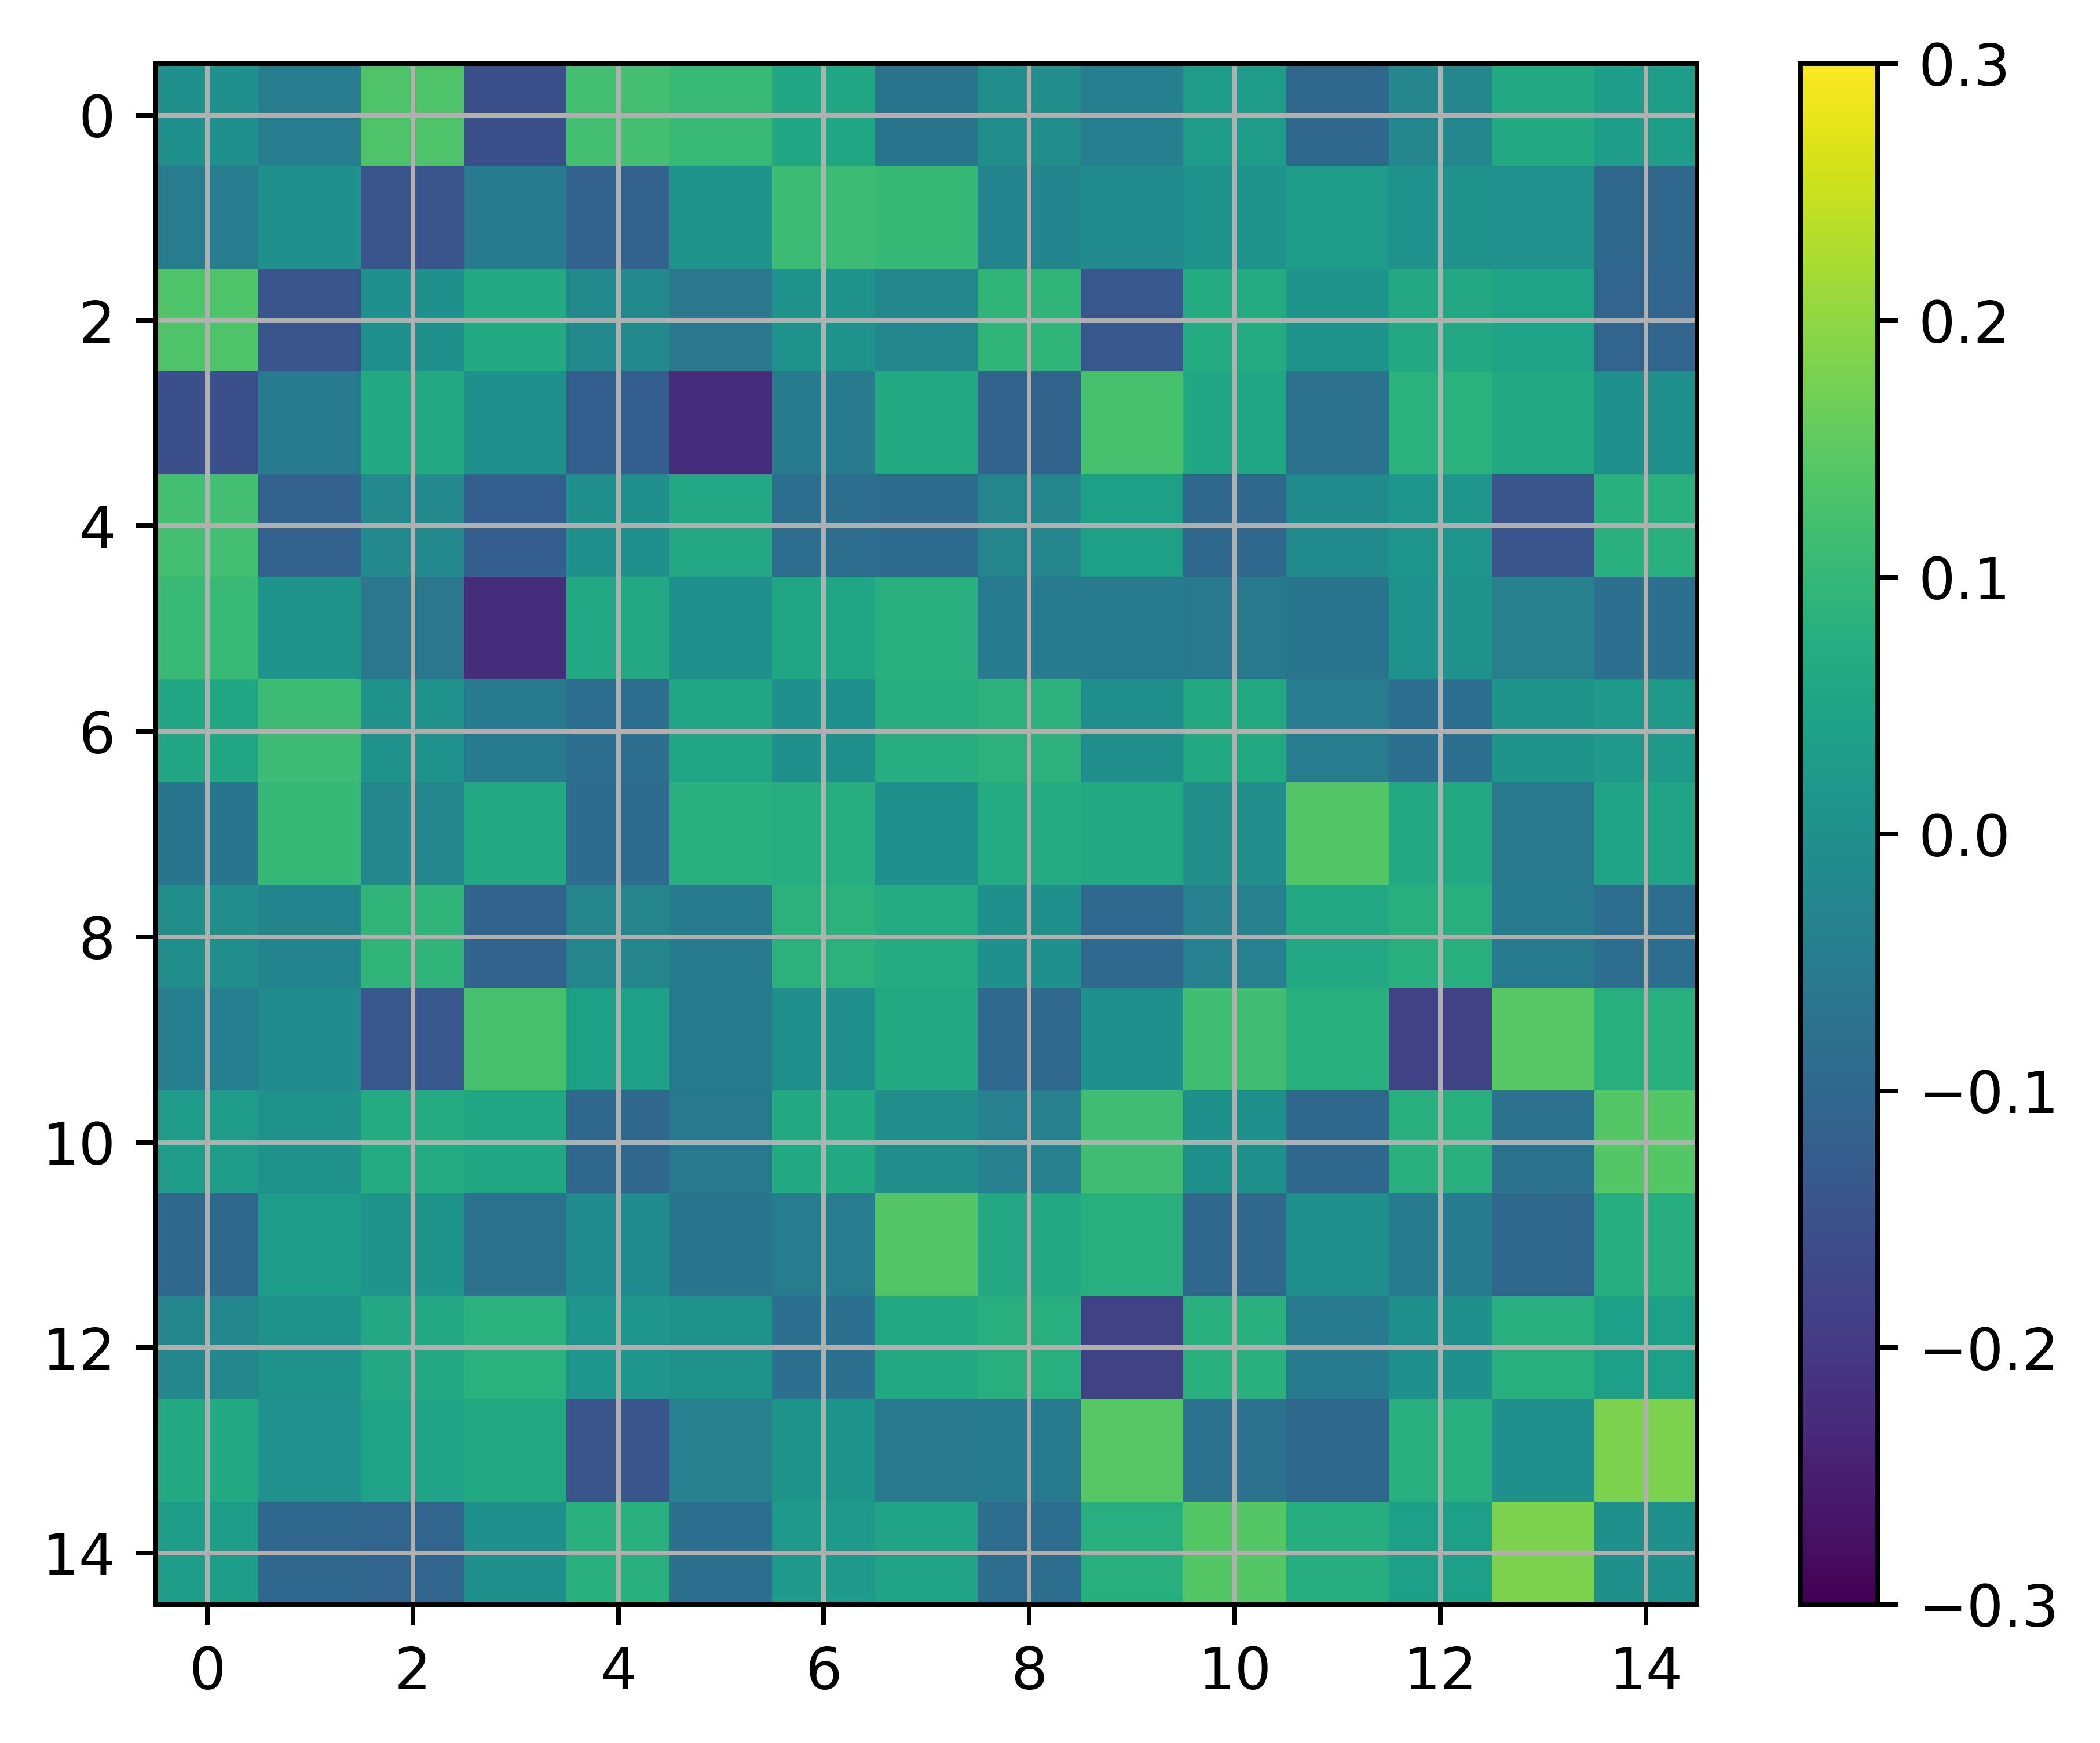
\includegraphics[width=0.2\textwidth]{../Analysis/DFC/size=480_step=180_rho=0.1/node=15_id=100206/c_20.jpg}
        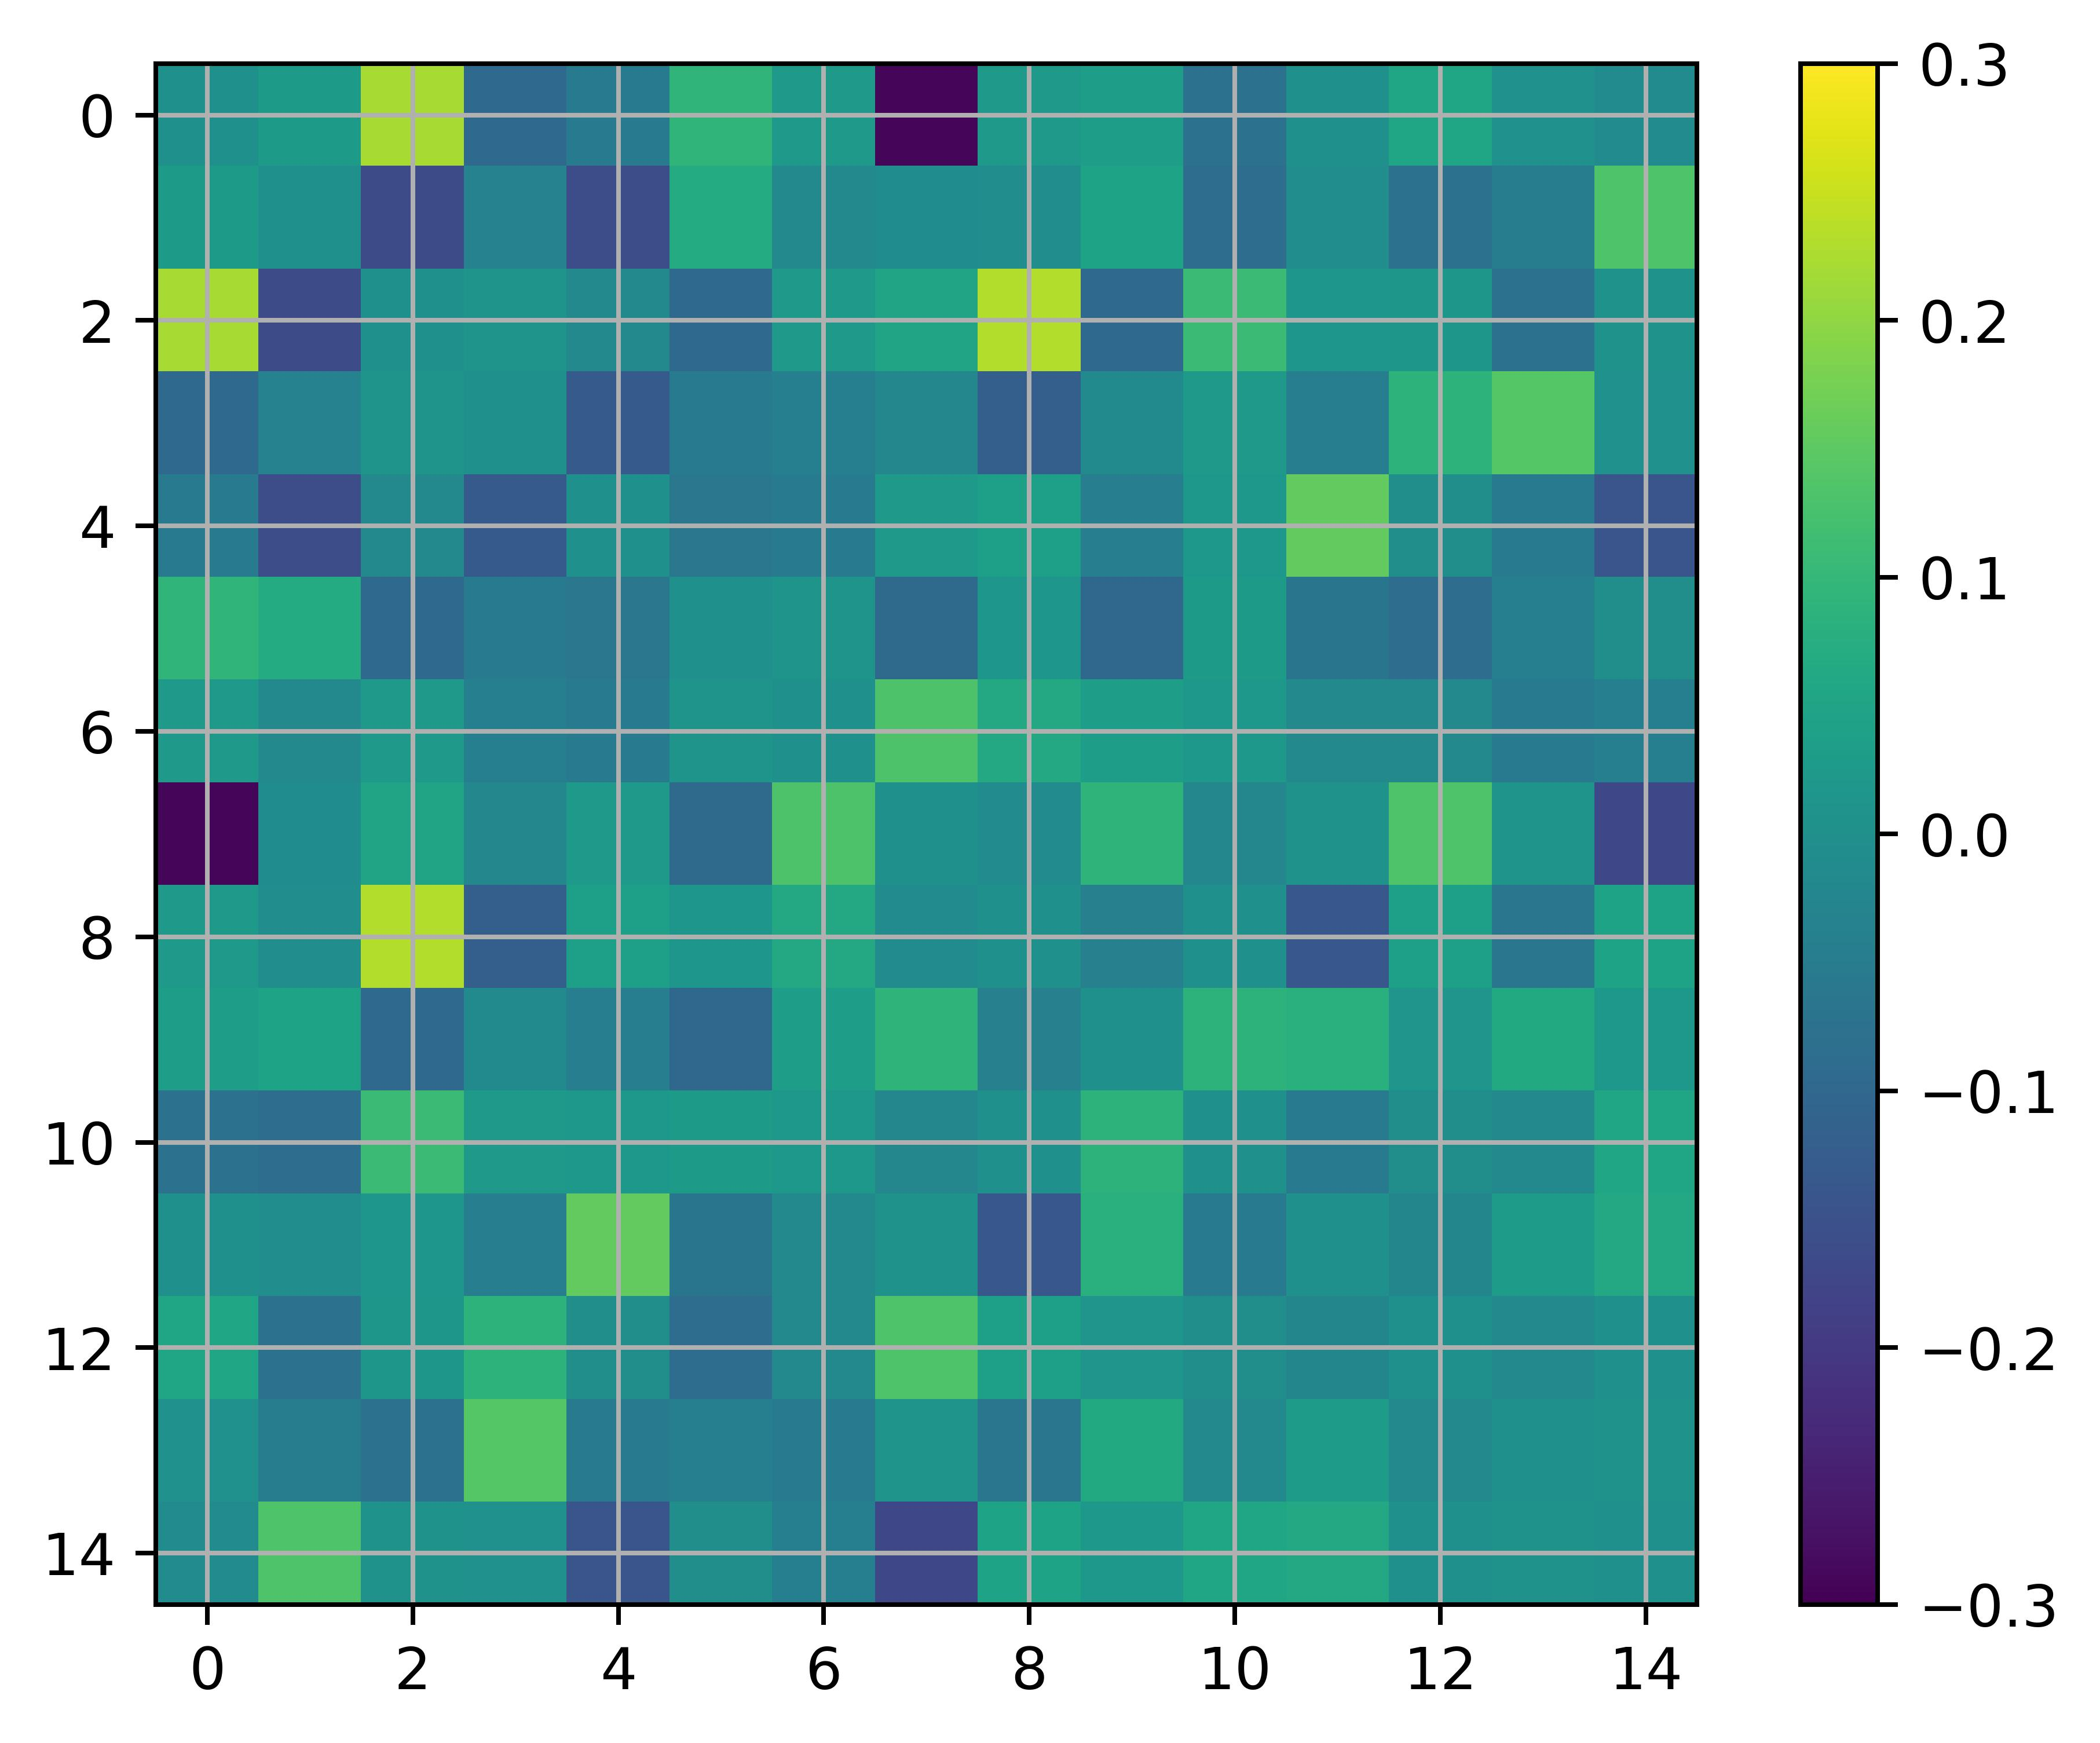
\includegraphics[width=0.2\textwidth]{../Analysis/DFC/size=480_step=180_rho=0.1/node=15_id=100206/c_22.jpg} \\
        \caption{Centered dynamic functional connectivity with $N_{node} = 15$.}
        % \label{LDA-example-1}
    \end{figure}

\end{frame}

\begin{frame}{Preprocessing - Examples}

    \begin{figure}[H]
        \centering
        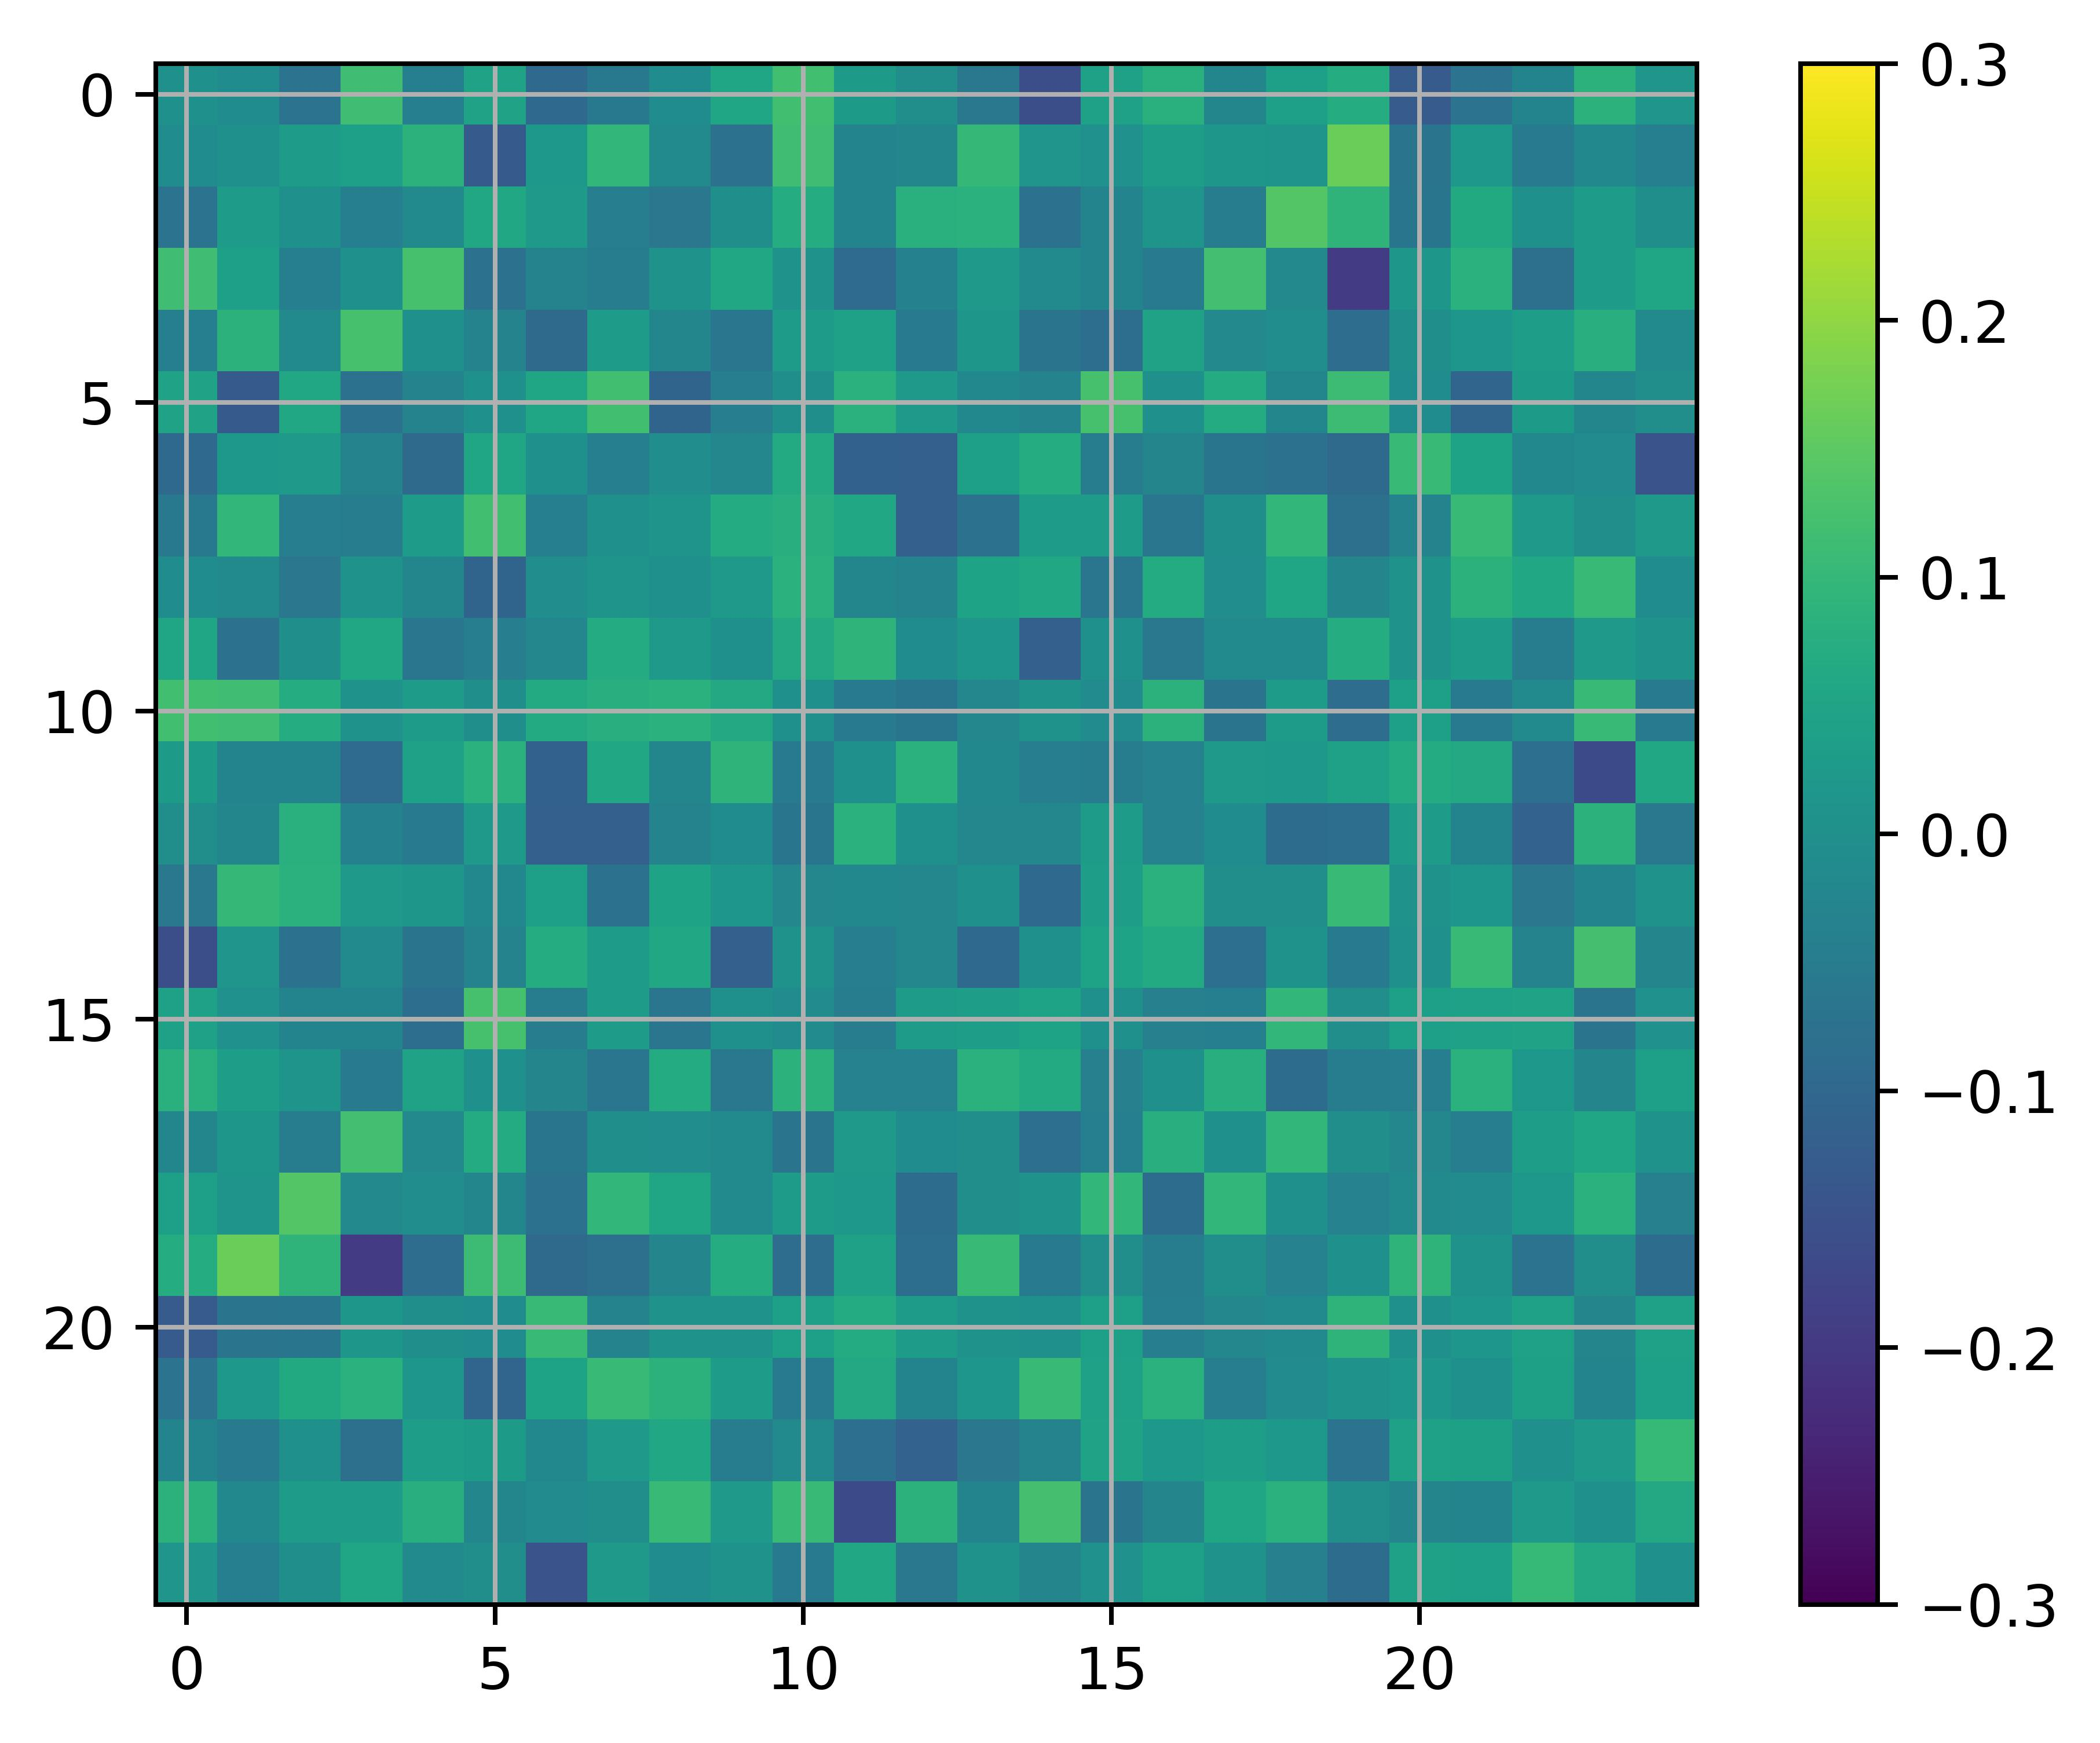
\includegraphics[width=0.2\textwidth]{../Analysis/DFC/size=480_step=180_rho=0.1/node=25_id=100206/c_0.jpg}
        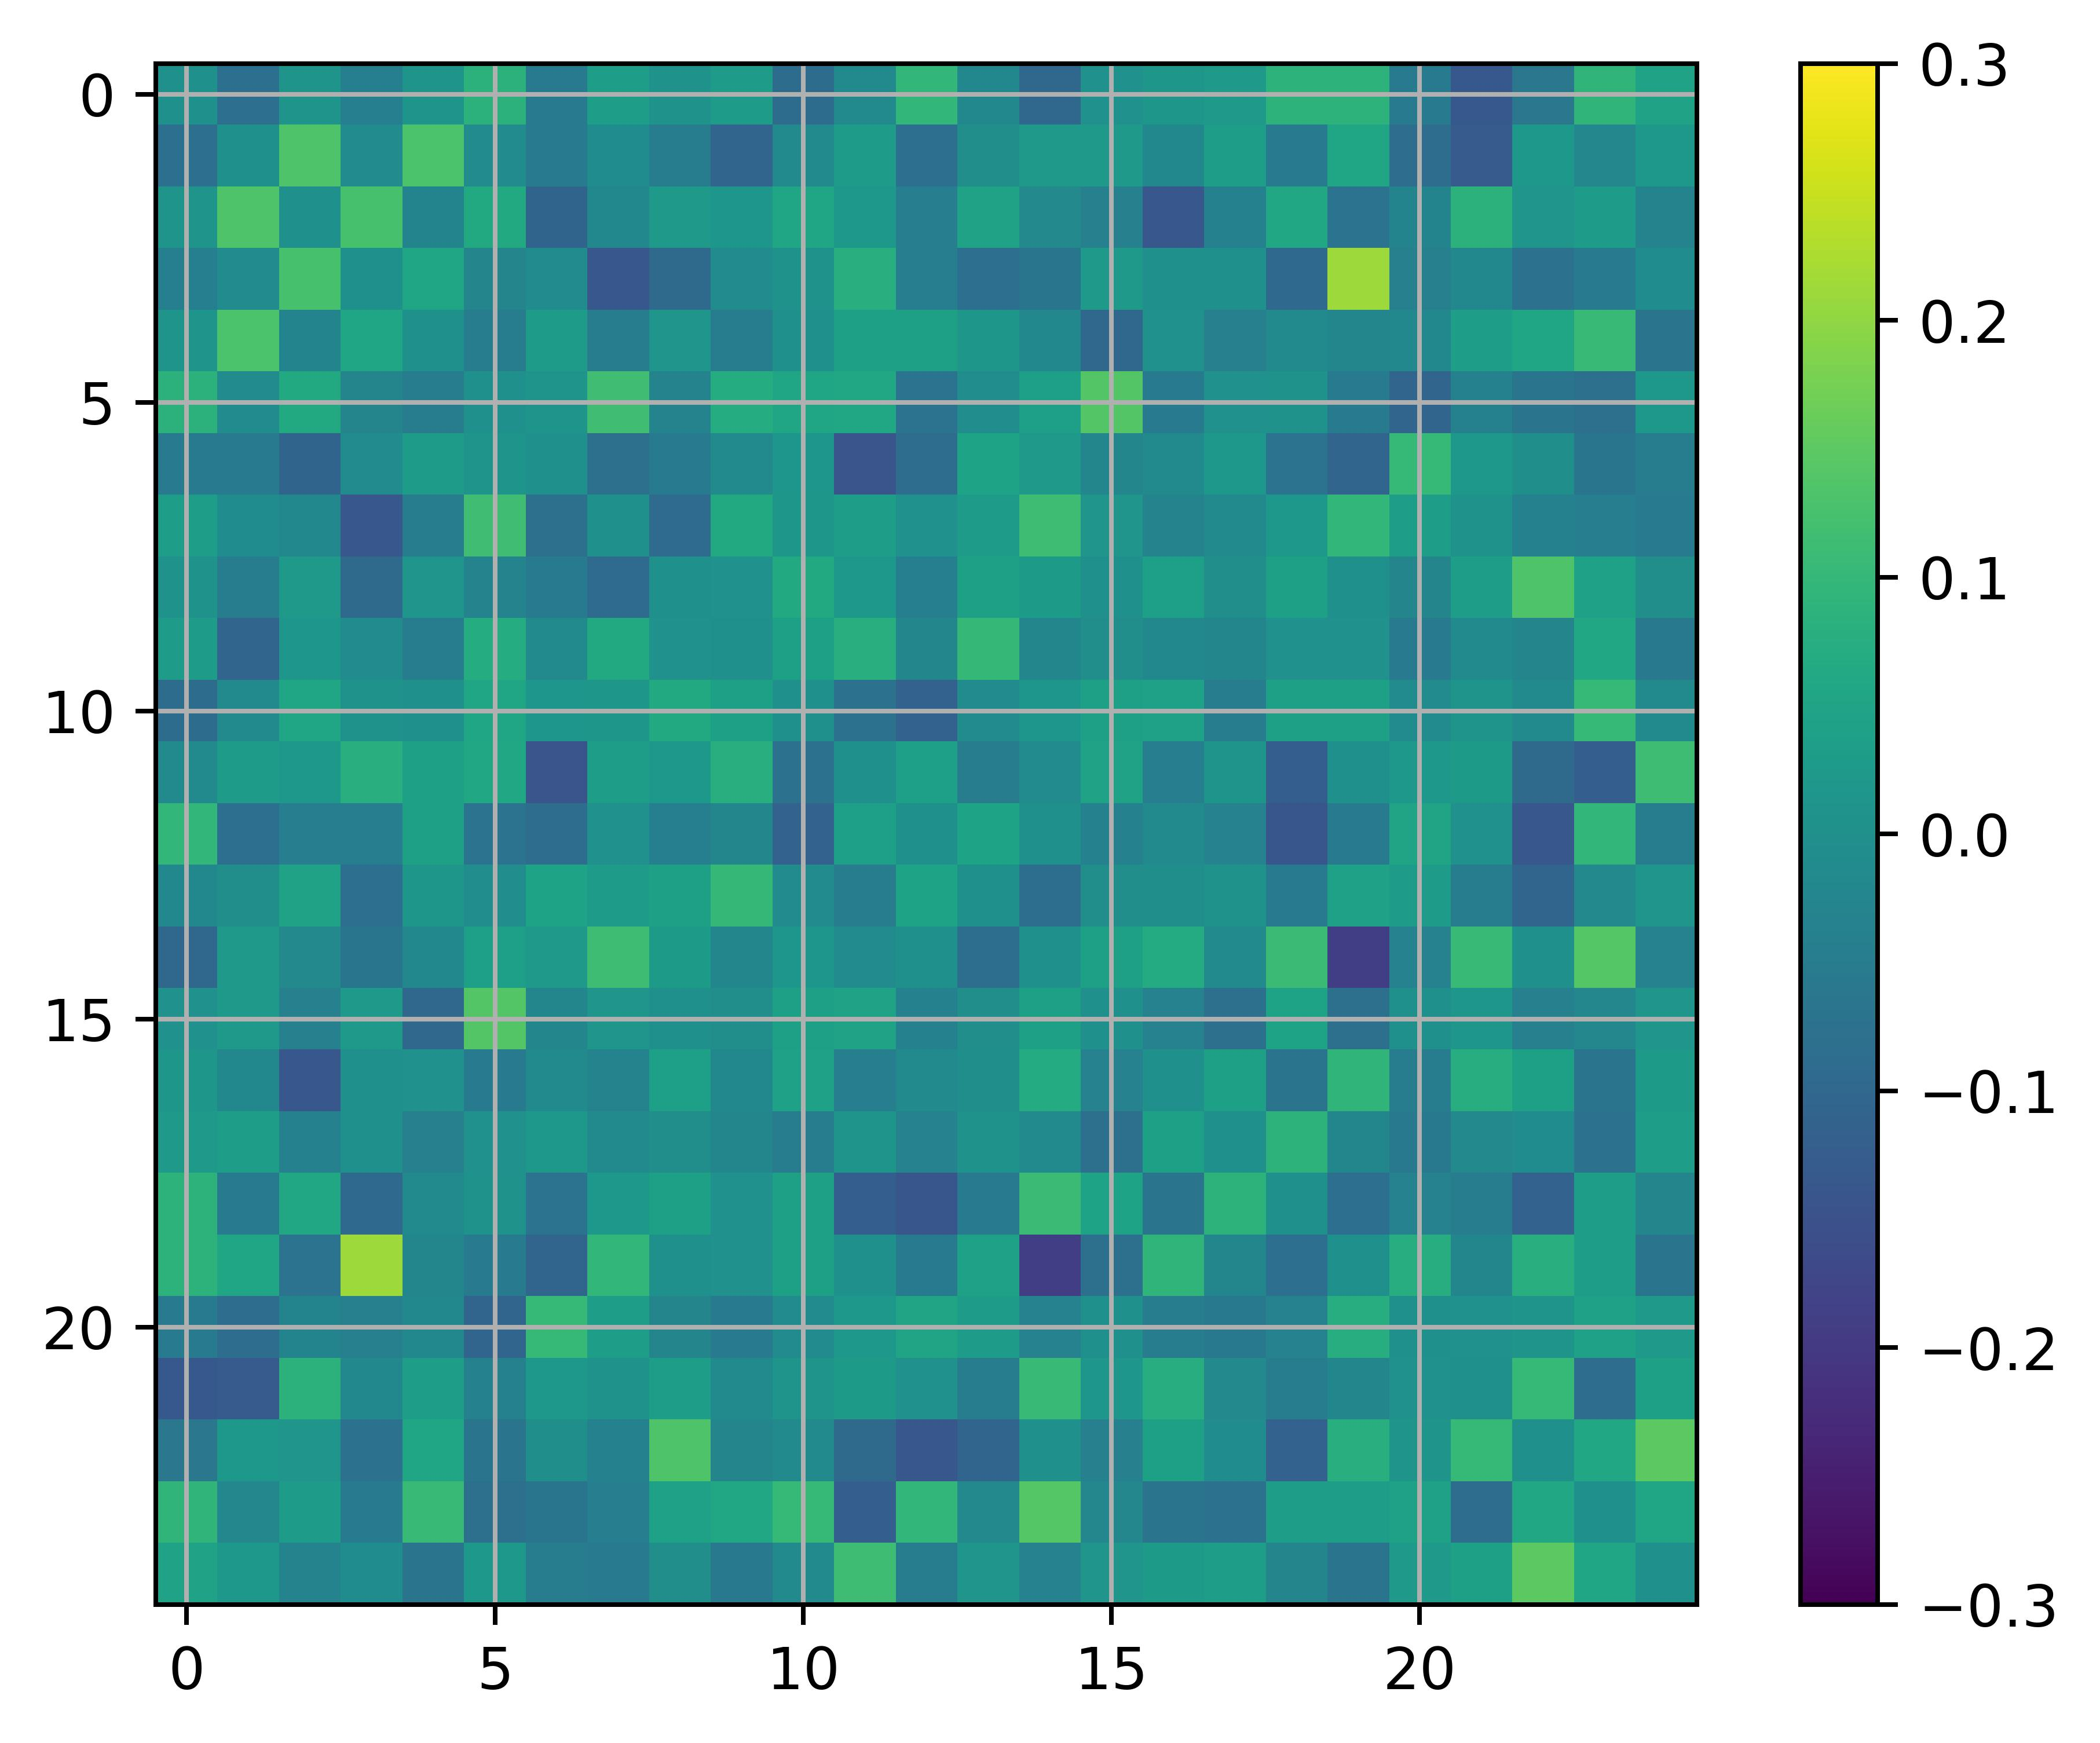
\includegraphics[width=0.2\textwidth]{../Analysis/DFC/size=480_step=180_rho=0.1/node=25_id=100206/c_2.jpg}
        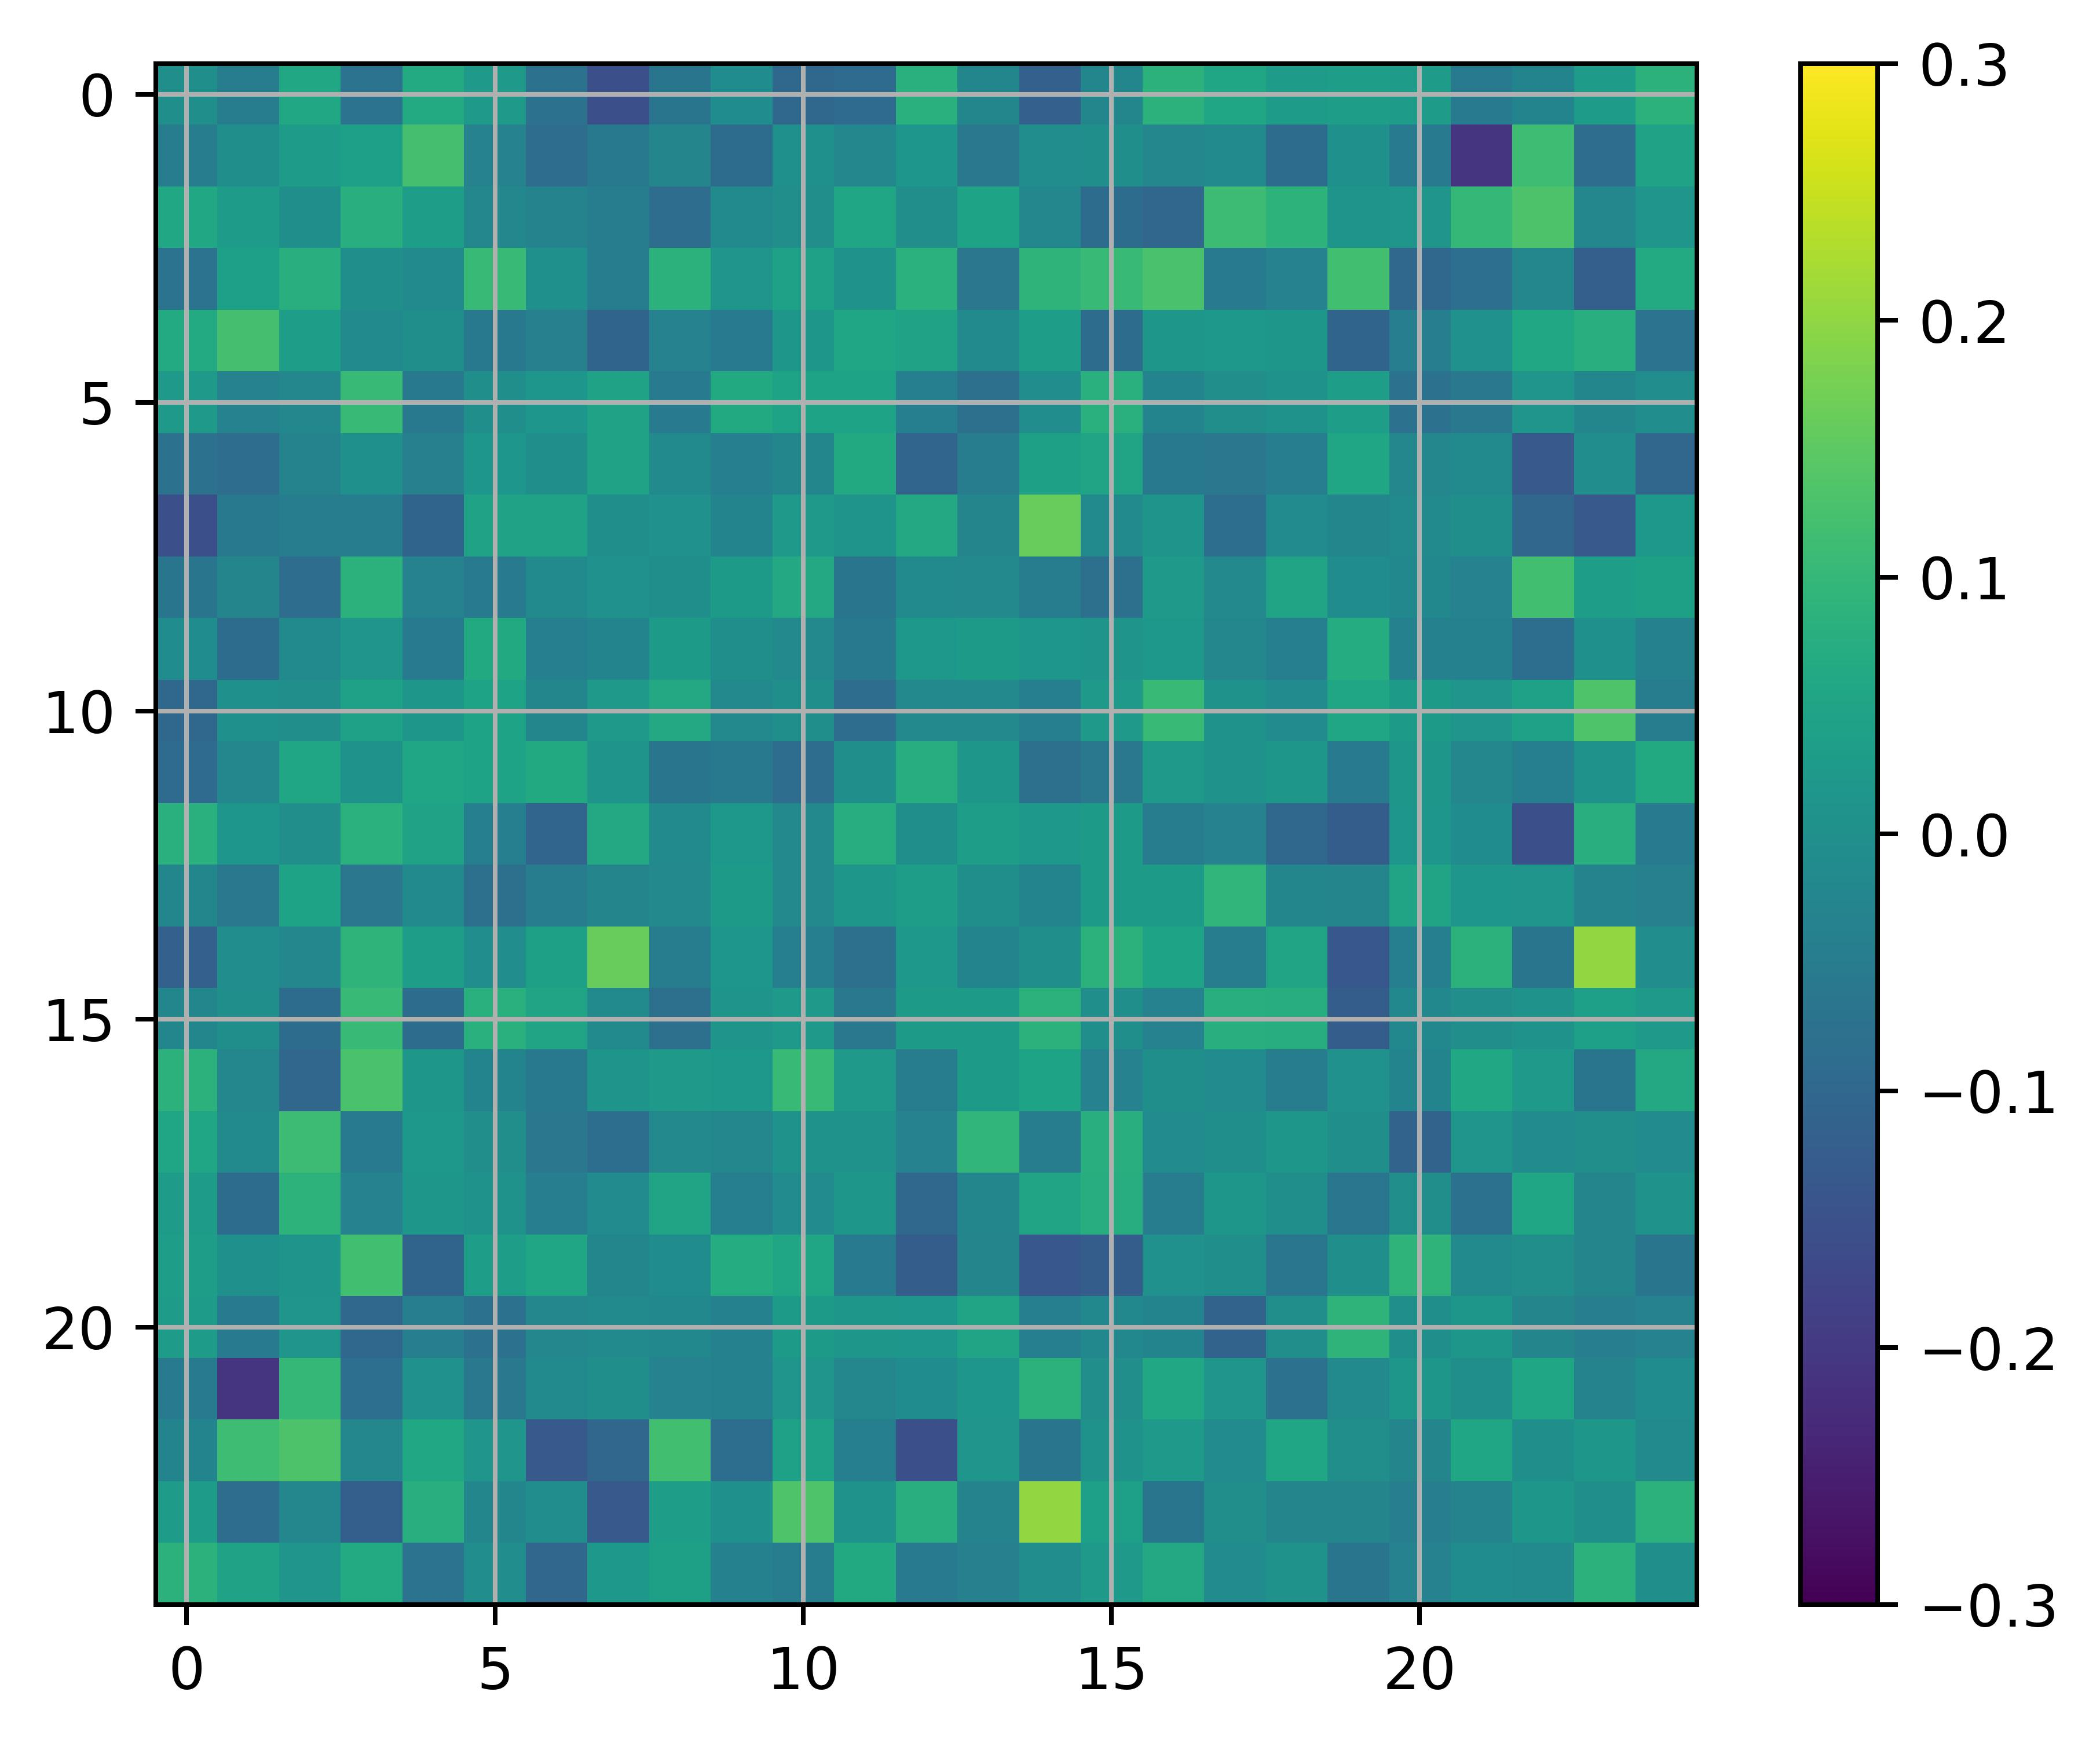
\includegraphics[width=0.2\textwidth]{../Analysis/DFC/size=480_step=180_rho=0.1/node=25_id=100206/c_4.jpg}
        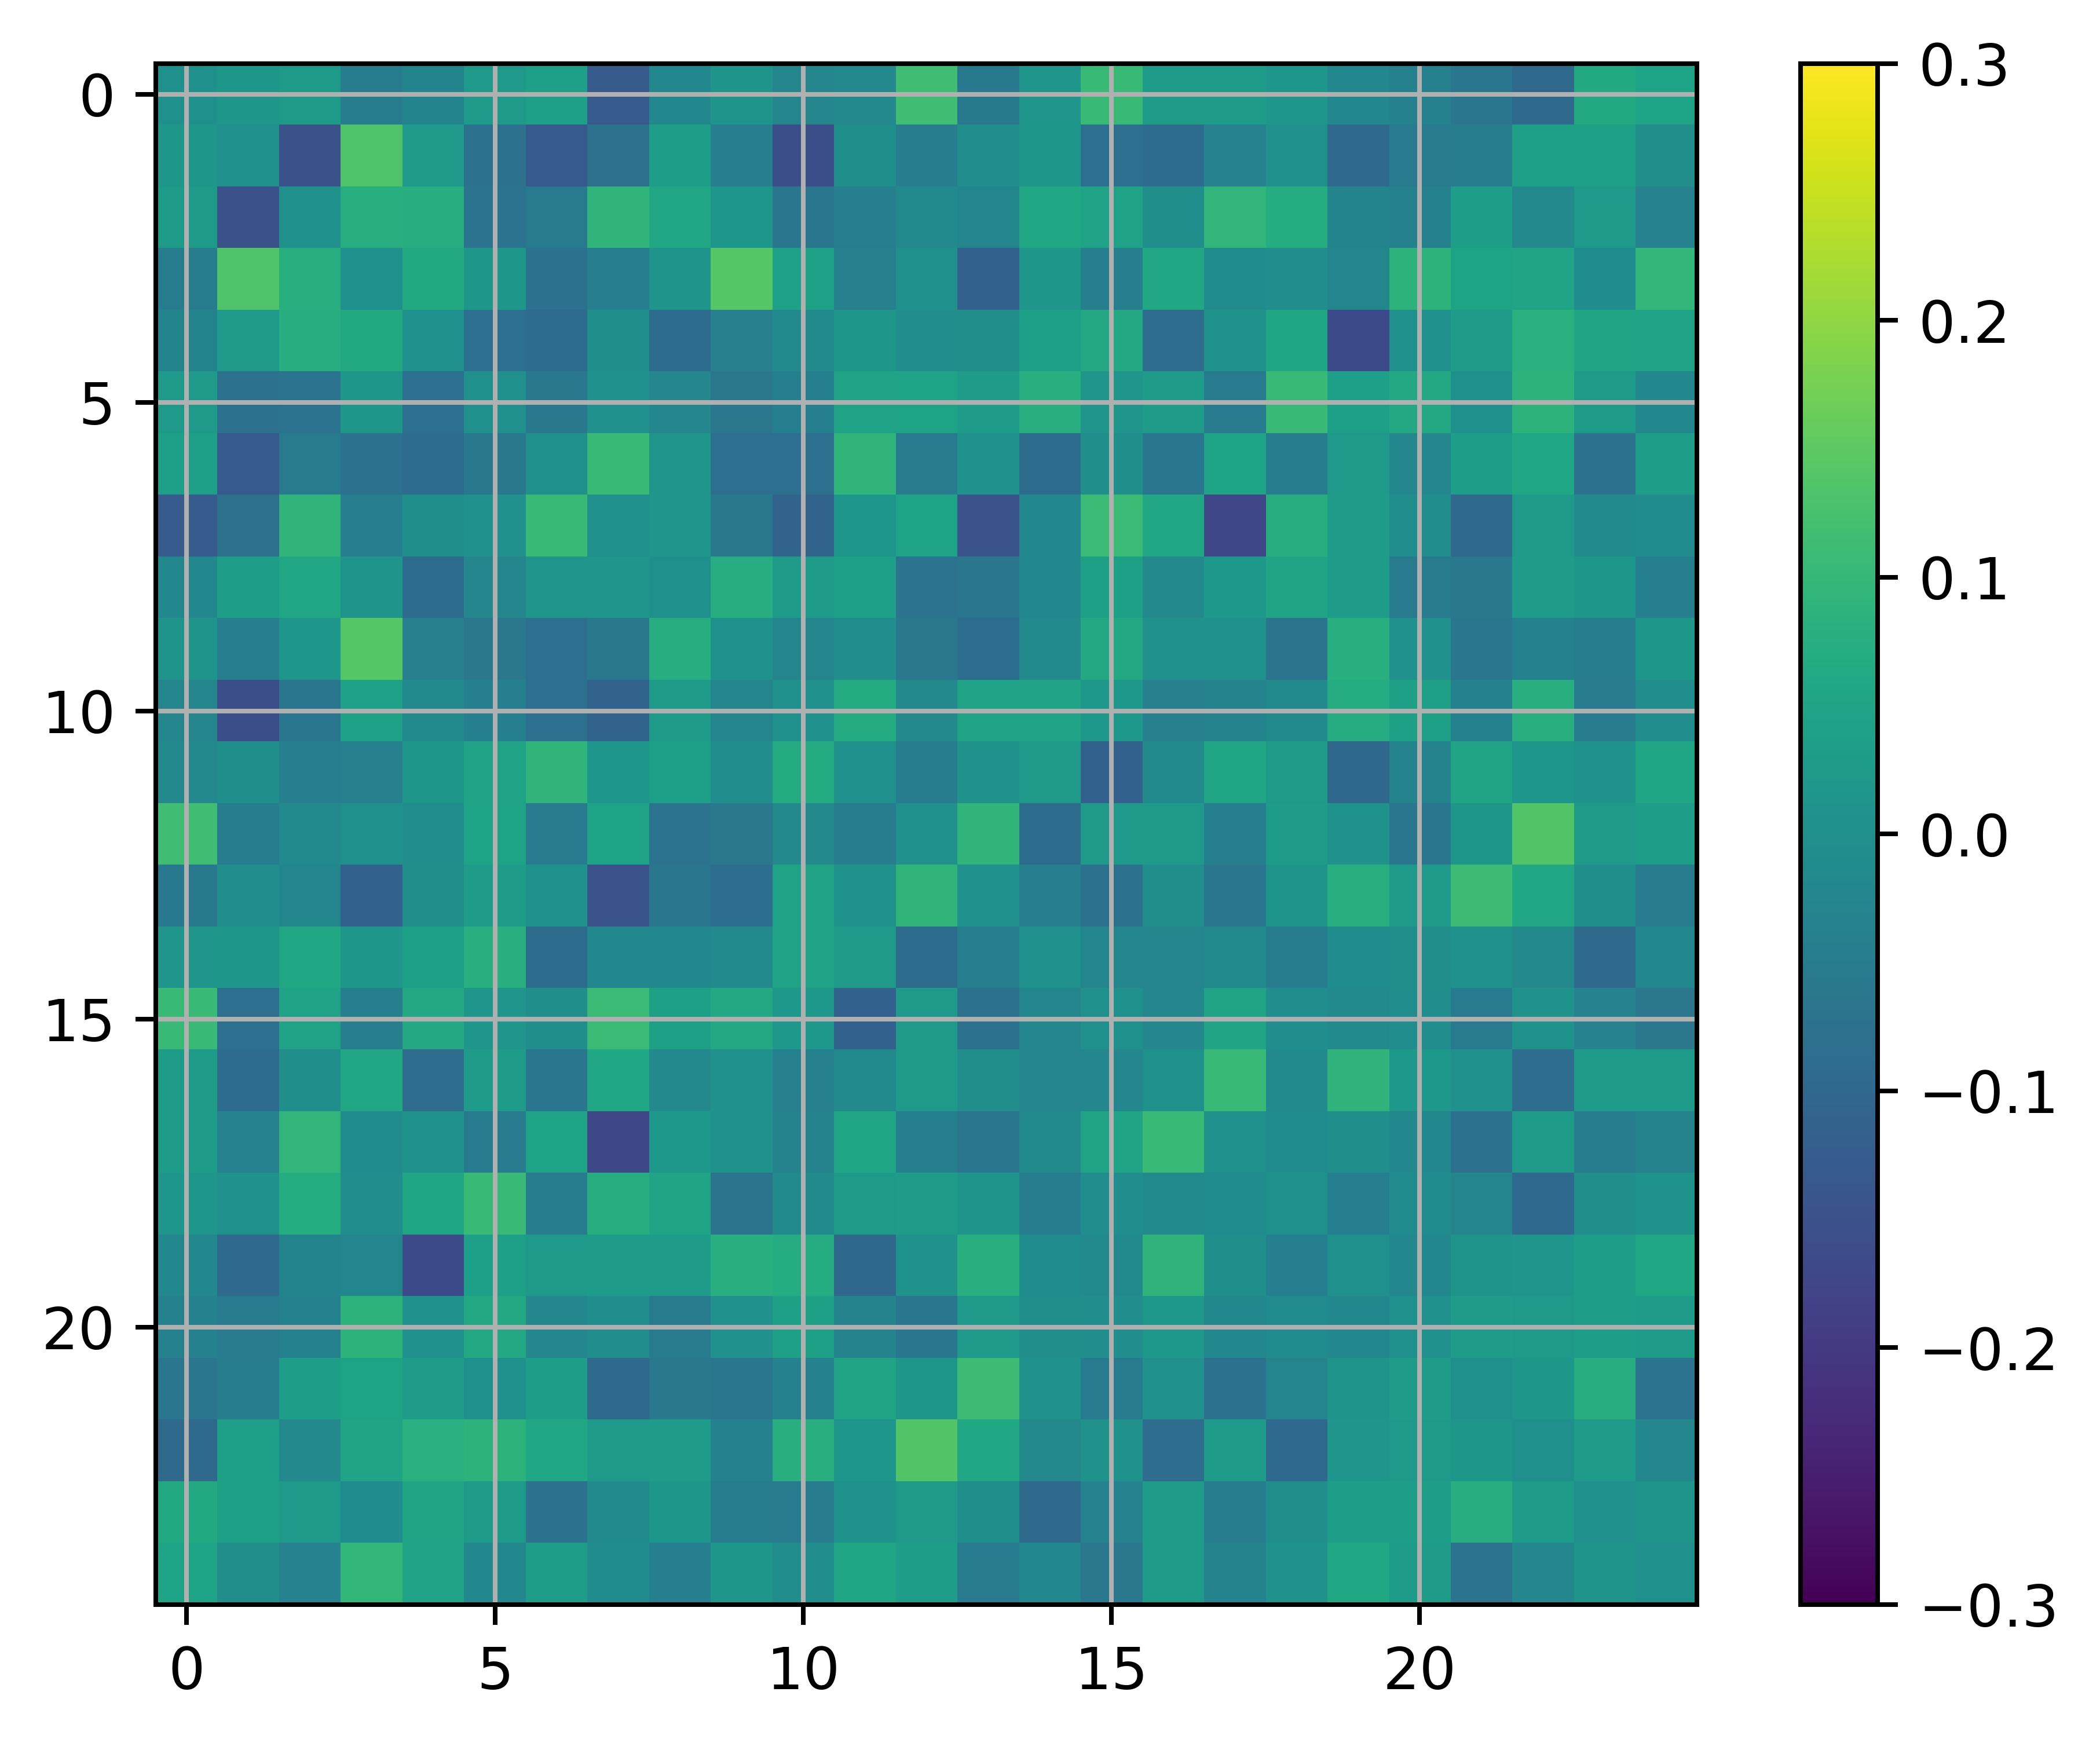
\includegraphics[width=0.2\textwidth]{../Analysis/DFC/size=480_step=180_rho=0.1/node=25_id=100206/c_6.jpg} \\
        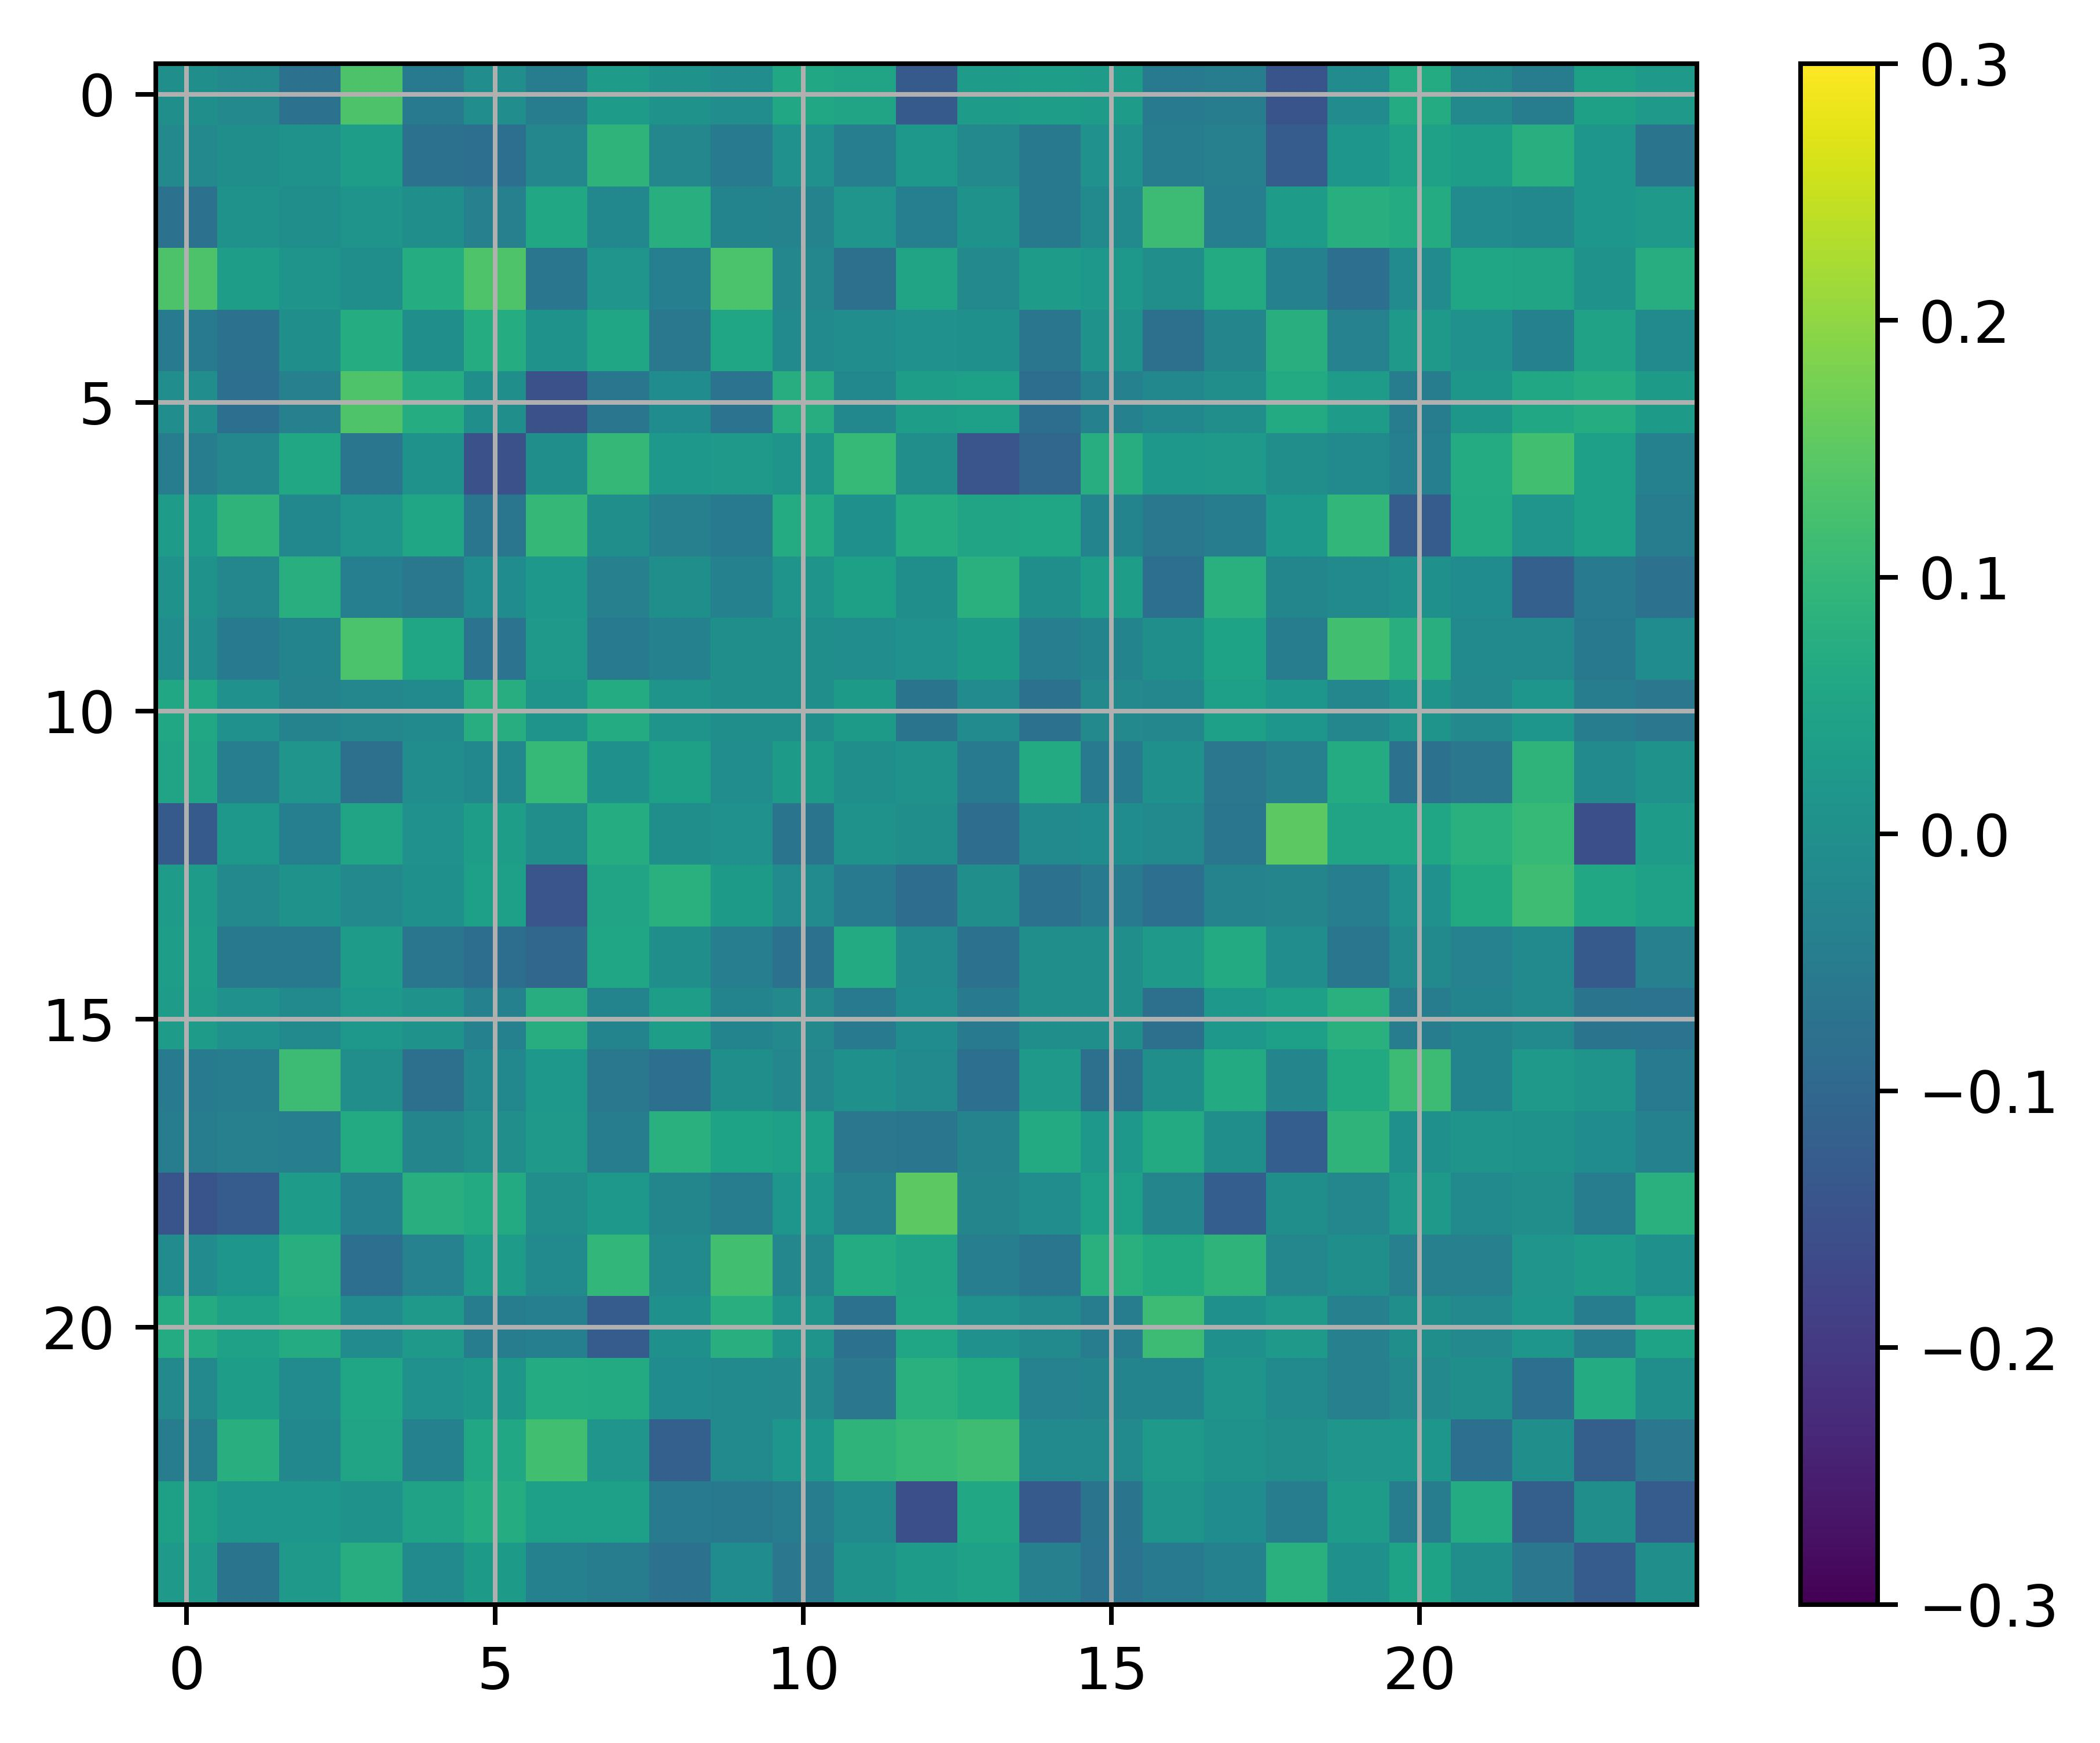
\includegraphics[width=0.2\textwidth]{../Analysis/DFC/size=480_step=180_rho=0.1/node=25_id=100206/c_8.jpg}
        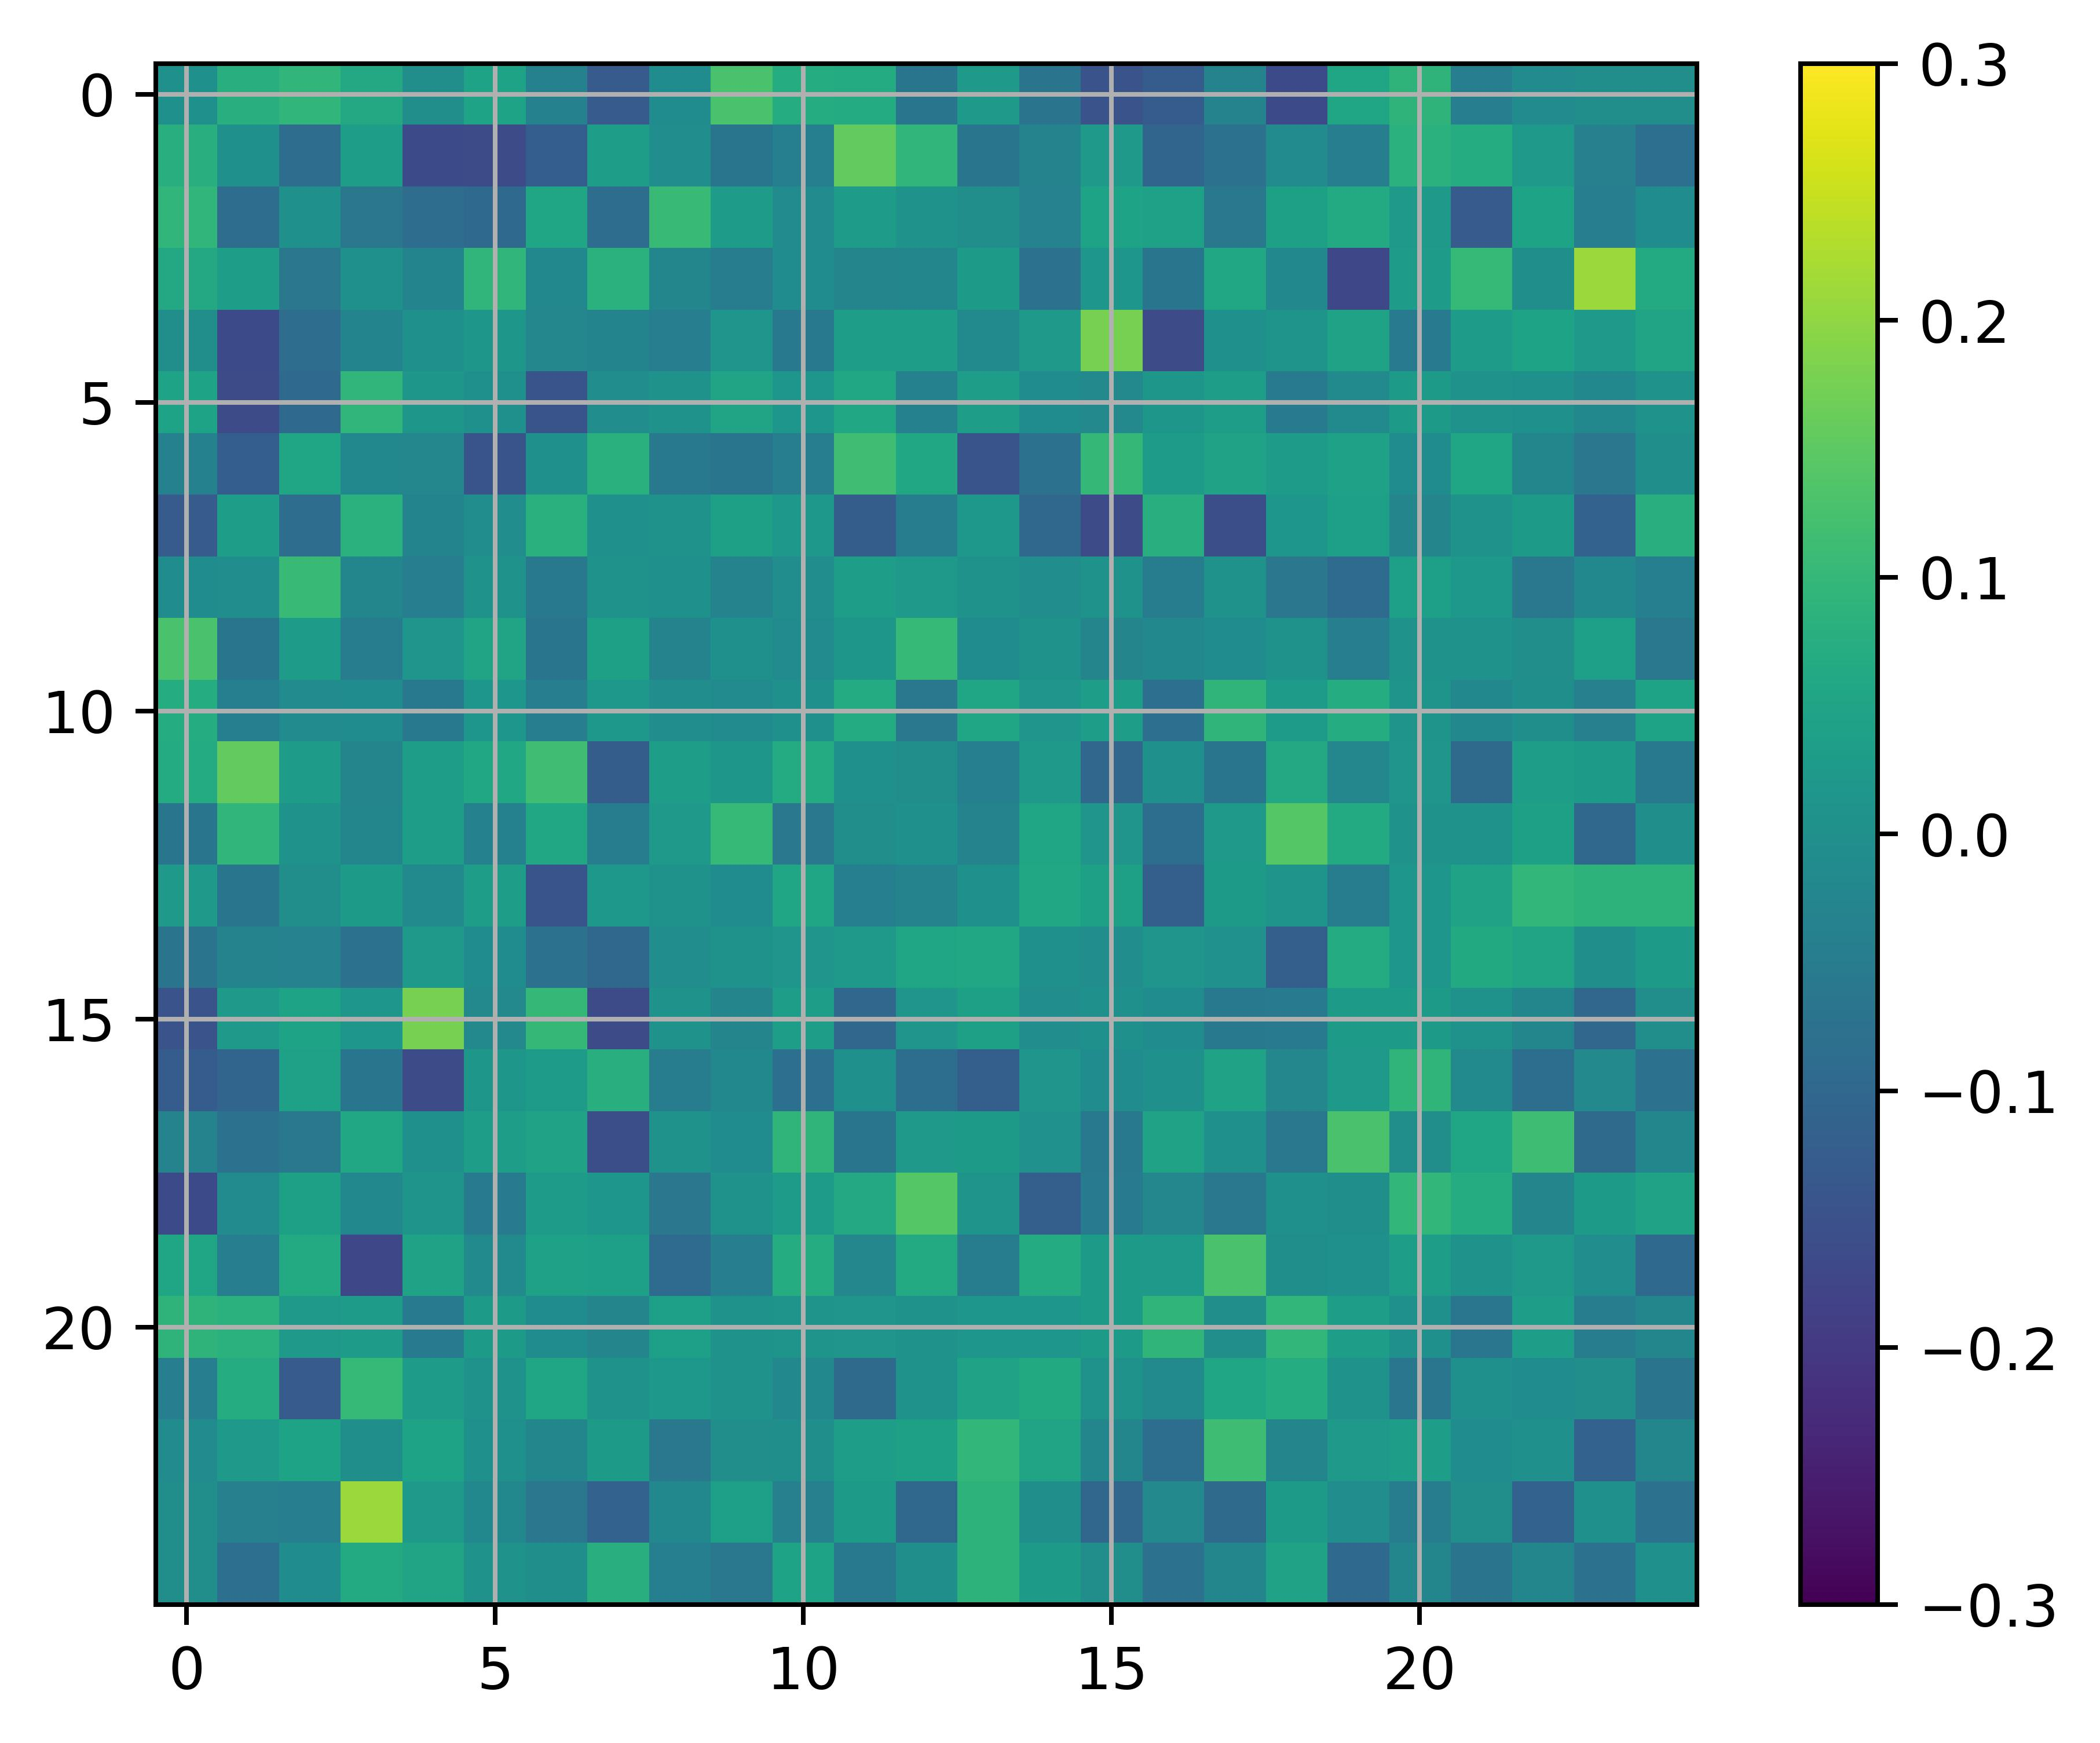
\includegraphics[width=0.2\textwidth]{../Analysis/DFC/size=480_step=180_rho=0.1/node=25_id=100206/c_10.jpg}
        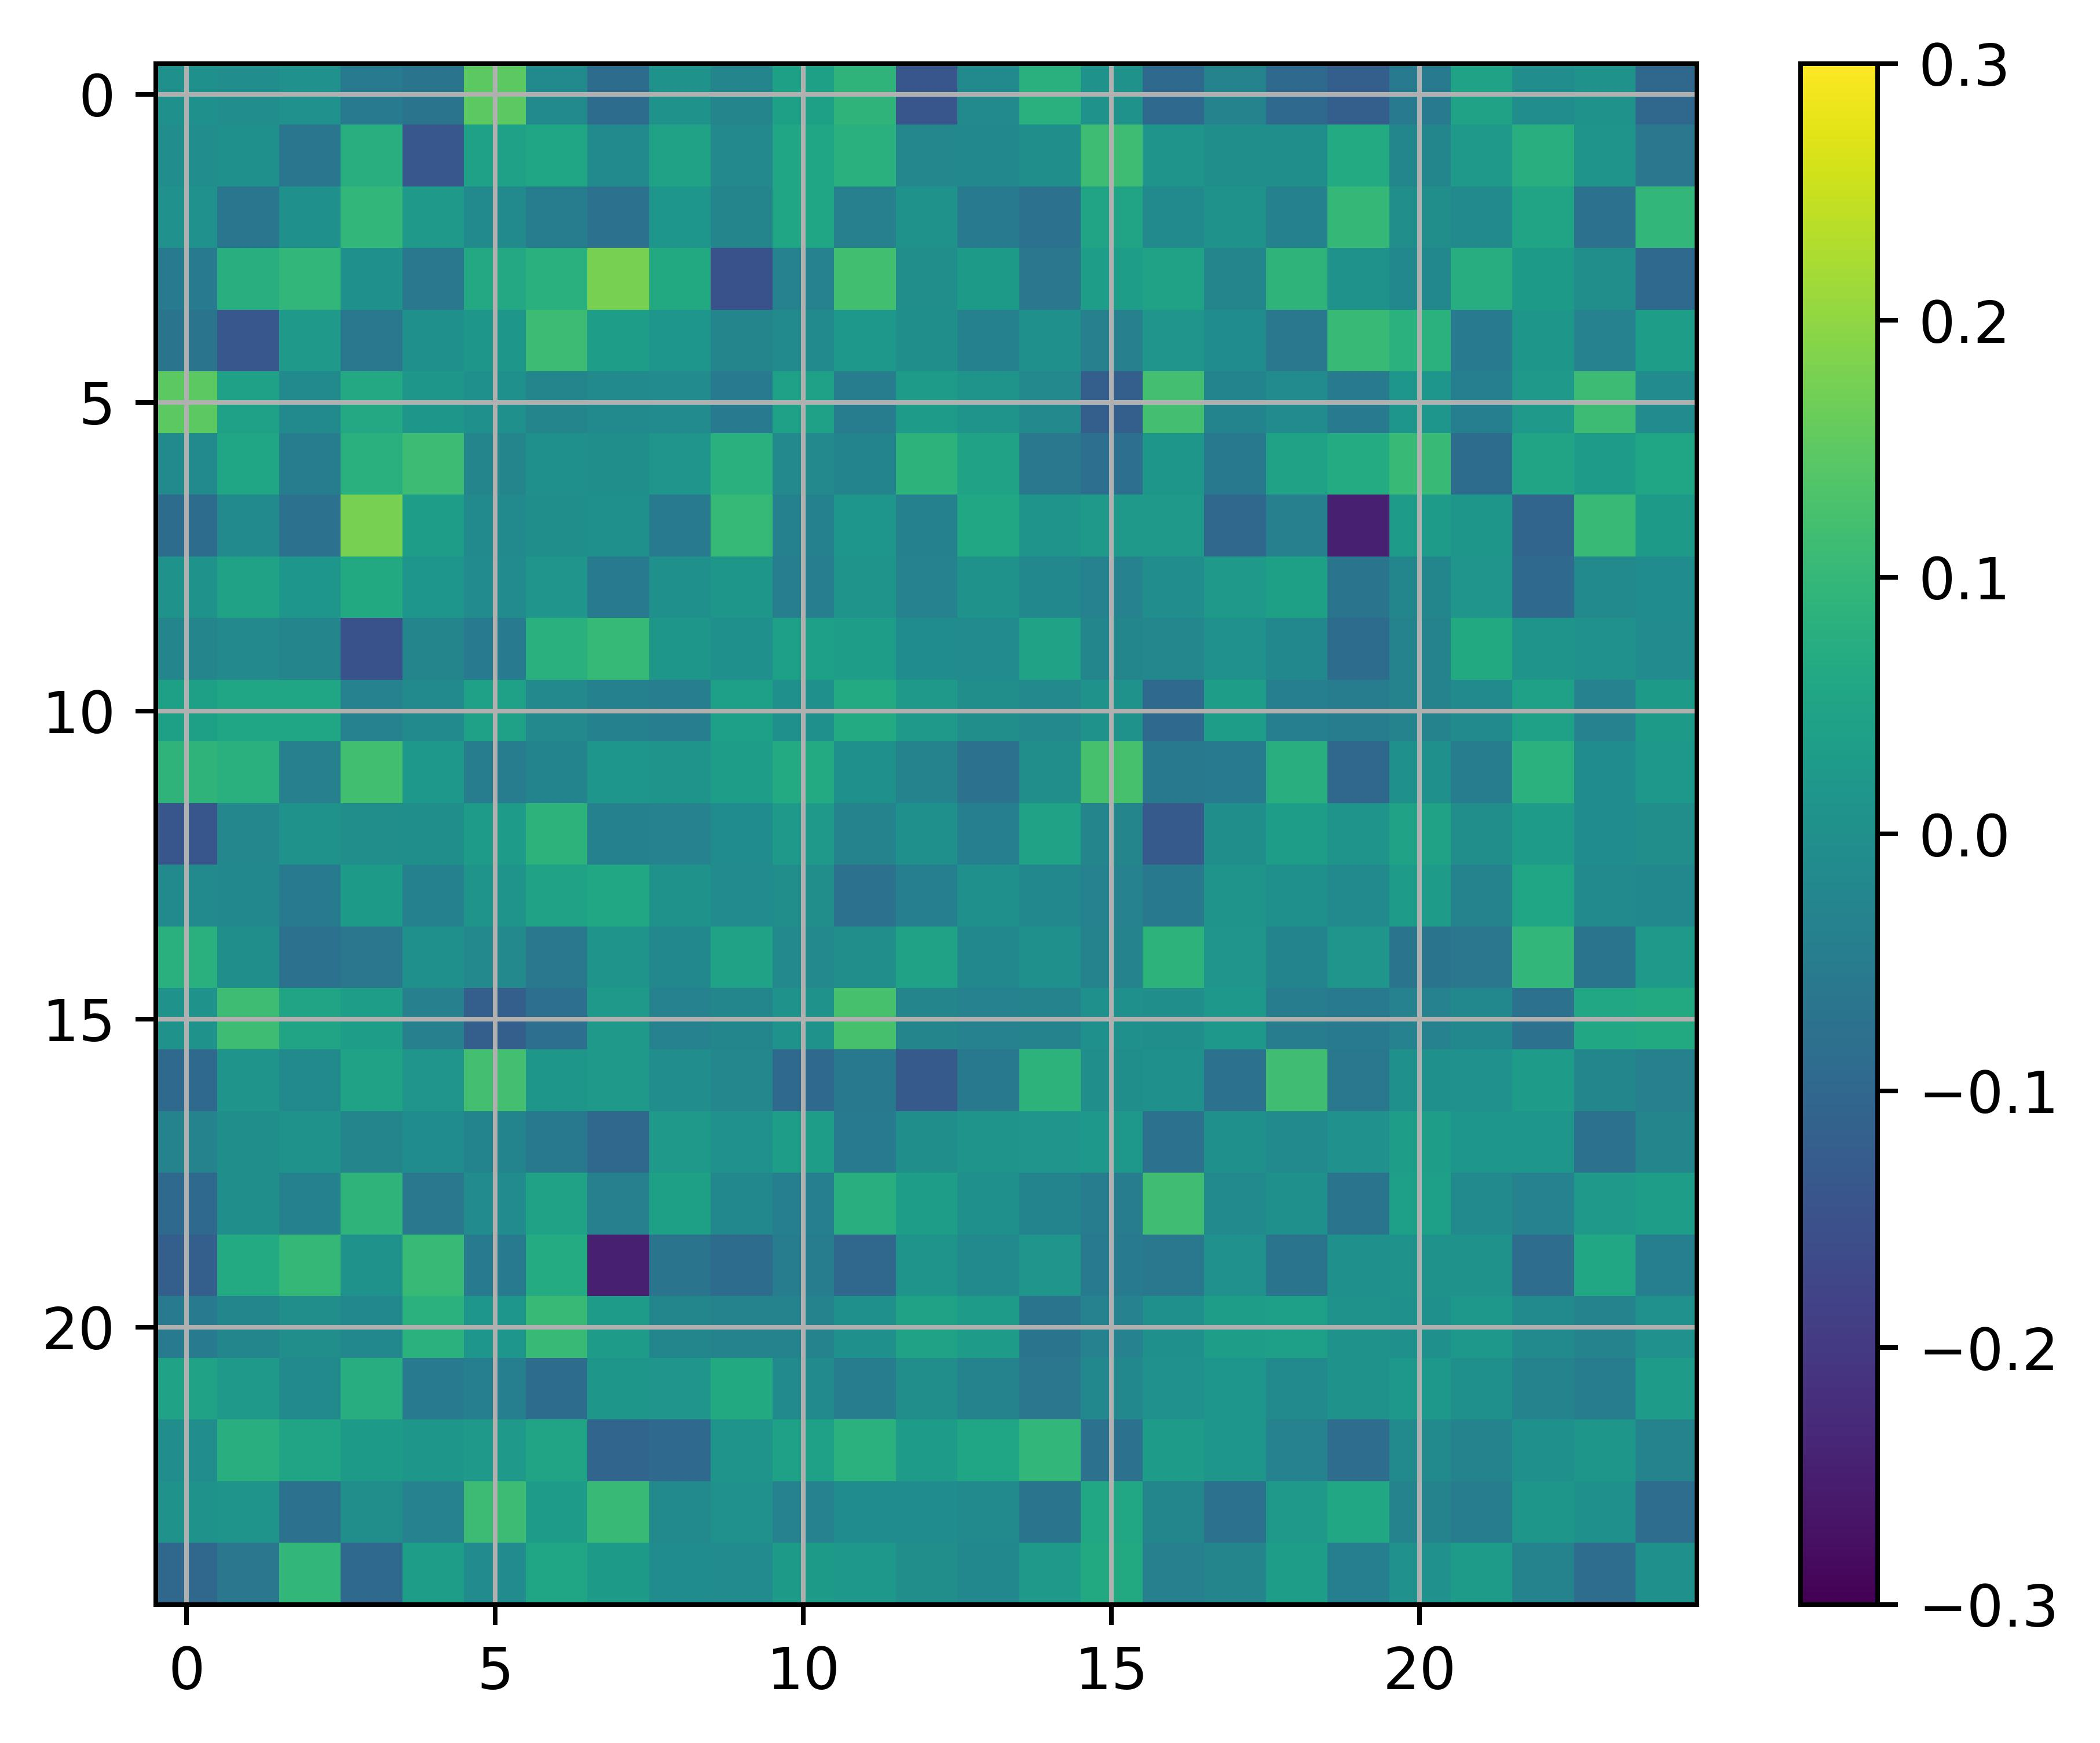
\includegraphics[width=0.2\textwidth]{../Analysis/DFC/size=480_step=180_rho=0.1/node=25_id=100206/c_12.jpg}
        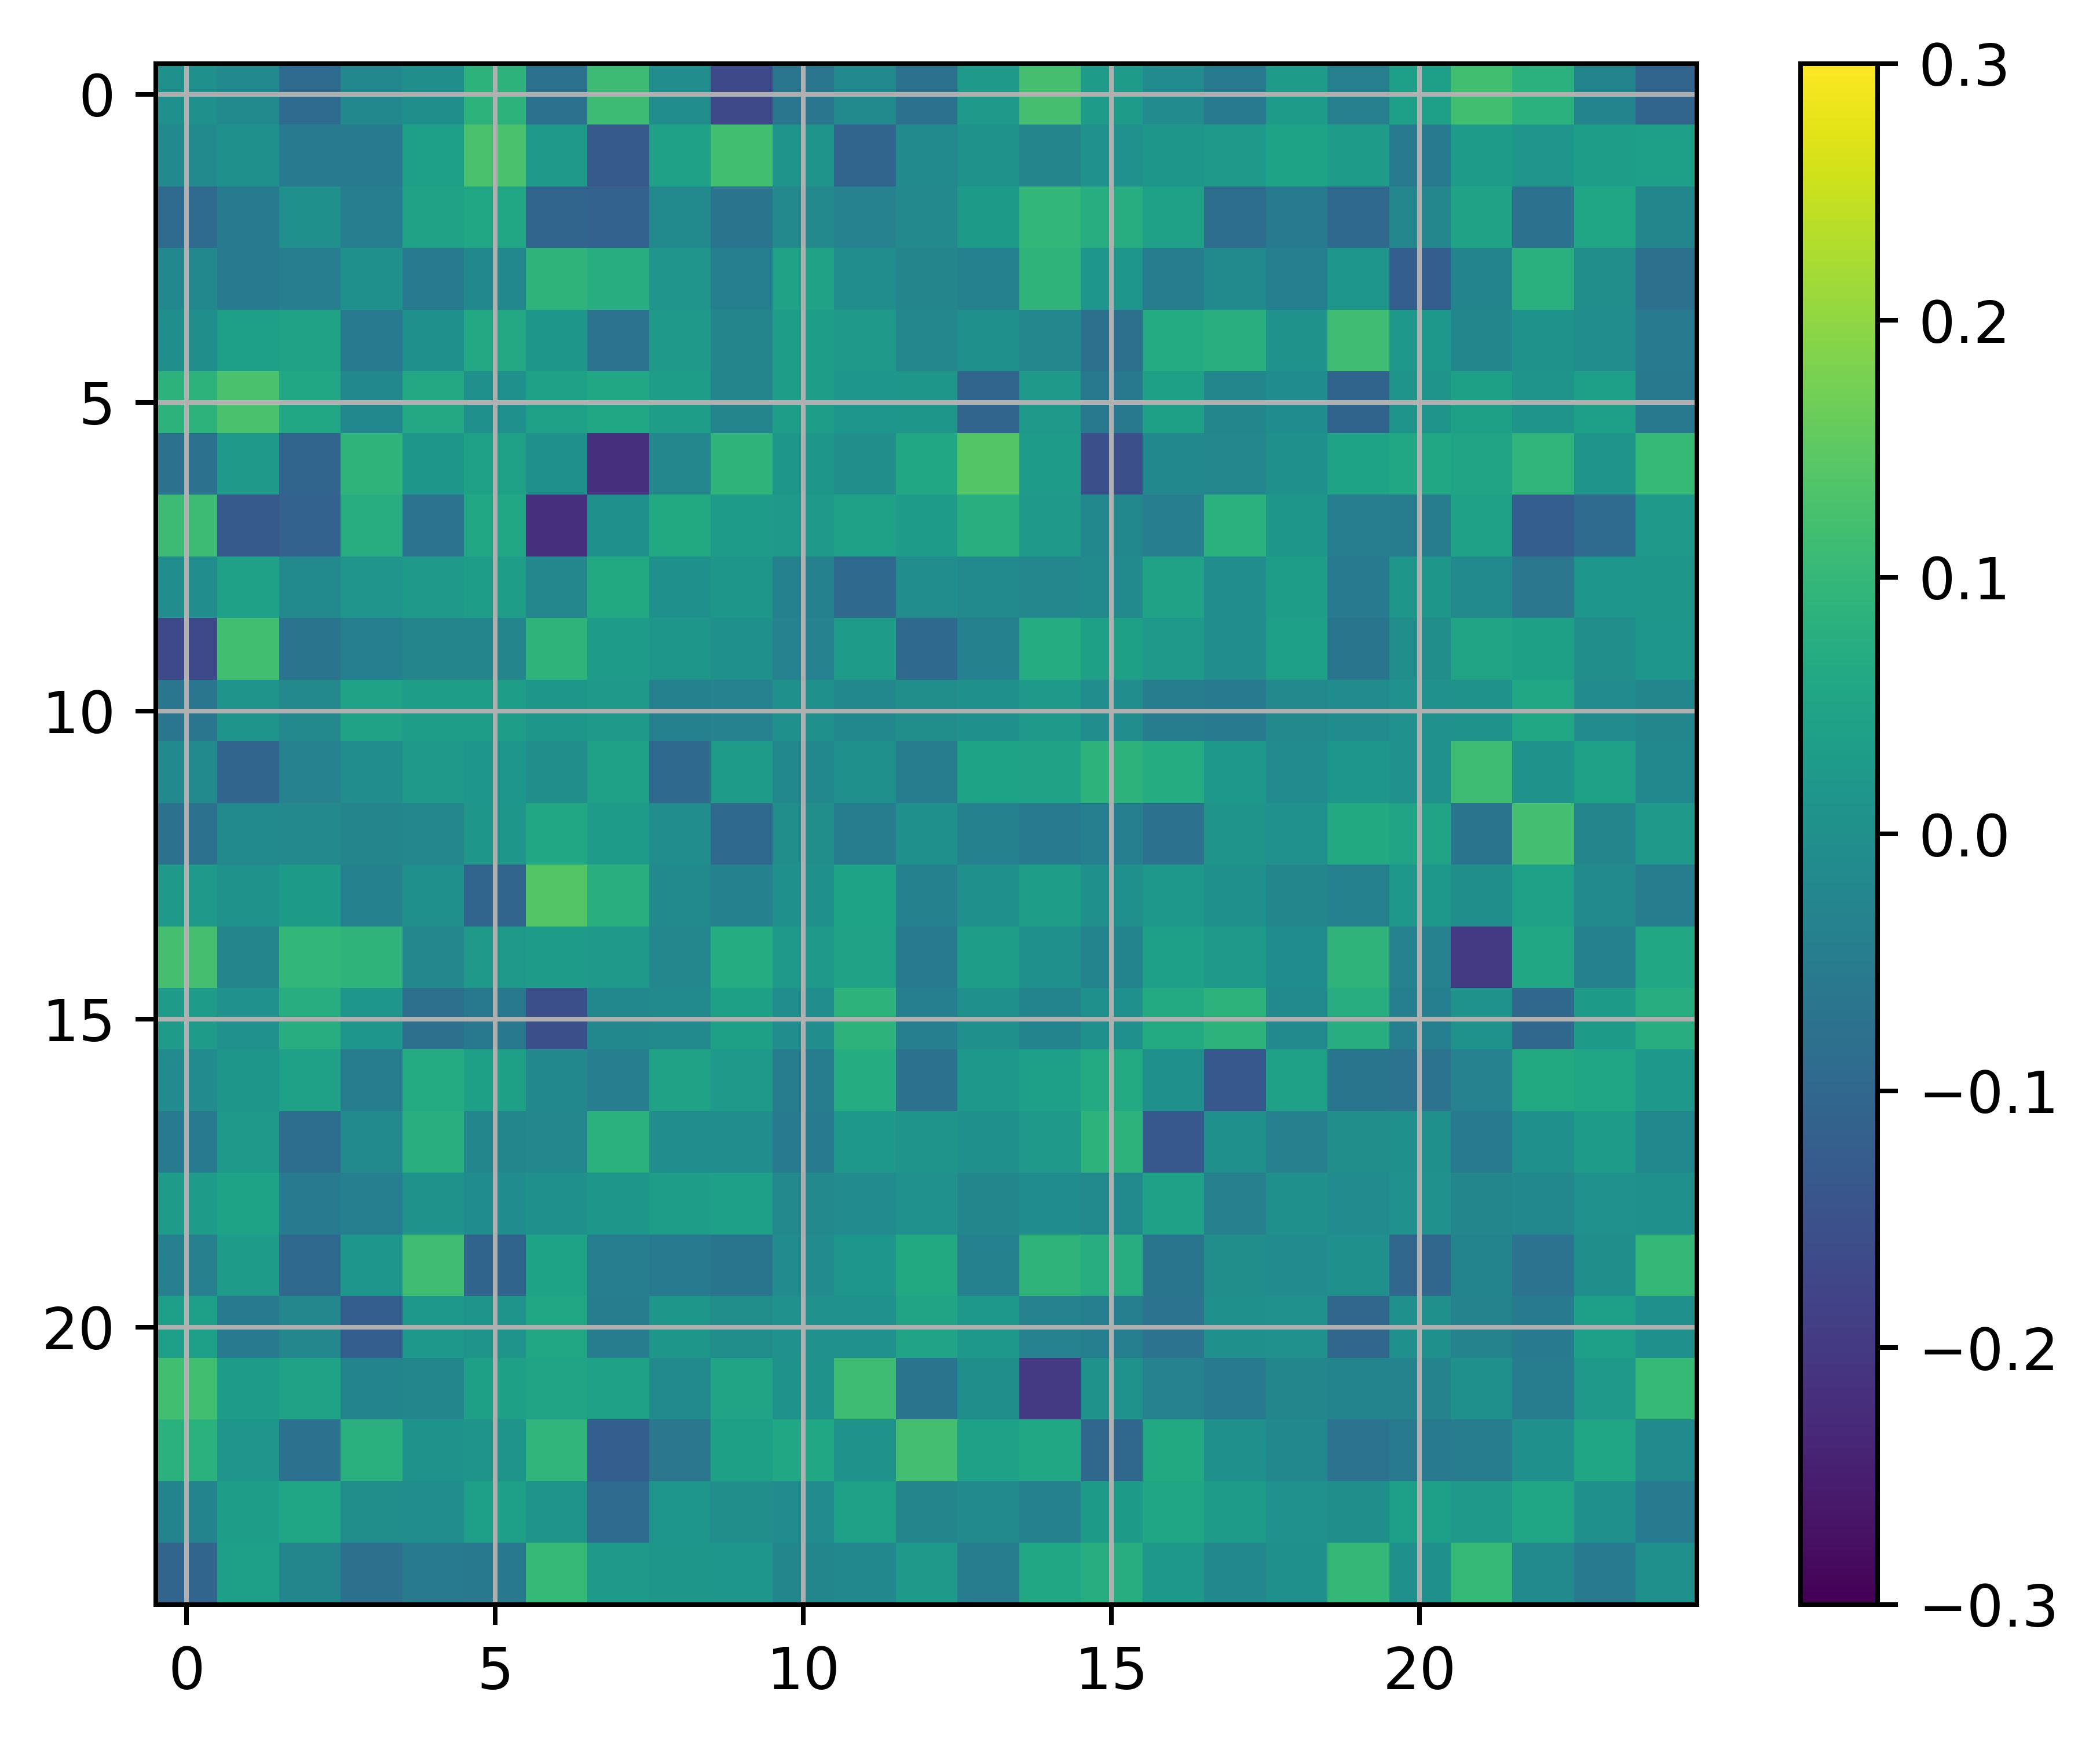
\includegraphics[width=0.2\textwidth]{../Analysis/DFC/size=480_step=180_rho=0.1/node=25_id=100206/c_14.jpg} \\
        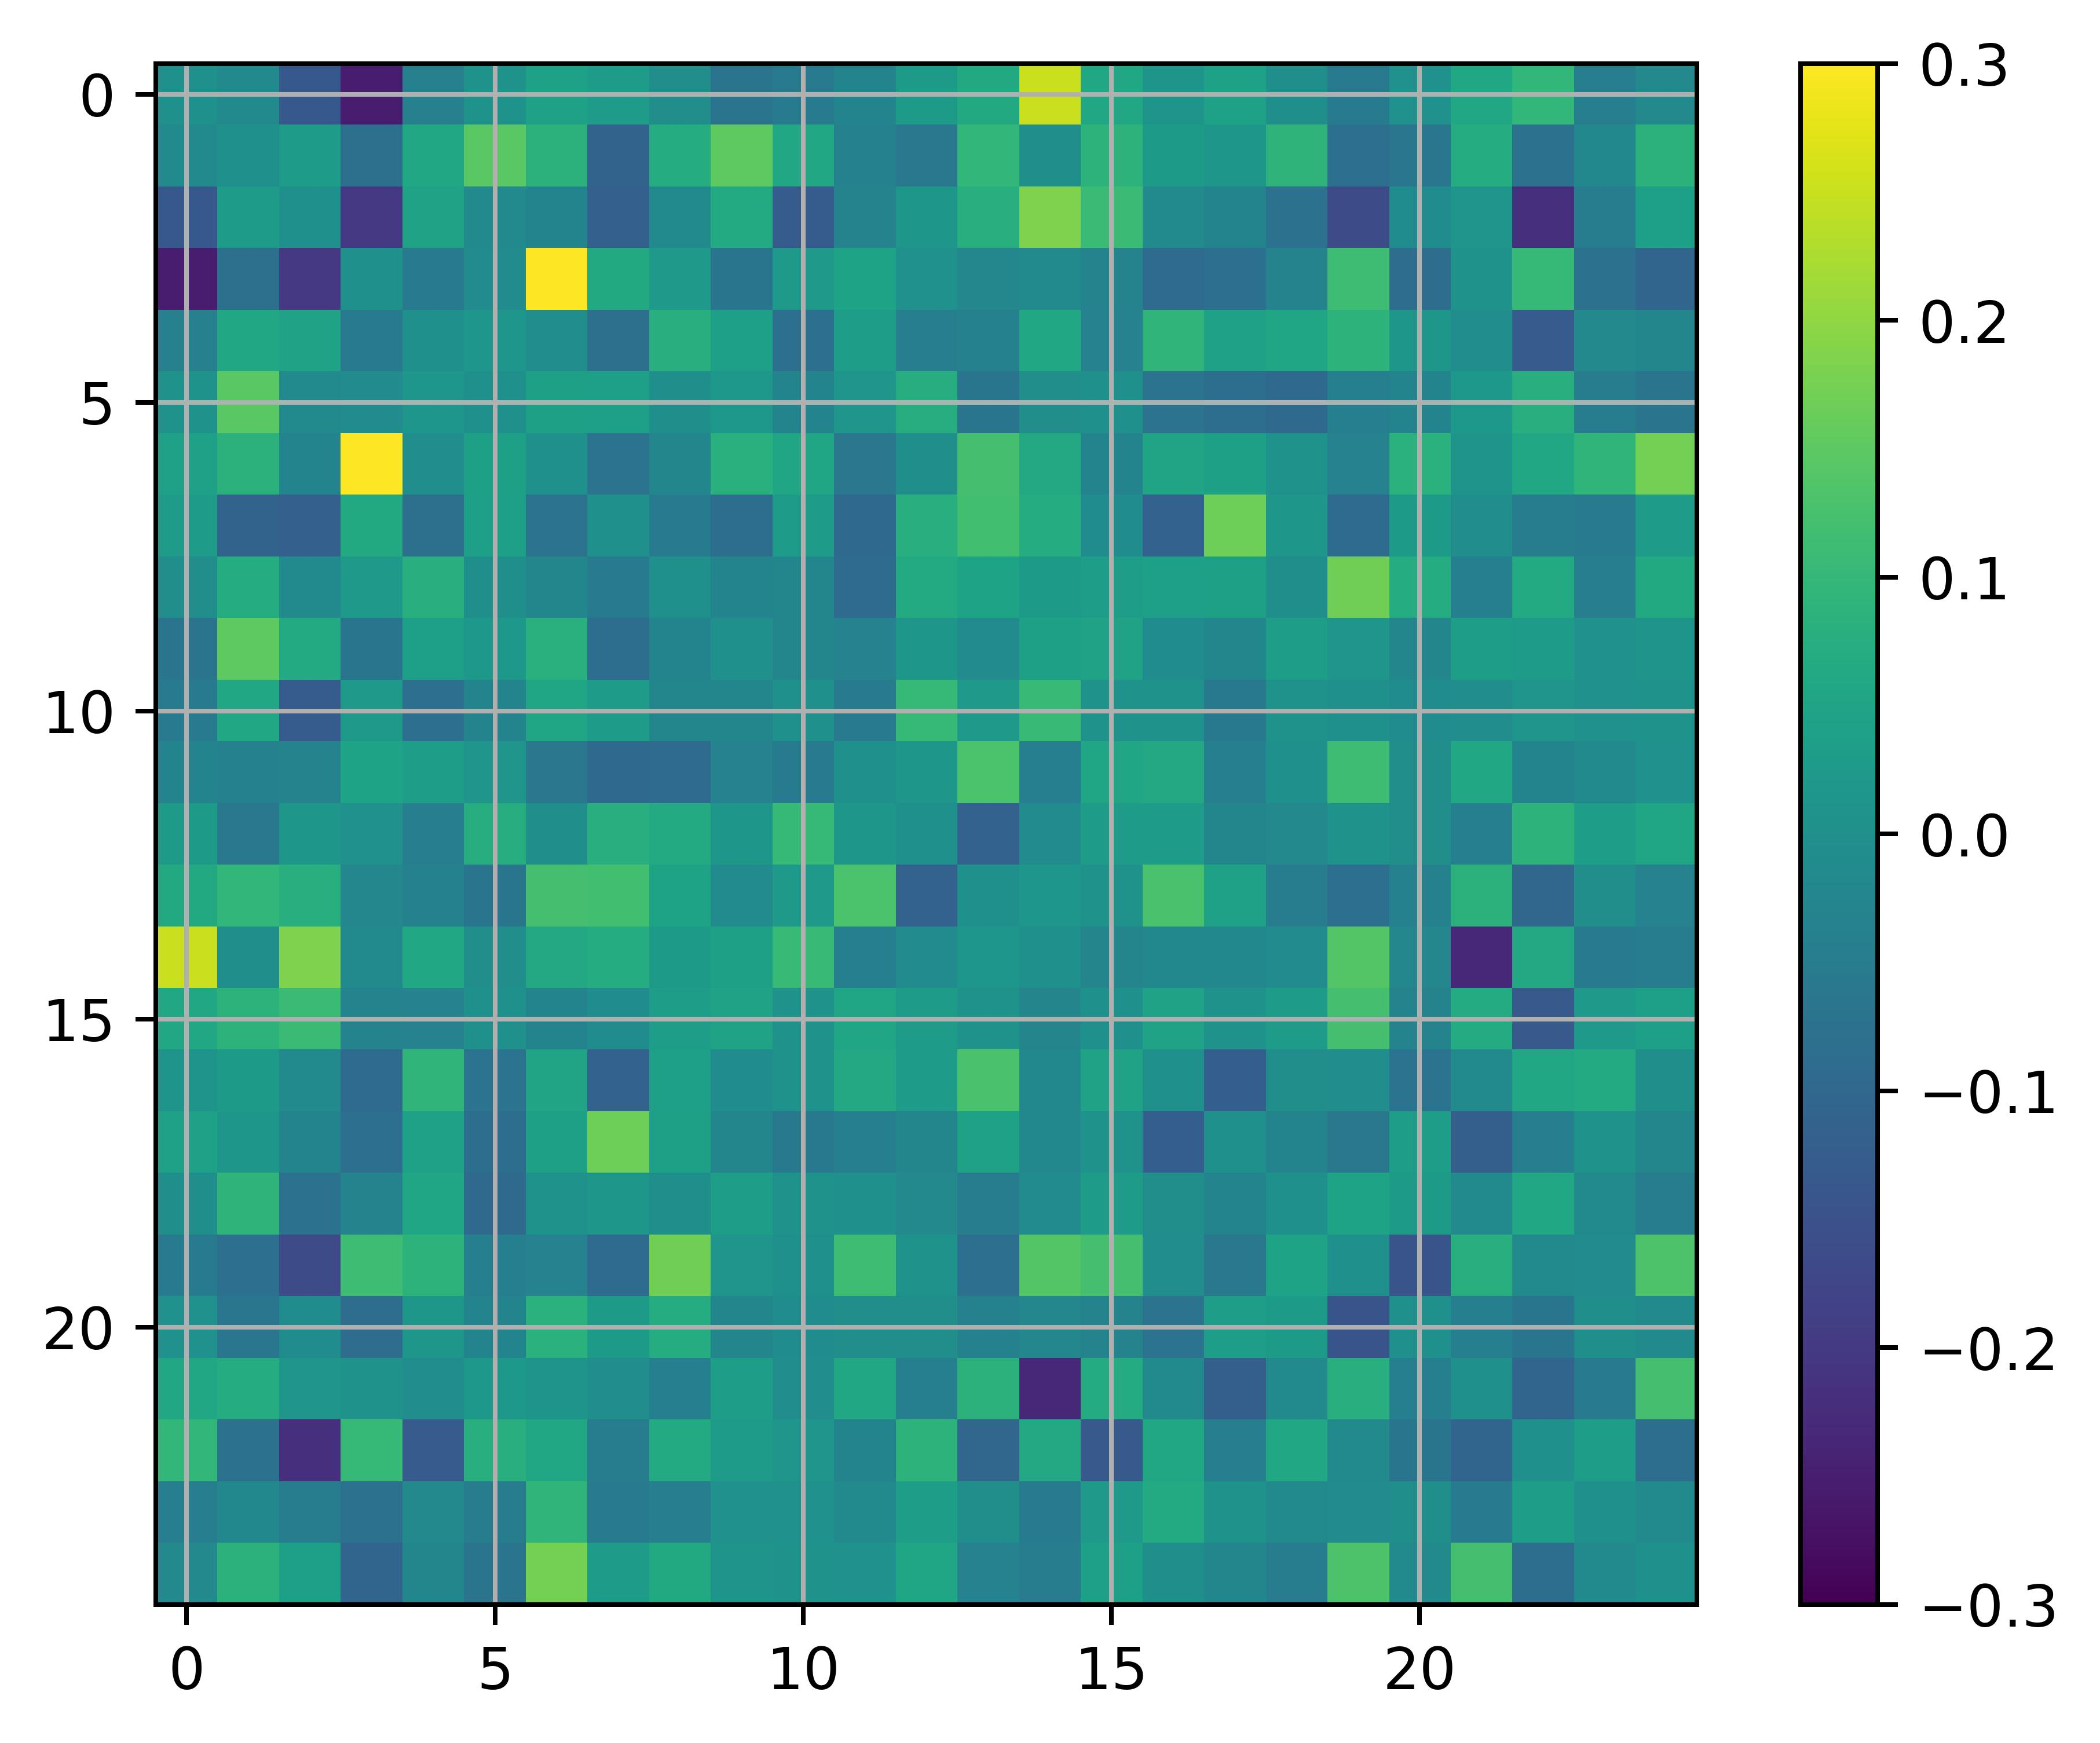
\includegraphics[width=0.2\textwidth]{../Analysis/DFC/size=480_step=180_rho=0.1/node=25_id=100206/c_16.jpg}
        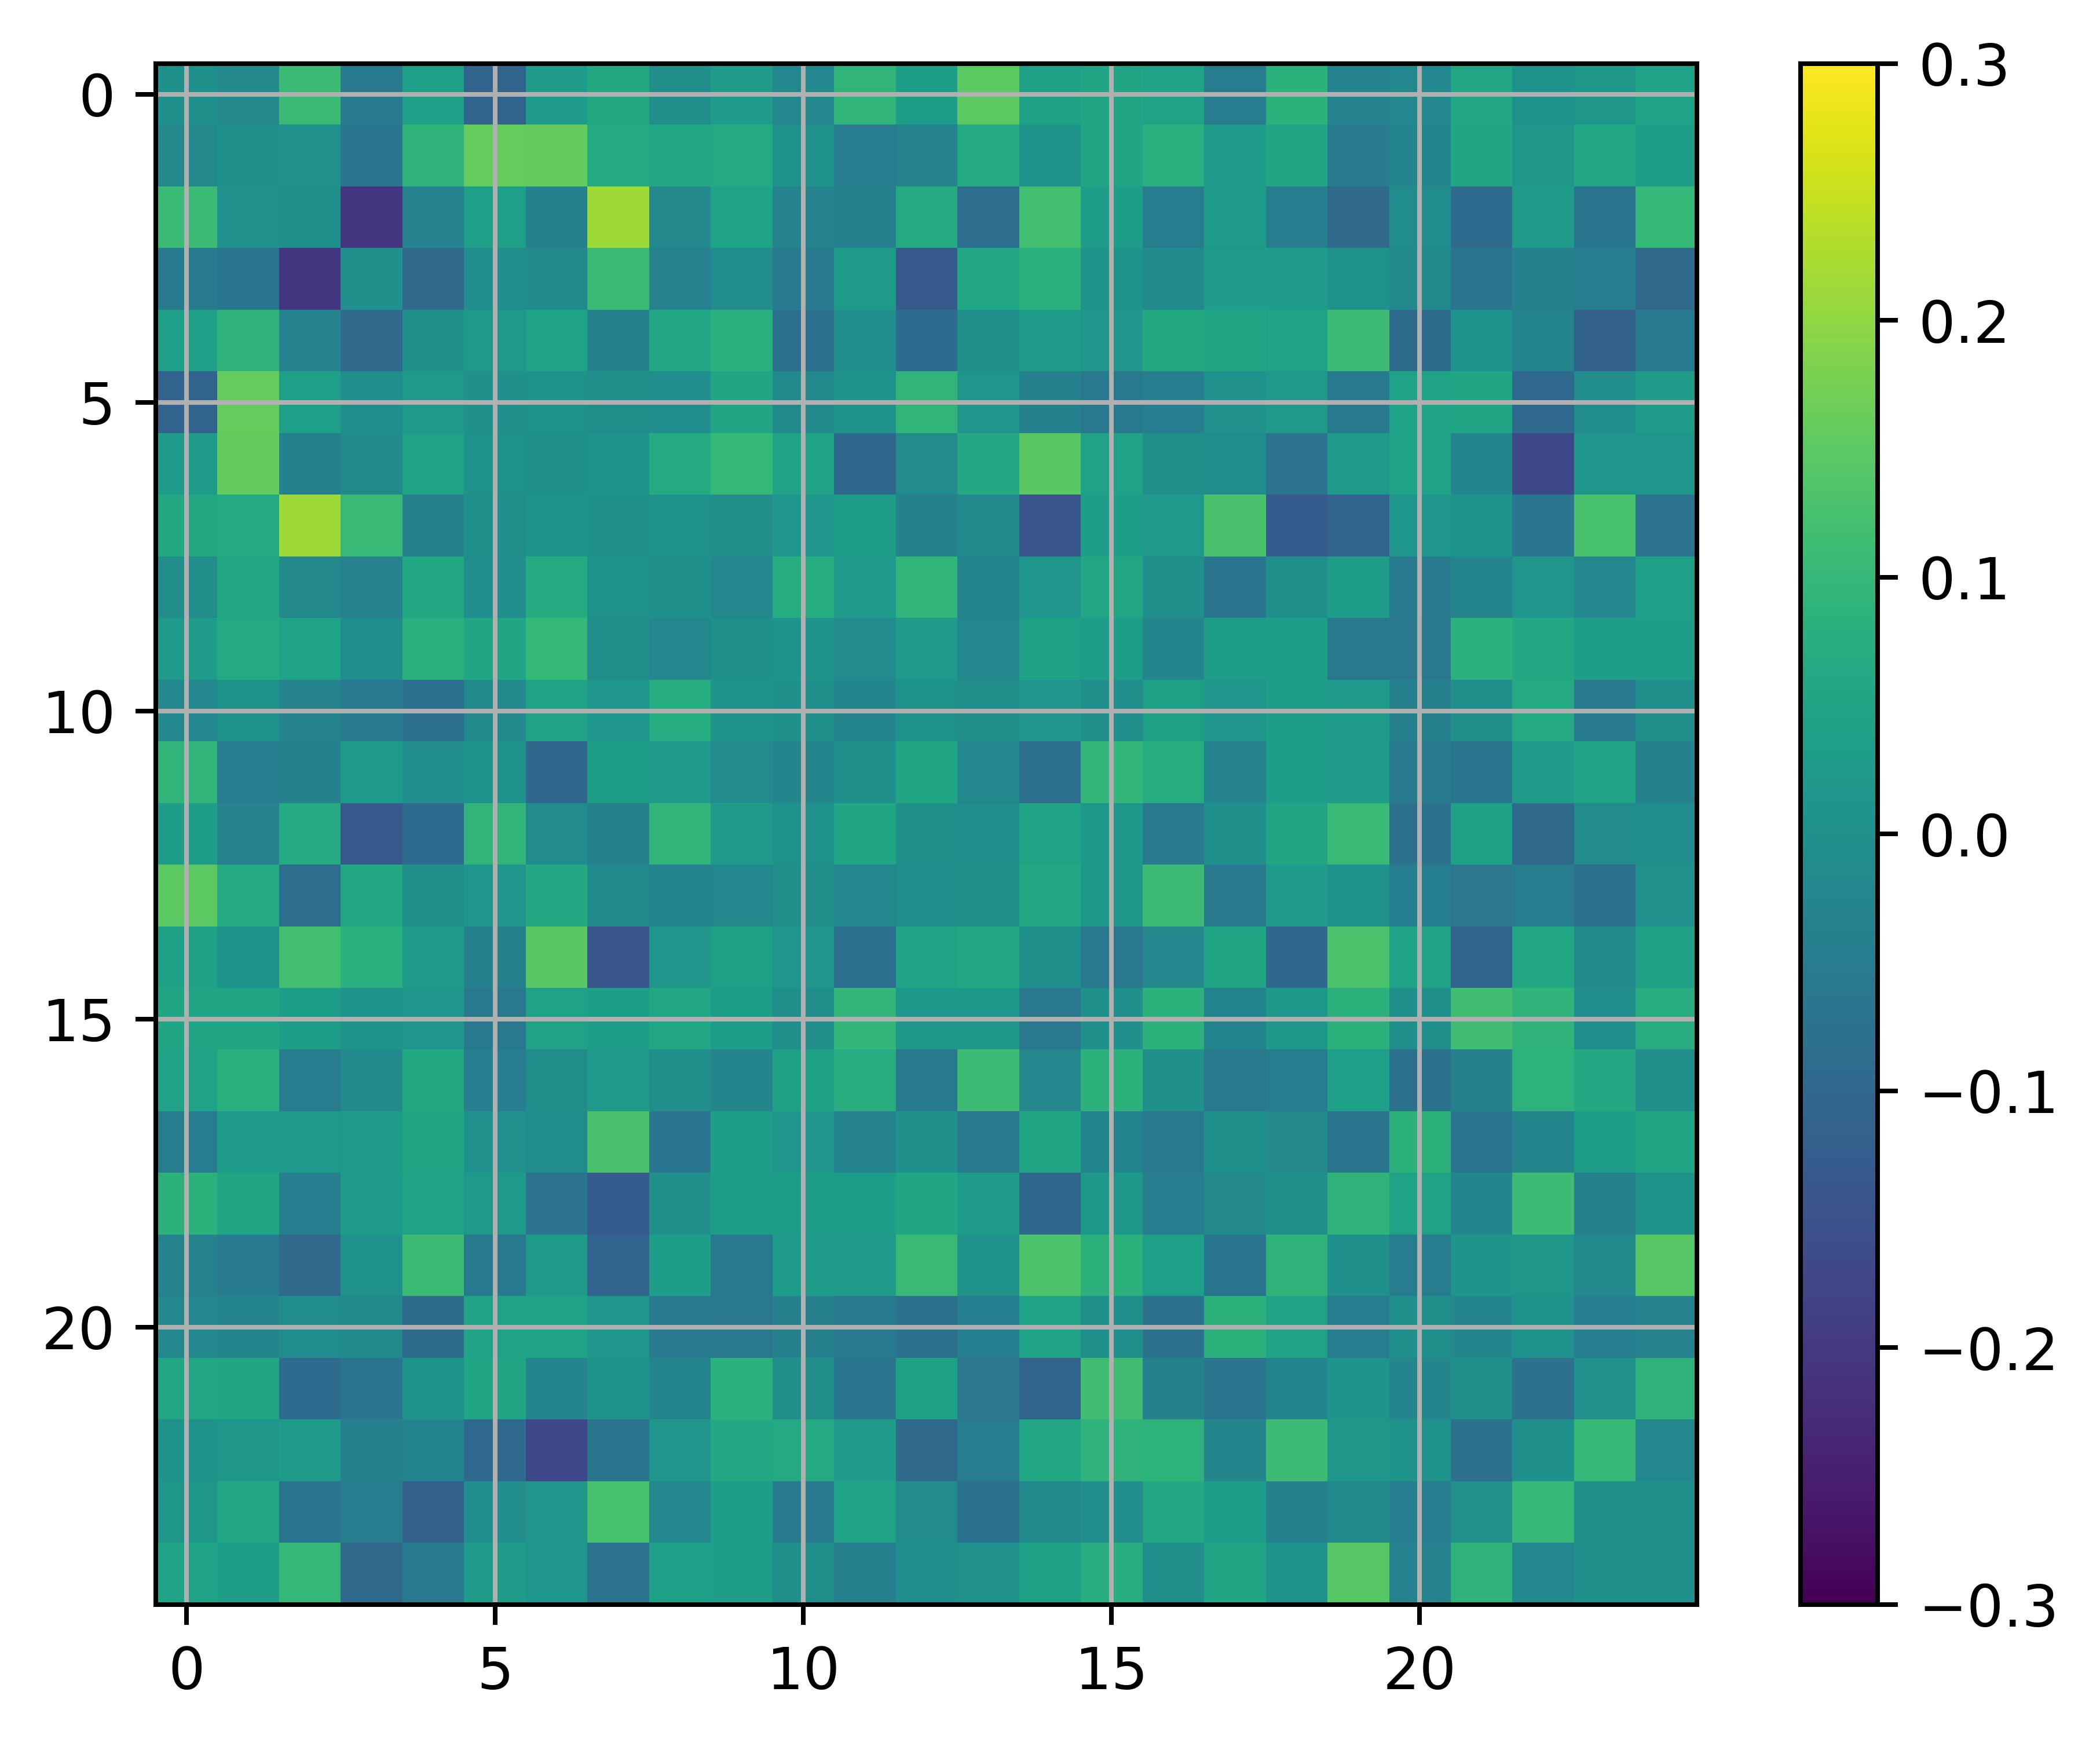
\includegraphics[width=0.2\textwidth]{../Analysis/DFC/size=480_step=180_rho=0.1/node=25_id=100206/c_18.jpg}
        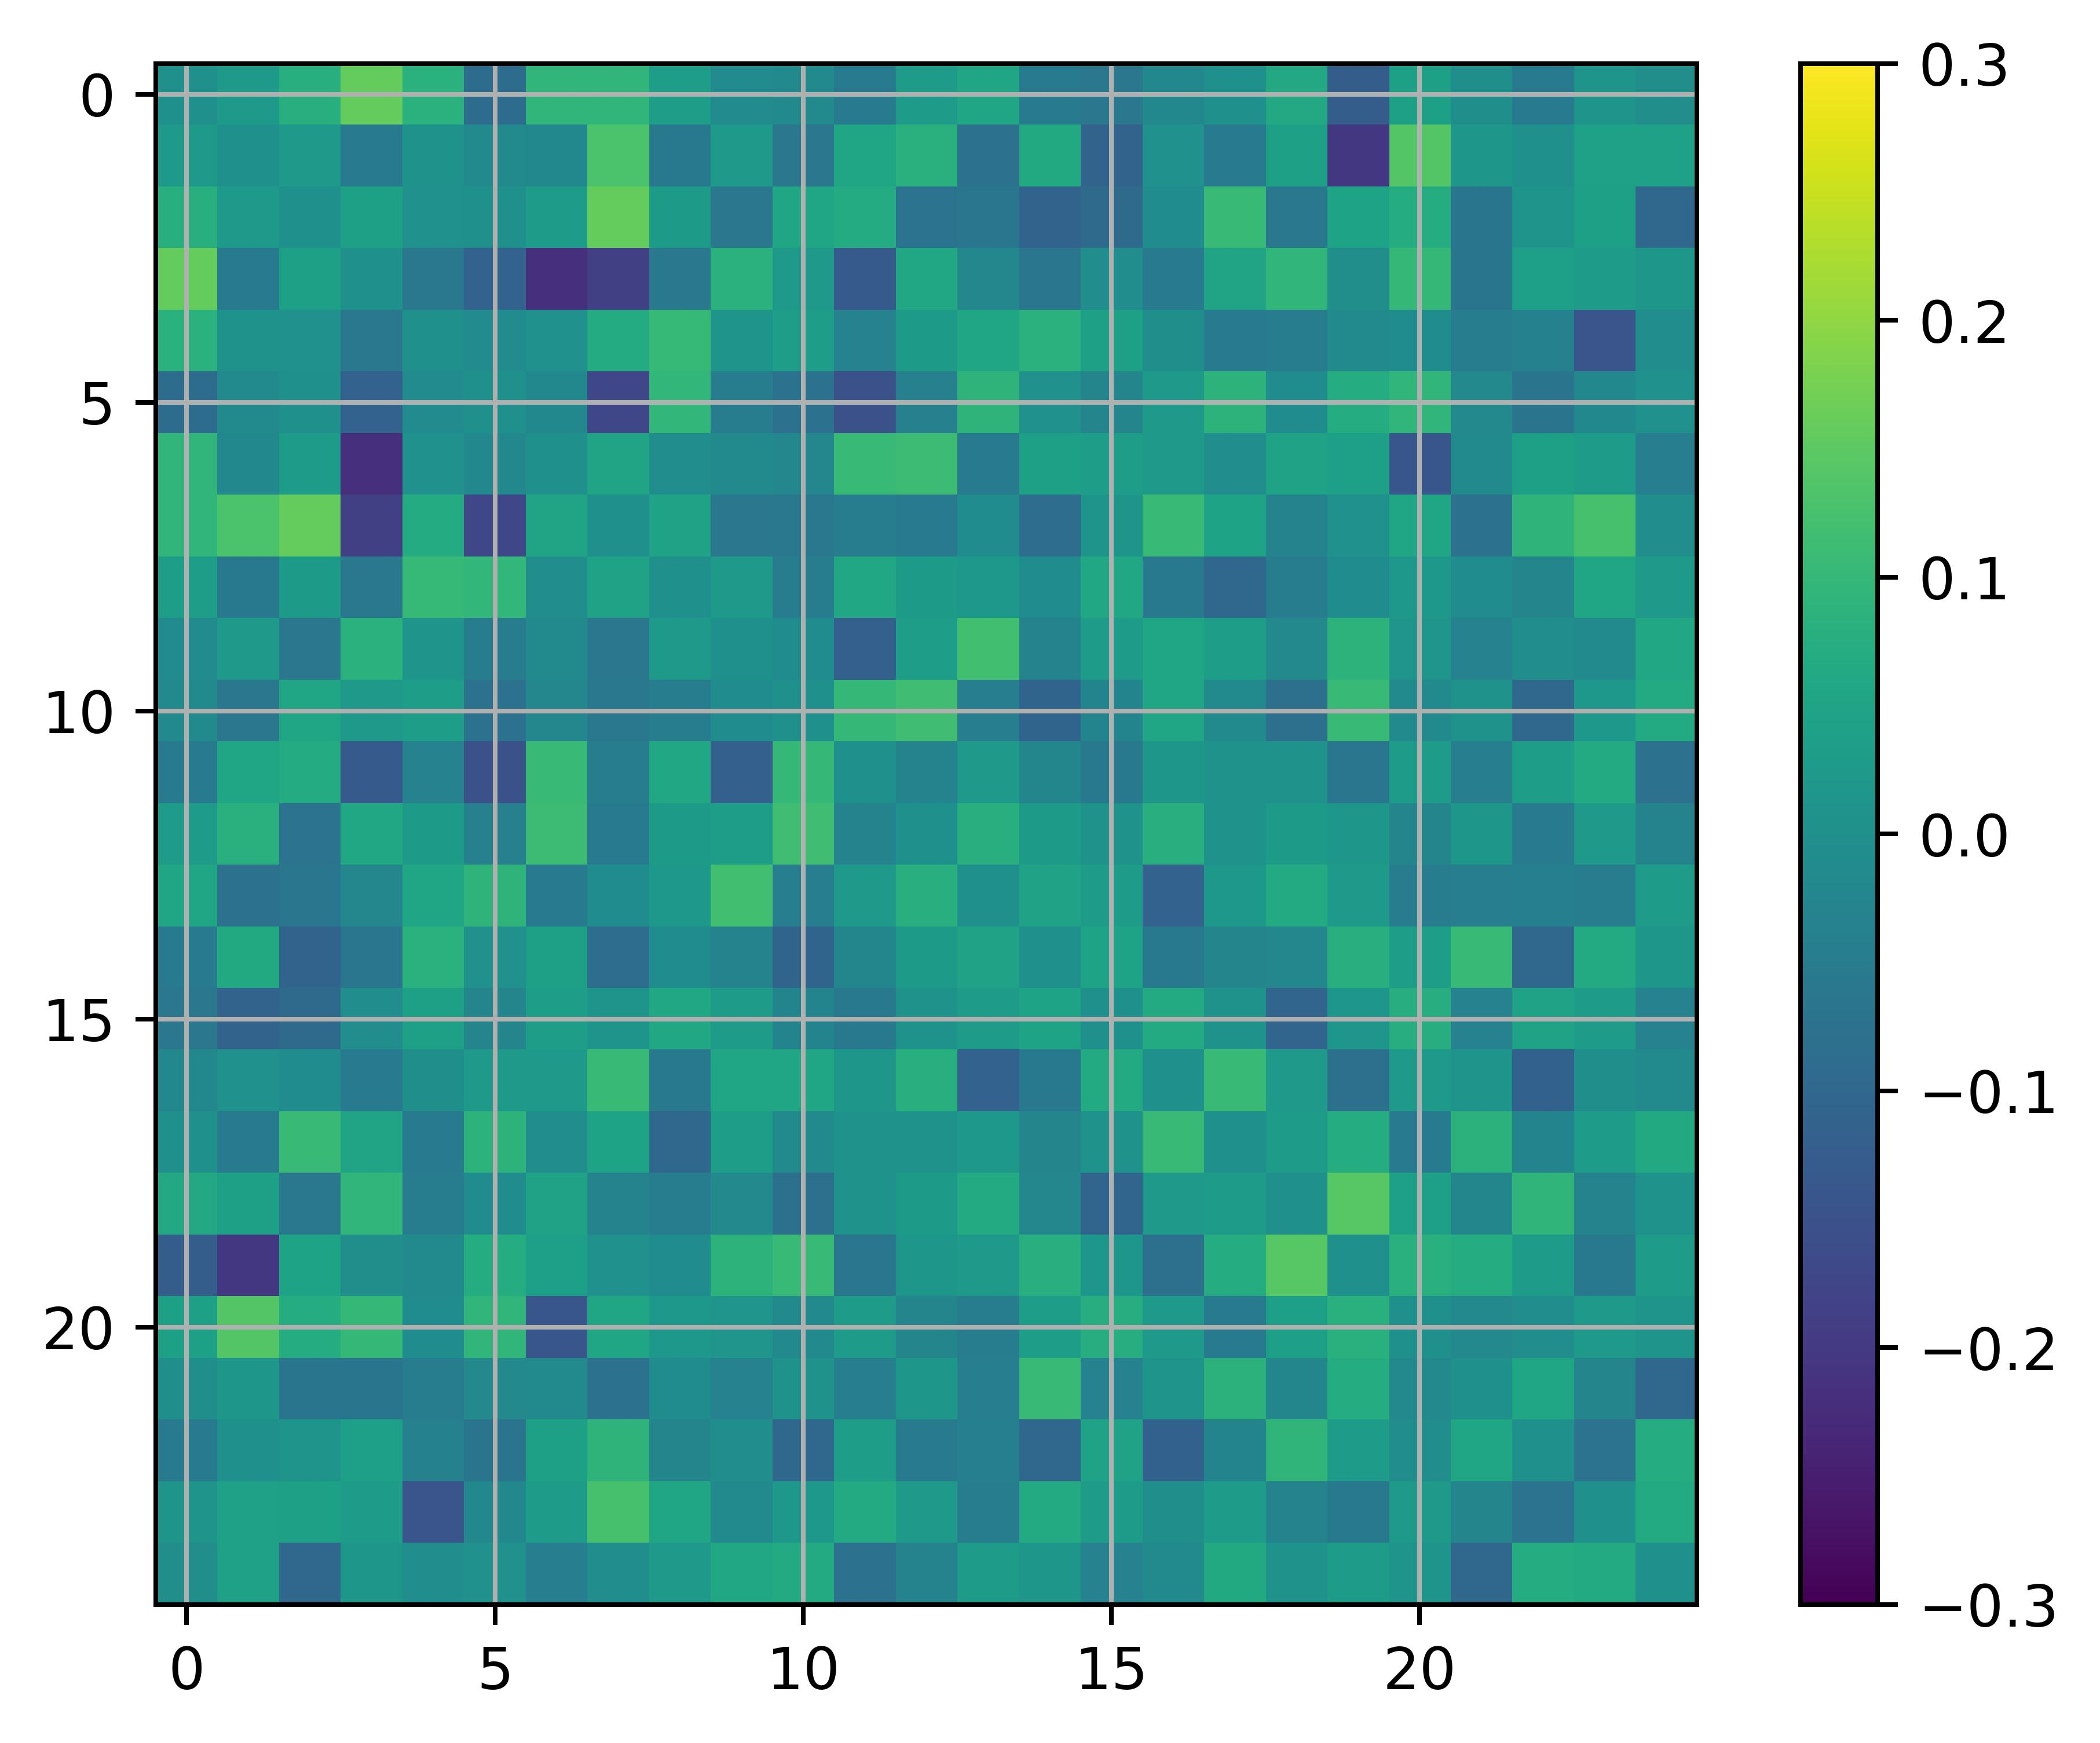
\includegraphics[width=0.2\textwidth]{../Analysis/DFC/size=480_step=180_rho=0.1/node=25_id=100206/c_20.jpg}
        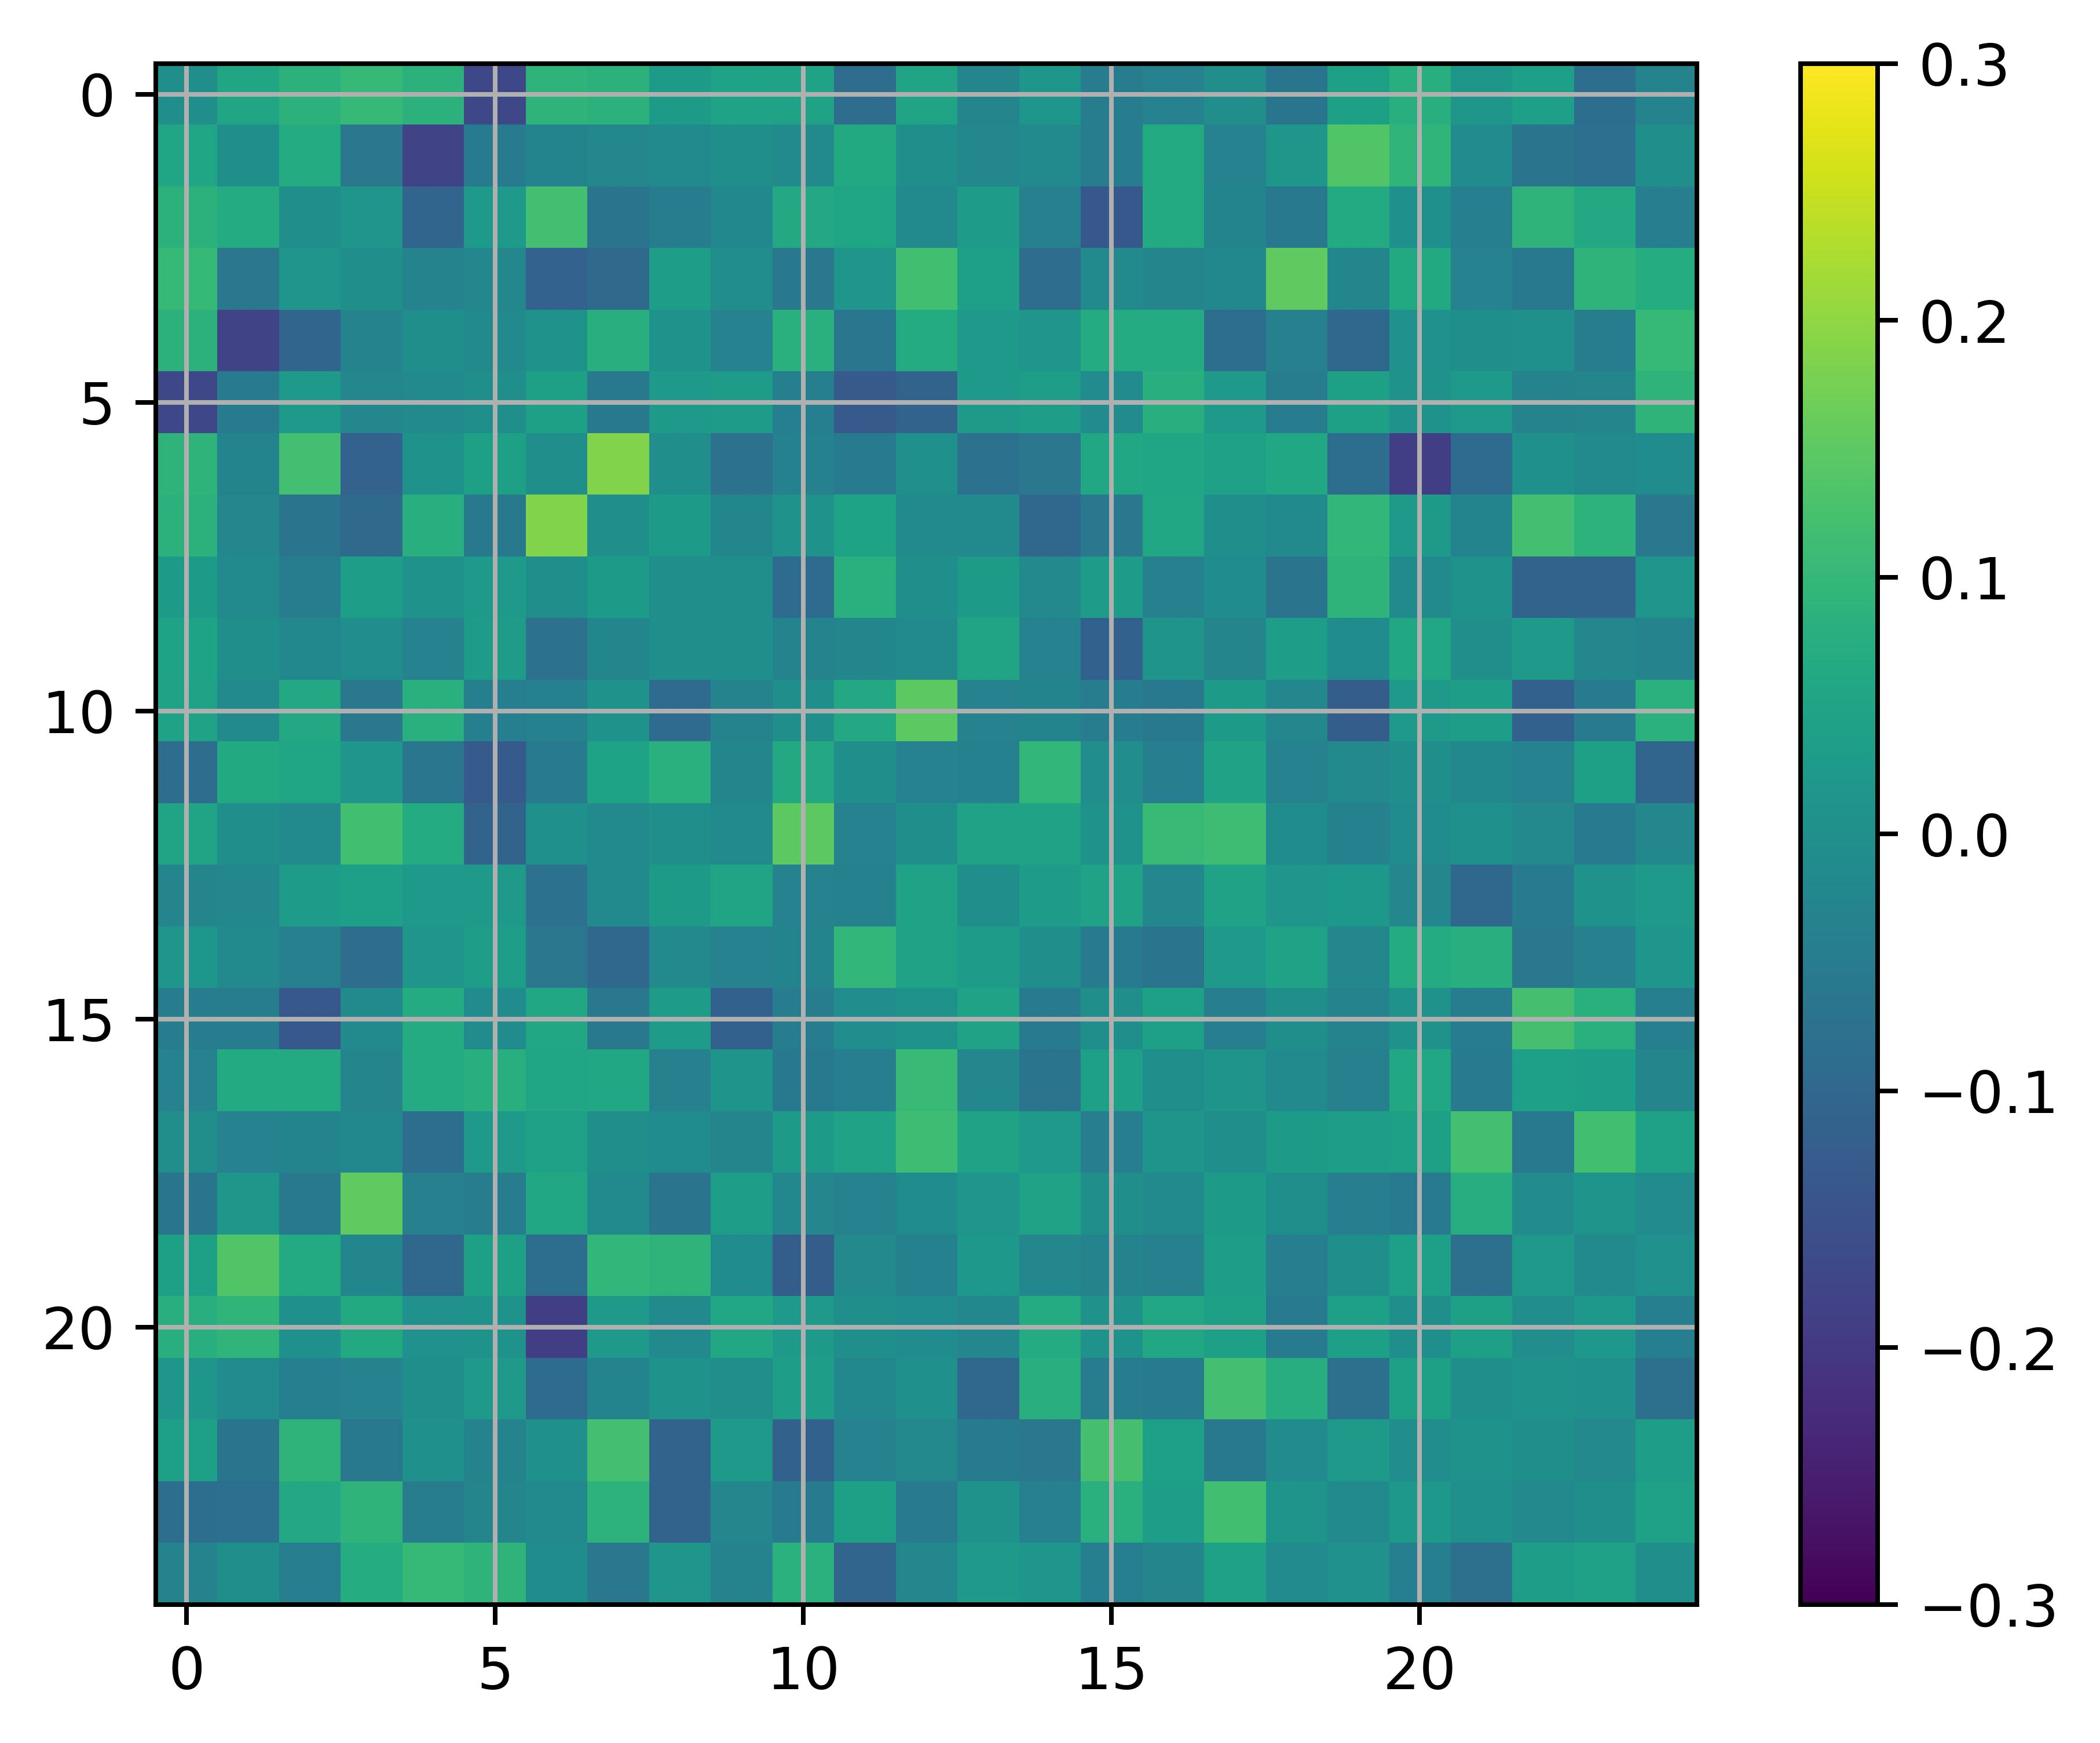
\includegraphics[width=0.2\textwidth]{../Analysis/DFC/size=480_step=180_rho=0.1/node=25_id=100206/c_22.jpg} \\
        \caption{Centered dynamic functional connectivity with $N_{node} = 25$.}
        % \label{LDA-example-1}
    \end{figure}

\end{frame}

\begin{frame}{Preprocessing - Examples}

    \begin{figure}[H]
        \centering
        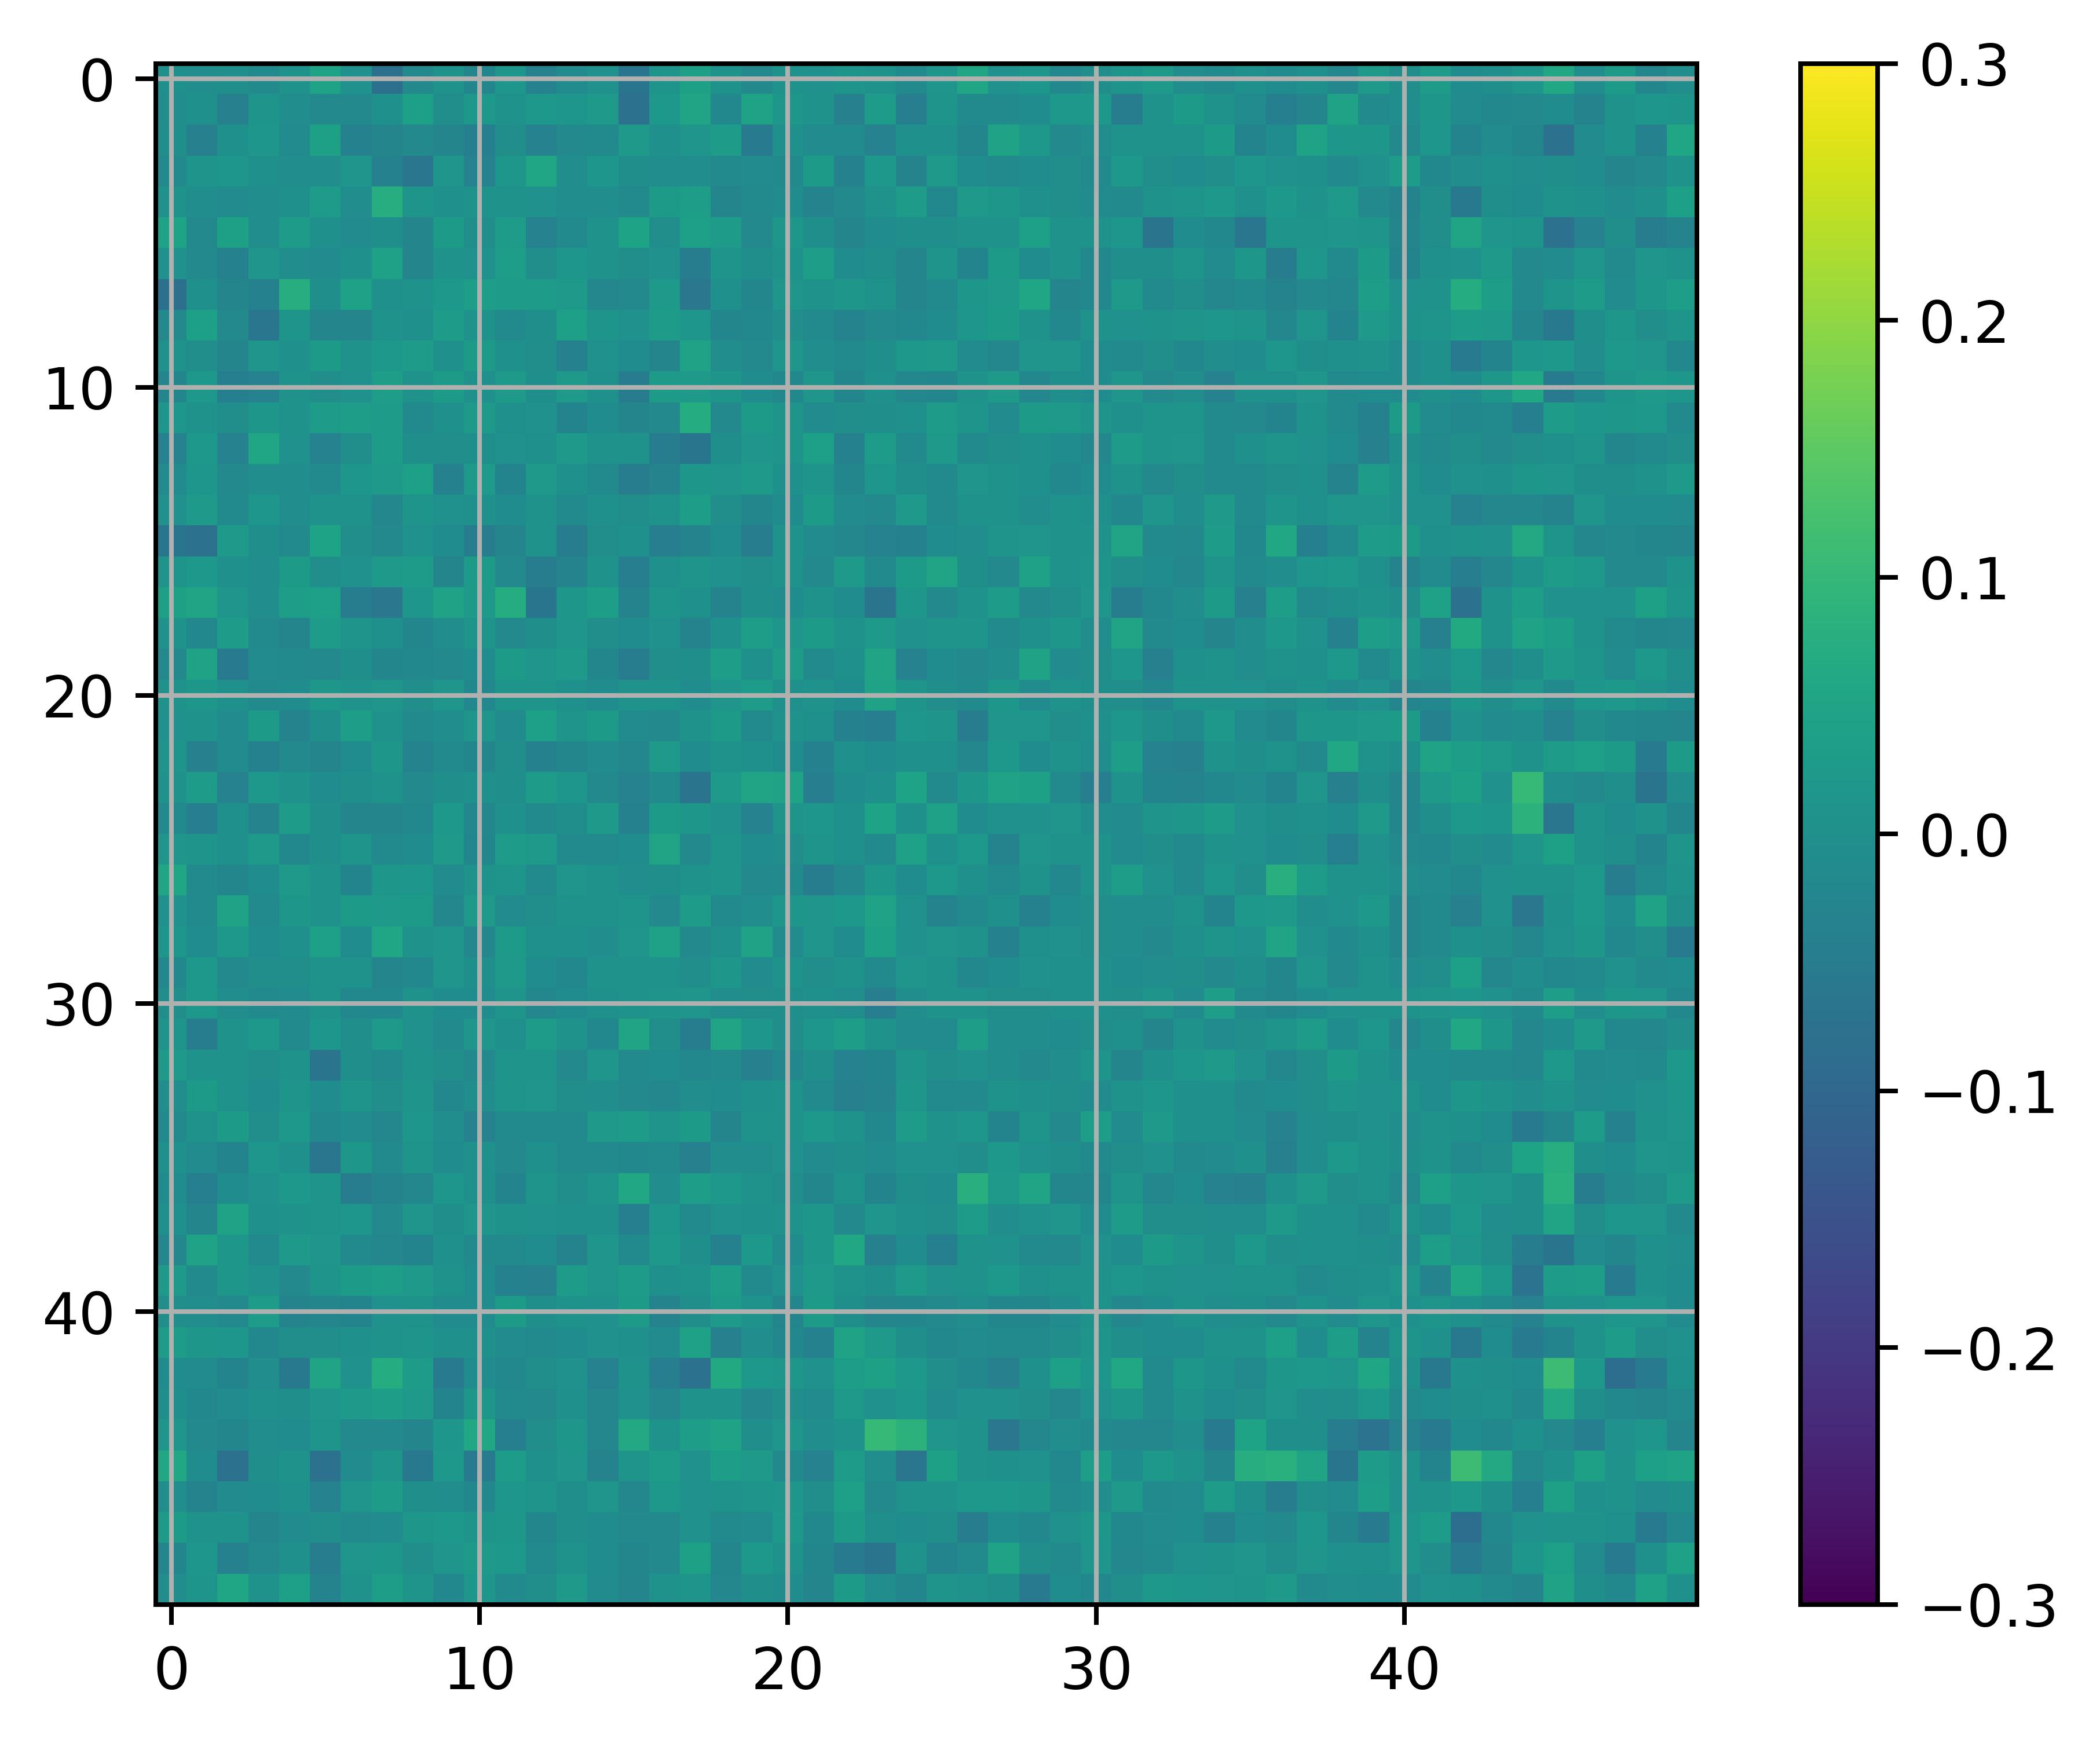
\includegraphics[width=0.2\textwidth]{../Analysis/DFC/size=480_step=180_rho=0.1/node=50_id=100206/c_0.jpg}
        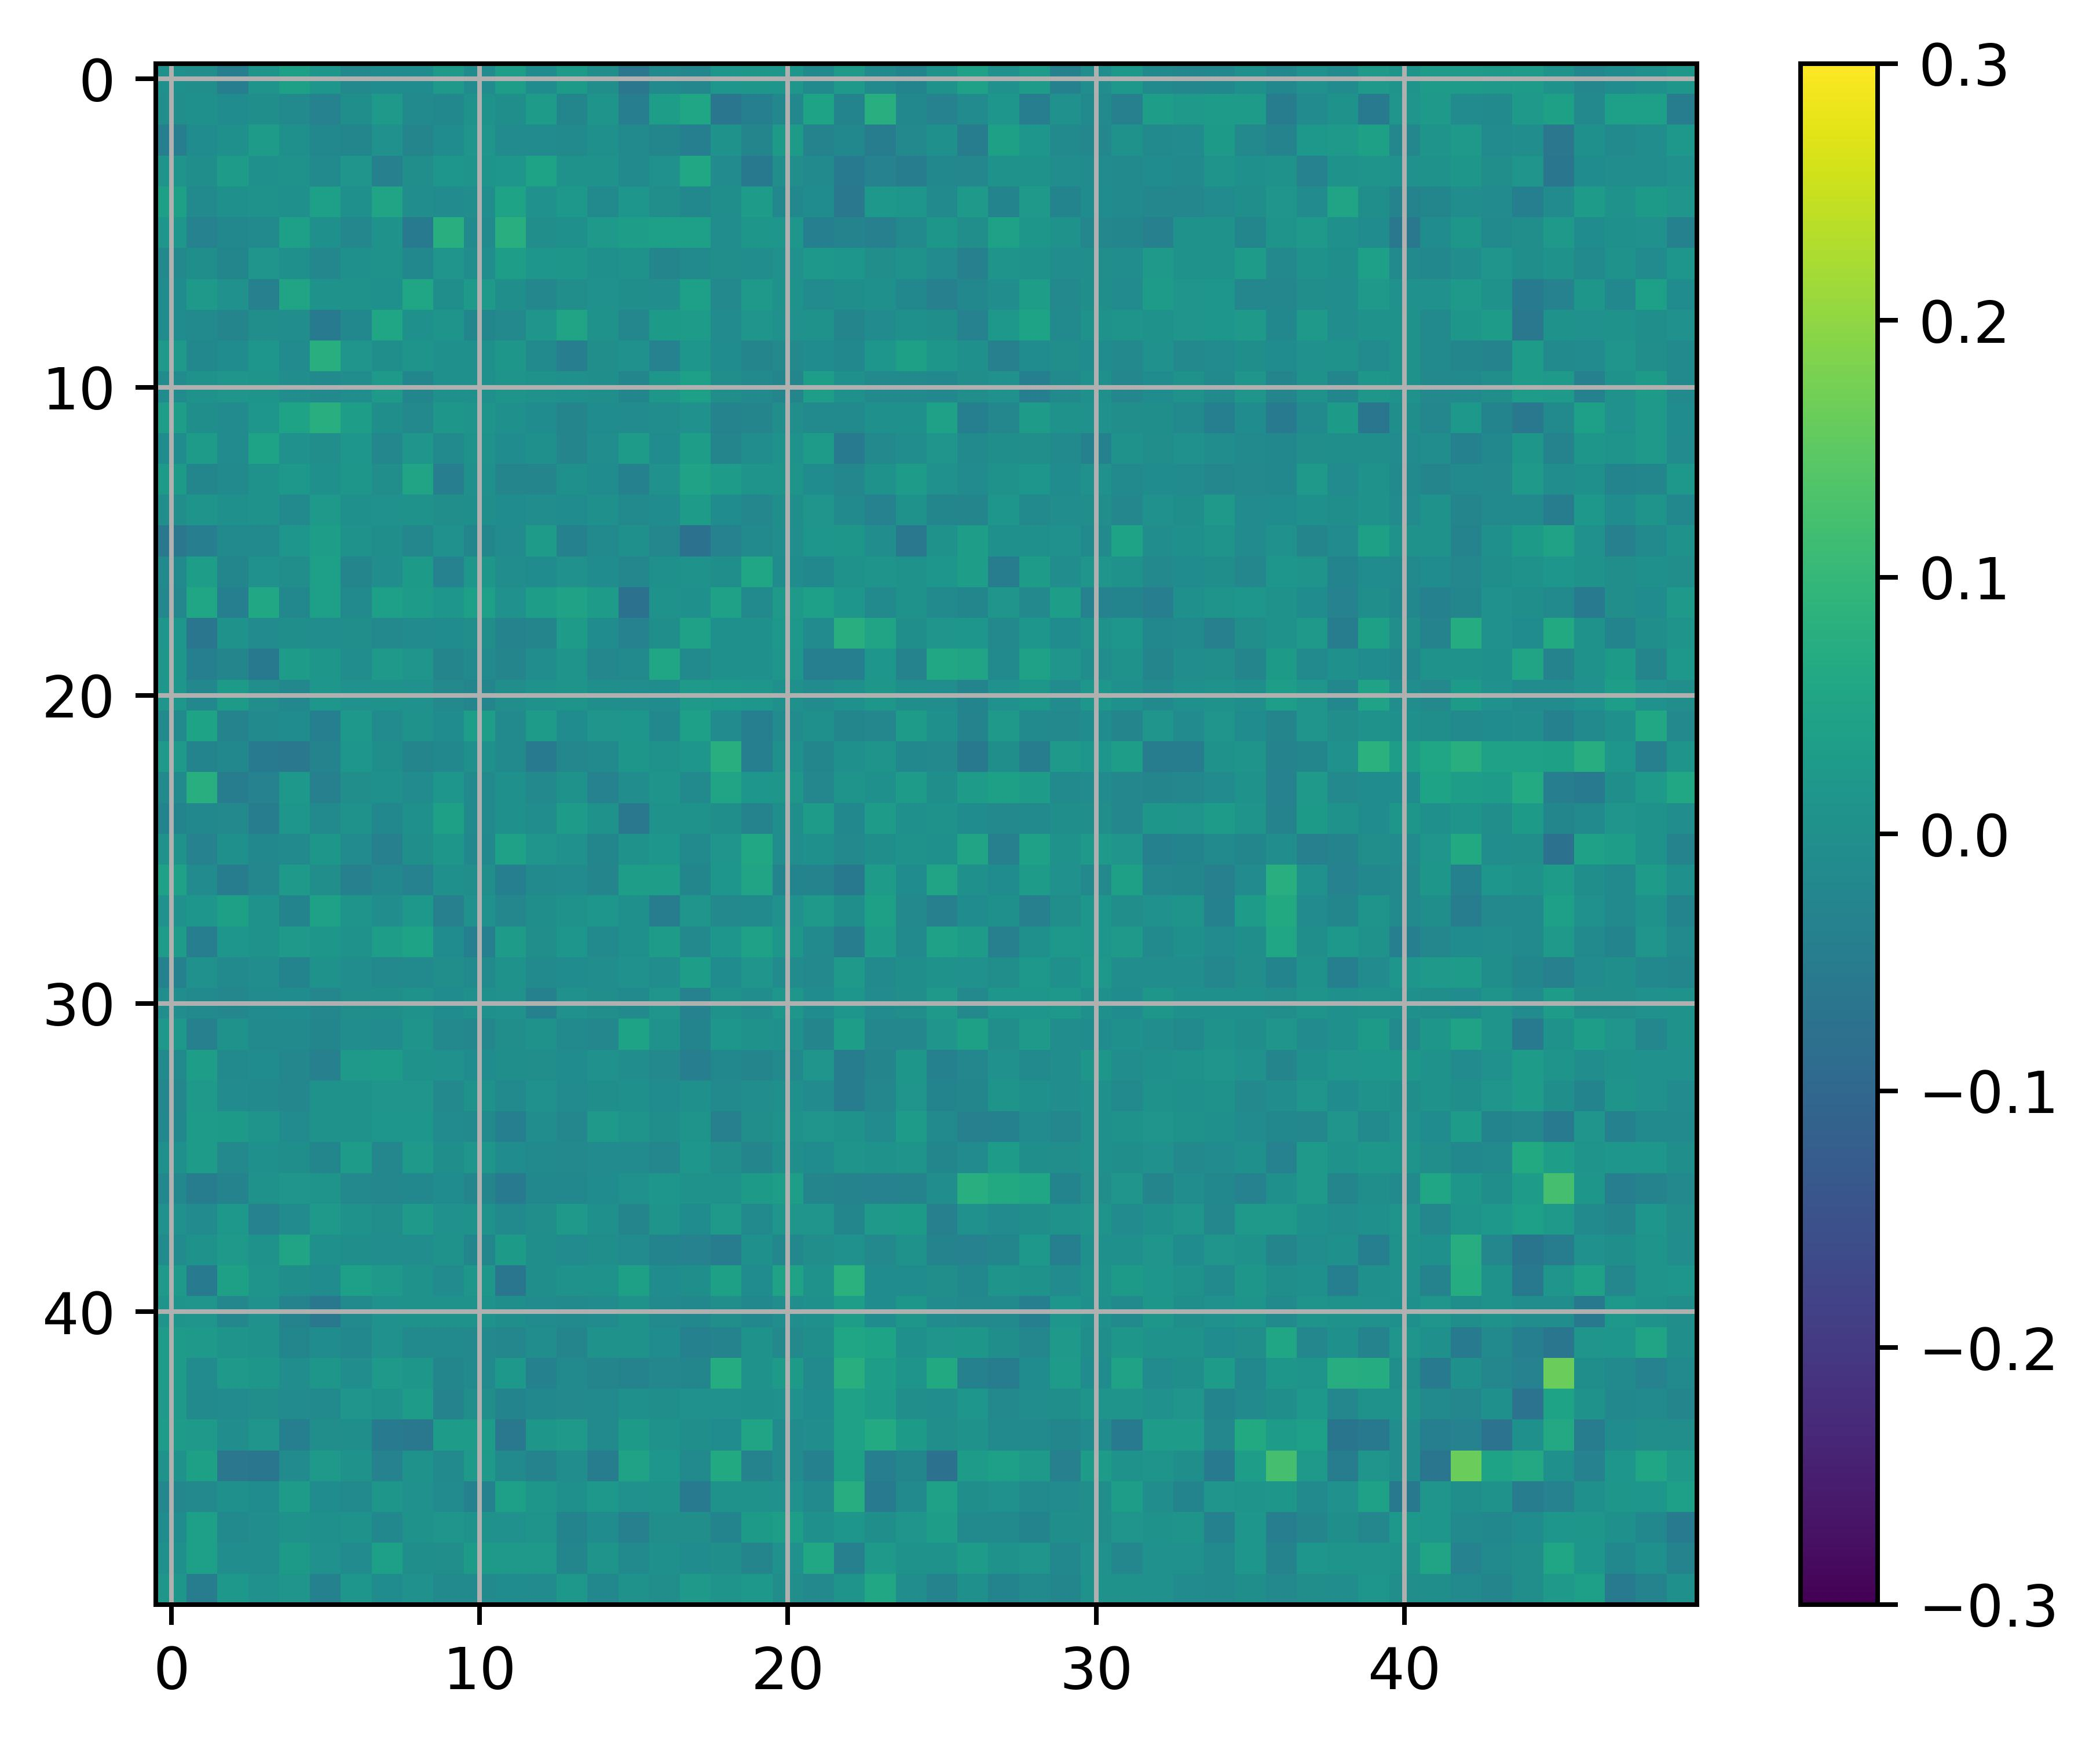
\includegraphics[width=0.2\textwidth]{../Analysis/DFC/size=480_step=180_rho=0.1/node=50_id=100206/c_2.jpg}
        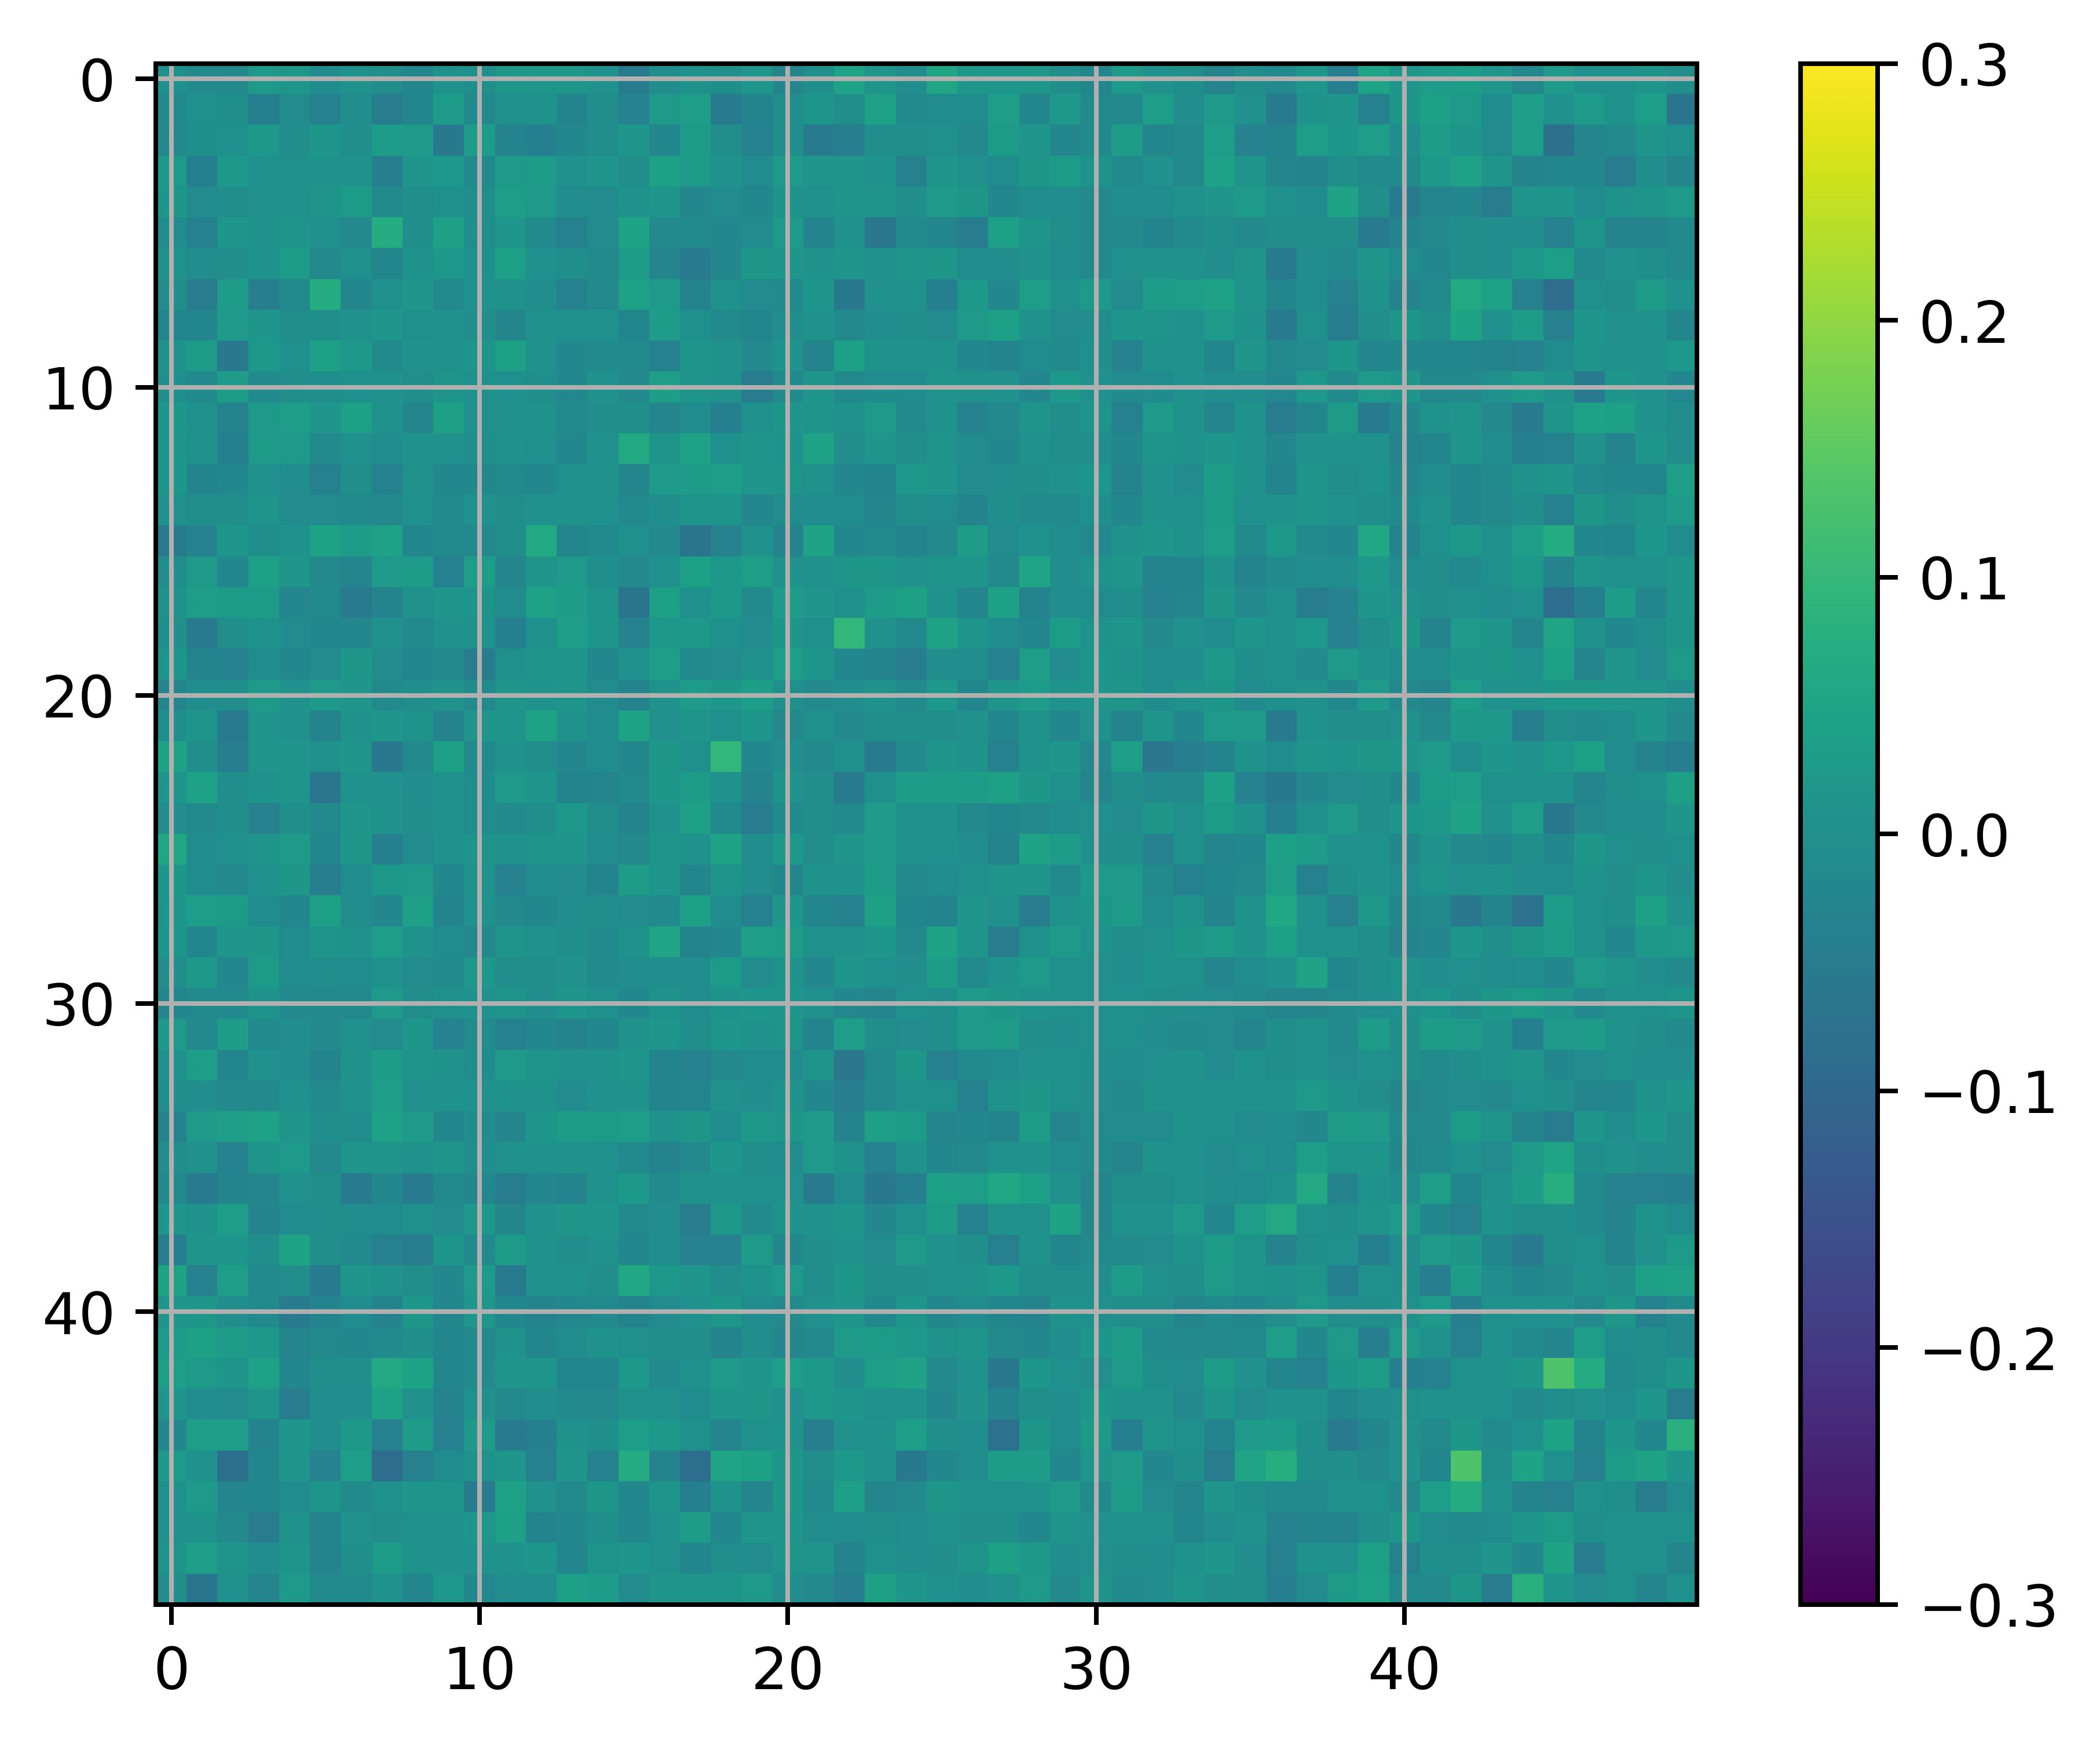
\includegraphics[width=0.2\textwidth]{../Analysis/DFC/size=480_step=180_rho=0.1/node=50_id=100206/c_4.jpg}
        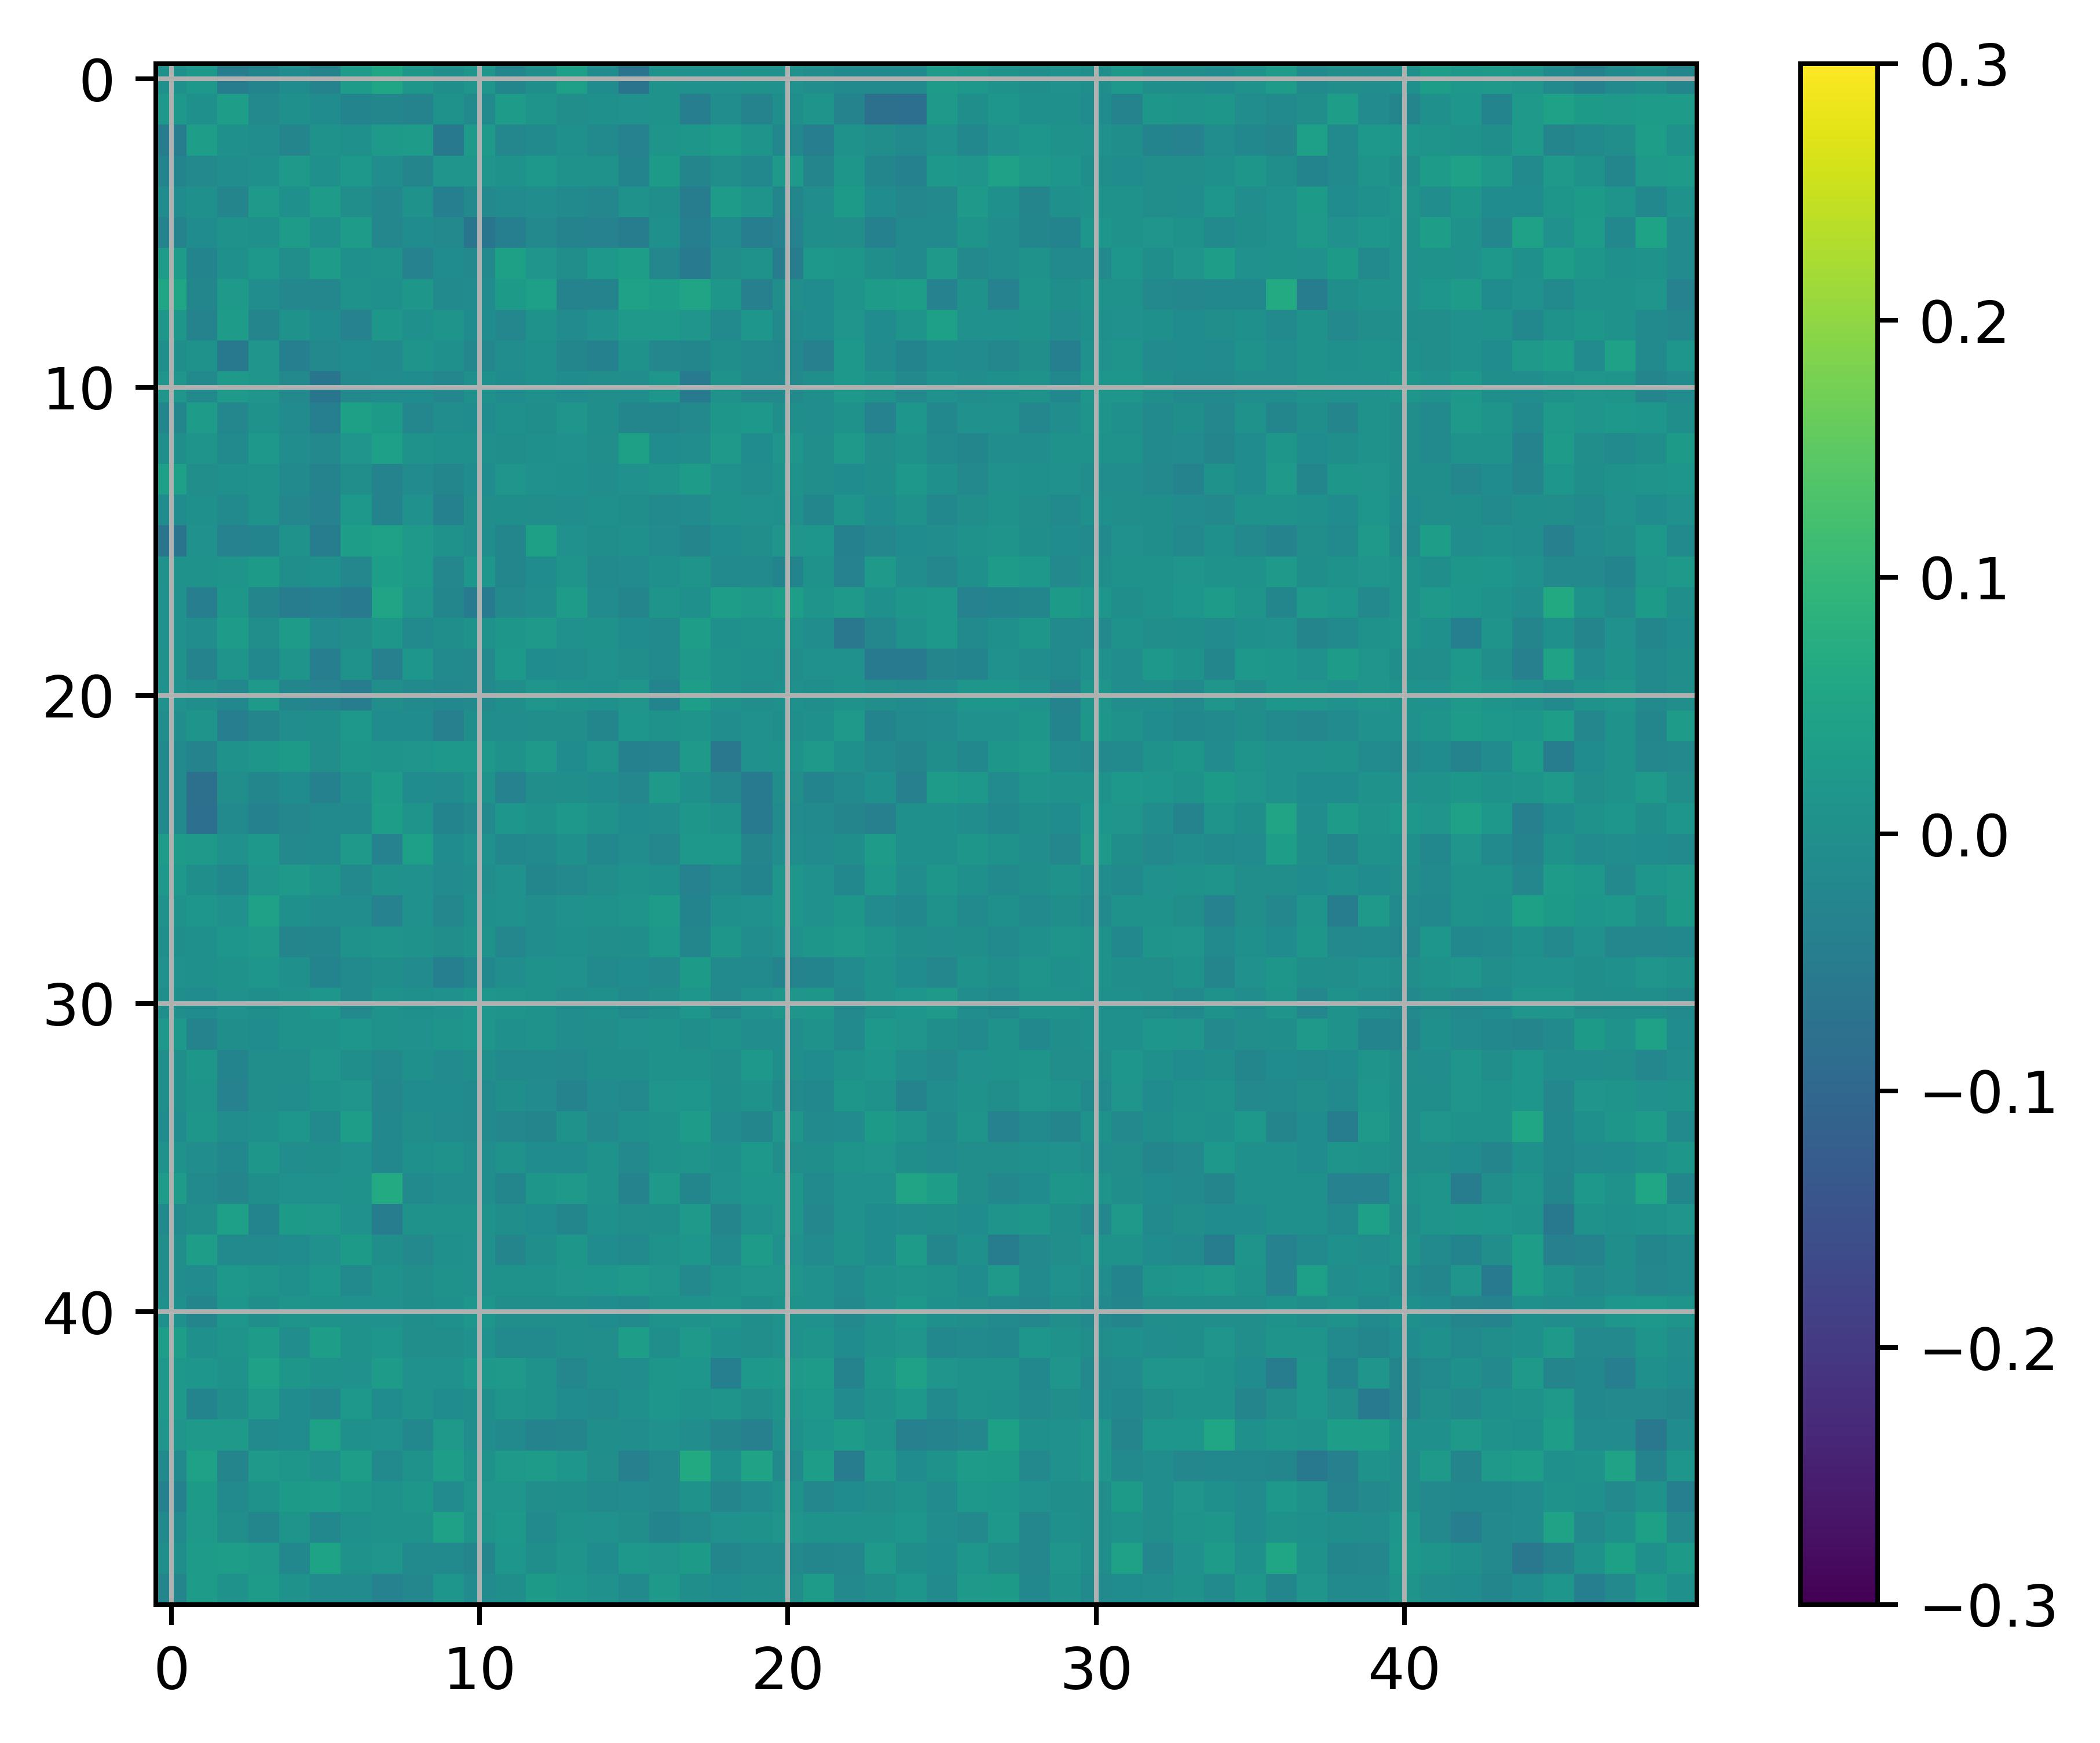
\includegraphics[width=0.2\textwidth]{../Analysis/DFC/size=480_step=180_rho=0.1/node=50_id=100206/c_6.jpg} \\
        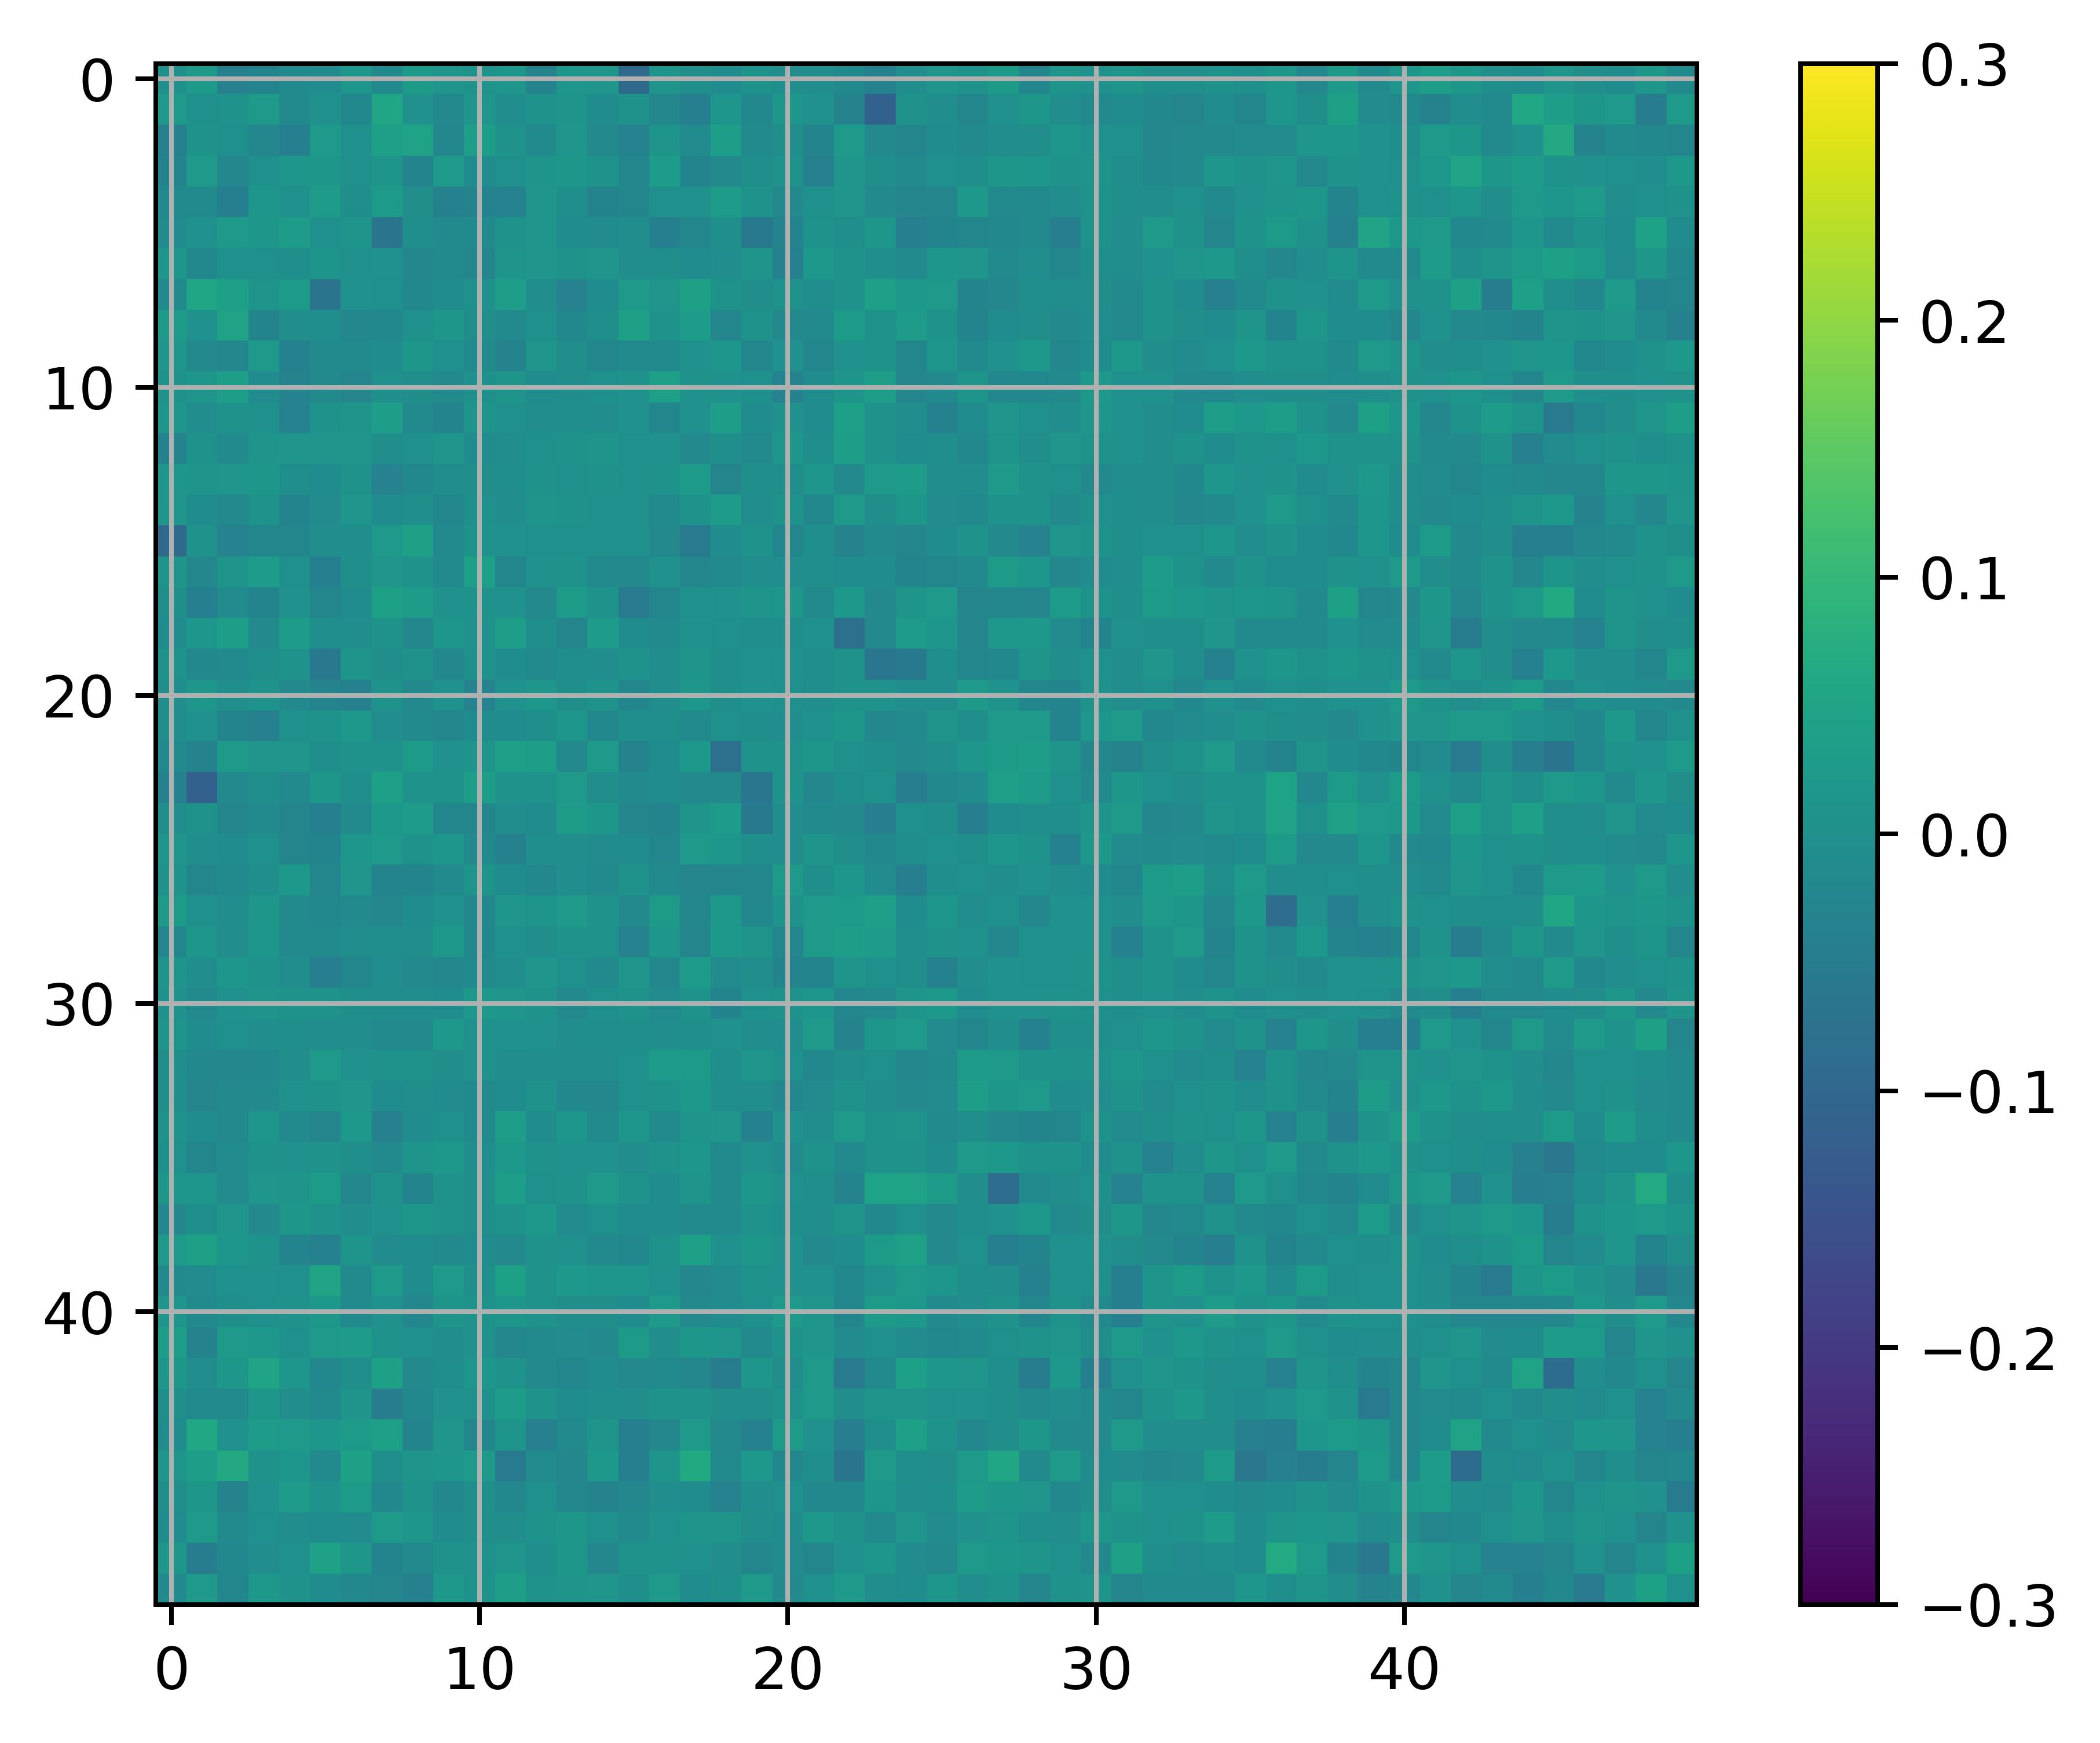
\includegraphics[width=0.2\textwidth]{../Analysis/DFC/size=480_step=180_rho=0.1/node=50_id=100206/c_8.jpg}
        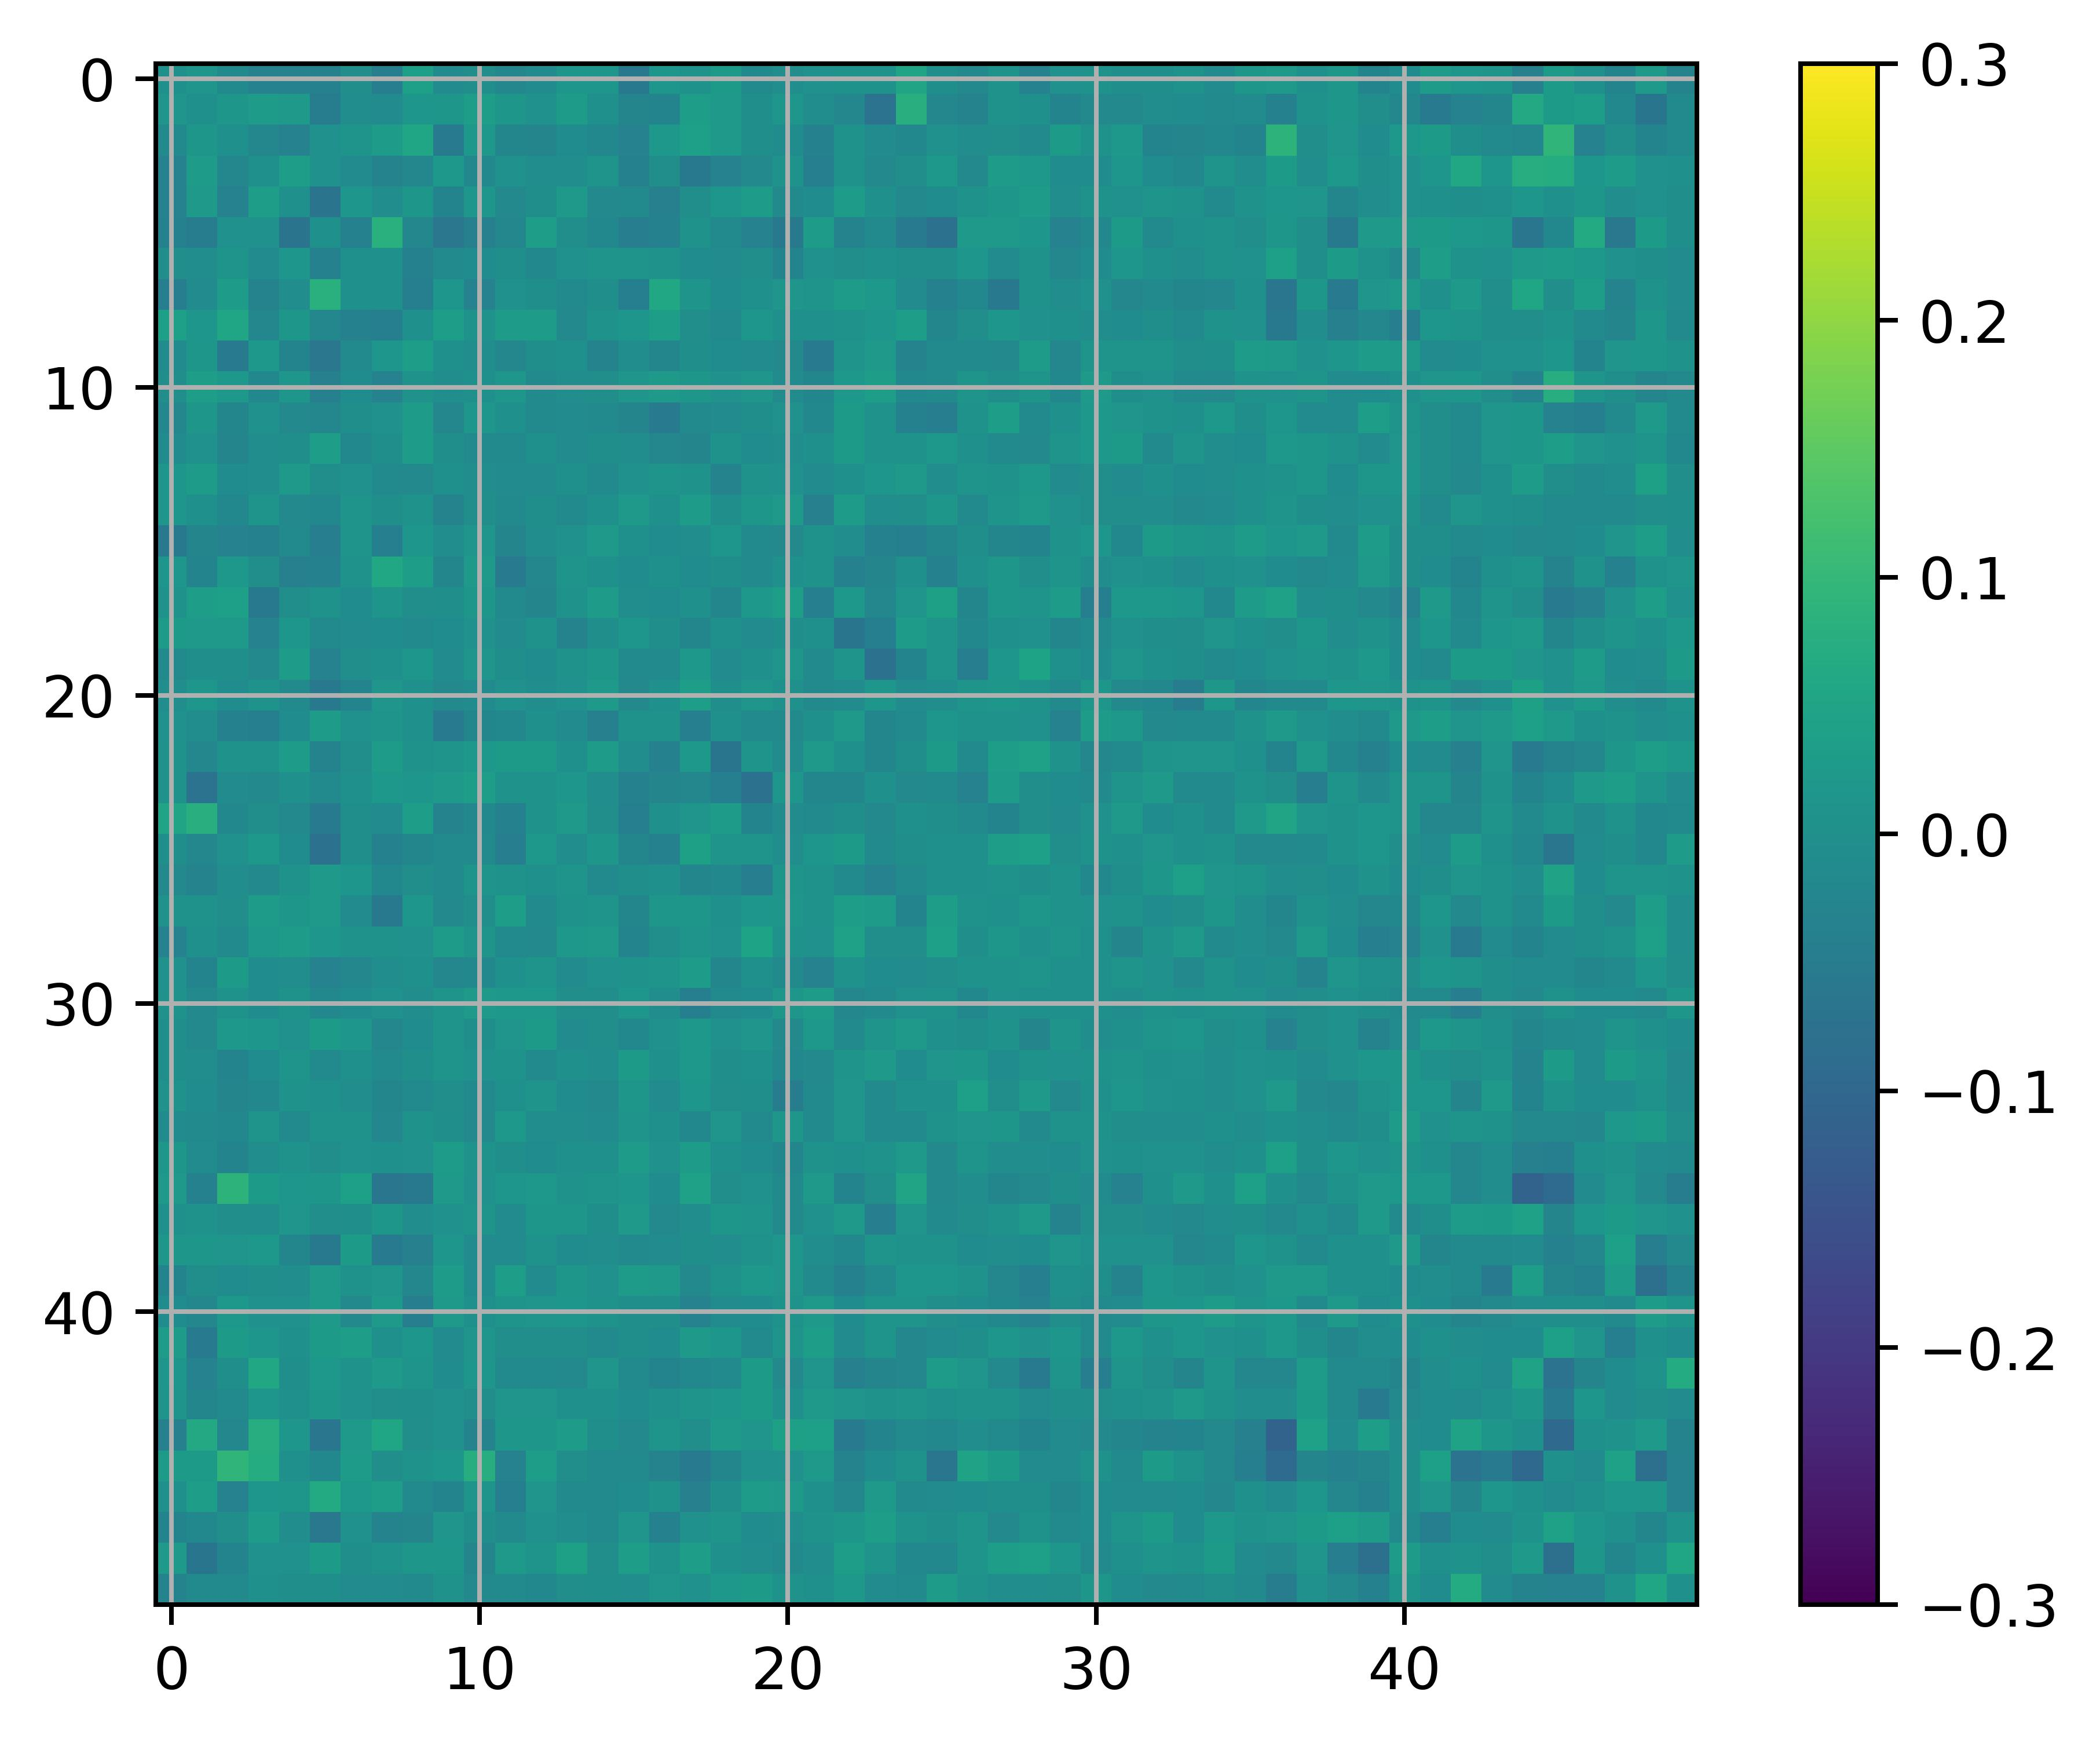
\includegraphics[width=0.2\textwidth]{../Analysis/DFC/size=480_step=180_rho=0.1/node=50_id=100206/c_10.jpg}
        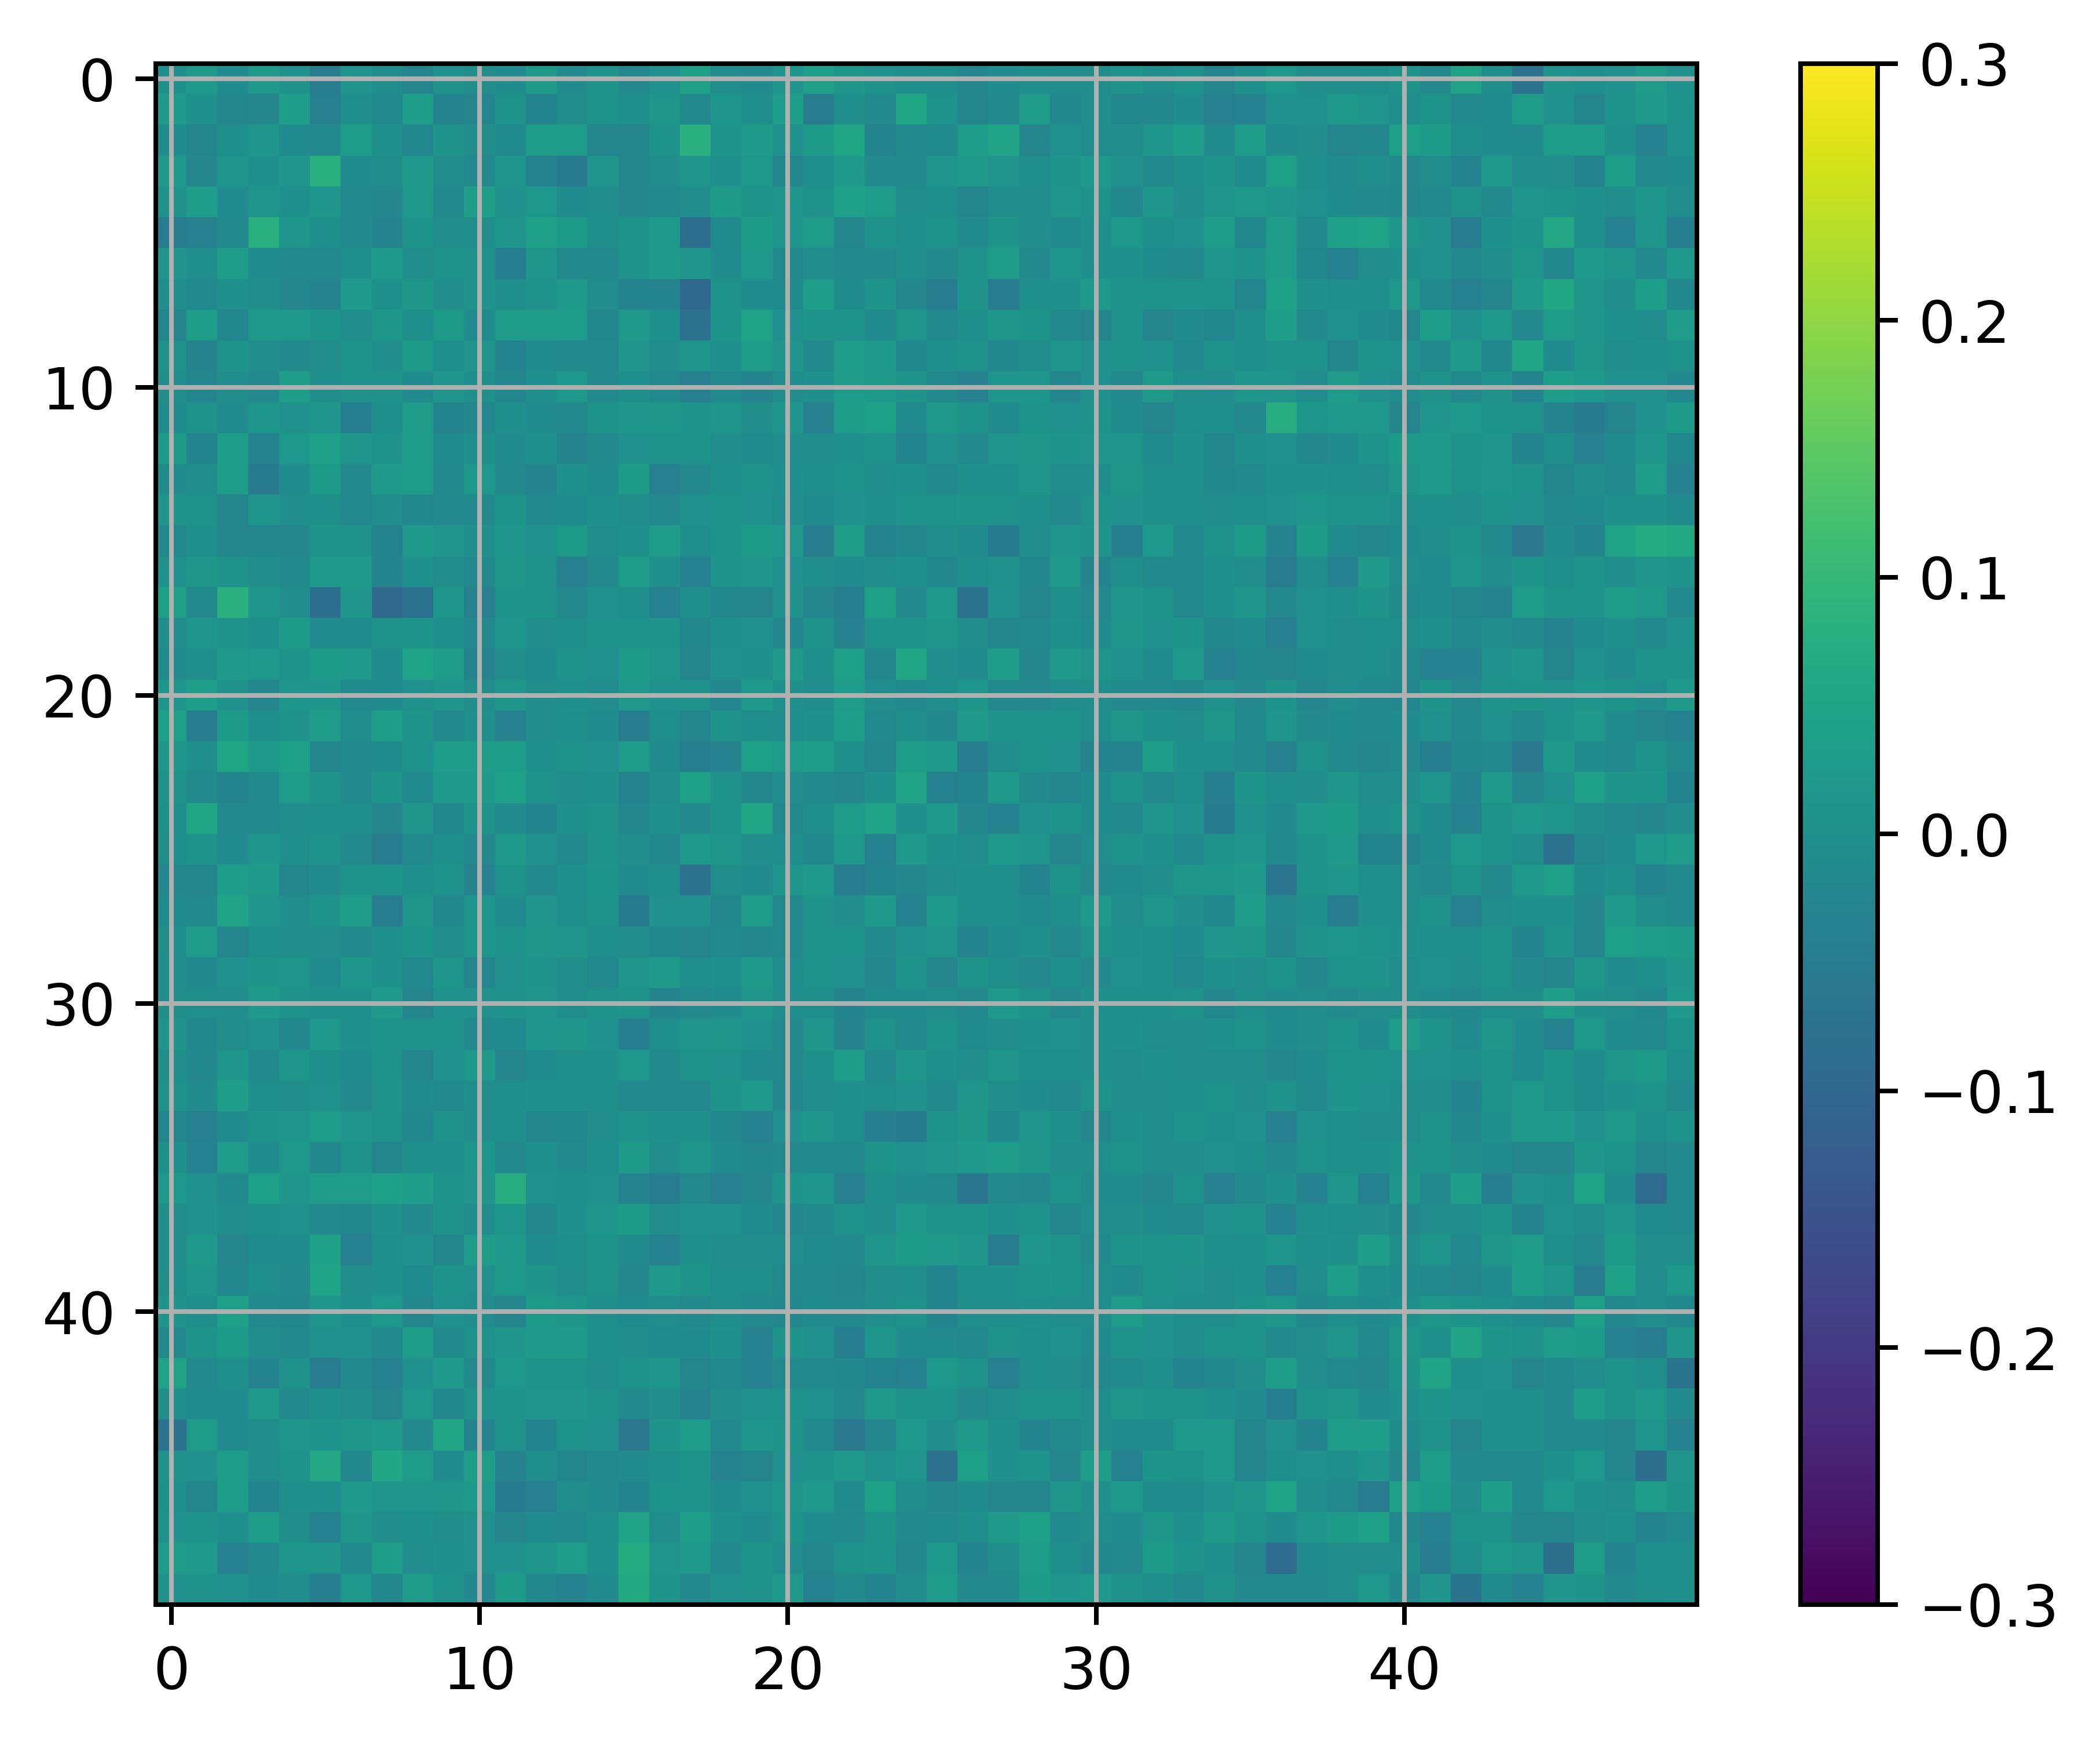
\includegraphics[width=0.2\textwidth]{../Analysis/DFC/size=480_step=180_rho=0.1/node=50_id=100206/c_12.jpg}
        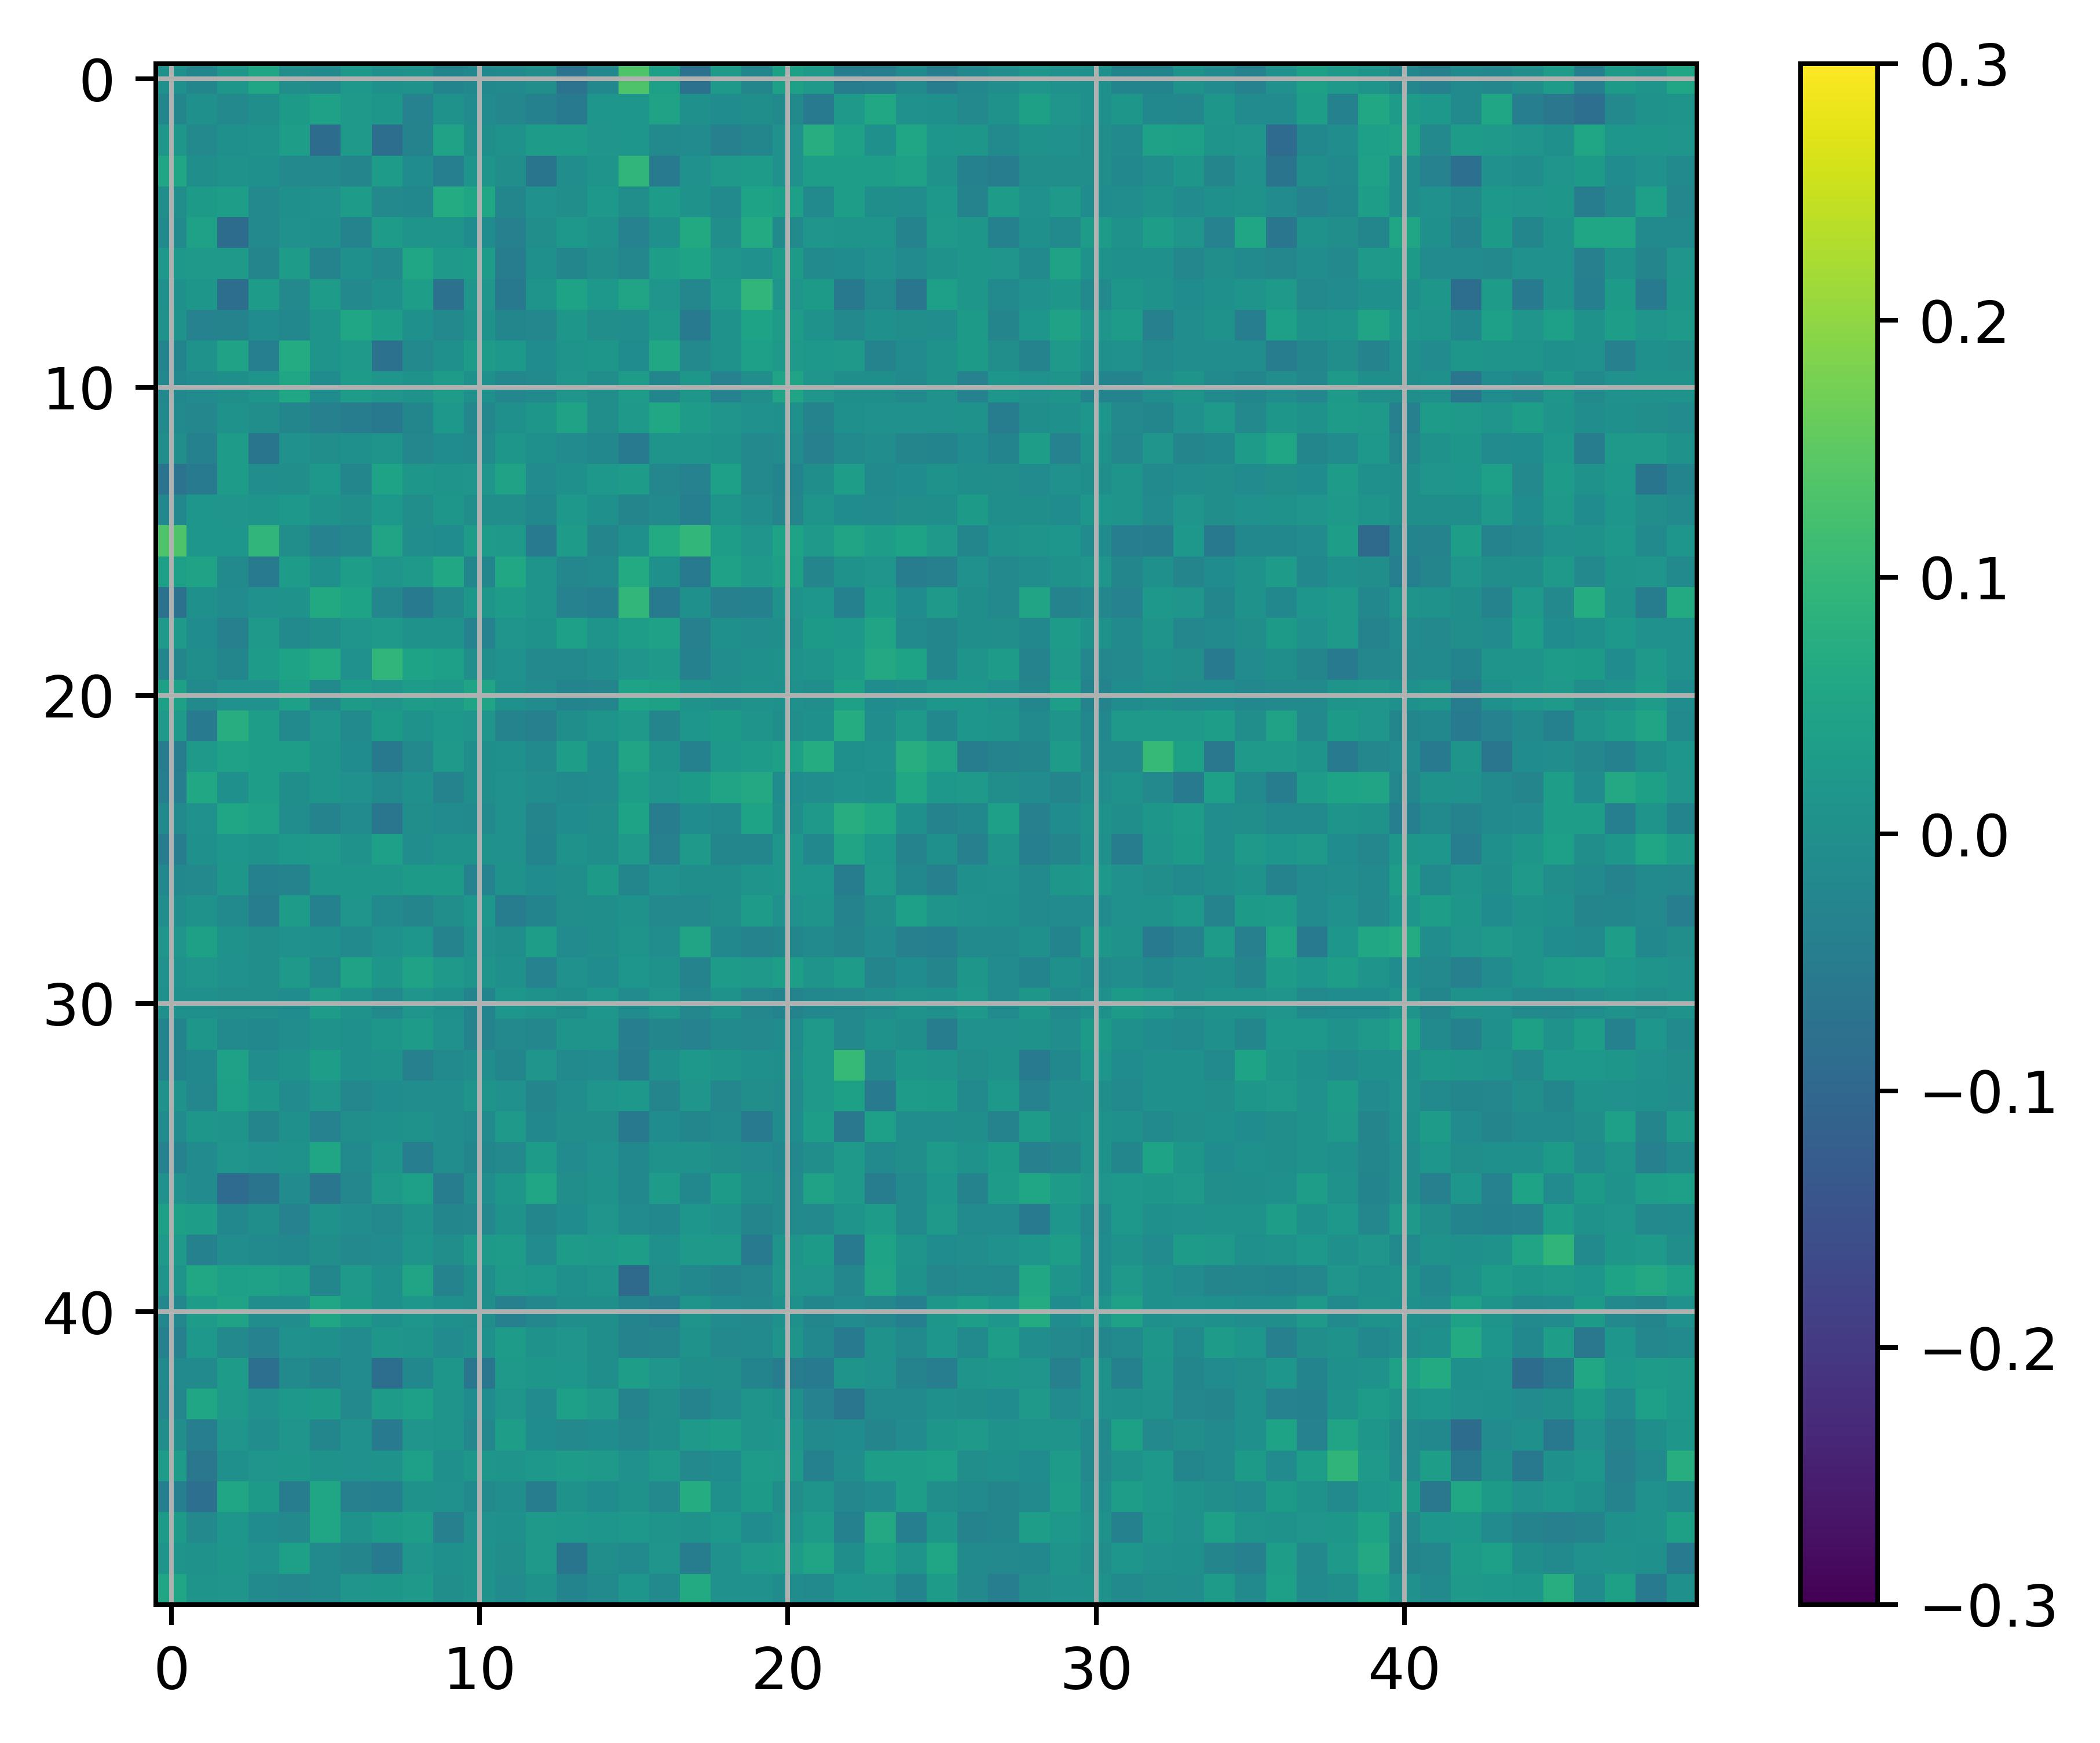
\includegraphics[width=0.2\textwidth]{../Analysis/DFC/size=480_step=180_rho=0.1/node=50_id=100206/c_14.jpg} \\
        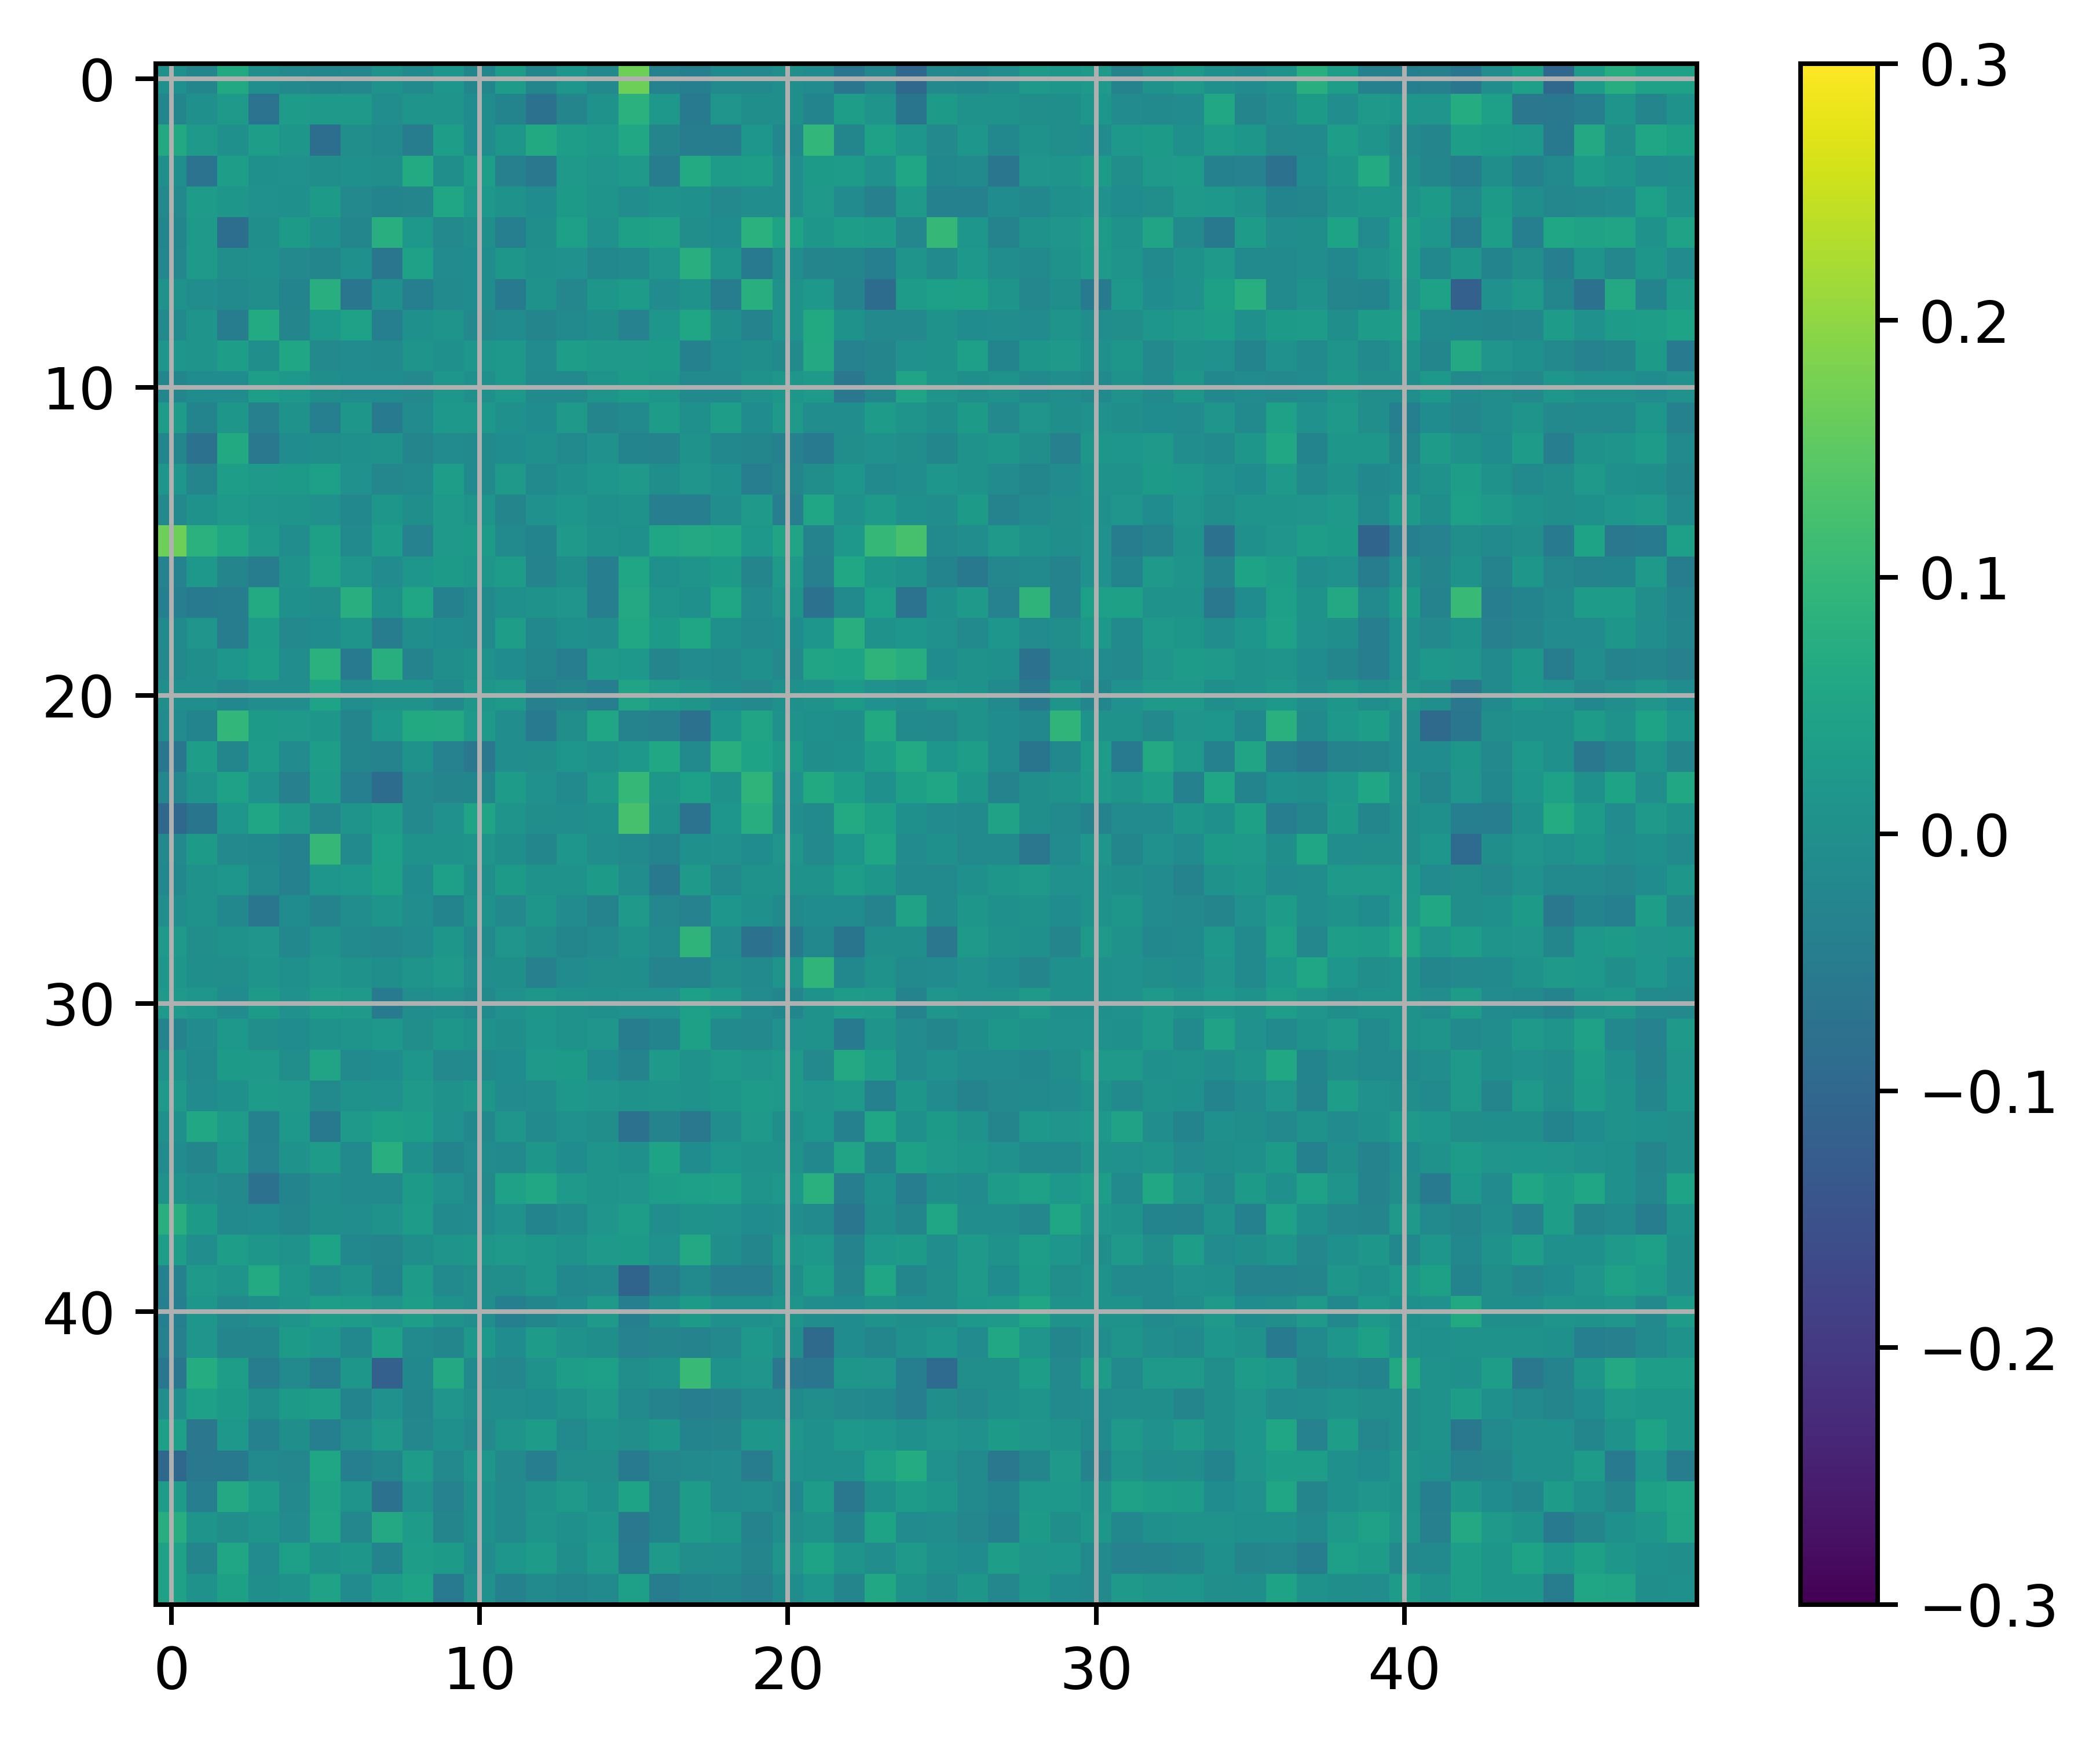
\includegraphics[width=0.2\textwidth]{../Analysis/DFC/size=480_step=180_rho=0.1/node=50_id=100206/c_16.jpg}
        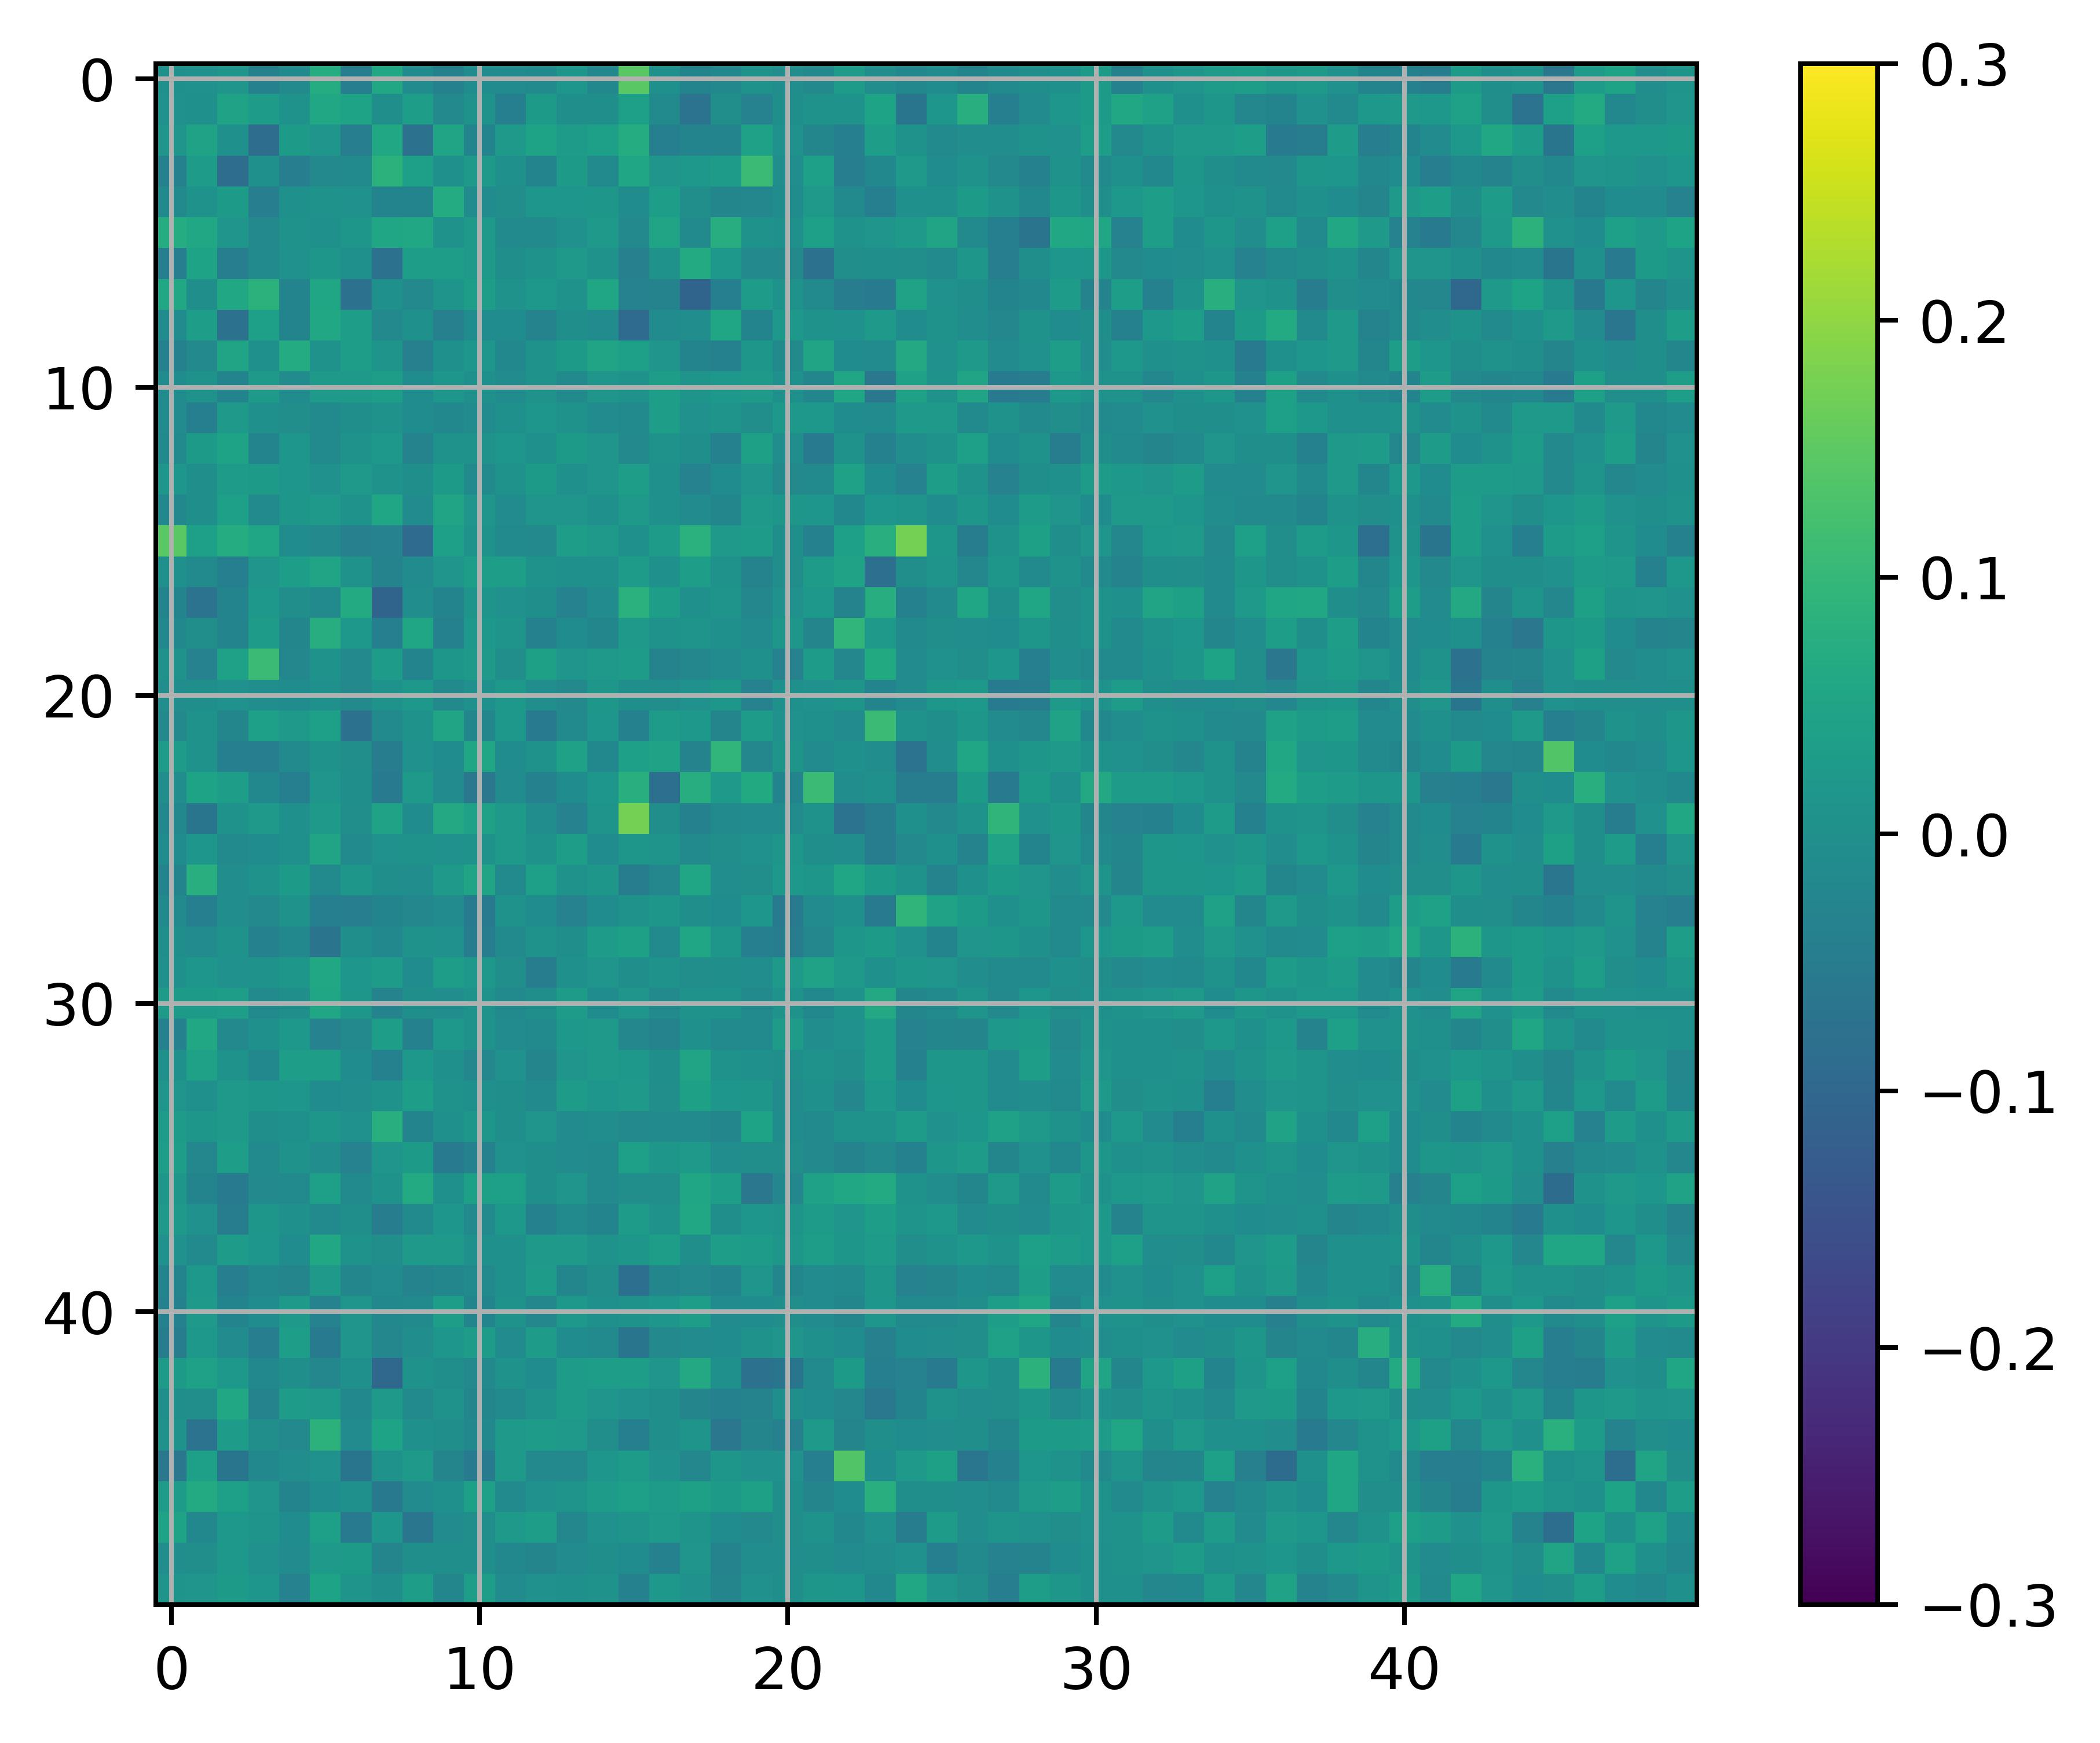
\includegraphics[width=0.2\textwidth]{../Analysis/DFC/size=480_step=180_rho=0.1/node=50_id=100206/c_18.jpg}
        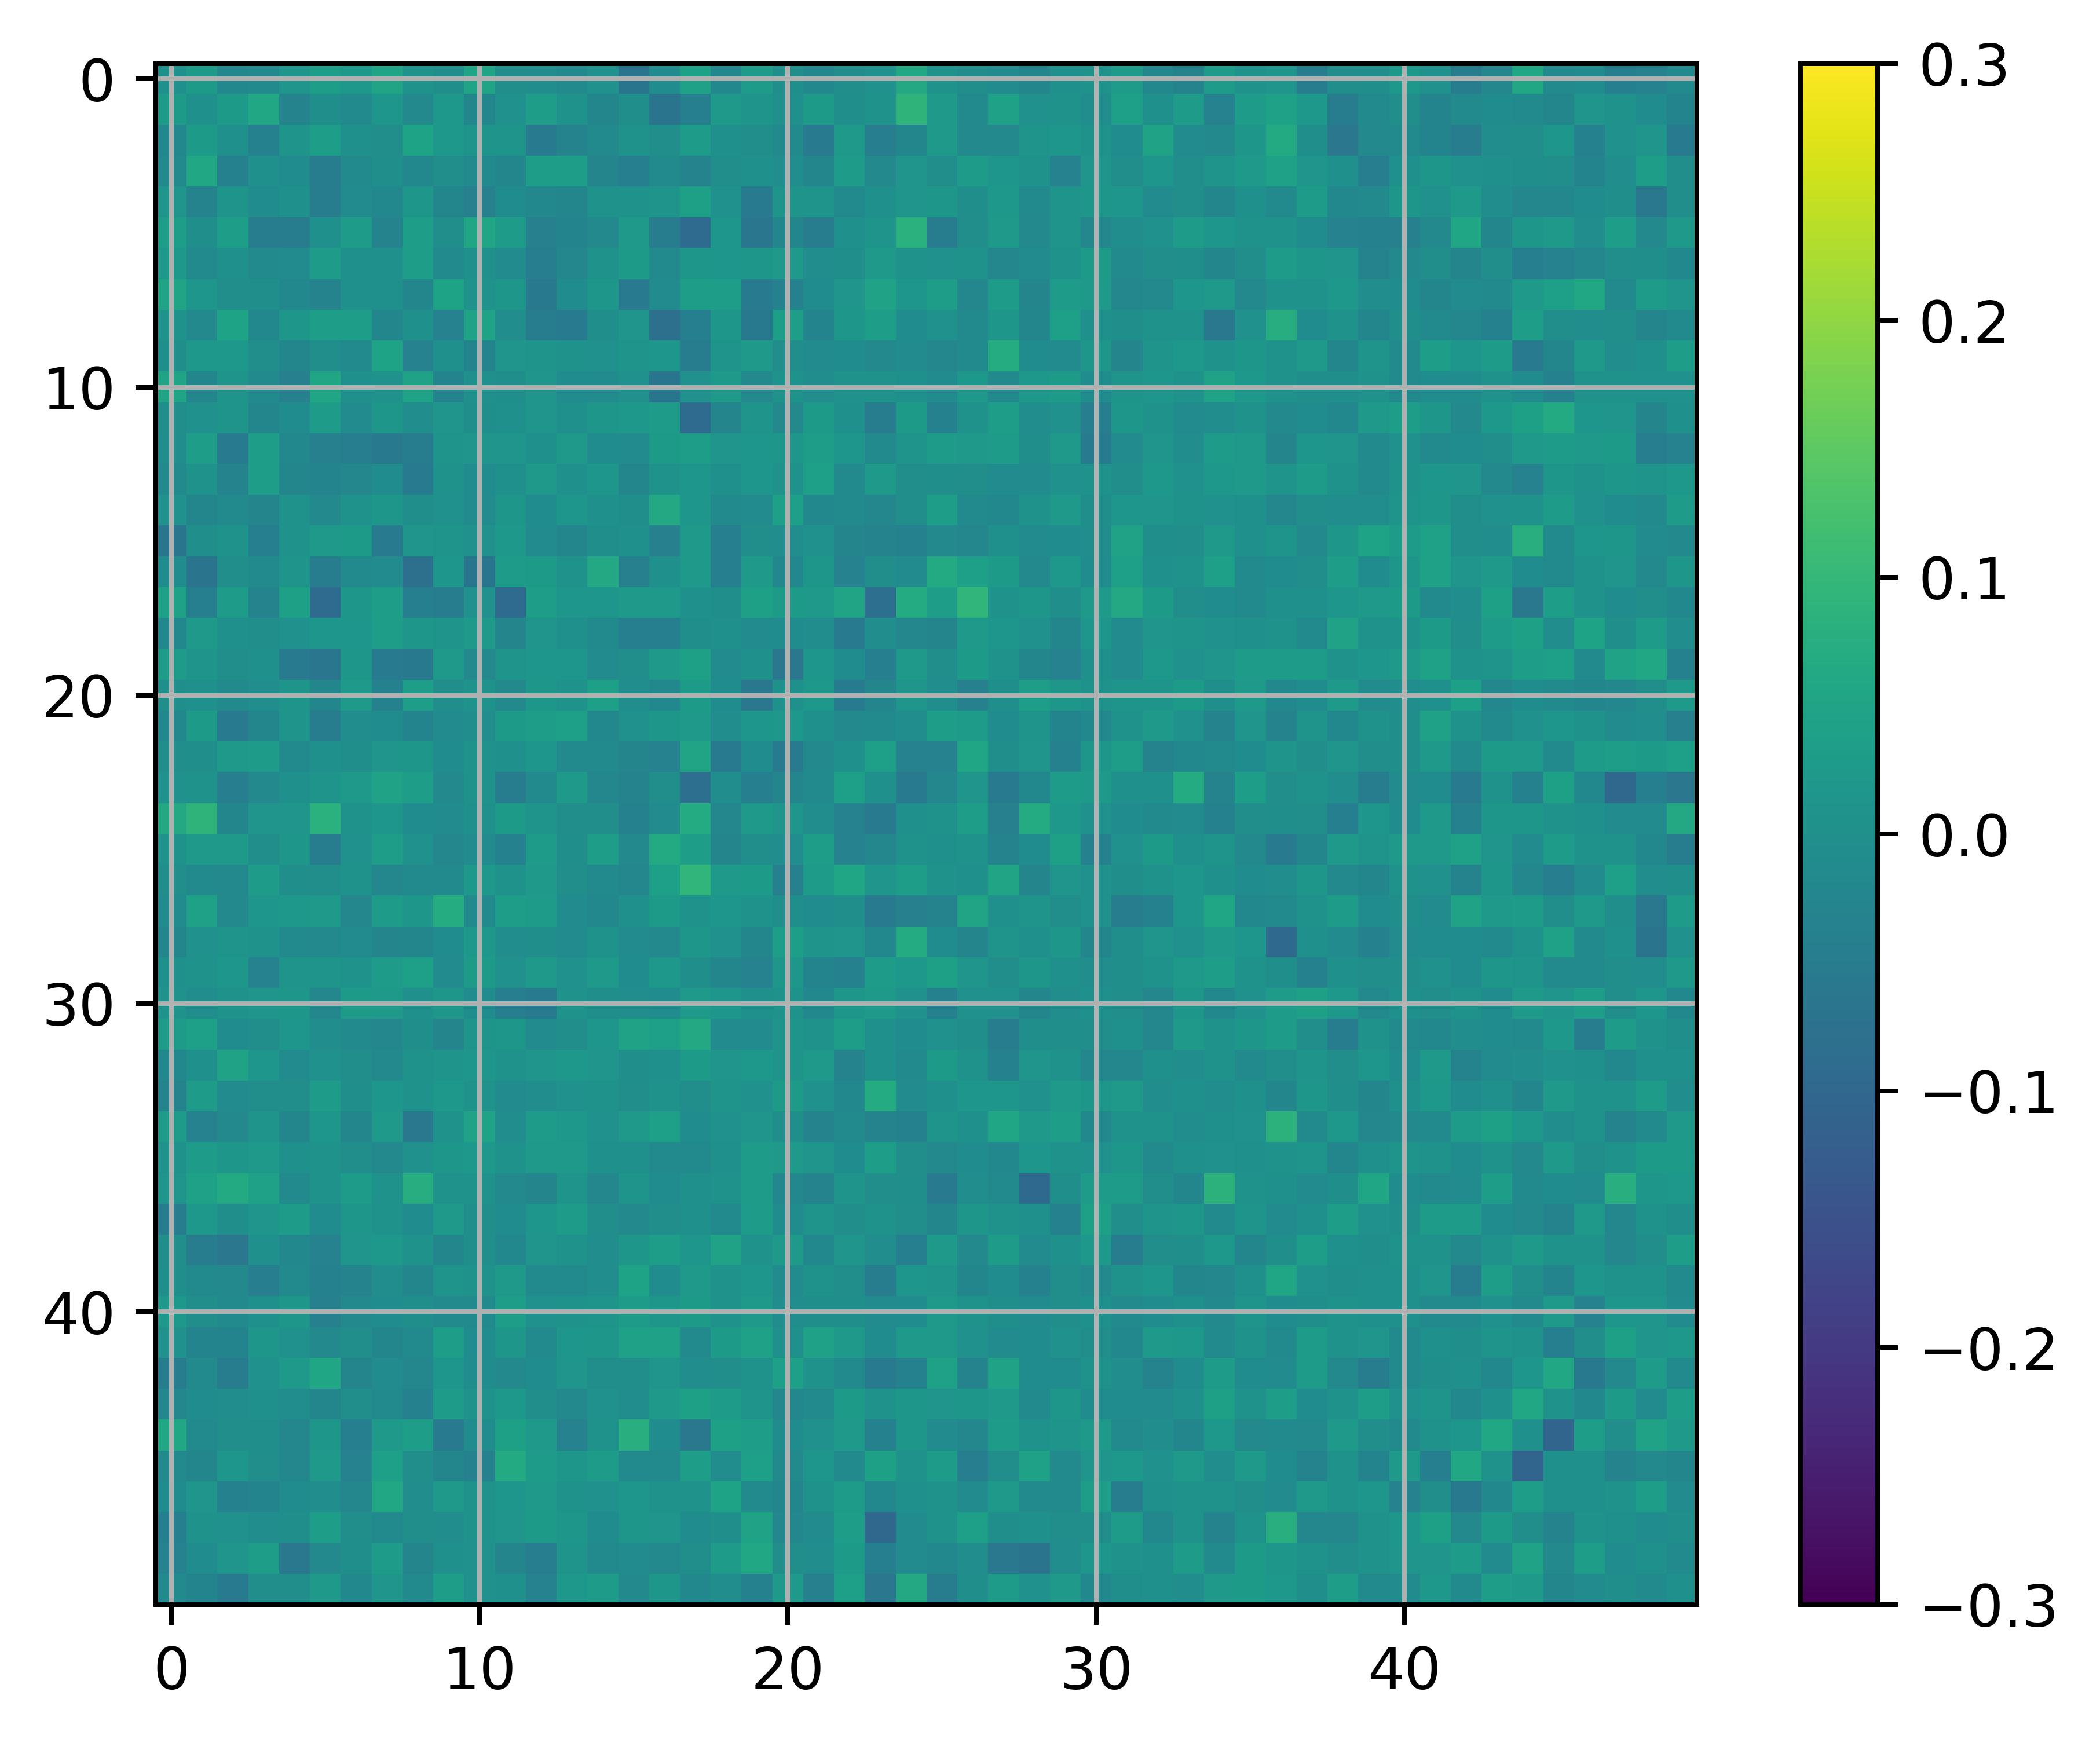
\includegraphics[width=0.2\textwidth]{../Analysis/DFC/size=480_step=180_rho=0.1/node=50_id=100206/c_20.jpg}
        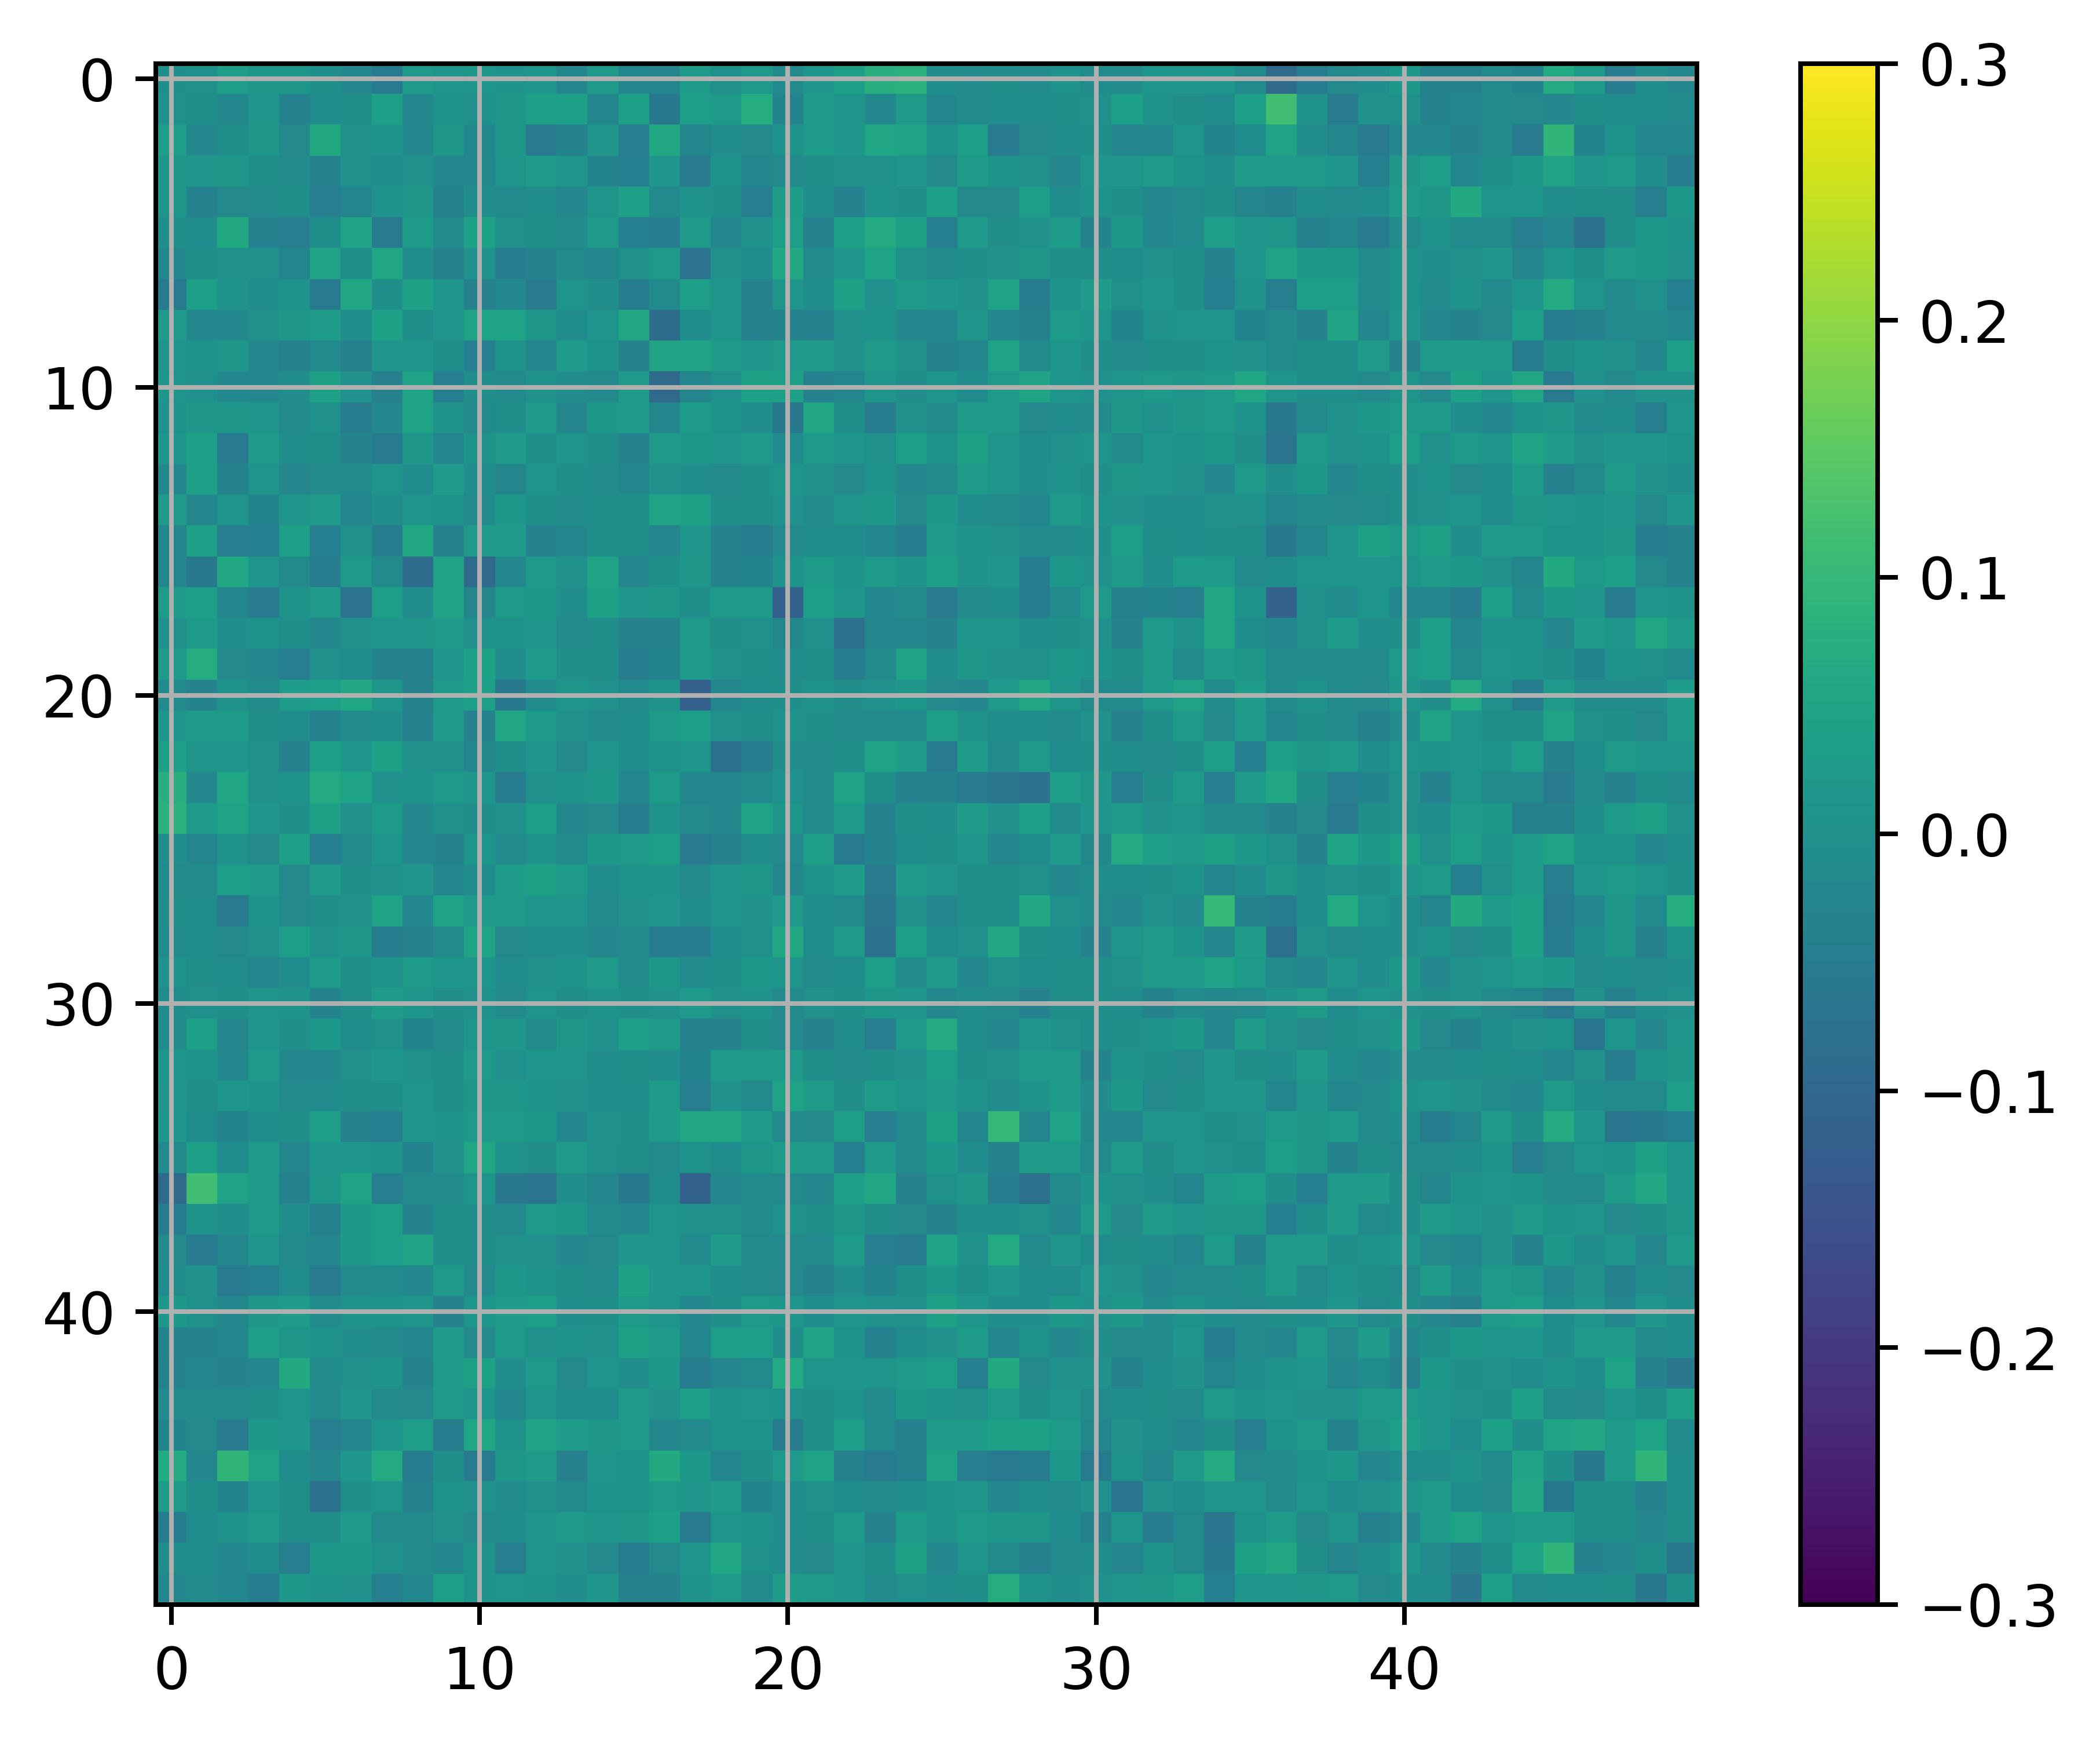
\includegraphics[width=0.2\textwidth]{../Analysis/DFC/size=480_step=180_rho=0.1/node=50_id=100206/c_22.jpg} \\
        \caption{Centered dynamic functional connectivity with $N_{node} = 50$.}
        % \label{LDA-example-1}
    \end{figure}

\end{frame}

\begin{frame}{Preprocessing - Examples}

    We compute the variance of each entry in dFC, which shows that the frames of dFC are more uniform with the increase of node.

    \begin{table}[H]
        \centering
        \begin{tabular}{|c|c|c|c|}
            \hline
            $N_{node}$ & min     & mean    & max     \\
            \hline
            $15$       & 5.76e-6 & 2.80e-5 & 1.99e-4 \\
            \hline
            $25$       & 2.82e-6 & 1.07e-5 & 6.07e-5 \\
            \hline
            $50$       & 1.63e-8 & 1.34e-6 & 4.90e-6 \\
            \hline
        \end{tabular}
        % \label{table1}
        \caption{Variance of dFC}
    \end{table}

\end{frame}

% \begin{frame}{Method}

%     With a fixed number of training samples, the predictive power reduces as the number of predictor variables increases\footfullcite{Hughes1968-ga}.

% \end{frame}

\begin{frame}{SVM\footfullcite{Vapnik1997-yy}\footfullcite{Cortes1995-dg}}

    Given a dataset $\{ (\mathbf{x}_i, y_i) \}_{i=1}^N$, a linear SVM aims to find a vector $\mathbf{w}$ and a number $b$ such that the data can be separated via the distance $\mathbf{w}^T \mathbf{x}_i - b$.

    \begin{figure}[H]
        \centering
        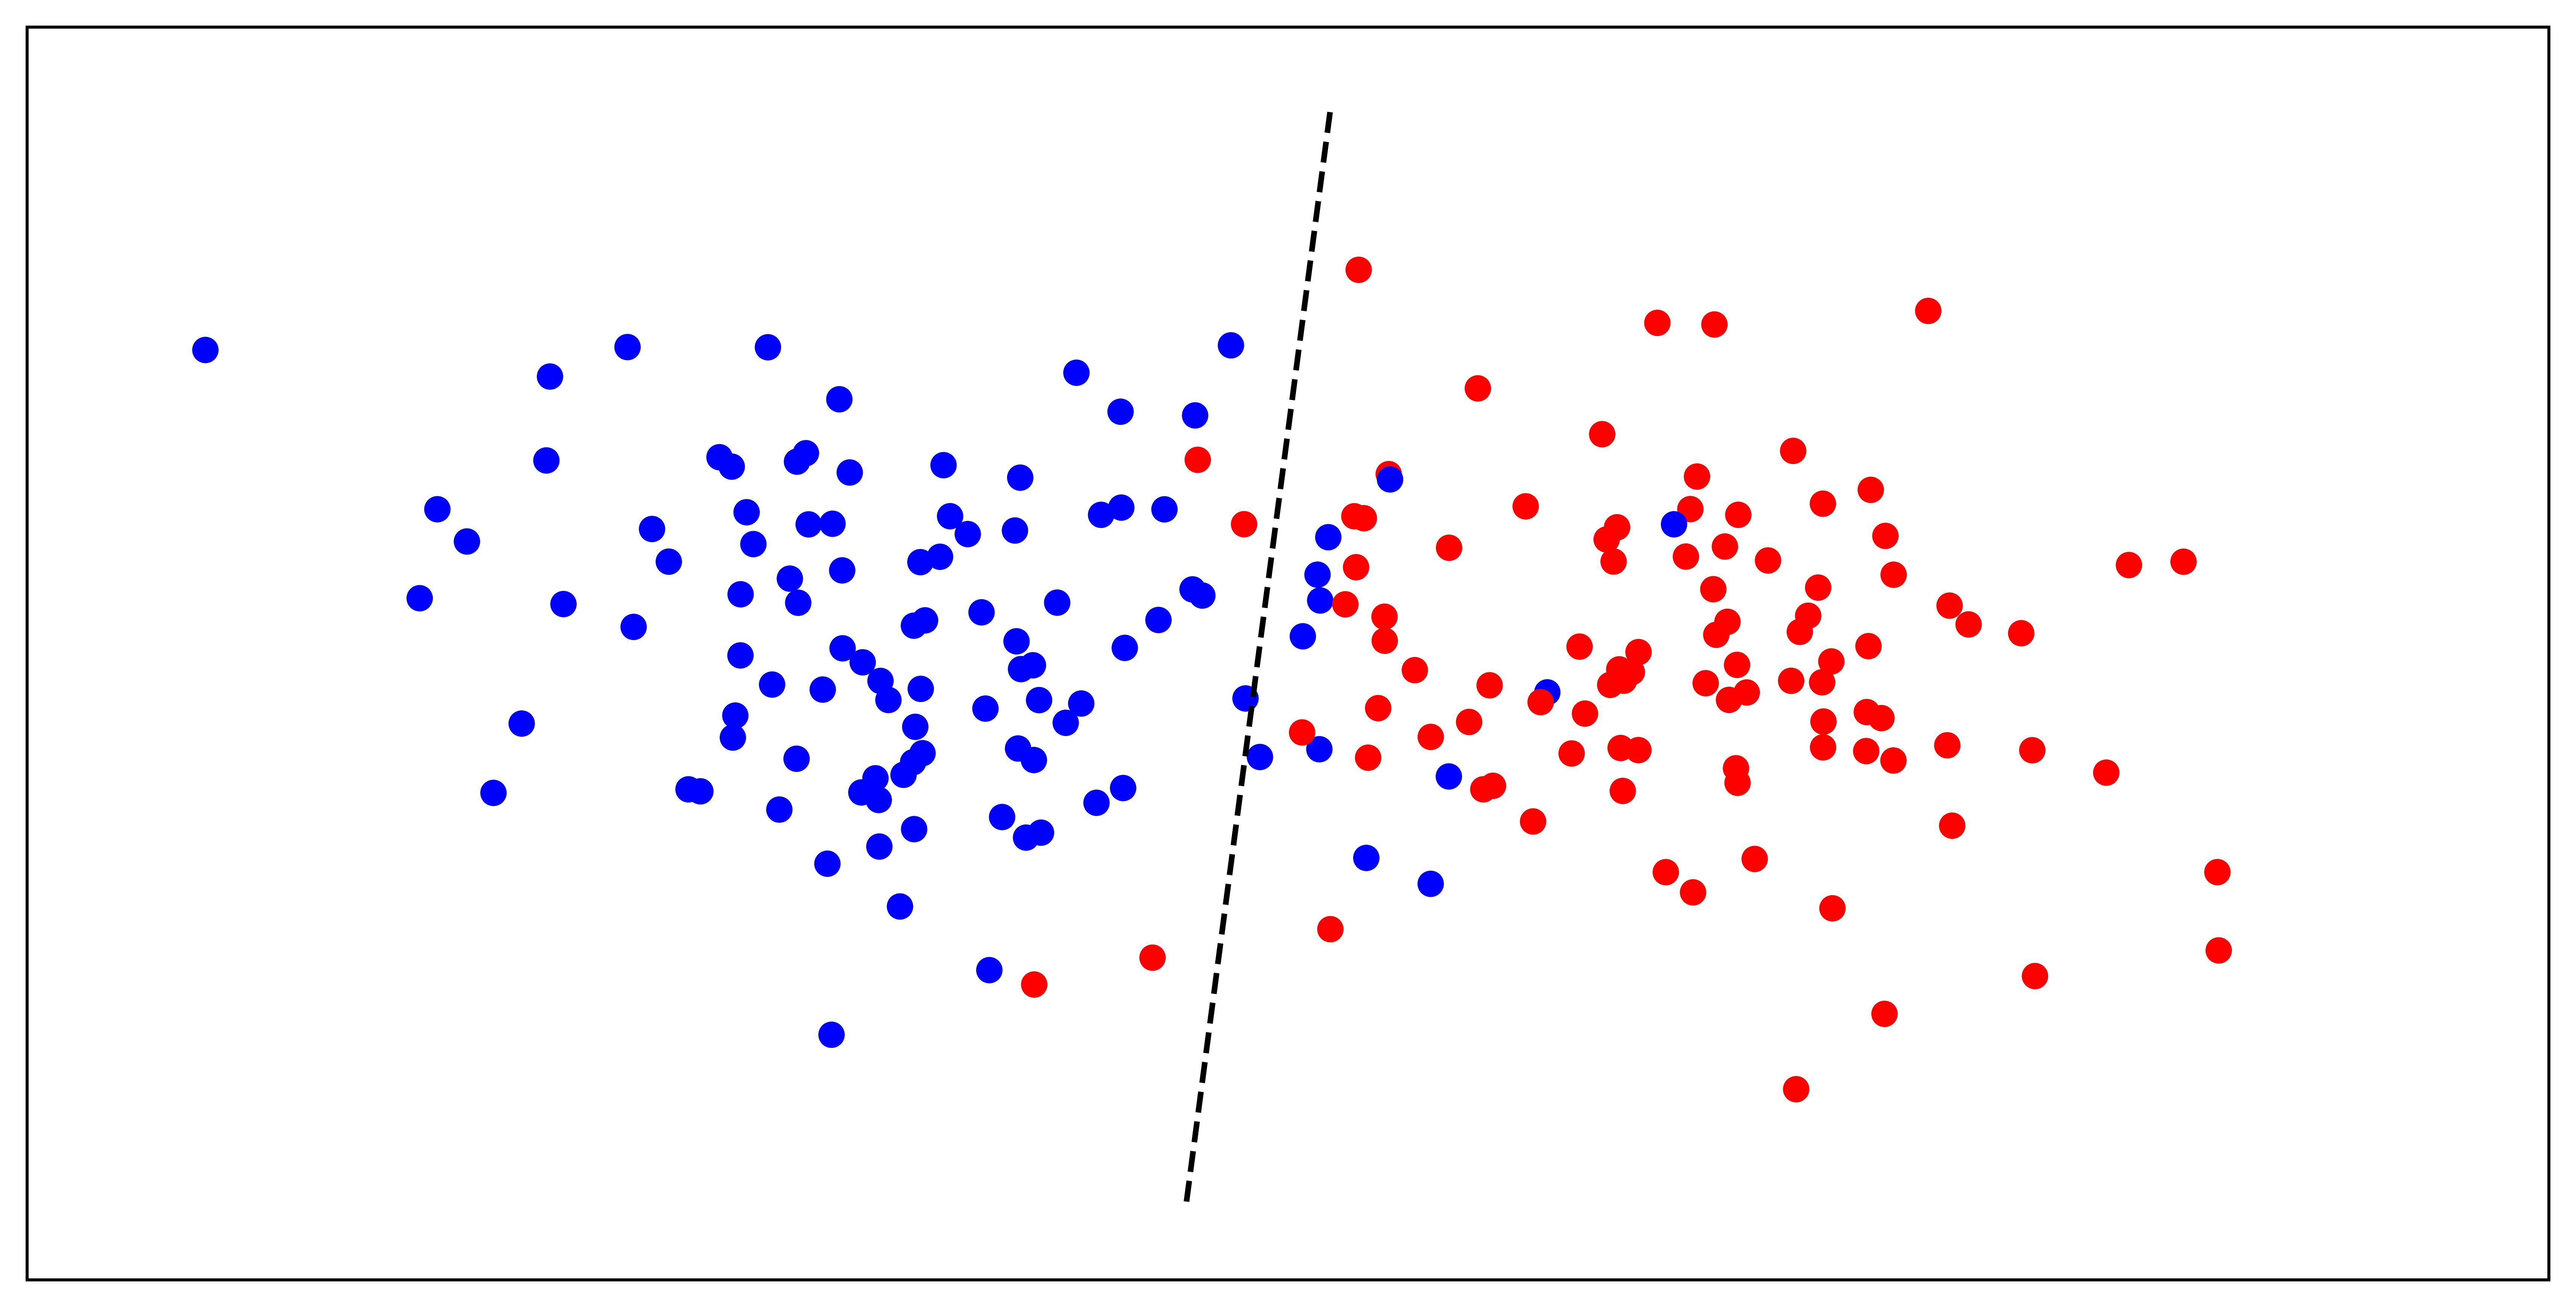
\includegraphics[width=0.6\textwidth]{./figure/svm.jpg}
    \end{figure}

\end{frame}

\begin{frame}{SVM - Results}

    \begin{figure}[H]
        \centering
        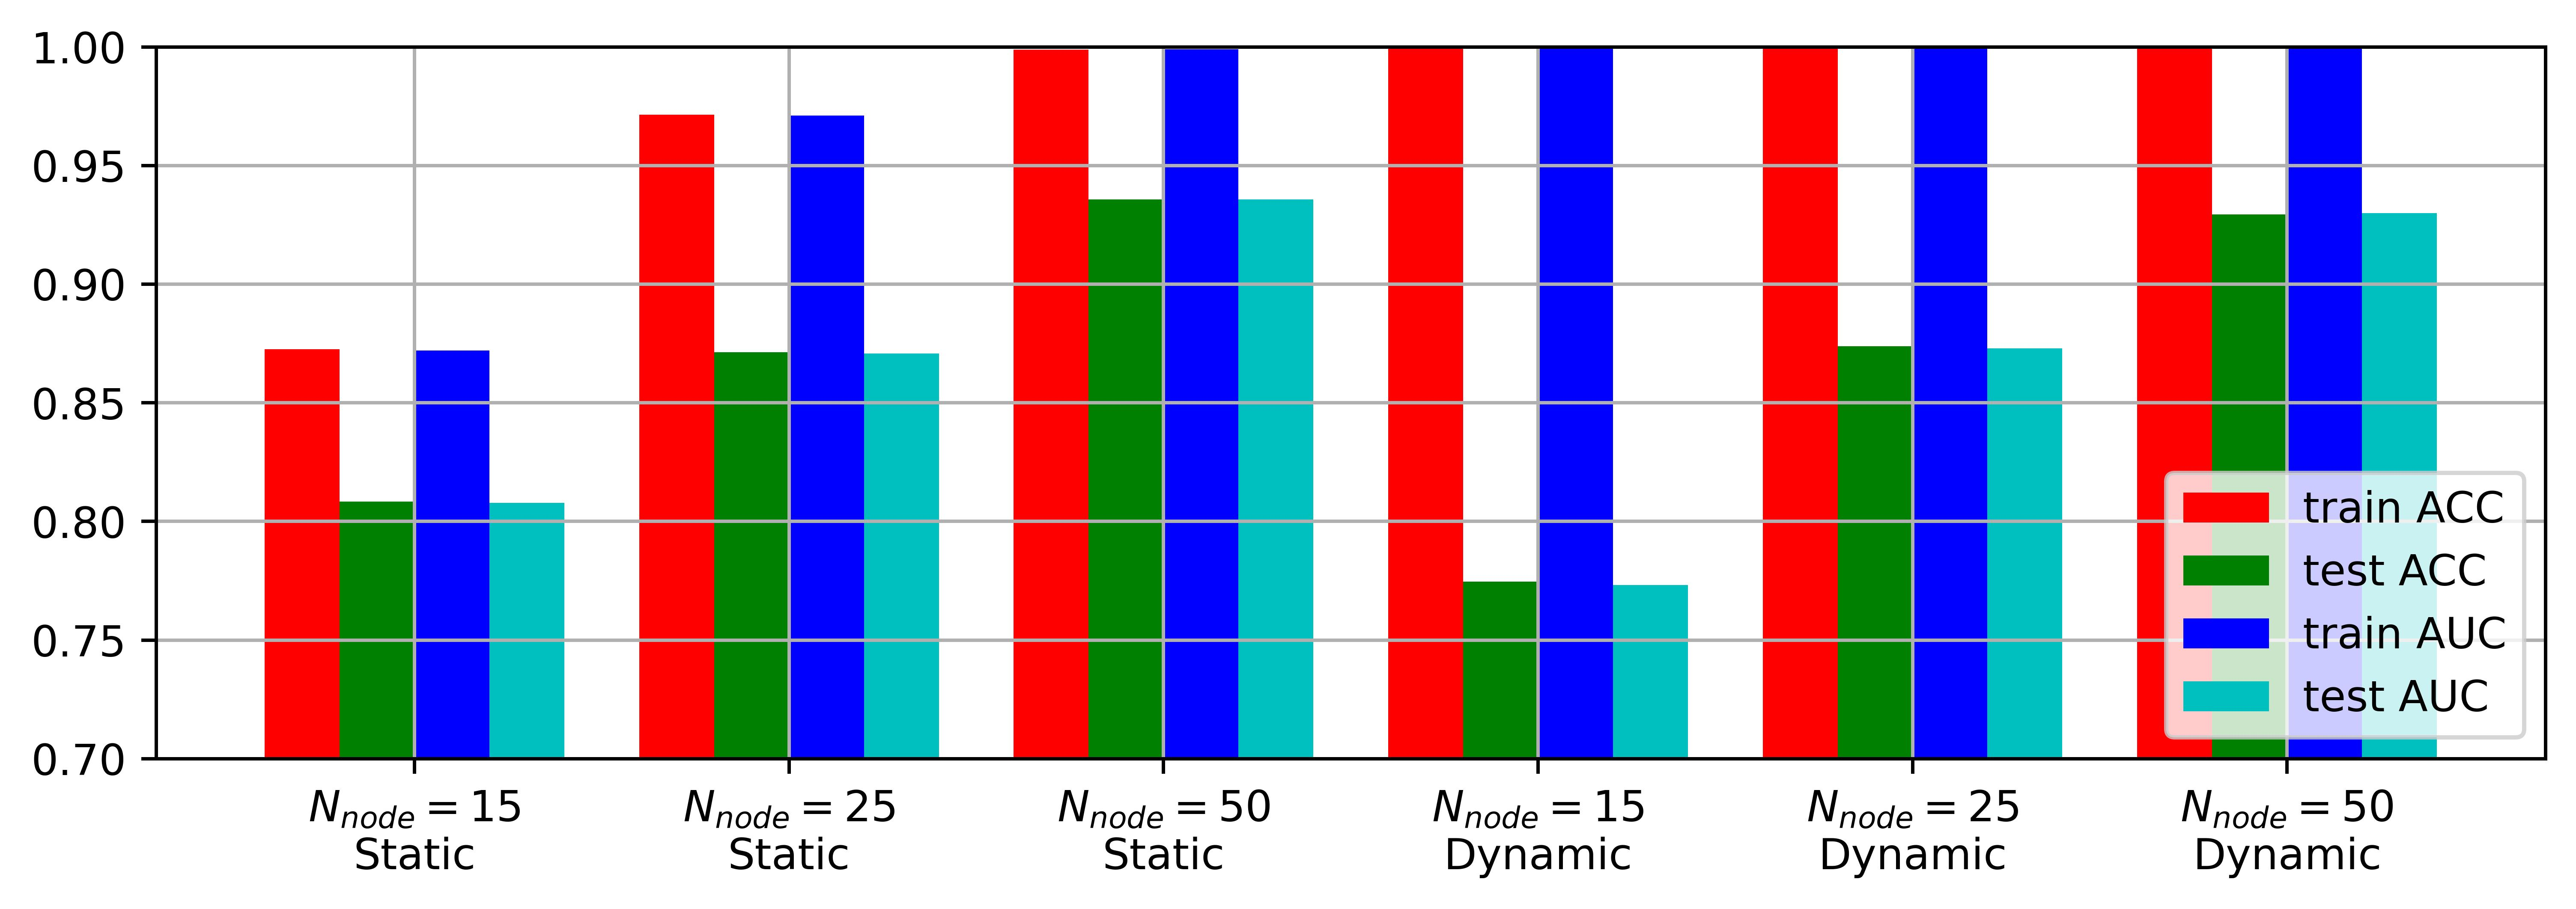
\includegraphics[width=0.6\textwidth]{../SVM/linear_0.1.jpg} \\
        \caption{Results of Linear SVM.}
    \end{figure}

    \begin{figure}[H]
        \centering
        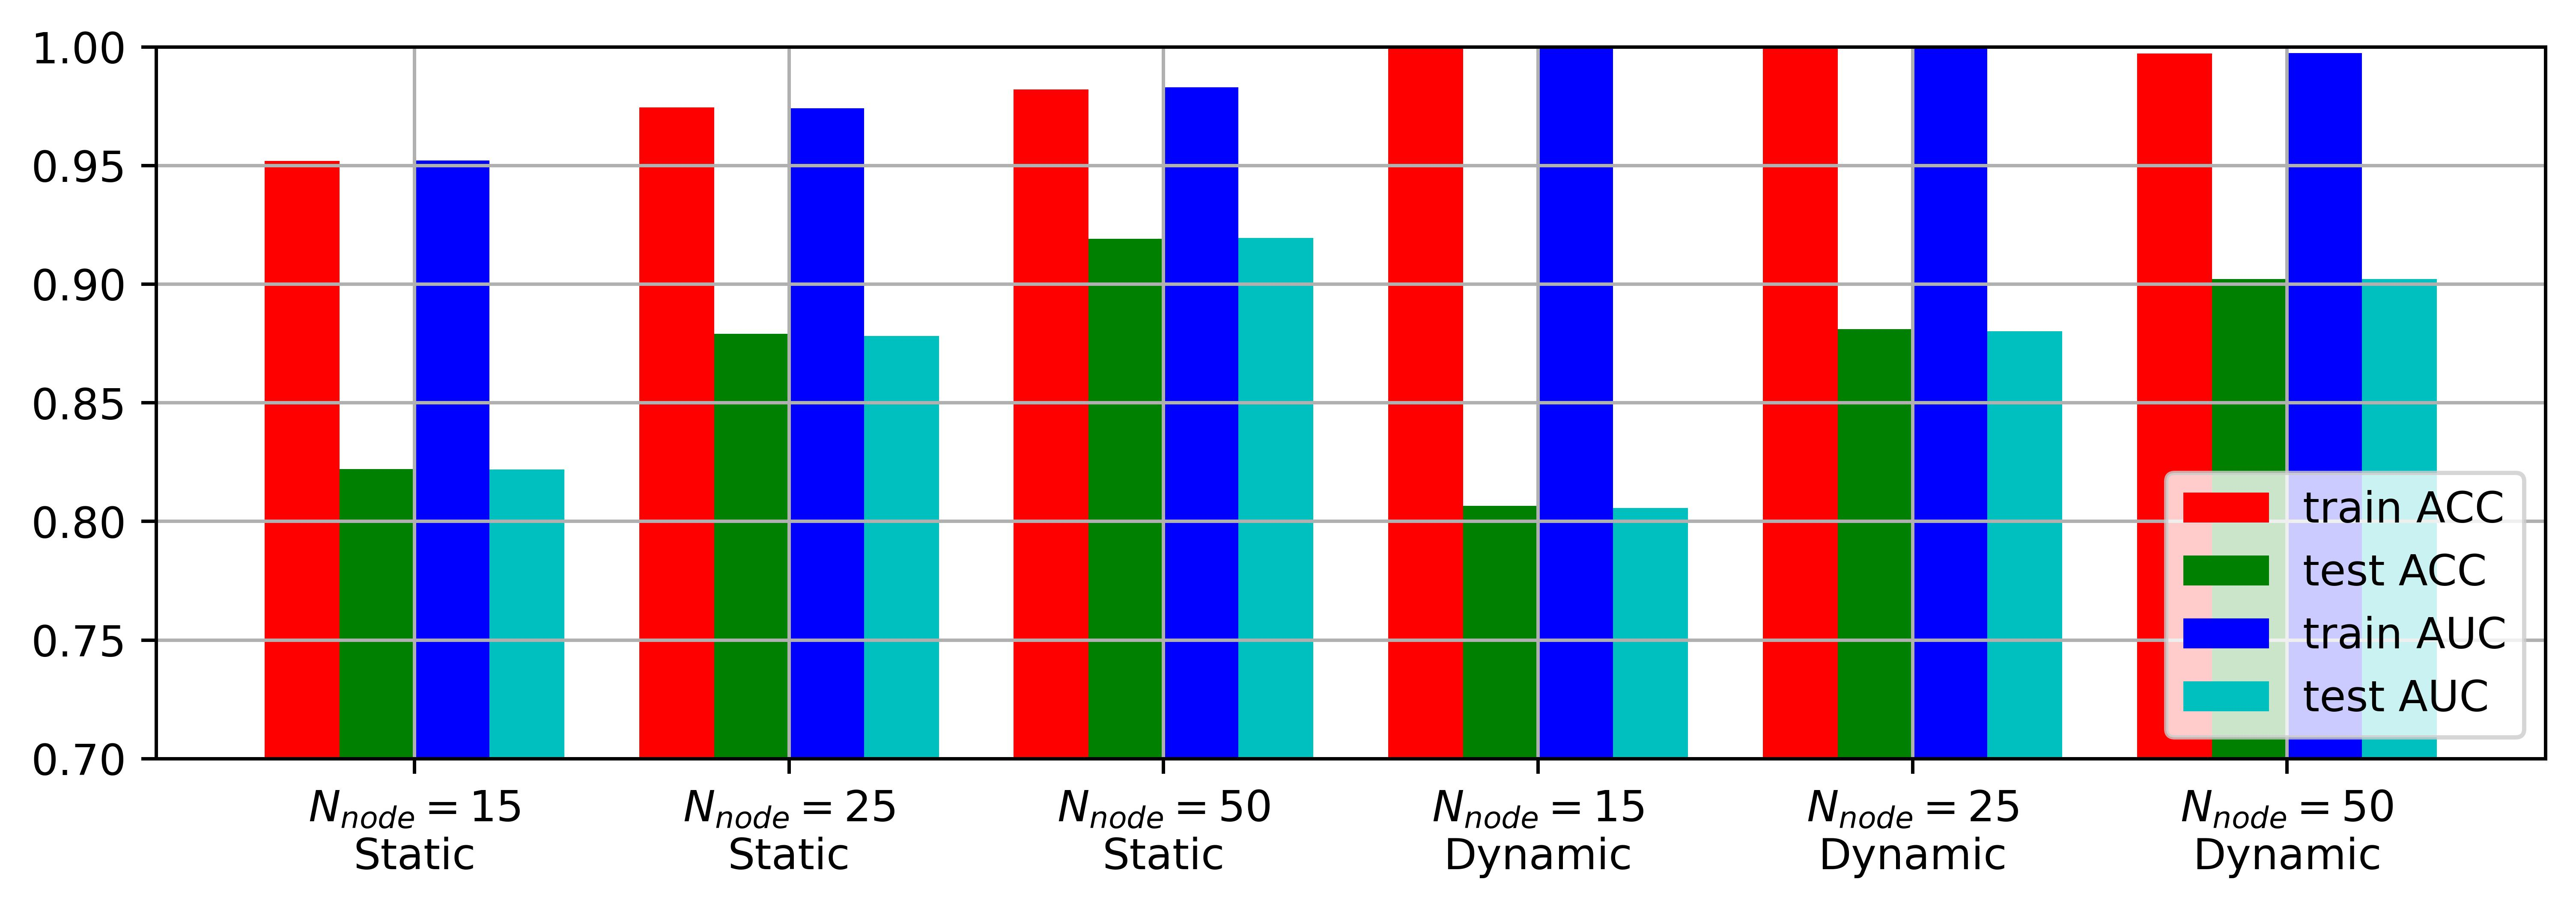
\includegraphics[width=0.6\textwidth]{../SVM/nu_0.1.jpg} \\
        \caption{Results of Nu-SVM.}
    \end{figure}

\end{frame}

\begin{frame}{CNN - Model}

    Given a dataset $\{ (\mathbf{x}_i, y_i) \}_{i=1}^N$, we aims to find some vectors $\{\mathbf{w}_k\}_{k=1}^m$ and some numbers $\{b_k\}_{k=1}^m$ such that any given data $\mathbf{x}$ can be classificated via the tuple of distance $( \mathbf{w}_1^T \mathbf{x} - b_1, \dots, \mathbf{w}_m^T \mathbf{x} - b_m )$.

    In the worst case, all the $\mathbf{w}_k$ and $b_k$ are the same, then the results should be the same with linear SVM.

    \begin{figure}[H]
        \centering
        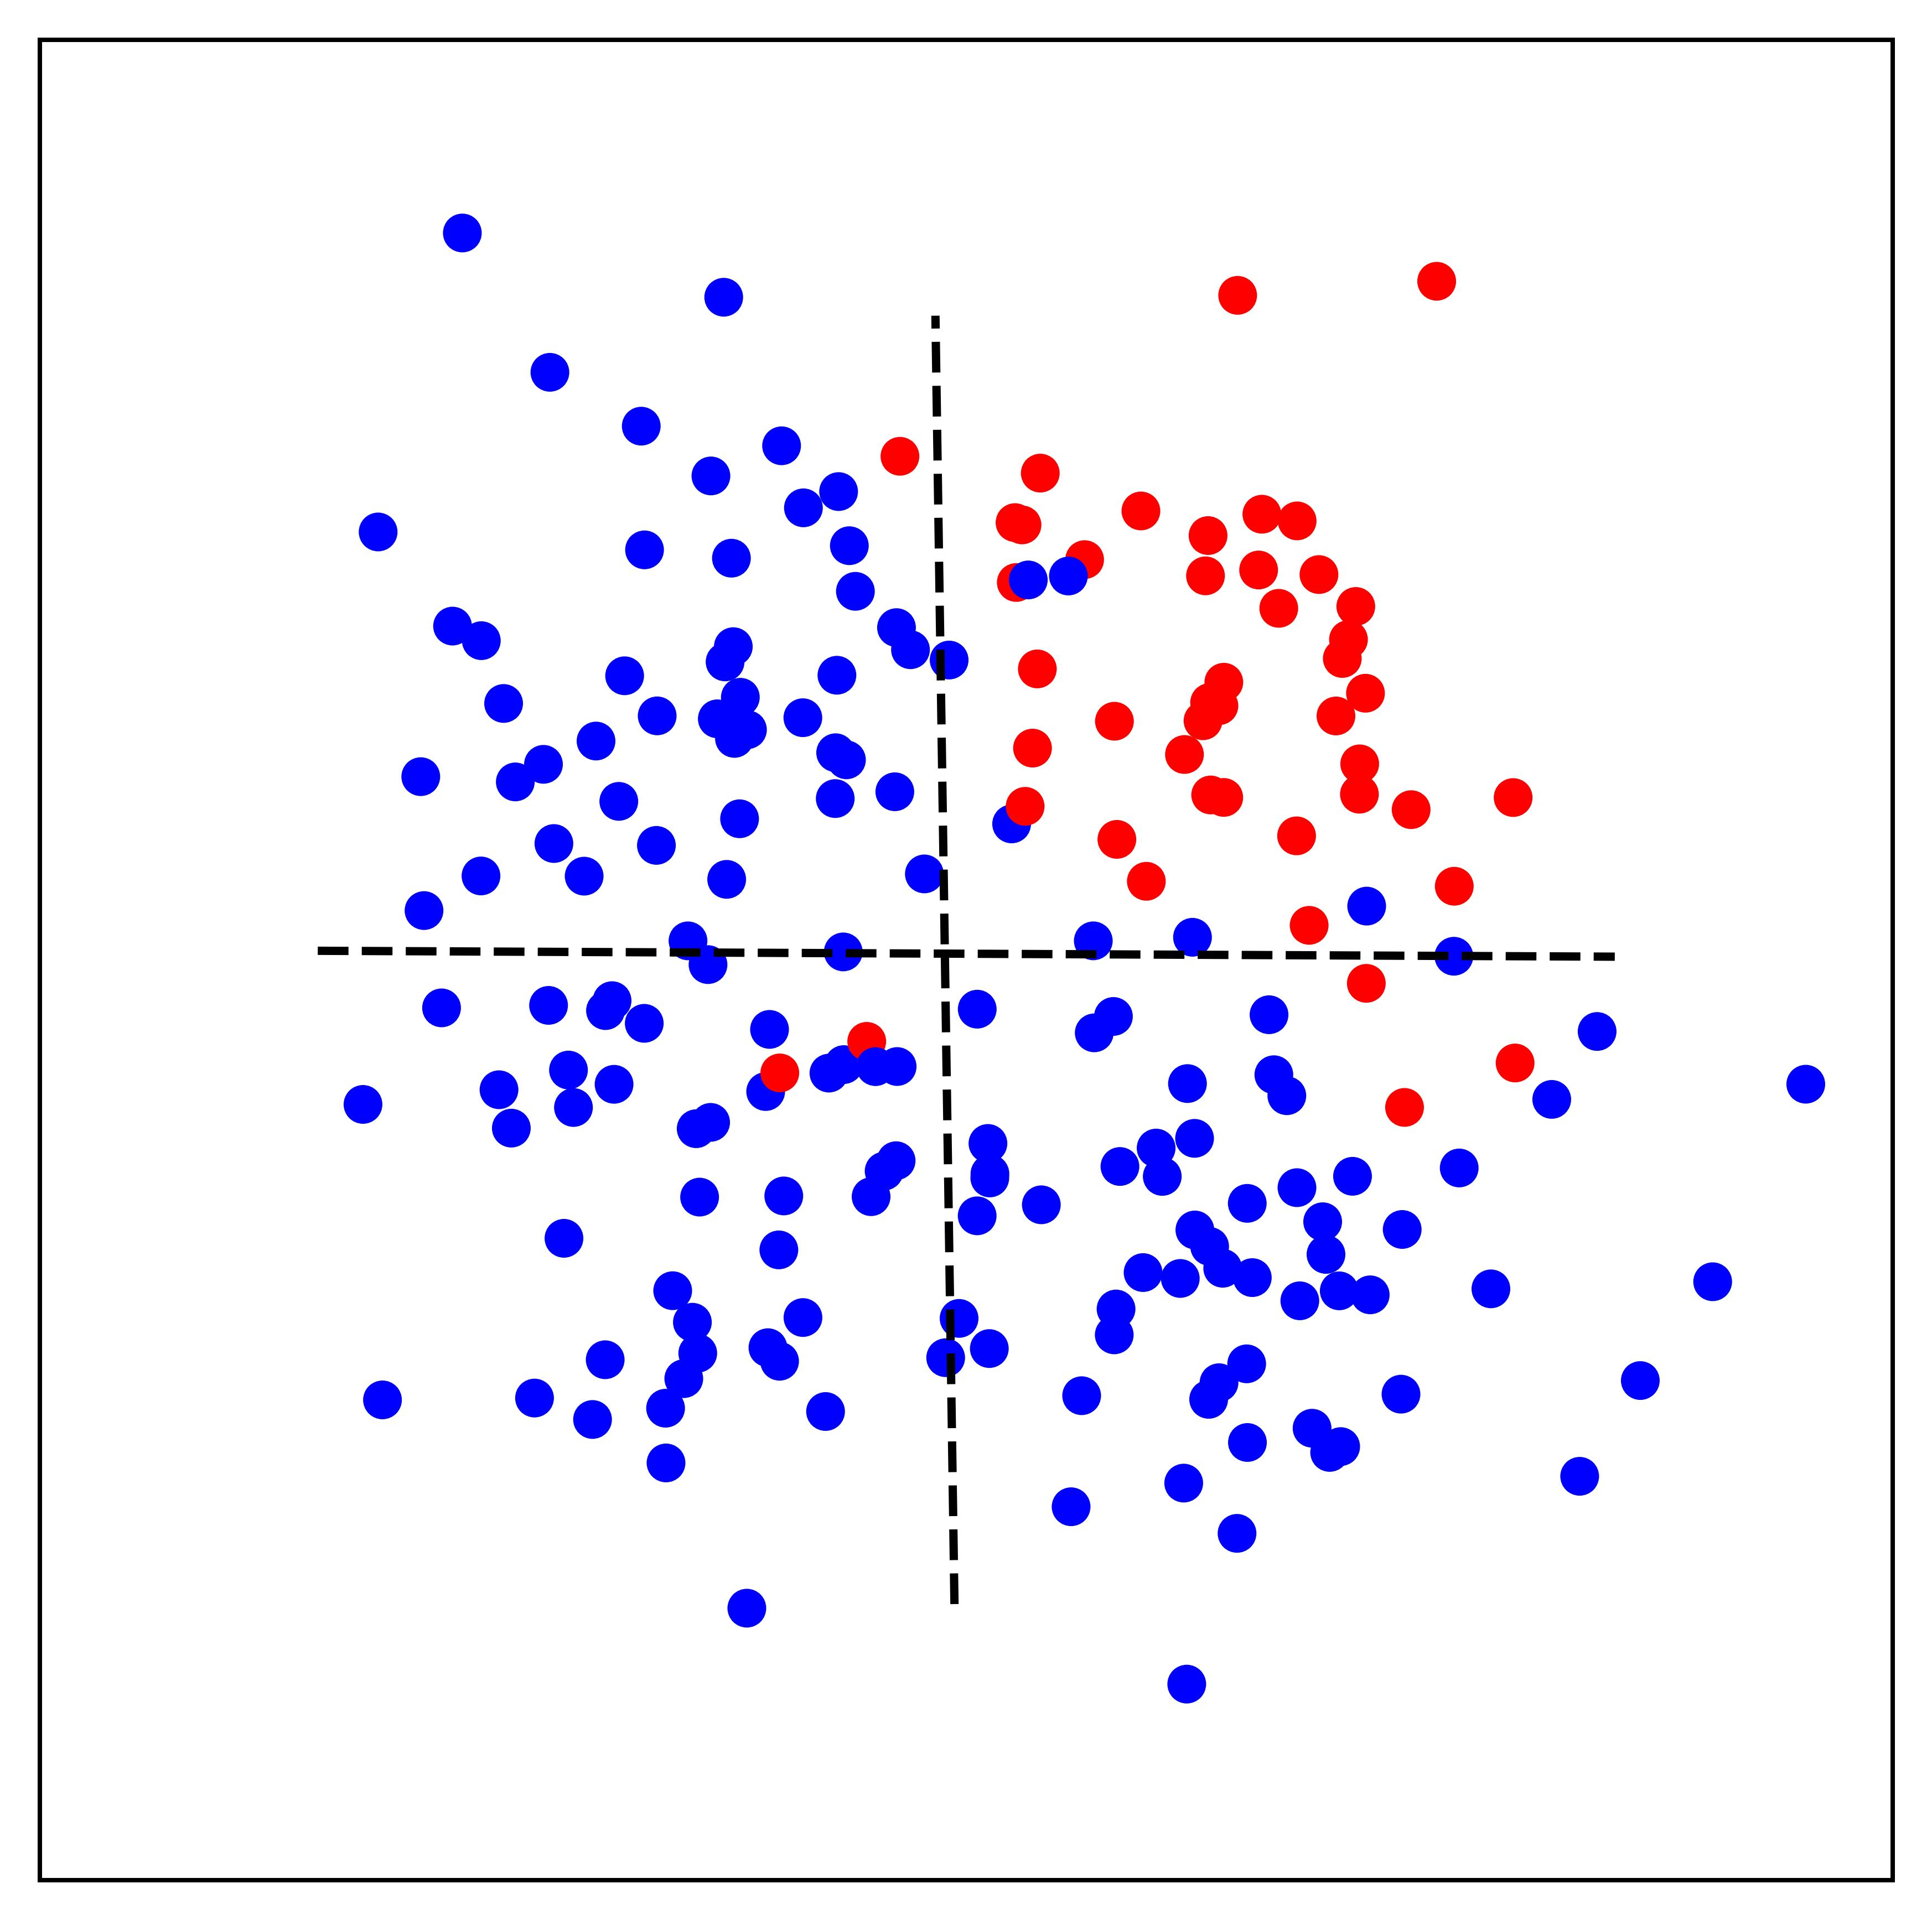
\includegraphics[width=0.3\textwidth]{./figure/model.jpg}
        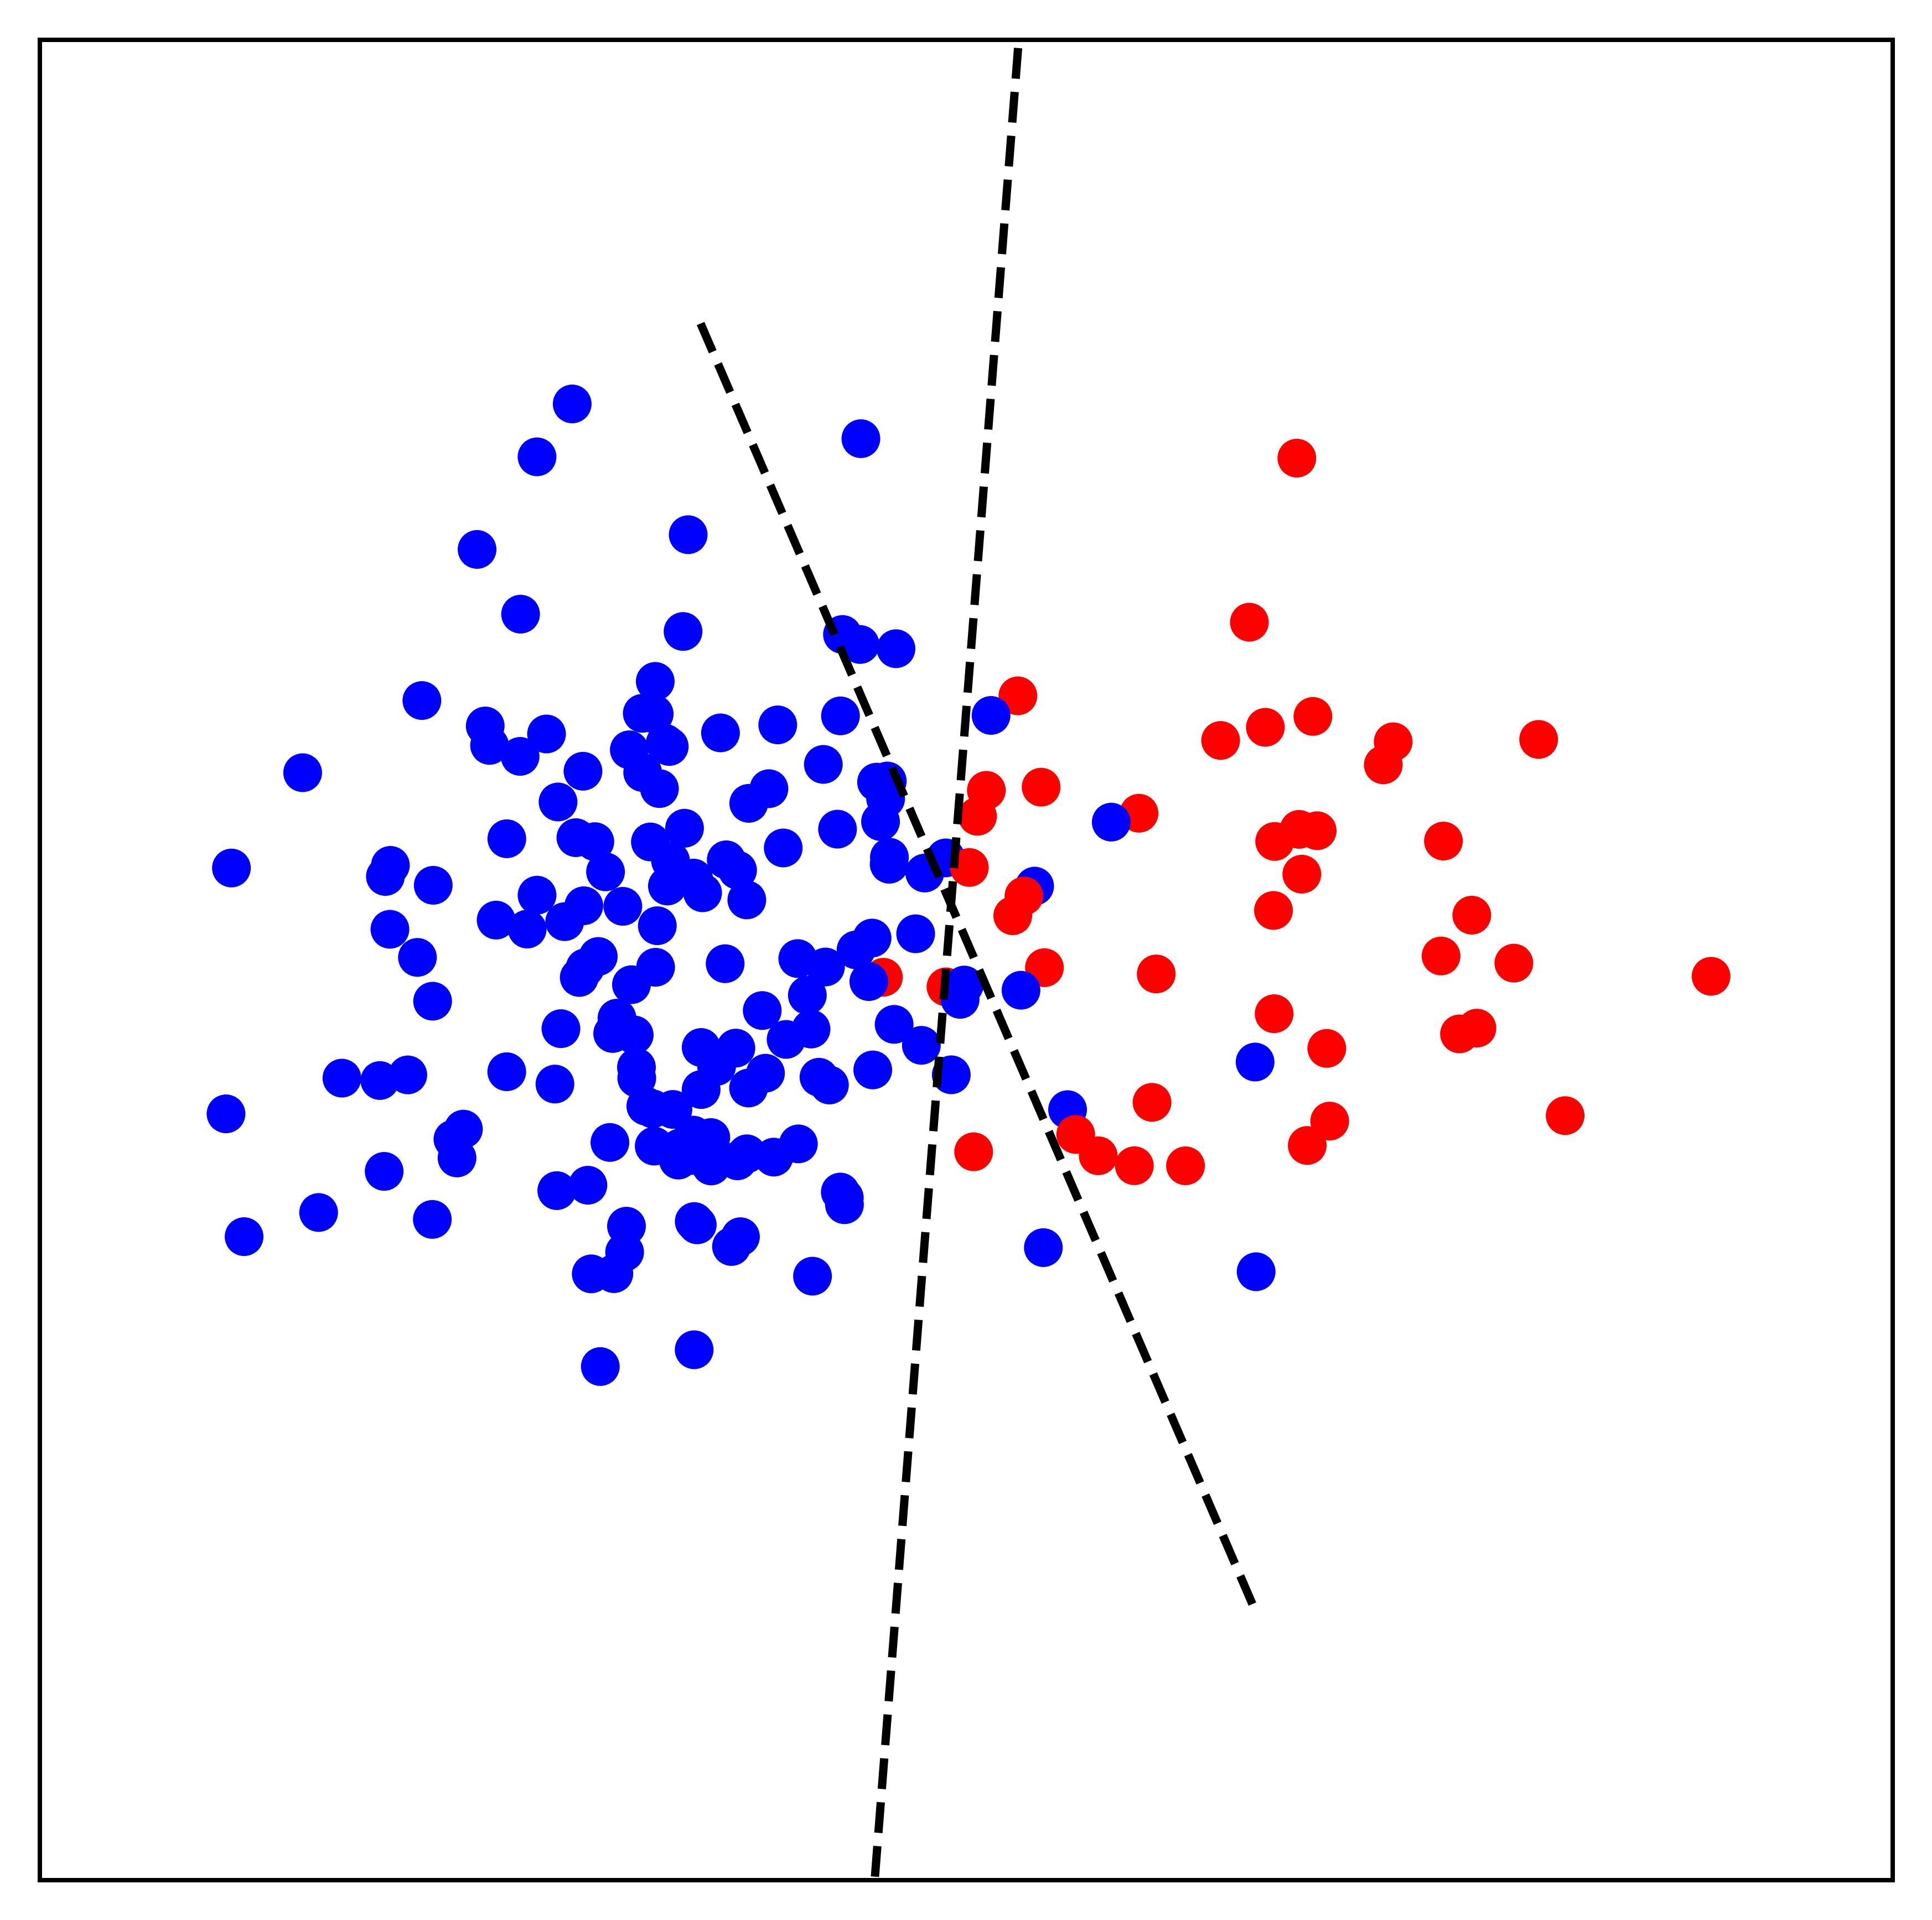
\includegraphics[width=0.3\textwidth]{./figure/model_worse.jpg}
    \end{figure}

\end{frame}

\begin{frame}{CNN - Model}

    The followings are the flowchart of our method, where we use a 1-layer 1-dimensional CNN with size equivalent to the input shape, so that it is the same as previous statements.

    \begin{figure}[H]
        \centering
        \includegraphics[width=0.8\textwidth]{./figure/method.png}
    \end{figure}

    We split the data into training dataset ($80\%$) and test dataset ($20\%$), and repeat the experiment for $150$ times to avoid flukes.

\end{frame}

\begin{frame}{CNN - Results}

    \begin{figure}[H]
        \centering
        \includegraphics[width=0.8\textwidth]{../output_1/bar_channel=4_dropout=0.1.jpg} \\
        \subfloat[test ACC]{\includegraphics[width=0.4\textwidth]{../output_1/test_acc_box_channel=4_dropout=0.1.jpg}}
        \subfloat[test AUC]{\includegraphics[width=0.4\textwidth]{../output_1/test_auc_box_channel=4_dropout=0.1.jpg}}
        \caption{Results of CNN model with dropout = 0.1 and channel = 4.}
        % \label{CNN-results-3}
    \end{figure}

\end{frame}

\begin{frame}{CNN - Results}

    \begin{itemize}
        \item More nodes leads to a higher accuracy and AUC;
        \item The choise of sFC and dFC will not significantly affect the result;
        \item The accuracy rate will decrease when using the sub-series.
    \end{itemize}

\end{frame}

\section{Analysis}
\begin{frame}{LDA\footfullcite{Goldstein1976-aj}}

    Given a dataset $\{ \mathbf{x}_i, y_i \}_{i=1}^N$, the LDA aims to find a vector pair $\mathbf{y}, \mathbf{c}$ such that the inner product $\langle \mathbf{x}_i - \mathbf{c}, \mathbf{y} \rangle$ minimizes the interclass variance and maximizes the distance between the projected means of the classes.

    \begin{figure}[H]
        \centering
        \includegraphics[width=0.6\textwidth]{./figure/lda.jpg}
    \end{figure}

\end{frame}

\begin{frame}{LDA - sFC}

    \begin{figure}[H]
        \centering
        \subfloat[$N_{node} = 15$]{
            \begin{minipage}[b]{0.3\textwidth}
                \includegraphics[width=1\textwidth]{../Analysis/LDA/node=15_size=4800_step=4800_rho=0.1/hist_0.jpg}
                \includegraphics[width=1\textwidth]{../Analysis/LDA/node=15_size=4800_step=4800_rho=0.1/box_0.jpg}
            \end{minipage}
        }
        \subfloat[$N_{node} = 25$]{
            \begin{minipage}[b]{0.3\textwidth}
                \includegraphics[width=1\textwidth]{../Analysis/LDA/node=25_size=4800_step=4800_rho=0.1/hist_0.jpg}
                \includegraphics[width=1\textwidth]{../Analysis/LDA/node=25_size=4800_step=4800_rho=0.1/box_0.jpg}
            \end{minipage}
        }
        \subfloat[$N_{node} = 50$]{
            \begin{minipage}[b]{0.3\textwidth}
                \includegraphics[width=1\textwidth]{../Analysis/LDA/node=50_size=4800_step=4800_rho=0.1/hist_0.jpg}
                \includegraphics[width=1\textwidth]{../Analysis/LDA/node=50_size=4800_step=4800_rho=0.1/box_0.jpg}
            \end{minipage}
        }
        \caption{LDA for sFC.}
        % \label{LDA-example-1}
    \end{figure}

\end{frame}

% \begin{frame}{LDA - sFC}

%     \begin{figure}[H]
%         \centering
%         \subfloat[$N_{node} = 15$]{
%             \begin{minipage}[b]{0.3\textwidth}
%                 \includegraphics[width=1\textwidth]{../Analysis/LDA_split/node=15_size=4800_step=4800_rho=0.1/hist_test.jpg}
%                 \includegraphics[width=1\textwidth]{../Analysis/LDA_split/node=15_size=4800_step=4800_rho=0.1/box_test.jpg}
%             \end{minipage}
%         }
%         \subfloat[$N_{node} = 25$]{
%             \begin{minipage}[b]{0.3\textwidth}
%                 \includegraphics[width=1\textwidth]{../Analysis/LDA_split/node=25_size=4800_step=4800_rho=0.1/hist_test.jpg}
%                 \includegraphics[width=1\textwidth]{../Analysis/LDA_split/node=25_size=4800_step=4800_rho=0.1/box_test.jpg}
%             \end{minipage}
%         }
%         \subfloat[$N_{node} = 50$]{
%             \begin{minipage}[b]{0.3\textwidth}
%                 \includegraphics[width=1\textwidth]{../Analysis/LDA_split/node=50_size=4800_step=4800_rho=0.1/hist_test.jpg}
%                 \includegraphics[width=1\textwidth]{../Analysis/LDA_split/node=50_size=4800_step=4800_rho=0.1/box_test.jpg}
%             \end{minipage}
%         }
%         \caption{The LDA model fits the train set ($80\%$) and applies on test set ($20\%$).}
%         % \label{LDA-example-1}
%     \end{figure}

% \end{frame}

\begin{frame}{LDA - dFC}

    \begin{figure}[H]
        \centering
        \subfloat[$N_{node} = 15$]{
            \begin{minipage}[b]{0.3\textwidth}
                \includegraphics[width=1\textwidth]{../Analysis/LDA/node=15_size=480_step=180_rho=0.1/hist.jpg}
                \includegraphics[width=1\textwidth]{../Analysis/LDA/node=15_size=480_step=180_rho=0.1/box.jpg}
            \end{minipage}
        }
        \subfloat[$N_{node} = 25$]{
            \begin{minipage}[b]{0.3\textwidth}
                \includegraphics[width=1\textwidth]{../Analysis/LDA/node=25_size=480_step=180_rho=0.1/hist.jpg}
                \includegraphics[width=1\textwidth]{../Analysis/LDA/node=25_size=480_step=180_rho=0.1/box.jpg}
            \end{minipage}
        }
        \subfloat[$N_{node} = 50$]{
            \begin{minipage}[b]{0.3\textwidth}
                \includegraphics[width=1\textwidth]{../Analysis/LDA/node=50_size=480_step=180_rho=0.1/hist.jpg}
                \includegraphics[width=1\textwidth]{../Analysis/LDA/node=50_size=480_step=180_rho=0.1/box.jpg}
            \end{minipage}
        }
        \caption{LDA for dFC.}
        % \label{LDA-example-1}
    \end{figure}

\end{frame}

\begin{frame}{LDA - dFC}

    \begin{figure}[H]
        \centering
        \subfloat[$N_{node} = 15$]{
            \begin{minipage}[b]{0.3\textwidth}
                \includegraphics[width=1\textwidth]{../Analysis/LDA/node=15_size=480_step=180_rho=0.1/hist_11.jpg}
                \includegraphics[width=1\textwidth]{../Analysis/LDA/node=15_size=480_step=180_rho=0.1/box_11.jpg}
            \end{minipage}
        }
        \subfloat[$N_{node} = 25$]{
            \begin{minipage}[b]{0.3\textwidth}
                \includegraphics[width=1\textwidth]{../Analysis/LDA/node=25_size=480_step=180_rho=0.1/hist_6.jpg}
                \includegraphics[width=1\textwidth]{../Analysis/LDA/node=25_size=480_step=180_rho=0.1/box_6.jpg}
            \end{minipage}
        }
        \subfloat[$N_{node} = 50$]{
            \begin{minipage}[b]{0.3\textwidth}
                \includegraphics[width=1\textwidth]{../Analysis/LDA/node=50_size=480_step=180_rho=0.1/hist_11.jpg}
                \includegraphics[width=1\textwidth]{../Analysis/LDA/node=50_size=480_step=180_rho=0.1/box_11.jpg}
            \end{minipage}
        }
        \caption{LDA for 1-frame of dFC with max score.}
        % \label{LDA-example-1}
    \end{figure}

\end{frame}

\begin{frame}{LDA - dFC}

    \begin{figure}[H]
        \centering
        \subfloat[$N_{node} = 15$]{
            \begin{minipage}[b]{0.3\textwidth}
                \includegraphics[width=1\textwidth]{../Analysis/LDA/node=15_size=480_step=180_rho=0.1/hist_10.jpg}
                \includegraphics[width=1\textwidth]{../Analysis/LDA/node=15_size=480_step=180_rho=0.1/box_10.jpg}
            \end{minipage}
        }
        \subfloat[$N_{node} = 25$]{
            \begin{minipage}[b]{0.3\textwidth}
                \includegraphics[width=1\textwidth]{../Analysis/LDA/node=25_size=480_step=180_rho=0.1/hist_13.jpg}
                \includegraphics[width=1\textwidth]{../Analysis/LDA/node=25_size=480_step=180_rho=0.1/box_13.jpg}
            \end{minipage}
        }
        \subfloat[$N_{node} = 50$]{
            \begin{minipage}[b]{0.3\textwidth}
                \includegraphics[width=1\textwidth]{../Analysis/LDA/node=50_size=480_step=180_rho=0.1/hist_16.jpg}
                \includegraphics[width=1\textwidth]{../Analysis/LDA/node=50_size=480_step=180_rho=0.1/box_16.jpg}
            \end{minipage}
        }
        \caption{LDA for 1-frame of dFC with min score.}
        % \label{LDA-example-1}
    \end{figure}

\end{frame}

% \begin{frame}{LDA - dFC}

%     \begin{figure}[H]
%         \centering
%         \subfloat[$N_{node} = 15$]{
%             \begin{minipage}[b]{0.3\textwidth}
%                 \includegraphics[width=1\textwidth]{../Analysis/LDA_split/node=15_size=480_step=180_rho=0.1/hist_test.jpg}
%                 \includegraphics[width=1\textwidth]{../Analysis/LDA_split/node=15_size=480_step=180_rho=0.1/box_test.jpg}
%             \end{minipage}
%         }
%         \subfloat[$N_{node} = 25$]{
%             \begin{minipage}[b]{0.3\textwidth}
%                 \includegraphics[width=1\textwidth]{../Analysis/LDA_split/node=25_size=480_step=180_rho=0.1/hist_test.jpg}
%                 \includegraphics[width=1\textwidth]{../Analysis/LDA_split/node=25_size=480_step=180_rho=0.1/box_test.jpg}
%             \end{minipage}
%         }
%         \subfloat[$N_{node} = 50$]{
%             \begin{minipage}[b]{0.3\textwidth}
%                 \includegraphics[width=1\textwidth]{../Analysis/LDA_split/node=50_size=480_step=180_rho=0.1/hist_test.jpg}
%                 \includegraphics[width=1\textwidth]{../Analysis/LDA_split/node=50_size=480_step=180_rho=0.1/box_test.jpg}
%             \end{minipage}
%         }
%         \caption{The LDA model fits the train set ($80\%$) and applies on test set ($20\%$).}
%         % \label{LDA-example-1}
%     \end{figure}

% \end{frame}

% \begin{frame}{LDA - dFC}

%     \begin{figure}[H]
%         \centering
%         \subfloat[]{
%             \begin{minipage}[b]{0.3\textwidth}
%                 \includegraphics[width=1\textwidth]{../Analysis/LDA/node=15_size=480_step=180_rho=0.1/hist_0.jpg}
%                 \includegraphics[width=1\textwidth]{../Analysis/LDA/node=15_size=480_step=180_rho=0.1/box_0.jpg}
%             \end{minipage}
%         }
%         \subfloat[]{
%             \begin{minipage}[b]{0.3\textwidth}
%                 \includegraphics[width=1\textwidth]{../Analysis/LDA/node=15_size=480_step=180_rho=0.1/hist_10.jpg}
%                 \includegraphics[width=1\textwidth]{../Analysis/LDA/node=15_size=480_step=180_rho=0.1/box_10.jpg}
%             \end{minipage}
%         }
%         \subfloat[]{
%             \begin{minipage}[b]{0.3\textwidth}
%                 \includegraphics[width=1\textwidth]{../Analysis/LDA/node=15_size=480_step=180_rho=0.1/hist_20.jpg}
%                 \includegraphics[width=1\textwidth]{../Analysis/LDA/node=15_size=480_step=180_rho=0.1/box_20.jpg}
%             \end{minipage}
%         }
%         \caption{LDA for dFC with $N_{node} = 15$.}
%         % \label{LDA-example-1}
%     \end{figure}

% \end{frame}

% \begin{frame}{LDA - dFC}

%     \begin{figure}[H]
%         \centering
%         \subfloat[]{
%             \begin{minipage}[b]{0.3\textwidth}
%                 \includegraphics[width=1\textwidth]{../Analysis/LDA/node=25_size=480_step=180_rho=0.1/hist_0.jpg}
%                 \includegraphics[width=1\textwidth]{../Analysis/LDA/node=25_size=480_step=180_rho=0.1/box_0.jpg}
%             \end{minipage}
%         }
%         \subfloat[]{
%             \begin{minipage}[b]{0.3\textwidth}
%                 \includegraphics[width=1\textwidth]{../Analysis/LDA/node=25_size=480_step=180_rho=0.1/hist_10.jpg}
%                 \includegraphics[width=1\textwidth]{../Analysis/LDA/node=25_size=480_step=180_rho=0.1/box_10.jpg}
%             \end{minipage}
%         }
%         \subfloat[]{
%             \begin{minipage}[b]{0.3\textwidth}
%                 \includegraphics[width=1\textwidth]{../Analysis/LDA/node=25_size=480_step=180_rho=0.1/hist_20.jpg}
%                 \includegraphics[width=1\textwidth]{../Analysis/LDA/node=25_size=480_step=180_rho=0.1/box_20.jpg}
%             \end{minipage}
%         }
%         \caption{LDA for dFC with $N_{node} = 25$.}
%         % \label{LDA-example-1}
%     \end{figure}

% \end{frame}

% \begin{frame}{LDA - dFC}

%     \begin{figure}[H]
%         \centering
%         \subfloat[]{
%             \begin{minipage}[b]{0.3\textwidth}
%                 \includegraphics[width=1\textwidth]{../Analysis/LDA/node=50_size=480_step=180_rho=0.1/hist_0.jpg}
%                 \includegraphics[width=1\textwidth]{../Analysis/LDA/node=50_size=480_step=180_rho=0.1/box_0.jpg}
%             \end{minipage}
%         }
%         \subfloat[]{
%             \begin{minipage}[b]{0.3\textwidth}
%                 \includegraphics[width=1\textwidth]{../Analysis/LDA/node=50_size=480_step=180_rho=0.1/hist_10.jpg}
%                 \includegraphics[width=1\textwidth]{../Analysis/LDA/node=50_size=480_step=180_rho=0.1/box_10.jpg}
%             \end{minipage}
%         }
%         \subfloat[]{
%             \begin{minipage}[b]{0.3\textwidth}
%                 \includegraphics[width=1\textwidth]{../Analysis/LDA/node=50_size=480_step=180_rho=0.1/hist_20.jpg}
%                 \includegraphics[width=1\textwidth]{../Analysis/LDA/node=50_size=480_step=180_rho=0.1/box_20.jpg}
%             \end{minipage}
%         }
%         \caption{LDA for dFC with $N_{node} = 50$.}
%         % \label{LDA-example-1}
%     \end{figure}

% \end{frame}

\begin{frame}{LDA - Results}

    \begin{itemize}
        \item Both sFC and dFC is linear separable;
        \item The overlap become less with the increase of node;
        \item The dFC is not always better than sFC, especially when there exists some outliers.
    \end{itemize}

\end{frame}

\section{Discussion}
\begin{frame}{Discussion}

    \begin{itemize}
        \item Both sFC and dFC is linear separable;
        \item Both sFC and dFC can be used to predict gender with high accuracy and AUC;
        \item More nodes leads to a higher accuracy and AUC;
        \item The choise of sFC and dFC will not significantly affect the accuracy rate and AUC;
        \item The brain noise\footnote{spontaneous fluctuations in the electrical activity of the neurons} will affect more on the dFC.
    \end{itemize}

\end{frame}

\begin{frame}{Future research directions}

    \begin{itemize}
        \item Choose a more reasonable size and step of the window via Fourier analysis, wavelet analysis, etc;
        \item Force the coefficient of CNN to be orthogonal;
        \item Use some simple nonlinear classifier (i.e. quadratic classifier).
    \end{itemize}

\end{frame}

\section*{Reference}
\begin{frame}[allowframebreaks]{Reference}
    \printbibliography
\end{frame}

\appendix

\section{Ablation study}
\begin{frame}{Ablation study}

    \begin{table}[H]
        \centering
        \begin{tabular}{|c|c|c|c|c|c|c|}
            \hline
            Data & Dropout & Channel & train ACC/AUC     & test ACC/AUC      \\
            \hline
            sFC  & $0.0$   & $1$     & $0.8605$/$0.9230$ & $0.7892$/$0.8804$ \\
            \hline
            sFC  & $0.0$   & $2$     & $0.8837$/$0.9459$ & $0.7972$/$0.8847$ \\
            \hline
            sFC  & $0.0$   & $4$     & $0.9070$/$0.9644$ & $0.7956$/$0.8820$ \\
            \hline
            sFC  & $0.1$   & $1$     & $0.7975$/$0.8609$ & $0.7971$/$0.8874$ \\
            \hline
            sFC  & $0.1$   & $2$     & $0.8217$/$0.9054$ & $0.7975$/$0.8871$ \\
            \hline
            sFC  & $0.1$   & $4$     & $0.8624$/$0.9395$ & $0.7993$/$0.8867$ \\
            \hline
            dFC  & $0.0$   & $1$     & $0.9719$/$0.9830$ & $0.7755$/$0.8665$ \\
            \hline
            dFC  & $0.0$   & $2$     & $0.9952$/$0.9977$ & $0.7791$/$0.8586$ \\
            \hline
            dFC  & $0.0$   & $4$     & $0.9990$/$0.9997$ & $0.7783$/$0.8565$ \\
            \hline
            dFC  & $0.1$   & $1$     & $0.9224$/$0.9650$ & $0.7773$/$0.8668$ \\
            \hline
            dFC  & $0.1$   & $2$     & $0.9715$/$0.9933$ & $0.7778$/$0.8682$ \\
            \hline
            dFC  & $0.1$   & $4$     & $0.9873$/$0.9988$ & $0.7790$/$0.8674$ \\
            \hline
        \end{tabular}
        \caption{Ablation study for $N_{node} = 15$.}
    \end{table}

\end{frame}

\begin{frame}{Ablation study}

    \begin{table}[H]
        \centering
        \begin{tabular}{|c|c|c|c|c|c|c|}
            \hline
            Data & Dropout & Channel & train ACC/AUC     & test ACC/AUC      \\
            \hline
            sFC  & $0.0$   & $1$     & $0.9539$/$0.9747$ & $0.8400$/$0.9220$ \\
            \hline
            sFC  & $0.0$   & $2$     & $0.9913$/$0.9950$ & $0.8472$/$0.9230$ \\
            \hline
            sFC  & $0.0$   & $4$     & $0.9959$/$0.9992$ & $0.8461$/$0.9207$ \\
            \hline
            sFC  & $0.1$   & $1$     & $0.8760$/$0.9274$ & $0.8429$/$0.9277$ \\
            \hline
            sFC  & $0.1$   & $2$     & $0.9202$/$0.9751$ & $0.8550$/$0.9334$ \\
            \hline
            sFC  & $0.1$   & $4$     & $0.9507$/$0.9897$ & $0.8518$/$0.9327$ \\
            \hline
            dFC  & $0.0$   & $1$     & $0.9923$/$0.9963$ & $0.8547$/$0.9419$ \\
            \hline
            dFC  & $0.0$   & $2$     & $0.9991$/$0.9997$ & $0.8617$/$0.9413$ \\
            \hline
            dFC  & $0.0$   & $4$     & $0.9964$/$0.9966$ & $0.8607$/$0.9383$ \\
            \hline
            dFC  & $0.1$   & $1$     & $0.9365$/$0.9736$ & $0.8540$/$0.9392$ \\
            \hline
            dFC  & $0.1$   & $2$     & $0.9900$/$0.9983$ & $0.8649$/$0.9429$ \\
            \hline
            dFC  & $0.1$   & $4$     & $0.9954$/$0.9997$ & $0.8633$/$0.9425$ \\
            \hline
        \end{tabular}
        \caption{Ablation study for $N_{node} = 25$.}
    \end{table}

\end{frame}

\begin{frame}{Ablation study}

    \begin{table}[H]
        \centering
        \begin{tabular}{|c|c|c|c|c|c|c|}
            \hline
            Data & Dropout & Channel & train ACC/AUC     & test ACC/AUC      \\
            \hline
            sFC  & $0.0$   & $1$     & $0.9690$/$0.9882$ & $0.9003$/$0.9664$ \\
            \hline
            sFC  & $0.0$   & $2$     & $0.9986$/$0.9994$ & $0.9229$/$0.9770$ \\
            \hline
            sFC  & $0.0$   & $4$     & $1.0000$/$1.0000$ & $0.9245$/$0.9775$ \\
            \hline
            sFC  & $0.1$   & $1$     & $0.9199$/$0.9656$ & $0.8979$/$0.9671$ \\
            \hline
            sFC  & $0.1$   & $2$     & $0.9771$/$0.9967$ & $0.9165$/$0.9765$ \\
            \hline
            sFC  & $0.1$   & $4$     & $0.9920$/$0.9995$ & $0.9178$/$0.9779$ \\
            \hline
            dFC  & $0.0$   & $1$     & $0.9937$/$0.9982$ & $0.8726$/$0.9670$ \\
            \hline
            dFC  & $0.0$   & $2$     & $0.9995$/$0.9998$ & $0.9007$/$0.9702$ \\
            \hline
            dFC  & $0.0$   & $4$     & $1.0000$/$1.0000$ & $0.9089$/$0.9753$ \\
            \hline
            dFC  & $0.1$   & $1$     & $0.9493$/$0.9824$ & $0.8910$/$0.9718$ \\
            \hline
            dFC  & $0.1$   & $2$     & $0.9922$/$0.9992$ & $0.9032$/$0.9703$ \\
            \hline
            dFC  & $0.1$   & $4$     & $0.9979$/$0.9998$ & $0.9004$/$0.9698$ \\
            \hline
        \end{tabular}
        \caption{Ablation study for $N_{node} = 50$.}
    \end{table}

\end{frame}

\begin{frame}{Ablation study}

    \begin{figure}[H]
        \subfloat[test ACC with dropout=0.0]{\includegraphics[width=0.4\textwidth]{../output_1/test_acc_box_channel=1_dropout=0.0.jpg}}
        \subfloat[test AUC with dropout=0.0]{\includegraphics[width=0.4\textwidth]{../output_1/test_auc_box_channel=1_dropout=0.0.jpg}} \\
        \subfloat[test ACC with dropout=0.1]{\includegraphics[width=0.4\textwidth]{../output_1/test_acc_box_channel=1_dropout=0.1.jpg}}
        \subfloat[test AUC with dropout=0.1]{\includegraphics[width=0.4\textwidth]{../output_1/test_auc_box_channel=1_dropout=0.1.jpg}}
        \caption{Results of CNN model with channel = 1.}
        % \label{CNN-results-3}
    \end{figure}

\end{frame}

\begin{frame}{Ablation study}

    \begin{figure}[H]
        \subfloat[test ACC with dropout=0.0]{\includegraphics[width=0.4\textwidth]{../output_1/test_acc_box_channel=2_dropout=0.0.jpg}}
        \subfloat[test AUC with dropout=0.0]{\includegraphics[width=0.4\textwidth]{../output_1/test_auc_box_channel=2_dropout=0.0.jpg}} \\
        \subfloat[test ACC with dropout=0.1]{\includegraphics[width=0.4\textwidth]{../output_1/test_acc_box_channel=2_dropout=0.1.jpg}}
        \subfloat[test AUC with dropout=0.1]{\includegraphics[width=0.4\textwidth]{../output_1/test_auc_box_channel=2_dropout=0.1.jpg}}
        \caption{Results of CNN model with channel = 2.}
        % \label{CNN-results-3}
    \end{figure}

\end{frame}

\begin{frame}{Ablation study}

    \begin{figure}[H]
        \subfloat[test ACC with dropout=0.0]{\includegraphics[width=0.4\textwidth]{../output_1/test_acc_box_channel=4_dropout=0.0.jpg}}
        \subfloat[test AUC with dropout=0.0]{\includegraphics[width=0.4\textwidth]{../output_1/test_auc_box_channel=4_dropout=0.0.jpg}} \\
        \subfloat[test ACC with dropout=0.1]{\includegraphics[width=0.4\textwidth]{../output_1/test_acc_box_channel=4_dropout=0.1.jpg}}
        \subfloat[test AUC with dropout=0.1]{\includegraphics[width=0.4\textwidth]{../output_1/test_auc_box_channel=4_dropout=0.1.jpg}}
        \caption{Results of CNN model with channel = 4.}
        % \label{CNN-results-3}
    \end{figure}

\end{frame}

\end{document}